\documentclass[a4paper, 11pt, openbib, oldfontcommands]{memoir}

\usepackage[ED=MITT-STICIA, Ets=UT3]{tex_files/tlsflyleaf}

\usepackage{datetime}
\usepackage{ifpdf} % For pdf metadata
% The import command enables each chapter tex file to use relative paths when
% accessing supplementary files. For example, to include
% chapters/brewing/images/figure1.png from chapters/brewing/brewing.tex we can
% use \includegraphics{images/figure1} instead of
% \includegraphics{chapters/brewing/images/figure1}
\usepackage{import}

\usepackage[]{lipsum}
\usepackage[dvipsnames]{xcolor}
\usepackage{footnote}	% For footnotes
\usepackage{microtype}% Makes pdf look better.
\usepackage{lettrine} % For initial letters
\usepackage[version=0.96]{pgf} % For chapter style
\usepackage{calc, soul} % For Chapter style
\usepackage{amsmath, amsfonts, amssymb, amsthm} % For da math stuff
\usepackage[toc, nonumberlist]{glossaries} % For list of symbols
\usepackage{todonotes} % For TODOs
\usepackage[super]{nth} % For 1st, 2nd, etc.
\usepackage{algorithm, algorithmic} % For algorithms
\usepackage{wasysym} % For \permil
\usepackage{enumitem} % for enumerate
\usepackage[hidelinks]{hyperref} % For clickable references
\usepackage{gensymb} % for the degree symbol
\usepackage{mathpartir} % for the \inferrule command
\usepackage{braket} % For sizeable brackets using \Set
\usepackage{blkarray} % For matrices with column names
\usepackage{multirow} % For multiple rows in tables
\usepackage{subcaption} % For subfigure
\usepackage[most]{tcolorbox}
\usepackage{xparse}

% Oscar's command (it works): Fills blank pages until next odd-numbered page.
% Used to emulate single-sided frontmatter. This will work for title, abstract
% and declaration. Though the contents sections will each start on an
% odd-numbered page they will spill over onto the even-numbered pages if
% extending beyond one page (hopefully, this is ok).
\newcommand{\clearemptydoublepage}{\newpage{\thispagestyle{empty}\cleardoublepage}}

% My caption style
\newcommand{\mycaption}[2][\@empty]{
	\captionnamefont{\scshape}
	\changecaptionwidth
	\captionwidth{0.9\linewidth}
	\captiondelim{.\:}
	\indentcaption{0.75cm}
	\captionstyle[\centering]{}
	\setlength{\belowcaptionskip}{10pt}
	\ifx \@empty#1 \caption{#2}\else \caption[#1]{#2}
}

% My subcaption style
\newcommand{\mysubcaption}[2][\@empty]{
	\subcaptionsize{\small}
	\hangsubcaption
	\subcaptionlabelfont{\rmfamily}
	\sidecapstyle{\raggedright}
	\setlength{\belowcaptionskip}{10pt}
	\ifx \@empty#1 \subcaption{#2}\else \subcaption[#1]{#2}
}

%An initial of the very first character of the content
\newcommand{\initial}[1]{%
	\lettrine[lines=3,lhang=0.33,nindent=0em]{
		\color{gray}
     		{\textsc{#1}}}{}}

\def\vdotfill#1{\vtop to0pt{\null \dimen0=#1\baselineskip\advance\dimen0 by-.4ex 
   \kern-1.6ex \cleaders\hbox{\lower.4ex\vbox to1ex{}.}\vskip\dimen0 \vss}}

\newcommand{\aggr}[1]{\underset{#1}{\operatorname{aggr}}\;}
\newcommand{\rui}{r_{ui}}
\newcommand{\ruj}{r_{uj}}
\newcommand{\rvi}{r_{vi}}
\newcommand{\predrui}{\hat{r}_{ui}}
\newcommand{\predruj}{\hat{r}_{uj}}
\newcommand{\Iu}{I_u}
\newcommand{\Ui}{U_i}
\newcommand{\Uij}{U_{ij}}
\newcommand{\Iuv}{I_{uv}}
\newcommand{\Rtrain}{R_{\text{train}}}
\newcommand{\Rtest}{R_{\text{test}}}
\newcommand{\ssim}{\text{sim}} % similarity... \sim already exists
\newcommand{\clonedist}{\text{Clone\_dist}} % clone dist
\newcommand{\clonesim}{\text{Clone\_sim}} % clone sim

\newcommand*\albl[1]{\overline{f}(#1)}
\newcommand*\nan[0]{1\text{-nan}} %pour 1nan
\newcommand*\nanemph[0]{1\emph{-nan}} %pour 1nan dans une def ou une prop
\newcommand*\knan[0]{k\text{-nan}} %pour knan
\newcommand*\knn[0]{k\text{-nn}} %pour knn
\newcommand*\NAN[0]{\mbox{NAN}} %pour NaN
\newcommand*\nn[0]{1\mbox{-nn}} %pour 1nn
\newcommand*\NN[0]{\text{NN}} %pour NN
\newcommand*\acc[0]{\mbox{Acc}} %pour Acc
\newcommand\given[1][]{\:#1\vert\:} %pour proba conditionnelle
% pour equal by def
\newcommand\eqdef{\mathrel{\overset{\makebox[0pt]{\mbox{\normalfont\tiny\sffamily
def}}}{=}}}
\newcommand\numberthis{\addtocounter{equation}{1}\tag{\theequation}} % sais pas
\newcommand*\aext[2]{\mathbf{E}_{#1}^{#2}} % Analogical extension
\newcommand*\esf[0]{\mathbf{E}_{S}^{f}} % Analogical extension
\newcommand*\esfs[0]{\mathbf{E}_{S}^{f*}} % Analogical extension star
\newcommand*\aroot[3]{\mathbf{R}_{#1}^{#2}(#3)} % Analogical root
\newcommand*\rsfx[0]{\mathbf{R}_{S}^{f}(\mathbf{x})} % Analogical extension
\newcommand*\sol[0]{\text{sol}} % solution
\newcommand*\solvable[0]{\text{solvable}} % solvable
\newcommand*\AD[0]{\text{AD}} % Analogical Dissimilarity
\newcommand{\norm}[2]{{\left\lVert#2\right\rVert}_{#1}} % Norm definition
\newcommand*\omegasf[0]{\omega_{S}^{f}} % omega
\newcommand*\surpmax[0]{\text{Surp}^{\text{max}}} % surp max
\newcommand*\surpavg[0]{\text{Surp}^{\text{avg}}} % surp avg
\newcommand*\supp[0]{\text{supp}} % support
\newcommand*\knns[0]{k\text{-NN}^*} % knn star (with baseline)
\newcommand*\FCP[0]{\text{FCP}} % FCP
\newcommand*\bin[0]{\text{bin}} % bin
\newcommand*\binemph[0]{\emph{bin}} % binemph

\DeclareMathOperator*{\argmin}{arg\,min}
\DeclareMathOperator*{\argmax}{arg\,max}
\DeclareMathOperator*{\plim}{\mathit{p}-lim}
\newcommand{\pluseq}{\mathrel{+}=} % +=
\DeclareMathOperator{\ess}{ess}

% For vertical and horizontal bars in matrices
\newcommand*{\vertbar}{\rule[-1ex]{0.5pt}{2.5ex}}
\newcommand*{\horzbar}{\rule[.5ex]{2.5ex}{0.5pt}}

\theoremstyle{plain}  % Will be in italic
\newtheorem{proposition}{Proposition}[chapter]
\newtheorem{property}{Property}[chapter]

\theoremstyle{definition}  % Will not be italic
\newtheorem{definition}{Definition}[chapter]
\newtheorem{example}{Example}[chapter]

% For signed quote env
\def\signed #1{{\leavevmode\unskip\nobreak\hfil\penalty50\hskip2em
\hbox{}\nobreak\hfil(#1)%
\parfillskip=0pt \finalhyphendemerits=0 \endgraf}}
\newsavebox\mybox \newenvironment{aquote}[1]
{\savebox\mybox{#1}\begin{quote}}
{\signed{\usebox\mybox}\end{quote}}

% EXAMPLE environment
\newcounter{testexample}
\def\exampletext{Example} % If English
\NewDocumentEnvironment{testexample}{ O{} }
{
\colorlet{colexam}{black} % Global example color
\newtcolorbox[use counter=testexample]{testexamplebox}{%
    % Example Frame Start
    empty,% Empty previously set parameters
    title={\exampletext: #1},% use \thetcbcounter to access the testexample counter text
    % Attaching a box requires an overlay
    attach boxed title to top left,
       % Ensures proper line breaking in longer titles
       minipage boxed title,
    % (boxed title style requires an overlay)
    boxed title style={empty,size=minimal,toprule=0pt,top=4pt,left=3mm,overlay={}},
    coltitle=colexam,fonttitle=\bfseries,
    before=\par\medskip\noindent,parbox=false,boxsep=0pt,left=3mm,right=0mm,top=2pt,breakable,pad at break=0mm,
       before upper=\csname @totalleftmargin\endcsname0pt, % Use instead of parbox=true. This ensures parskip is inherited by box.
    % Handles box when it exists on one page only
    overlay unbroken={\draw[colexam,line width=.5pt] ([xshift=-0pt]title.north west) -- ([xshift=-0pt]frame.south west); },
    % Handles multipage box: first page
    overlay first={\draw[colexam,line width=.5pt] ([xshift=-0pt]title.north west) -- ([xshift=-0pt]frame.south west); },
    % Handles multipage box: middle page
    overlay middle={\draw[colexam,line width=.5pt] ([xshift=-0pt]frame.north west) -- ([xshift=-0pt]frame.south west); },
    % Handles multipage box: last page
    overlay last={\draw[colexam,line width=.5pt] ([xshift=-0pt]frame.north west) -- ([xshift=-0pt]frame.south west); },%
    }
\begin{testexamplebox}}
{\end{testexamplebox}\endlist}


\newcommand{\repeatcaption}[2]{%
  \renewcommand{\thefigure}{\ref{#1}}%
  \captionsetup{list=no}%
  \caption{#2 (repeated from page \pageref{#1})}%
}


\title{Contributions to the use of analogical proportions for machine learning:\\
Theoretical properties and application to recommendation.}
\author{Nicolas Hug}
\defencedate{5 juillet 2017}
\lab{Institut de Recherche en Informatique de Toulouse}

\nboss{2}
\makesomeone{boss}{1}{Gilles Richard}{}{}
\makesomeone{boss}{2}{Mathieu Serrurier}{}{}

\nreferee{2}
\makesomeone{referee}{1}{Antoine Cornuéjols}{}{}
\makesomeone{referee}{2}{Jean Lieber}{}{}

\njudge{9}
\makesomeone{judge}{1}{Antoine Cornuéjols}{Professeur}{Rapporteur}
\makesomeone{judge}{2}{Hélène Fargier}{Directeur de recherche}{Membre du jury}
\makesomeone{judge}{3}{Jean Lieber}{Ma\^itre de conférences}{Rapporteur}
\makesomeone{judge}{4}{Laurent Miclet}{Professeur honoraire}{Membre invité}
\makesomeone{judge}{5}{Henri Prade}{Directeur de recherche}{Membre du jury}
\makesomeone{judge}{6}{Gilles Richard}{Professeur}{Directeur de thèse}
\makesomeone{judge}{7}{Agn\`es Rico}{Ma\^itre de conférences}{Membre du jury}
\makesomeone{judge}{8}{Mathieu Serrurier}{Ma\^itre de conférences}{Directeur de
thèse}
\makesomeone{judge}{9}{François Yvon}{Professeur}{Membre du jury}


\newcommand{\add}[1]{\textbf{\textcolor{blue}{#1}}}
\newcommand{\rmv}[1]{\textbf{\textcolor{red}{#1}}}

% pdf file meta data
\pdfinfo{
   /Author (Nicolas Hug)
   /Title (TODO TITLE HERE)
   /Keywords (KEYWORDS HERE)
   /CreationDate (D:\pdfdate)
}

% Reduce widows (the last line of a paragraph at the start of a page) and
% orphans (the first line of paragraph at the end of a page)
\widowpenalty=1000
\clubpenalty=1000

% Declare figure/table as a subfloat.
\newsubfloat{figure}
\newsubfloat{table}

% Better page layout for A4 paper, see memoir manual.
\settrimmedsize{297mm}{210mm}{*}
\setlength{\trimtop}{0pt}
\setlength{\trimedge}{\stockwidth}
\addtolength{\trimedge}{-\paperwidth}
\settypeblocksize{634pt}{448.13pt}{*}
\setulmargins{4cm}{*}{*}
\setlrmargins{*}{*}{1.5}
\setmarginnotes{17pt}{51pt}{\onelineskip}
\setheadfoot{\onelineskip}{2\onelineskip}
\setheaderspaces{*}{2\onelineskip}{*}
\checkandfixthelayout
\frenchspacing

% Note: This is automatically set by memoir class. Nevertheless \OnehalfSpacing
% enables double spacing but leaves single spaced for captions for instance.
\OnehalfSpacing

% Sets numbering division level
\setsecnumdepth{subsection}
\maxsecnumdepth{subsubsection}

% The pages should be numbered consecutively at the bottom centre of the
% page.
\makepagestyle{myvf}
\makeoddfoot{myvf}{}{\thepage}{}
\makeevenfoot{myvf}{}{\thepage}{}
\makeheadrule{myvf}{\textwidth}{\normalrulethickness}
\makeevenhead{myvf}{\small\textsc{\leftmark}}{}{}
\makeoddhead{myvf}{}{}{\small\textsc{\rightmark}}
\pagestyle{myvf}

% Chapter style
\makeatletter
\newlength\dlf@normtxtw
\setlength\dlf@normtxtw{\textwidth}
\newsavebox{\feline@chapter}
\newcommand\feline@chapter@marker[1][4cm]{%
	\sbox\feline@chapter{%
		\resizebox{!}{#1}{\fboxsep=1pt%
			\colorbox{gray}{\color{white}\thechapter}%
		}}%
		\rotatebox{90}{%
			\resizebox{%
				\heightof{\usebox{\feline@chapter}}+\depthof{\usebox{\feline@chapter}}}%
			{!}{\scshape\so\@chapapp}}\quad%
		\raisebox{\depthof{\usebox{\feline@chapter}}}{\usebox{\feline@chapter}}%
}
\newcommand\feline@chm[1][4cm]{%
	\sbox\feline@chapter{\feline@chapter@marker[#1]}%
	\makebox[0pt][c]{% aka \rlap
		\makebox[1cm][r]{\usebox\feline@chapter}%
	}}
\makechapterstyle{daleifmodif}{
	\renewcommand\chapnamefont{\normalfont\Large\scshape\raggedleft\so}
	\renewcommand\chaptitlefont{\normalfont\Large\bfseries\scshape}
	\renewcommand\chapternamenum{} \renewcommand\printchaptername{}
	\renewcommand\printchapternum{\null\hfill\feline@chm[2.5cm]\par}
	\renewcommand\afterchapternum{\par\vskip\midchapskip}
	\renewcommand\printchaptertitle[1]{\color{gray}\chaptitlefont\raggedleft ##1\par}
}
\makeatother
\chapterstyle{daleifmodif}


% Put quotes in italic
\AtBeginEnvironment{quote}{\itshape}

% Reduce space between enumerate and itemize
\setlist[enumerate]{topsep=0pt,itemsep=-.5ex,partopsep=1ex,parsep=1ex}
\setlist[itemize]{topsep=0pt,itemsep=-.5ex,partopsep=1ex,parsep=1ex}


% remove prefix "Definition" in list of definitions
\makeatletter
\def\ll@definition{%
  \protect\numberline{\csname the\thmt@envname\endcsname}%
  \ifx\@empty\thmt@shortoptarg
    \thmt@thmname
  \else
    \thmt@shortoptarg
  \fi
}
\makeatother


% Glossary entries
\newglossaryentry{U_i}
{
  name={\ensuremath{\Ui}},
  description={is the set of all users that have rated item $i$}
}

\newglossaryentry{U_ij}
{
  name={\ensuremath{\Uij}},
  description={is the set of all users that have rated items $i$ and $j$}
}

\newglossaryentry{I_u}
{
  name={\ensuremath{\Iu}},
  description={is the set of all items rated by user $u$}
}

\newglossaryentry{I_uv}
{
  name={\ensuremath{\Iuv}},
  description={is the set of all items rated by users $u$ and $v$}
}

\newglossaryentry{R}
{
  name={\ensuremath{R}},
  description={is the set of all ratings $r_{ui}$ known by the system}
}

\newglossaryentry{r_ui}
{
  name={\ensuremath{\rui}},
  description={is the rating that user $u$ gave to item $i$}
}

\newglossaryentry{hat{r_ui}}
{
  name={\ensuremath{\predrui}},
  description={is the estimation of $\rui$}
}

% After all the glossary entries
\makeglossaries


\makeindex

\begin{document}
\makeflyleaf

\frontmatter % use roman numbering for front matter.

\chapter*{Acknowledgements - Remerciements}
\initial{T}odo


\clearemptydoublepage
\chapter*{Abstract}

\initial{A}nalogical reasoning is recognized as a core component of human intelligence.
As such, it has been extensively studied from philosophical and psychological
viewpoints. We are interested here in the use of analogical reasoning for
making predictions, in a machine learning context.

In recent works, analogy-based classifiers have given noticeable performances,
in particular by performing extremely well on some sets of artificial problems
where other traditional methods would fail. Starting from this empirical
observation, the goal of this thesis is twofold. The first topic of research is
to exhibit some theoretical properties of analogical classifiers, which were
yet quite poorly known. The second topic is to assess the relevance of
analogical classifiers on real-world, practical application problems.

One of the main contribution of this thesis is to provide a functional
definition of analogical classifiers. So far, only algorithmic definition were
known, making it impossible to lead a thorough theoretical study. From this
functional definition, we identified a criteria that gives theoretical
guarantees about applying the analogical inference principle.

The field of application that was chosen for assessing the suitability of
analogical classifiers in real-world setting is the topic of recommender
systems. A common reproach addressed towards recommender systems is that they
often lack of novelty and diversity in their recommendations. As a way of
establishing links between seemingly unrelated objects, analogy was thought as
a way to overcome this issue. Experiments here show that while offering
sometimes similar accuracy performances to those of basic classical approaches,
analogical classifiers still suffer from their algorithmic complexity.



\clearemptydoublepage
\listoftables

\clearpage
\listoffigures

\glsaddall % Add all glossary entries even if they're not refered to with \gls
\printglossary[title={List of Symbols}]

\clearemptydoublepage
\renewcommand{\contentsname}{Table of Contents}
\maxtocdepth{subsection}
\tableofcontents*
\addtocontents{toc}{\par\nobreak \mbox{}\hfill{\bf Page}\par\nobreak}

\mainmatter % from now on, use arabic numbering for pages

\chapter*{Introduction}
\addcontentsline{toc}{chapter}{Introduction} % To add to TOC
\initial{A}nalogical reasoning is widely recognized as a powerful ability of
human intelligence.  It can lead to potential conclusions for new situations by
establishing links between apparently unrelated domains. One well-known example
is the Rutherford-Bohr model of atom where electrons circle around the kernel,
which was analogically inspired by the model of planets running around the sun.
Unsurprisingly, this kind of reasoning has generated a lot of attention from
the artificial intelligence community.

In this work we will focus on a particular model of analogical reasoning,
based on \textbf{analogical proportions}. An analogical proportion is a
statement of the form \textit{a is to b as c is to d}, and expresses the fact
$a$ differs from $b$ in the same manner as $c$ differs from $d$. For example,
one could say that \textit{France is to Paris as Germany is to Berlin}, or that
\textit{electrons are to the kernel as planets are to the sun}. In some cases,
when the element $d$ of the proportion is not known\footnote{Or any other
element, actually.}, it can be \textbf{inferred} from the three other elements
$a, b, c$. It seems indeed natural that even a child with basic geographic
knowledge could answer the question \textit{France is to Paris as Germany is to
what?} with the correct answer: \textit{Berlin}. And even in the event that our
subject does not know that the name of the correct answer is \textit{Berlin},
they could still \textbf{imagine} a city  which is the capital of Germany, and
suppose that this hypothetical city corresponds to the correct answer. We
witness here two key cognitive processes that can be triggered using analogical
proportions: \textbf{inference}, and \textbf{creativity}.

As a tool that allows inductive inference, analogical reasoning has been
proposed for plausible reasoning and for machine learning purposes. Indeed,
analogical proportion-based learning has been addressed in recent works: we may
cite for instance \cite{StrYvoCNLL05} for an application in linguistics (verb
conjugation task), and \cite{BayMicDelIJCAI07} for classification problems in a
Boolean setting. Our investigations follow on from these two works, and the
goal of this thesis is twofold. The first topic is to \textbf{apply analogical
reasoning to real-world problems}, and the second one is to \textbf{exhibit
some theoretical properties of analogical classifiers}.


The application of analogical reasoning to concrete tasks is motivated by the
fact that the previous empirical investigations were only led in standard
artificial settings. To our knowledge, the analogical learners were still to be
experienced in real-world problems to assess their suitability in concrete
applications, where the requirements for success are often significantly
different. We have chosen here to apply analogical learning to the field of
recommender systems.

Also, our theoretical investigations are motivated by the fact that so far,
analogical classifiers were only known from their algorithmic descriptions.  In
fact, each implemented classifier provides a clean description of {\it how to
compute}, but we definitely miss a clean description of {\it what do we
actually compute}. The previous experimental investigations were not directed
to provide an analytical view, and as a result analogical classifiers were yet
quite poorly understood: we had no clear knowledge about their strengths and
weaknesses.

\paragraph{Road map and contributions\\}

Chronologically, we first focused on the applicative side. Our first
contributions were indeed devoted to applying analogical reasoning to the task
of recommendation. Later, we led our theoretical investigations on
analogical classification.

In this document, we will choose to present our work somehow differently.
After having recalled the necessary background on analogical proportions in
Chapters \ref{CHAP:computational_models_of_analogical_reasoning} and
\ref{CHAP:formal_analogical_proportions}, we
will present some of our
theoretical results in Chapter \ref{CHAP:functional_definition}. Then, we will
fully describe our contributions to analogical recommendation  in Chapters
\ref{CHAP:background_reco_systems} and \ref{CHAP:analogical_recommendation},
and finally we will address more theoretical considerations in Chapter
\ref{CHAP:analogy_preserving_functions}. Simply put, our contributions to the
theoretical side will be split up by the topic of analogical recommendation.

This choice is in fact motivated by pedagogical reasons. It will
indeed become clear that the topic of analogical recommendation (Chapters
\ref{CHAP:background_reco_systems} and \ref{CHAP:analogical_recommendation}) is
a lot easier to introduce and to understand once we have enough background on
analogical classification (Chapter
\ref{CHAP:functional_definition}), as our methods for analogical recommendation
are strongly inspired by previous works on analogical classification. Moreover,
whereas the motivations for Chapter \ref{CHAP:analogy_preserving_functions}
could have been directly derived from the results of Chapter
\ref{CHAP:functional_definition}, it will be more interesting to account for
Chapter \ref{CHAP:analogy_preserving_functions} in the light of the results of
Chapter \ref{CHAP:analogical_recommendation}.

We now provide the detailed structure of this document.\\

The first chapter will provide the necessary background on existing
models of analogical reasoning, with a strong emphasis on models that allow to
perform computational inference. It will appear that these models are, for the
most part, motivated by cognitive and psychological aspects, and depart from
our main computational tool: formal analogical proportions.\\

Formal analogical proportions are the subject of the second chapter. We will
provide their definitions in various algebraic settings,
focusing on the two proportions that we will mostly use: the arithmetic
proportion (dealing with real numbers), and the Boolean proportion. In
addition, we will try to give a geometrical insight on these two proportions,
which to the best of our knowledge had never been
done before. We will also go through a toy classification problem that will
allow us to describe the process of \textbf{analogical equation
solving}\footnote{Very roughly, analogical equation solving is the process of
finding the unknown $x$ in the proportion \textit{$a$ is to $b$ as $c$ is to
$x$}, e.g. \textit{France is to Paris as Germany is to What?}}, and the
\textbf{analogical inference principle} that underlies all
of our investigations. In a classification context, this
principle states that if $a$ is to $b$ as $c$ is to $d$,
then we should also have that $f(a)$ is to $f(b)$ as $f(c)$ is to $f(d)$, where
$f(x)$ is the function that determines the class of $x$. It is obviously an
unsound inference principle, in that the conclusion does not follow from the
premise. But as we will see, it can still be used for classification tasks,
which is the subject of the third chapter.\\

The study of analogical classification is indeed the object of Chapter
\ref{CHAP:functional_definition}, which corresponds to a detailed version of our
ECAI paper: \cite{HugPraRicSerECAI16}. In this chapter, we will start to
address one of the two main objectives of this thesis: identifying theoretical
properties of analogical classifiers. Our first contribution will be to provide
a functional definition of analogical classifiers, that will unify the two
pre-existing approaches mentioned earlier (\cite{StrYvoCNLL05} and
\cite{BayMicDelIJCAI07}). This new definition will bring more
insight into these classifiers, enabling us to derive results related to their
VC-dimension, as well as their error rate. Our functional definition will also
reveal the close links between the analogical classifiers and the $k$-nearest
neighbors ($k$-NN) techniques. We will show indeed that the analogical
classification process can be viewed as a two-step procedure that first
consists in extending the training
set (by \textbf{generating} new examples), and then applying a $k$-NN
classifier. Quite remarkably, the two key cognitive processes related to
analogical proportions (inference and creativity),
are here blended together. From these results, a natural question arises: how
can we ensure a training set extension that is completely error-free? This
question will be addressed later in Chapter
\ref{CHAP:analogy_preserving_functions}, while the  following two chapters
(\ref{CHAP:background_reco_systems} and \ref{CHAP:analogical_recommendation})
will be devoted to our second main objective: applying analogical reasoning to
the task of recommendation.\\

Chapter \ref{CHAP:background_reco_systems} will be dedicated to the necessary
background on recommender systems. We will briefly review the three main
families of recommender systems, namely content-based techniques, collaborative
filtering, and knowledge-based systems. We will also formally define the
problem that we plan to address, which is that of rating prediction: given a
database of  user-item interactions taking the form of ratings, the goal is to
predict all the ratings for the pairs (user, item) that are not in the
database. The different measures allowing to assess the quality of the
predictions will be presented. Finally, as our contributions will be of a
collaborative nature, we will thoroughly detail two popular methods for
collaborative filtering: the neighborhood-based techniques, and the
matrix-factorization-based methods. These two families of algorithms will serve
as benchmarks to compare the performance of our own algorithms.\\

In Chapter \ref{CHAP:analogical_recommendation}, we will present our
contributions to the topic of recommender systems. We will first describe our
preliminarily investigations, which are a direct adaptation of the analogical
classifier described in the previous chapter. These first investigations were
the object of a paper published at ISMIS \cite{HugPraRicISMIS15}. It will
become clear that while offering similar accuracy to the traditional
approaches, analogical recommenders suffer from their cubic complexity.
Acknowledging this fact, we developed another view of analogical
recommendation, taking into account the fact that some users may have different
interpretation of the rating scale. The algorithms that we derived were much
more scalable than the previous ones, and these investigations where described
in a Fuzz-IEEE paper \cite{HugPraRicSerFuzzIEEE16}.  Finally, we will address
the problem of mining analogical proportions between users (or items) in a
rating database \cite{HugPraRicSerLFA16}. Our results will help us to
retrospectively interpret the modest performances of our analogical
recommenders: as bland as it may seem, it turns out that there were just not
enough decent analogies to be found in the available databases.\\

But this down-to-earth observation will lead us to the very questioning of
the analogical inference principle that had been underlying all of our
investigations so far. In the last chapter, we will go back to our theoretical
considerations, and provide a criterion that allows us to apply analogical
inference in a sound way. We have briefly described that the analogical
inference principle states that if four elements $a, b, c, d$ are in
proportion, then their classes $f(a), f(b), f(c), f(d)$ should also be in
proportion. We will provide a complete characterization of the functions $f$
such that when four elements are in proportion, then their image by $f$ are
also in proportion: these functions ensure a safe use of the analogical
inference principle. It will be clear that these functions are also the ones
that allow to extend a training set by analogy in a perfectly safe way. We will
call these functions the \textbf{analogy preserving} functions, and they will
turn out to be the well-known affine functions, both in Boolean and real
settings. These investigations led to an IJCAI paper
\cite{CouHugPraRicIJCAI17}, and provide various future research tracks.\\


We will now start with the first chapter, dedicated to the description of
previous (and current) attempts at formalizing analogical reasoning.


\chapter{Computational models of analogical reasoning}
\label{CHAP:computational_models_of_analogical_reasoning}
\renewcommand{\contentsname}{Content}
\localtableofcontents*
\vspace*{\baselineskip}

\initial{R}oughly speaking, analogy is a matter of establishing parallels
between two different situations. Reasoning by analogy allows to infer
properties about one of the two situations based on our knowledge of the other.
Closely related to analogical reasoning is the idea of analogical proportion,
which is a statement of the form \textit{a is to b as c is to d}, often written
$a:b::c:d$. Here also, one of the four elements may sometimes be inferred if
the three other are known: this is called the \textit{solving} of the
analogical equation $a:b::c:~?$.

The first two chapters of this document will provide the necessary background
on formal analogical models and especially analogical proportions. In this
first chapter, we provide an overview of various attempts to formalize
analogical reasoning, with a strong emphasis on computational models (the
interested reader may refer to \cite{PraRic14b} for an historical overview of
analogical reasoning models). In the
next chapter we will describe in more details the modeling of analogical
proportions, especially in the Boolean and real settings and their application
to machine learning tasks. This chapter is structured as follows.

Section \ref{SEC:models_without_proportions} will be devoted to the description
of existing models that do not make explicit use of analogical proportions, and
Section \ref{SEC:models_with_analogical_proportions} will describe models that
make use of analogical proportions in one way or another, but that still do not
use analogical proportions in a formal way (these models will be the object of
the next chapter).

\section{Models without analogical proportions}
\label{SEC:models_without_proportions}

In this first section, we will review some past attempts at modeling analogical
reasoning, where no use is made of analogical proportions.

\subsection{First attempts by P\'olya and Hesse}

In his famous book \textit{How to Solve It} \cite{Pol45}, the mathematician
George P\'olya suggests to his readers various ways of reaching the solution
of mathematical problems. Among the different heuristics that are
proposed, analogy has a prominent place. Considering the problem of finding
the center of gravity of a homogeneous tetrahedron, P\'olya suggests to observe
that the tetrahedron and the triangle have many similar features, and to first
find the center of gravity of the triangle: a somewhat simpler problem. He
writes:

\begin{quote}
  Knowing that the triangle and the tetrahedron are alike in many respects, we
  conjecture that they are alike in one more respect. It would be foolish to
  regard the plausibility of such conjectures as certainty, but it would be
  just as foolish, or even more foolish, to disregard such plausible
  conjectures.
\end{quote}

As the center of gravity of a triangle is the meeting point of the three
medians, the analogical argument suggests that the center of gravity of the
tetrahedron is the meeting point of the six median planes. The work of P\'olya
is probably the most elaborated analysis of analogical reasoning as a tool for
problem solving in the modern era. Later in \cite{Pol54}, P\'olya formalizes
this idea in what he calls a \textit{pattern of plausible inference}:
$$
\inferrule{a \text{ is analogous to } $b$ \\\\ a \text{ is true}}{ $b$ \text{
  is more credible} }
$$


Another early attempt at formalizing analogical reasoning is due to the
philosopher of science Mary Hesse. In \cite{Hes66}, Hesse proposes to represent
an analogy in a tabular form, as illustrated in Table \ref{TAB:Hesse_analogy}.
\begin{table}[t]
  \centering
  \begin{tabular}{ll}
    \toprule
    Bovine & Equid\\
    \midrule
    Is mammal & Is mammal\\
    Has hoofs & Has hoofs\\
    Eats grass & Eats grass\\
    $\sim$ 1.6 meters high & $\sim$ 1.6 meters high\\
    Harmless & Harmless\\
    Domesticated & \textit{Domesticable}?\\
    \bottomrule
  \end{tabular}
  \caption{The tabular representation of an analogy between cows and horses.}
  \label{TAB:Hesse_analogy}
\end{table}
We already recognize here a mapping between two domains: a source domain (the
bovine domain) and a target domain (the equid domain). In Hesse's theory, an
analogy should follow three general principles to be considered seriously. The
first (questionable) requirement is the \textbf{requirement of material
analogy}: for Hesse, material similarities (i.e. \textit{observable}
similarities) between the two domains are more important than formal
similarities, which emerge when the two domains can be seen as two different
interpretations of a unifying model. In that sense, Hesse rejects the deep
underlying similarities that may bond the two domains. The second requirement
is that when it comes to inferring a property $Q$ (e.g. \textit{is a horse
domesticable?}), there should be a \textbf{causal relationship} between the
known properties $P$ and the one we need to infer. For example in our example
of Table \ref{TAB:Hesse_analogy}, the fact that the animals are harmless
and that they eat grass probably helps us to domesticate them. Whether they
have hoofs is however fairly irrelevant for the matter. Finally, the \textbf{no
essential difference condition} states that if a property $P$ is causally
related to the hypothetical property $Q$ in the source domain, then it should
also be the case in the target domain. For example if the horse was not
harmless, or if it had a very special dietary regime, then we should probably
not infer that it is easily domesticable.

Let us also briefly mention that in \cite{Hes59}, Mary Hesse outlined a formal
framework allowing to define analogical proportions in a modular lattice,
anticipating quite remarkably other future works that will be reviewed in
Chapter \ref{CHAP:formal_analogical_proportions}.

\subsection{Analogy as a structural mapping}

The role of a structural mapping between a source domain and a target domain
has been recognized for a long time as a key component of analogical reasoning:
see for example P\'olya in \cite{Pol54}, or Hesse's theory that we have just
described. As such, this principle has led to numerous theories and
computational models that we briefly (and non-exhaustively) recall here.

\paragraph{Gentner's Structure Mapping Theory\\}

Probably the most influential model of analogical reasoning is the Structure
Mapping Theory (SMT), introduced by the American cognitive scientist Dedre
Gentner in \cite{Gen83}. The main feature of SMT is to consider that good
analogies are those that result from strong, deep, relations and dependencies
between the source and the target domains, rather than on some superficial
characteristics. In this regard, SMT departs from Hesse's theory in a
significant way.

The point of Gentner is that superficial similarities are often irrelevant,
while what matters in an analogy are the underlying \textbf{structural}, high
order relations between the objects at play. To exemplify, Gentner argues that
when one says that \textit{a battery is like a reservoir}, the analogy stands
because at some abstract level, a battery and a reservoir serve the same
purpose: to release some potential energy that has been stored for some time.
The fact that batteries come in different shapes, colors and sizes than
reservoirs does not play any role in the relevance of the analogy. This
principle is called the \textbf{systematicity principle}, for which we now give
some technical details.

The world is assumed to be represented by objects (belonging either to the
source domain $S$ or to the target domain $T$), along with some
\textbf{predicates} that deal with one or more objects of the same domain. The
distinction is made between predicates that only take one argument
(\textbf{attributes} of objects), and those  that take at least two arguments 
(\textbf{relations}). Higher-order relations are relations for which arguments
are themselves relations, instead of simple objects. To illustrate these
syntactic distinctions, \textit{TALL(Bob)} and \textit{BLONDE(Alice)} are
attributes over the objects \textit{Bob} and \textit{Alice}.
\textit{ARE\_FRIENDS(Bob, Alice)} and \textit{HAVE\_DINNER(Bob, Alice)} are
first-order relations, and \textit{CAUSE[ARE\_FRIENDS(Bob, Alice),
HAVE\_DINNER(Bob, Alice)]} is a second-order relation.

In SMT, an analogy is defined as a one-to-one mapping $M$ from $S$ to $T$ that maps
relations (and only relations) between the two domains. The systematicity
principle mentioned earlier states that during the mapping, attributes of
objects (considered to be superficial features) are discarded and not taken
into account, while higher-order relations are given priority over lower-order
ones. Also, out of two relations of the same order, the one that is the most
involved into other (higher-order) relations is the most likely to be mapped in
the target domain. This last requirement gives an implicit rule to somehow
assess the relevance of a relation in an analogy.

Note that this definition of analogy involves purely structural and syntactical
features. The semantic underlying the relations (or the objects) are completely
out of concern. In our example, the fact that \textit{Alice} and \textit{Bob}
are actually friends is of no importance: for SMT this relation is nothing but
a first-order relation, with no particular meaning. As far as SMT is concerned,
\textit{Alice} and \textit{Bob} could just as well be arch-enemies, it would
not make any difference during a potential mapping process with a target domain
(which would, for example, involve two other individuals with a similar
relationship).

While SMT is a purely theoretical framework for analogy, these ideas have been
practically implemented in a software called the Structure Mapping Engine (SME)
\cite{FalForKenGen89} written in LISP, leading to numerous applications. A
recent example is that of a program that is able to solve Raven's Progressive
Matrices \cite{LovForUsh10}, a typical kind of visual geometric
puzzles. The SME algorithm, in complete accordance with SMT, can be
conceptually summarized as follows:
\begin{enumerate}
    \item Look for all potential matches between relations in the source domain
      and the target domain.
    \item Try to group matches into maximally consistent collections of
      matches.
    \item From each collection, infer some relations that might stand in the
      target domain.
\end{enumerate}
In its most simple form, the SME algorithm can be viewed as the finding of a
maximum common subgraph between two graphs, namely those representing the
source and the target domains. As such, SME is part of the connectionist
approaches.

In  \cite{ChaFreHof92}, Chalmers, French, and Hofstadter point out various
concerns about SMT and SME.  Among them is the fact that SME is too reliant on
the (human-made) description inputs of the source and target domains, and that
the intelligence mostly comes from these descriptions:

\begin{quote}
  when the program's discovery of the correspondences between the two situations
  is a direct result of its being explicitly given the appropriate structures
  to work with, its victory in finding the analogy becomes somewhat hollow.
  Since the representations are tailored (perhaps unconsciously) to the problem
  at hand, it is hardly surprising that the correct structural correspondences
  are not difficult to find.
\end{quote}

Also, while the systematicity principle is undoubtedly at the core of many
analogies, it should seem natural to challenge it in some other situations. It
is indeed quite easy to find analogies were superficial features are the most
decisive ones \cite{Bar10, Bar16}.

\paragraph{Prior to SMT: Winston's theory\\}

We should mention that SMT and SME are not the first theory/engine couple that
models analogical reasoning based on the mapping of two situations. Indeed in
\cite{Win80}, Patrick H. Winston already presents a theory along with a
program that also rely on this general view. Winston uses a propositional
representation of the two situations that are extracted from natural language
sentences.

Contrary to SMT, Winston's view of analogy is fairly close to that of Hesse.
For Winston, the matching between the two situations should not only involve
high order relations, but also the attributes of the objects. Moreover, he
acknowledges the importance of \textbf{causal} relations to guide the mapping
process, which is compliant with Hesse's theory. Winston also considers that
the mapping process is \textit{constraint-based}, which may have inspired the
model of Holyoak and Thagard that we describe now.

\paragraph{The Constraint Satisfaction Theory\\}

As some of the most influential theories of analogical reasoning, SMT and
Winston's model have opened the way to various other models such as that of
Holyoak and Thagard \cite{HolTha89}. Here as well, an analogy is considered to
be a mapping between two domains $S$ and $T$\footnote{with the exception that
the mapping goes here from $T$ to $S$.}. Taking over Gentner's systematicity
principle (in a relaxed form), Holyoak and Thagard exhibit two additional
dimensions of importance in an analogical process. First, the semantics behind
the objects at hand, i.e.  the meaning that human agents associate with these
objects, are taken into account. In this theory, the two relations
\textit{ARE\_FRIENDS} and \textit{ARE\_ENEMIES} are not the same. This clearly
stands in contrast with SMT, where all object attributes are simply discarded
(along with their meanings), and seems to be in accordance with Hesse's
requirement of material analogy. Second, this theory also involves the
pragmatic considerations of the human agent: the goal and purpose of the
analogist should somehow guide the mapping process in some direction or
another. Mappings that serve the purpose of the agent are therefore given
higher priority than others.

Another main difference with SMT, where the systematicity principle is a fixed,
inflexible rule, is that here the three dimensions (systematicity, semantic
similarity and pragmaticity) are interpreted as \textbf{constraints} and not as
rigid directions. These constraints are only here to guide the mapping process.

Holyoak and Thagard's theory has been implemented in a LISP software called
ACME (Analogical Constraint Mapping Engine), in a similar fashion as the
Copycat program (detailed later in Section \ref{SEC:copycat}) in that they are
both cooperative algorithms. Much like SME, ACME is part of the connectionist
approaches.

\paragraph{Heuristic-Driven Theory Projection\\}

Another framework where structural mapping is considered at the core of an
analogical process is the so-called Heuristic-Driven Theory Projection proposed
by Gust, K\"uhnberger and Schmid \cite{GusKunSchTCS06}. While in SME and ACME
the main algorithm boils down to finding a maximum common subgraph between the
two domain representations, HDTP banks on a more formal approach. The two
domains are formally described in first-order logic as a set of facts
(variable-less formulas such as \textit{TALL(Bob)}) and a set of laws
(quantified formulas, such as \textit{$\exists x,$ TALL($x$)}). Using an
anti-unification (generalization) process, the two domains (or theories) $S$
and $T$ are mapped through a generalized theory $G$ described in a second-order
logic. As expected from the name of the framework, the way the mapping is
performed is heuristic-based. From this generalized theory, a transfer of
knowledge can be applied to the target domain, thus allowing the inference of
new facts and laws, provided that they are in accordance with the already known
formulas.  This process of generalization followed by a transfer phase is what
is called a \textbf{theory projection}.

\subsection{Logical view of analogical reasoning}
\label{SEC:Davies_and_Russel}

We have seen so far various models of analogical reasoning that mostly rely on
some heuristic. In contrast with this tendency, Davies and Russel
\cite{DavRus87} proposed first order description of the analogical inference
process, and most importantly a set of conditions required for this inference
process to be sound.  Concretely, they provide some sufficient conditions that
must hold on two properties $P$ and $Q$ for the following inference rule to be
valid:
$$\inferrule{P(S) \wedge Q(S) \\\\ P(T)}{Q(T)},$$
where $S$ and $T$ are the source and target objects. Naturally, this framework
can perfectly be generalized with many properties $P_1, P_2, \cdots P_n$. It is
clear that for now, this inference rule is not sound and the problem is now to
add a premise such that the conclusion can be logically deduced.

A first obvious option would be to add as a premise the following implication:
$$\forall x, P(x) \implies Q(x).$$
But this is unsatisfactory, because in this case the inference simply reduces
to
$$\inferrule{P(T) \\\\ \forall x, P(x) \implies Q(x)}{Q(T)},$$ where no use of the
source $S$ is made. It is clear that this inference cannot be reasonably
considered as an analogy: the additional premise must not lead to a conclusion
by only involving the target $T$. Some knowledge about the source $S$ must be
taken into account.

To solve this issue, Davies and Russel introduce what they call the
\textbf{determination rule} i.e. the fact that the value of $P$ determines that
of $Q$:
$$\left(\forall x ~ P(x) \implies Q(x)\right) \vee \left(\forall x ~ P(x) \implies
\neg Q(x)\right).$$
This reads as \textit{all $P$'s are $Q$'s, or none of them are}. More
generally, this relation can be considered as being a functional dependency
between $P$ and $Q$, i.e. $Q = f(P)$. This determination rule has the two
required properties: it allows a sound deduction of $Q(T)$, and forces to
inspect the source $S$ to rule out one of the two parts of the
disjunction. In the end, the complete analogical inference principle of Davies
and Russel can be described as:

$$\inferrule{P(S) \wedge Q(S) \\\\ P(T) \\\\  \left(\forall x ~ P(x) \implies
Q(x)\right) \vee \left(\forall x ~ P(x) \implies \neg Q(x)\right)}{Q(T)}$$

It is clear that when we have $P(S) \wedge Q(S)$, the right disjunct $\forall x
~ P(x) \implies \neg Q(x)$ cannot be true so the inference principle is still
reduced to the simpler form mentioned above. The determination rule still has
the merit of requiring to inspect the source $S$, at least in the first step
of the process.

We have to mention here that the contribution of Davies and Russel is in fact a
bit more sophisticated than the one we have described here for the sake of
understanding. Indeed, the more complex determination rule that they propose is
as follows:
$$\forall (y, z), ~ \left[\exists x~ P(x, y) \wedge Q(x, z)\right] \implies
\left[\forall x~ P(x, y) \implies Q(x, z)\right].
$$

If $P(x, y)$ expresses that the car $x$ has the color yellow and if $Q(x, z)$
expresses that the car $x$ has the price \$10,000, then the expression
$\left[\exists x~ P(x, y) \wedge Q(x, z)\right] \implies\left[\forall x~ P(x,
y) \implies Q(x, z)\right]$ means that if we can find a yellow car that costs
\$10,000, then \textbf{all} yellow cars cost \$10,000. Because of the
universal quantifier $\forall(y, z)$, this determination rule should have to be
checked for every possible color, and every possible price. Unfortunately, this
quickly becomes impractical because of the computational complexity, and
because it is fairly unlikely to observe data satisfying these conditions.


\section{Models with analogical proportions}
\label{SEC:models_with_analogical_proportions}

In this section, we will describe models that have made explicit use of
analogical proportions.

\subsection{Solving geometric problems}
\label{SEC:solving_geometric_proportions}

The ANALOGY program of Thomas Evans \cite{Eva64} is one of the pioneer works in
the design of programs capable of analogical reasoning. ANALOGY, written in
LISP\footnote{And according to its author, the largest LISP program at the
time (1963)!}, is able to solve analogical equations in the form of geometrical
problems, such as that of Figure \ref{FIG:evans}: given three geometrical
patterns, choose the fourth among a list of candidates that leads to the best
proportion.

\begin{figure}[!h]
\centering
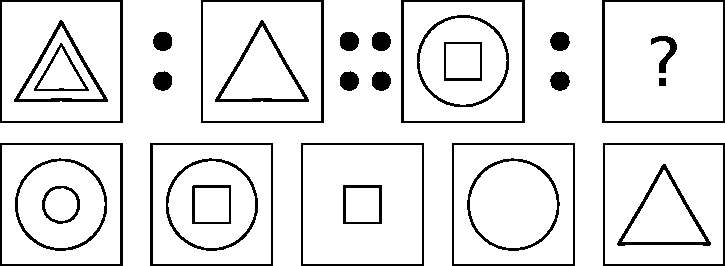
\includegraphics[width=3in]{figures/evans.pdf}
\caption{A geometrical analogy problem: figure $A$ is to figure $B$ as figure
  $C$ is to which candidate?}
\label{FIG:evans}
\end{figure}

The inputs to the program are rough, hand-built low-level descriptions of the
figures. For example, simple geometric shape such as circles, rectangles or
triangles are all described with one single primitive:
\textit{SIMPLE\_CLOSED\_CURVE(\dots)}, where the arguments are the start and
end of the (multiple) lines, and their curvatures. The program is then
divided into two distinct parts.

The role of the first part is to build high level representations of the
figures from these raw descriptions. After identifying coherent shapes (such as
triangle, square, etc.) as independent objects, the program tries to find
relations of the kind \textit{INSIDE(Obj1, Obj2)} or \textit{ABOVE(Obj1, Obj3)}
between figures. Finally, similarities between every pair of objects are
computed. The similarity measure is based on the transformability of the first
object into the second one, using traditional geometrical transformations
(rotation, scale, reflections, etc.). All the information computed by the first
part are given as input (on punched cards!) to the second part.

The second part relates to the analogical solving process per se. Using the
output of the first part, ANALOGY will try to find a set of rules that
transform figure $A$ into figure $B$. A rule would for example state
\textit{REMOVE(Obj1), ROTATE(Obj2, 45\degree)}, etc. Then, by generalizing
each rule, it tries to establish a correspondence between these rules and those
transforming $C$ into one of the candidate solutions. The chosen solution is
the one that maximizes the resemblance between the two sets of rules.

An interesting fact is that ANALOGY analyses the way to go from $A$ to $B$ and
applies it to go from $C$ to $D$, but it does not make use of \textit{central
permutation}\footnote{The central permutation axiom, described in the next
chapter, states that $A:B::C:D \iff A:C::B:D$.}: it may just as well analyze the way to go from $A$ to $C$ and
transpose it to go from $B$ to $D$. Note also that in ANALOGY the semantics
behind the relations and the geometrical objects are not taken into account. In
this respect, ANALOGY is close to Gentner's Structure Mapping Theory (but
preexisting by far).


\subsection{Analogical reasoning as distance minimization on a vector space}
\label{SEC:rumelhart_Abrahamsen}

At a time where most models of analogy used to take the form of complex computer
programs (such as that of Evans), the two cognitive scientists David Rumelhart
and Adele Abrahamsen proposed a simple theoretical model of analogical
reasoning \cite{RumAbr73}. Their model is of great interest for us because as
it will become clear, their view of analogy is in total accordance with our use
of analogy in machine learning (or should we say more humbly that our use of
analogy is fully compliant with their earlier model).

For Rumelhart and Abrahamsen, a human reasoning process can be defined by two
components: a memory structure in which the remembered objects are stored, and
an algorithm that manipulates these data to produce a result. In their paper,
they define these two components for the analogical reasoning.

With regards to the memory structure, their assumption is that it can be
considered as an $m$-dimensional Euclidean space. This assumption is originally
that of Henley \cite{Hen69} who showed, with the help of social experiments,
that a set of 30 mammals could be fairly well represented in the 3-dimensional
space $\mathbb{R}^3$ with the three axes \textit{ferocity}, \textit{humanness},
and \textit{size}. It is supposed that the semantic similarity that people
associate with two concepts is inversely proportional to their distance in the
Euclidean space $\mathbb{R}^3$. For example, \textit{cow} and \textit{horse}
should be fairly close, but \textit{rat} would likely be far from both.

Rumelhart and Abrahamsen are interested in the problem of solving an analogical
equation (although they never state it in these terms): given three concepts
$A, B, C$ and a set of candidate solutions $D_1, D_2, \cdots, D_n$, which $D_i$
is the best candidate for $A:B::C:D_i$? Their assumption is the following:
\textbf{ for a human agent, the best solution is the closest $D_i$ to the
(potentially hypothetical) \textit{perfect} solution $I$, defined as $I = C - A
+ B$}. This principle is illustrated in figure \ref{FIG:rumelhart_model}.
To assess the soundness of this hypothesis, diverse social experiments are led
by the authors. For example, students are asked to choose the best candidates
for various randomly generated analogies, e.g. rat is to pig as goat is to $[$
chimpanzee, cow, rabbit, sheep$]$.

\begin{figure}[!h]
\centering
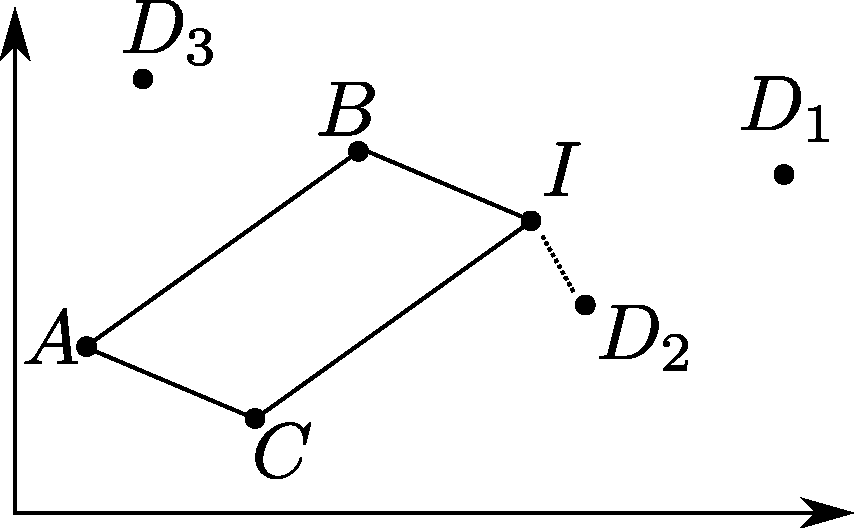
\includegraphics[width=2.5in]{figures/rumelhart_model.pdf}
  \caption{Analogical equation solving process as in \cite{RumAbr73}. The
  solution is here $D_2$.}
\label{FIG:rumelhart_model}
\end{figure}

As it will become clear, this idea that an analogy $A:B::C:D$ is better when
$D$ is \textbf{close} (as measured by a distance on a metric space) to the true
solution $I$ is entirely compatible with the notion of \textit{analogical
dissimilarity} that will be defined in Chapter \ref{CHAP:functional_definition}.

More recently, various techniques have been proposed to generate a vector-space
embedding for words from a large corpus of text documents, for example
Word2Vect \cite{MikCheCorDea13}. In these continuous spaces also, some
interesting analogies between words can be found that give even more power to
the works of Rumelhart and Abrahamsen. The most classical example of
word-analogy in such a space is given by \textit{man} is to \textit{woman} as
\textit{king} is to \textit{queen}, where the vector
\textit{queen} was found to be the one that is the closest to the vector
\textit{king - man + woman}, which is in perfect accordance to the idea of
Rumelhart and Abrahamsen. Other meaningful analogies can be found, and some of
them are illustrated in Figure \ref{FIG:word_analogies}. See \cite{MikYihZwe13}
for more details on finding linguistic regularities in word space embeddings.
\begin{figure}[!h]
\centering
  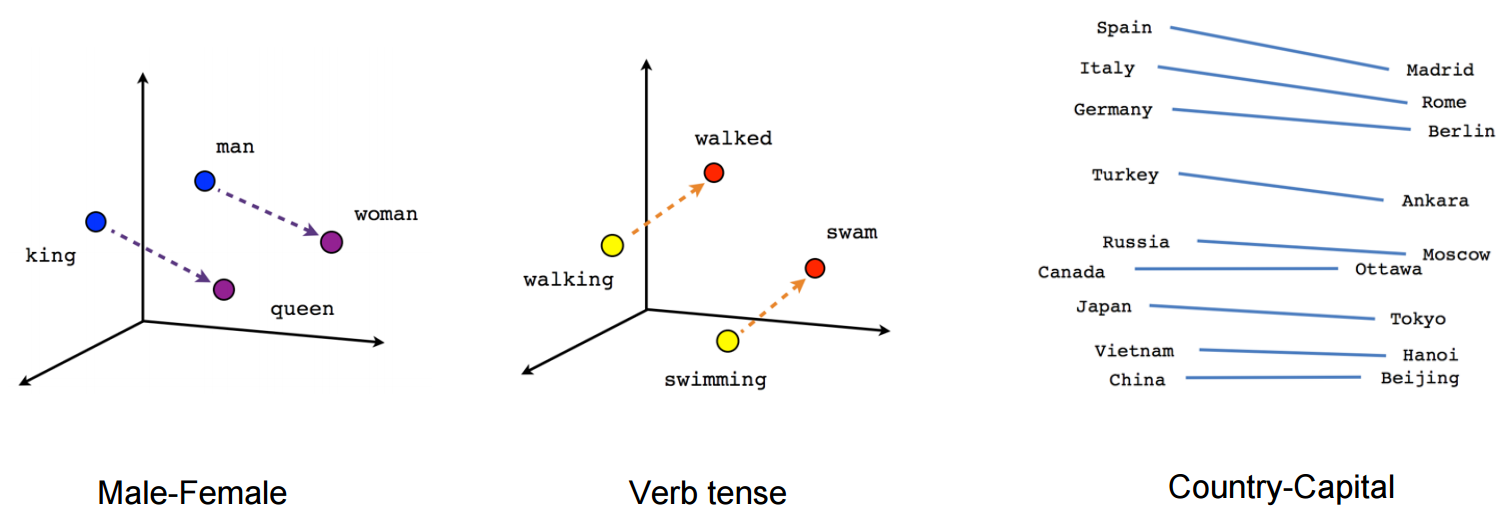
\includegraphics[width=5in]{figures/word_analogies.png}
\caption{Analogies between words in the Word2Vect model. Image source:
  \url{https://www.tensorflow.org/versions/master/tutorials/word2vec}.}
  \label{FIG:word_analogies}
\end{figure}


\subsection{The Copycat program}
\label{SEC:copycat}

Copycat \cite{Mit93} (see also \cite{HofMit94}) is another famous program that
performs analogical reasoning tasks, introduced by Melanie Mitchell and Douglas
Hofstadter. The problems considered by Copycat are the solving of analogical
equations in a \textit{microworld} of strings of letters. A typical Copycat
problem looks as follows:
$$\mathbf{abc} : \mathbf{abd} :: \mathbf{ijk} : x.$$

What should the value of $x$ be? Various answers may be relevant here, such as
$\mathbf{ijd}$ (replace the right-most letter by $\mathbf{d}$), but the most
natural answer probably is $\mathbf{ijl}$: replace the right-most letter by its
successor. How about $\mathbf{zrq}$? Well, not really convincing. The point of
the authors, however, is that \textit{a priori} every single option should be
given equal chances of success.

This principle is strongly reflected in the Copycat program which is
probabilistic in nature: for the same problem, various solutions can be found
depending on the initial condition. For example the  equation $\mathbf{abc} :
\mathbf{abd} :: \mathbf{mrrjjj} : x$ leads to $\mathbf{mrrkkk}$ in 70\% of the
cases (over 1000 experiments), and to $\mathbf{mrjjk}$ 20\% of the time. Other
less plausible solutions make up the remaining 10\%.

At the beginning of the program, each option is equally available.  Then, on
the basis of their validity, some hypotheses are given a stronger chance to
\textit{survive} till the end of the program, while others are discarded.
Conceptually, this process emerges from the interoperability of three main
components: the workspace, the codelets, and the temperature.

\begin{itemize}
    \item The workspace, is the place where objects and relations live.
      In the workspace, diverse conceptual structures are built-in:
      \textit{successor}, \textit{predecessor}, \textit{left-most},
      \textit{right-most}, \textit{orientation}, etc. When the program starts, none of these
      structures are activated: this will be the role of the codelets.
    \item The codelets, are competing agents trying to explore and build
      perceptual structures and relations between the objects in the workspace.
      Their behaviour depends on the temperature.
    \item The temperature could be also defined as the entropy of the
      system. When relations in the workspace are strong and well established,
      the temperature is low. At the beginning of the program, the temperature
      is the highest, leading to a multitude of codelets being run in every
      single \textit{direction}. This concept of temperature can be viewed as
      the trade-off between exploration (trying every possible hypothesis) and
      exploitation (the actual use of a well established hypothesis). When the
      temperature goes below a given threshold, the program stops and the
      current hypothesis is outputted.
\end{itemize}

\begin{figure}[!h]
\centering
  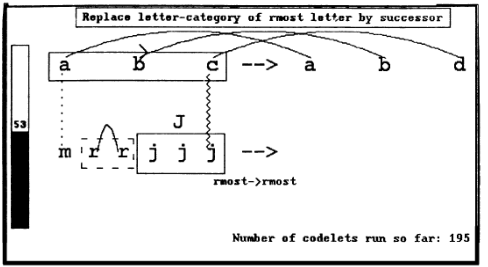
\includegraphics[width=3.5in]{figures/copycat.png}
\caption{Snapshot of Copycat during an equation solving process. Image taken
  from \cite{Mit01}.}
\label{FIG:copycat_snapshot}
\end{figure}

Figure \ref{FIG:copycat_snapshot} illustrates the internal state of Copycat
during the solving of $\mathbf{abc} : \mathbf{abd} :: \mathbf{mrrjjj}: x$. 195
codelets have run so far, so the temperature is average and some structure have
been properly established, such as the \textit{successor group} $\mathbf{abc}$
and the \textit{sameness group} $\mathbf{jjj}$. The $\mathbf{rr}$ group is also
being defined, though still weaker than the others at this stage. Also, a rule
describing the change from $\mathbf{abc}$ to $\mathbf{abd}$ has been
established: \textit{replace the right-most letter by its successor}. Depending
on the future behaviour of the codelets, this rule with either stick till the
end of the program or change to lead to the most common prediction $x =
\mathbf{mrrkkk}$.

Copycat is clearly a complex adaptative system where a global behaviour emerges
from small, independent parts. According to its authors, \textit{Copycat's
architecture is neither symbolic nor connectionist, nor a hybrid of the two;
rather, the program has a novel type of architecture situated somewhere in
between these extremes}.

\subsection{Analogy and the Minimum Description Length Principle}
\label{SEC:analogy_and_the_minimum_decsription_length_principle}

Ockham's razor (also Occam), due to the Franciscan philosopher William
of Ockham (1285~-~1347), is a well known principle in machine learning theory.
The main and most useful interpretation of the original Latin version states
that when trying to explain a situation, if two hypotheses give the same answer
then the best one is probably the \textbf{simplest} one. In practice, what
makes an hypothesis simple remains quite vague, at least from a computational
point of view. Yet this principle has been formalized into Rissanen's Minimum
Description Length Principle (MDLP) \cite{Ris78}, which is based on Kolmogorov
complexity. Despite the difficulty to build inferential models from this
principle (Kolmogorov complexity is often intractable and impossible to
compute, and can only be estimated), it has shown to be quite influential in
the field of machine learning, at least from a theoretical point of view.

With this in mind, Antoine Cornuéjols proposed a framework for assessing the
quality of an analogy \cite{CorMLS96} (see also \cite{CorJFA96}). In these
papers, Cornuéjols hypothesizes that the best analogy between a source and a
target model is the \textit{simplest} one, meaning that its description length
is minimal, in terms of Kolmogorov complexity.

Let us first recall some basic knowledge about Kolmogorov complexity,
before diving into more technical details. The Kolmogorov complexity of a
string of characters $x$, denoted $K(x)$, is the length of the shortest
computer program capable of outputting $x$ on a universal Turing machine. $K(x)$ is supposed to capture the
intrinsic complexity of $x$. Intuitively, $K('aaaaabbbbb')$ is supposed to be
lower than $K('abaabbabab')$, because a clear pattern emerges in the first
string, leading to a simple program: first print $a$ five times, then do the
same for $b$. The second string seems more or less random, which makes it
difficult to factorize into a concise program. In some sense, the Kolmogorov
complexity captures how well a string $x$ can be \textit{compressed}. The
conditional complexity $K(x \given y)$ is the size of the shortest program that
outputs $x$ when given $y$ as an input.

Now, let's get back to our analogical concerns. As illustrated in figure
\ref{FIG:cornuejols_model}, Cornuéjols considers an analogy as a process
involving an object $x_S$ in a source domain, an object $x_T$ in a target
domain, and two functions $f_S$ and $f_T$ transforming $x_S$ and $x_T$ into
$y_S$ and $y_T$ respectively: $y_S = f_S(x_S)$ and $y_T = f_T(x_T)$. Each
domain $S$ and $T$ \textit{lives} inside a theory or model (namely $M_S$ and
$M_T$), that can describe their corresponding objects.

\begin{figure}[!h]
\centering
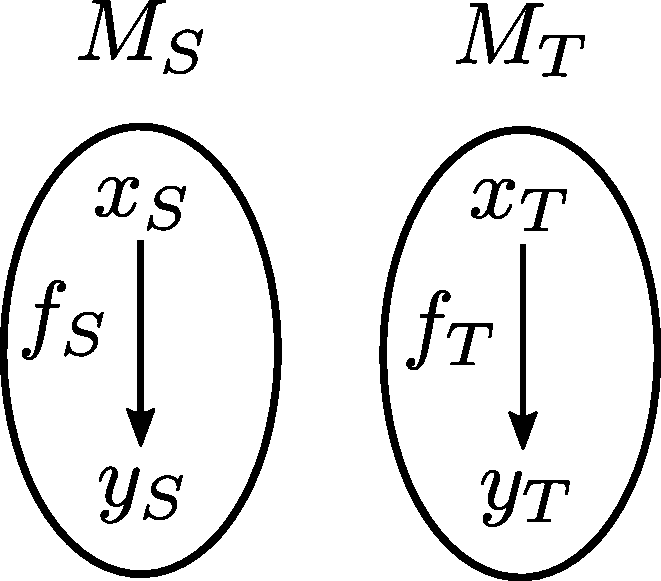
\includegraphics[width=1.5in]{figures/cornuejols_model.pdf}
\caption{The two domains $S$ and $T$ in Cornuéjols' model.}
\label{FIG:cornuejols_model}
\end{figure}

For Cornuéjols, the best analogy is the one that minimizes the following sum of
Kolmogorov complexities:
$$K(M_S) + K(x_S \given M_S) + K(f_S \given M_S) + K(M_T \given M_S) + K(x_T
\given M_T) + K(f_T \given M_T),$$
where:
\begin{itemize}
   \item $K(M_S)$ is the cost associated with the source theory,
   \item $K(x_S \given M_S)$ is the cost of $x_S$ as described in the source
     theory,
   \item $K(f_S \given M_S)$ is the cost of $f_S$ as described in the source
     theory,
   \item $K(M_T \given M_S)$ is the cost of describing the target theory from
     the source theory,
   \item $K(x_T \given M_T)$ is the cost of $x_T$ as described in the target
     theory,
   \item and finally $K(f_T \given M_T)$ is the cost of $f_T$ as described in
     the target theory.
\end{itemize}

Notice that the terms $y_i$ are not considered in this cost function, because
they are entirely defined by their corresponding $x_i$ and $f_i$.

Cornuéjols illustrates the plausibility of his model using experiments in the
microworld of Copycat. After defining the Kolmogorov complexity of the built-in
relations (\textit{direction}, \textit{length}, etc.), and those of the
representations of the inputs, the solutions of the analogical equations are
set as those minimizing the above criterion. The empirical results show that
this model, in addition to its theoretical appeal due to the proximity with
MDLP, is at the very least an interesting option that deserves further
investigations. In a recent work, this model of analogy has been applied to a
task of transfer learning \cite{CorMur16}.

Adopting a different (but close) approach, the association between Kolmogorov
complexity and the evaluation of the quality of an analogy has also been
recently advocated in \cite{BayPraRic12}. In this work, the authors propose
that if four objects $a, b, c, d$ are in proportion, then it should be as
\textit{complicated} to go from $a$ to $b$ as to go from $c$ to $d$, and it
should also be as \textit{complicated} to go from $b$ to $a$ as to go from $d$
to $c$. More formally:
$$a:b::c:d \implies K(b \given a) = K(d \given c) \text{ and } K(a \given b) =
K(c \given d).$$
This criterion was used to automatically discriminate \textit{good} analogies
from \textit{bad} analogies, where objects were concepts represented as words
of the natural language, and where their Kolmogorov complexity was roughly
approximated using online search-engine queries. The experiments showed that
the system was able to differentiate credible analogies from fishy ones in
about 75\% of the time.

\subsection{Case-Based Reasoning}

We will here describe the field of Case-Based Reasoning (CBR). First of all,
let us note that CBR is not literally a computational model of analogy, but is
rather a general problem solving paradigm that makes use of some particular
form of analogical reasoning. As discussed in \cite{AamPla94}, CBR and
analogical reasoning are often mixed up in the literature.  We choose to
briefly describe CBR now, because we need to clarify how our approach to
problem solving will differ from that of CBR.

CBR is a very general paradigm for problem solving, where a new problem is
solved using the knowledge of some similar past experiences. This model can be
motivated by its psychological appeal: it is indeed well acknowledged that,
when confronted with an unknown situation, humans tend to make use of their
past knowledge about some other similar situation to solve the problem at hand.
As an example, the recipe of a strawberry pie could be easily inferred using
the past knowledge on the recipe of other fruit pies (e.g. apple pie, pear pie,
etc.).

In its most general form, CBR is a way of reaching the unknown solution $S$ to a
problem $P$ using the known solutions $S_i$ to problems $P_i$ that are
\textbf{similar} to $P$. Each pair $(S_i, P_i)$ is called a \textbf{case},
hence the name of the paradigm.  The term \textit{problem} is here used in its
most general sense.  In \cite{AamPla94}, a CBR process is described by the
succession of the following four steps:
\begin{enumerate}
  \item \textbf{Retrieve}: this first step is to retrieve all cases $(S_i,
    P_i)$ where $P_i$ is similar to the initial problem $P$. The way these
    cases are chosen is entirely dependent of the current setting, and greatly
    differ depending on the application. Sometimes, only a single case  is
    selected.
  \item \textbf{Reuse}: the solutions $S_i$ associated to the most relevant
    $P_i$ are aggregated in some way, and adapted if needed to build up the
    final solution $S$.
  \item \textbf{Revise}: the relevance and the adequacy of the chosen solution
    $S$ are evaluated, and $S$ is modified if needed.
  \item \textbf{Retain}: if the revised solution $S$ ended up being a good
    choice, then the solution is retained and the pair $(P, S)$ is bound to
    be used in the solving of some future problems.
\end{enumerate}

%%Quite amusingly, the CBR community tends to see analogical reasoning as a
%%subfield of CBR, while the analogical reasoning community seems to believe that
%%CBR is a particular instance of analogy-based reasoning. Indeed in
%%\cite{AamPla94}, the authors (that are CBR oriented) define analogical
%%reasoning as a particular CBR instance that is focused on solving cross-domain
%%problems, i.e. where a problem in a source domain has to be mapped into a
%%problem in a target domain. While this description of analogical reasoning is
%%fairly reasonable, one may object that what defines the source and target
%%domains is completely arbitrary, thus reducing CBR to a particular instance of
%%analogical reasoning where the source and target domains are forced to be the
%%same.
%%
%%We will not further discuss this point here but

Before moving further to the next chapter, we would like to point out a
significant difference between the CBR approach and the one we will address in
this document. In a way, the CBR process can be viewed as building the
following analogical proportions:
$$P_i:S_i :: P : S, $$
where $S$ is unknown and inferred from all the $S_i$. We can indeed consider
that \textit{problem $P_i$ is to solution $S_i$ as problem $P$ is to solution
$S$}. Each of these analogical proportions is built on the basis that $P_i$ and
$P$ are \textbf{similar}, so $S$ should be similar to $S_i$.

But as we will see in the next chapter, an analogical proportion $a:b::c:d$ is
not restricted to having $a$ close to $c$ and $b$ close to $d$! It is quite the
contrary actually: all elements are allowed to be extremely distinct. And
indeed, if we are able to \textit{capture} how a given $P_i$ (that is not close
to $P$) differs from $P$, then applying the same transformation to $S_i$ should
give us a relevant potential solution $S$.  Acknowledging this fact, our
approach to analogical learning will rather follow another conceptual
scheme: we will try to retrieve the proportions of the form $P_{i_1} : P_{i_2}
:: P_{i_3} : P$, and the solution $S$ will be inferred by
\textit{extrapolation}\footnote{The way $S$ is \textit{extrapolated} will be
described in the next chapter as the \textbf{solving} of the analogical
equation.} from the associated equations: $S_{i_1} : S_{i_2} :: S_{i_3} :
S$. This allows us to consider problems $P_i$ that are both similar
\textbf{and} different from $P$, which may allow to find more interesting
solutions $S$.

\section*{Conclusion}

This first chapter was devoted to the description of past works on the modeling
of analogical reasoning. We chose here to distinguish between two groups of
models: those that make explicit use of analogical proportions (either as a key
component of the model or as a simple use-case example), and those that do not.
Among the models that use analogical proportions, we will see that the model
of Rumelhart and Abrahamsen (derived from a psychological perspective) will be
in perfect accordance to our view of analogical classification, and analogical
learning in general.

It is fairly clear that these past works are, with a few exceptions, mostly
motivated by cognitive and psychological investigations. It is only recently
that some authors \cite{FedPirYvo95, LepShi96} have provided a formal framework
to deal with analogical proportions in general algebraic settings, which opened
the door to many computational applications. These formal analogical
proportions are a key concept for our work. We will now review this topic in
the next chapter.

\paragraph{Résumé du chapitre}

D'une façon générale, une analogie établit des parallèles entre deux situations
différentes. Le raisonnement par analogie permet alors d'inférer des propriétés
sur l'une des situations, en utilisant nos connaissances de l'autre situation.
Un type particulier de raisonnement par analogie est celui lié aux proportions
analogiques, qui sont des expressions de la forme \textit{a est à b ce que c
est à d}, souvent écrit $a:b::c:d$. Là aussi, on peut parfois déduire la valeur
d'un des quatre éléments sur la base de notre connaissance des trois premiers.
Ce processus s'appelle la \textit{résolution d'équation analogique}.

Les deux premiers chapitres de ce document seront dédiés à fournir les
prérequis nécessaires concernant les modèles de raisonnement par analogie, et
en particulier ceux relatifs aux proportions analogiques. Dans ce premier
chapitre nous décrivons brièvement différentes tentatives de formaliser le
raisonnement par analogie, accordant une attention particulière aux modèles qui
peuvent s'utiliser à des fins inférentielles.

Nous avons choisi ici de faire la distinction entre deux types de modèles :
ceux qui ne font jamais référence aux proportions analogiques, et ceux qui
recourent aux proportions analogiques d'une manière ou d'une autre: les
proportions sont alors soit une composante clef du modèle (par exemple sections
\ref{SEC:solving_geometric_proportions} et \ref{SEC:rumelhart_Abrahamsen}),
soit une simple possibilité d'application (sections \ref{SEC:copycat} et
\ref{SEC:analogy_and_the_minimum_decsription_length_principle}).

Ces différentes propositions sont, en grande partie, inspirées par des travaux
provenant des sciences cognitives et psychologiques. Ce n'est qu'assez
récemment que certains auteurs, partant des premiers travaux de Lepage
\cite{Lep04}, ont proposé divers modèles formels permettant l'usage des
proportions analogiques au sein de structures algébriques. Ces
proportions analogiques sont le principal objet de nos travaux, et nous les
décrivons en détail dans le prochain chapitre.



\chapter{Formal analogical proportions}
\label{CHAP:formal_analogical_proportions}
\localtableofcontents*
\vspace*{\baselineskip}

\initial{A}fter a first introduction of past works on analogical reasoning in
Chapter \ref{CHAP:computational_models_of_analogical_reasoning}, we will now
provide all the necessary background on formal analogical proportions, the most
important concept of this document.

An \textbf{analogical proportion} is a statement of the form ``$a$ is to $b$ as
$c$ is to $d$''. It is a relation between the two pairs $(a,b)$ and $(c,d)$,
which expresses that what is common to $a$ and $b$ is also common to $c$ and
$d$, and what is different between $a$ and $b$ is also different between $c$
and $d$. There are numerous examples of such statements, with which everybody
will more or less agree, such as  ``a calf is to a cow as a foal is to a
mare'', or ``Paris is to France as Berlin is to Germany''.  As a relation
involving both similarities \textbf{and} dissimilarities between four objects,
an analogical proportion is able to model complex associations.

\paragraph{The three axioms of analogical proportions\\}

It has been agreed since Aristotle time that an analogical proportion $A$ is a
quaternary relation satisfying the \textbf{three following axioms}, for any $a,
b, c, d$:

\begin{enumerate}
\item $A(a,b,a,b)$ always holds (Reflexivity)
\item $A(a,b,c,d) \implies A(c,d,a,b)$ (Symmetry)
\item $A(a,b,c,d) \implies A(a,c,b,d)$ (Central permutation)
\end{enumerate}

When there is no ambiguity over $A$ and its domain, the infix notation
$a:b::c:d$ is often used. Considering again the farm example, the symmetry
axiom states that if a calf $(a)$ is to a cow $(b)$ as a foal $(c)$ is to a
mare $(d)$, then a foal $(c)$ is to a mare $(d)$ as a calf $(a)$ is to a cow
$(b)$, which seems perfectly sound. The central permutation axiom leads to the
natural consequence that a calf $(a)$ is to a foal $(c)$ as a cow $(b)$ is to a
mare $(d)$.

This chapter is structured as follows. In the first section of this chapter, we
will provide the definition of analogical proportions in various settings, with
a strong emphasis on the arithmetic and Boolean proportions, which will turn
out to be very close. We will further investigate this bond in the second
section, which will be devoted to describe these two proportions from a
geometrical perspective. In the last section, we will consider a toy
classification problem, which will help us introduce two other key concepts:
the \textbf{analogical inference principle}, and the process of
\textbf{analogical equation solving}. This last section will also serve as a
transition towards the next chapter, which will be devoted to describe our
contributions to analogical classification.

\section{Formal definitions}
\label{SEC:formal_definitions_proportions}

The goal of this first section is to provide the definitions of analogical
proportions in various settings. We will particularly focus on the arithmetic
proportion that deals with real numbers, and on the Boolean proportion.

\subsection{The geometric and arithmetic proportions}

\paragraph{A factorization-based definition of analogical proportions\\}

Probably the first use of formal proportions is that of Lepage in \cite{Lep04}
who, starting from the three aforementioned axioms, formally defined analogical
proportions over alphabets of letters with the aim of generating (analogical)
formal languages. His definition have later been generalized in the works of
Stroppa and Yvon (see \cite{StrYvoCNLL05} and \cite{StrYvoREPORT05}), who
provided an algebraic factorization-based definition of analogical proportions
in semigroups:

\begin{definition}[Proportion in semigroups]
\label{DEF:proportion_semi_group}
Let $(U, \oplus)$ be a semigroup, i.e. $U$ is a set and $\oplus$ is an
  associative binary operation. Four elements $a, b, c, d \in U$, are in proportion if
  there exists some factorization
  \begin{align*}
    a &= a_1 \oplus a_2 \oplus \cdots \oplus a_n\\
    b &= b_1 \oplus b_2 \oplus \cdots \oplus b_n\\
    c &= c_1 \oplus c_2 \oplus \cdots \oplus c_n\\
    d &= d_1 \oplus d_2 \oplus \cdots \oplus d_n,
  \end{align*}

  such that for all $i \in [1, n]$,
  $$
  \begin{cases}
    a_i = b_i \text{ and } c_i = d_i\\
    \text{or}\\
    a_i = c_i \text{ and } b_i = d_i.
  \end{cases}
  $$
\end{definition}

\begin{testexample}
  A use of this definition can be found in \cite{StrYvoREPORT05}, where
  the authors define an analogy between words of a finite alphabet using the
  concatenation operator, which allows to build proportions such as:
  $$\text{eat} : \text{eating} :: \text{look} : \text{looking}.$$ This analogy
  was used in an automatic verb conjugation task that we will briefly describe
  in the next chapter.
\end{testexample}

\paragraph{Analogical proportions between real numbers\\}

To further illustrate the use of Definition \ref{DEF:proportion_semi_group}, it
will be insightful to instantiate $U$ as the set of natural number $\mathbb{N}$
and $\oplus$ as the usual multiplication $\times$.
\begin{testexample}
  In this setting, let's consider the prime factorization of:

  \begin{align*}
    a &= 30 = 1 \times 2 \times 3 \times 5\\
    b &= 60 = 2 \times 2 \times 3 \times 5\\
    c &= 25 = 1 \times 1 \times 5 \times 5\\
    d &= 50 = 2 \times 1 \times 5 \times 5
  \end{align*}

For each $i$, we either have $a_i = b_i$ and $c_i = d_i$ ($i = 2, 3, 4$) or
$a_i = c_i$ and $b_i = d_i$ ($i = 1, 4$). We can then say that $a, b, c, d$ are
in proportion, i.e. $30: 60 :: 25: 50$. We recognize here the \textbf{geometric
  proportion}: $\frac{30}{60} = \frac{25}{50}$.
\end{testexample}

\begin{definition}[Geometric proportion]
  Four elements $a, b, c, d$ in $\mathbb{R}$ are in \textbf{geometric
  proportion} if
  $$\frac{a}{b} = \frac{c}{d},$$
  or equivalently if
  $$a\times d = b\times c.$$
\end{definition}

It now becomes clear why analogical proportions are effectively called
\textit{proportions}: it is precisely because they generalize the well-known
numerical geometric proportion to more complex structures.  Actually, Aristotle
stated the three aforementioned axioms on the basis of the geometric
proportion.

In fact, when $\mathbb{R}$ is equipped with the multiplication $\times$, the
couple $(\mathbb{R}, \times)$ is a group (i.e. a set equipped with an operation
that satisfies  closure, associativity, identity and invertibility). When
dealing with a group (instead of a semigroup), Definition
\ref{DEF:proportion_semi_group} can be greatly simplified:

\begin{definition}[Proportion in groups]
  \label{DEF:proportion_group}
Let $(U, \oplus)$ be a group.  Four elements $a, b, c, d \in U$, are in
  proportion if:
  $$a \oplus d = b \oplus c.$$
\end{definition}

The geometric proportion is clearly a direct instance of this definition.
Another proportion can be defined over real numbers, using this time the
addition operator $+$ for the group $(\mathbb{R}, +)$:

\begin{definition}[Arithmetic proportion]
  Four elements $a, b, c, d$ in $\mathbb{R}$ are in \textbf{arithmetic
  proportion} if:
  $$a + d = b + c,$$
  or equivalently if
  $$a - b = c - d.$$
\end{definition}

\paragraph{Analogical proportions over vectors\\}

An analogical proportion in $\mathbb{R}$ is great, but what will be more useful
is a proportion in $\mathbb{R}^m$, so that we can deal with vectors.  Let us
make a brief notation note: in the rest of this document, vectors will be
denoted by boldface letters and their components will be denoted by regular
letters. For example, a vector $\mathbf{x} \in X^m$ will be defined as
$\mathbf{x} = (x_1, x_2, \dots, x_m)$.

It is actually fairly easy to define a proportion in a given set $X^m$ provided
that we already have a proportion in $X$. Indeed, a natural extension to $X^m$
is to require that each of the $m$ dimensions make up valid proportions in $X$:

\begin{definition}[Proportion for vectors]
  \label{DEF:analogy_for_vectors}
  Let $A$ be an analogy over a set $X$. We can define an analogy $A^m$ over
  $X^m$ in a component-wise fashion by:
  $$A^m(\mathbf{a}, \mathbf{b}, \mathbf{c}, \mathbf{d}) ~ \text{  if  } ~
  A(a_i, b_i, c_i, d_i) \text{ for all } i \in [1, m],$$
  where $\mathbf{a}, \mathbf{b}, \mathbf{c}, \mathbf{d}$ are vectors in $X^m$.
  More often than not, $A^m$ will simply be denoted $A$ for the sake of
  brevity.
\end{definition}
\noindent
Thanks to Definition \ref{DEF:analogy_for_vectors}, we now have the definition
of two numerical proportions in $\mathbb{R}^m$: one that generalizes the
geometric proportion and one that generalizes the arithmetic proportion.  The
interpretation of the geometric proportion in $\mathbb{R}^m$ can be opaque, but
that of the arithmetic proportion is very clear: four vectors $\mathbf{a},
\mathbf{b}, \mathbf{c}, \mathbf{d}$ of $\mathbb{R}^m$ are in arithmetic
proportion if $\mathbf{a} - \mathbf{b} = \mathbf{c} - \mathbf{d}$, i.e.
\textbf{if they are the four vertices of a parallelogram}, as illustrated in
Figure \ref{FIG:arithmetic_proportion}.
\begin{figure}[!h]
\centering
  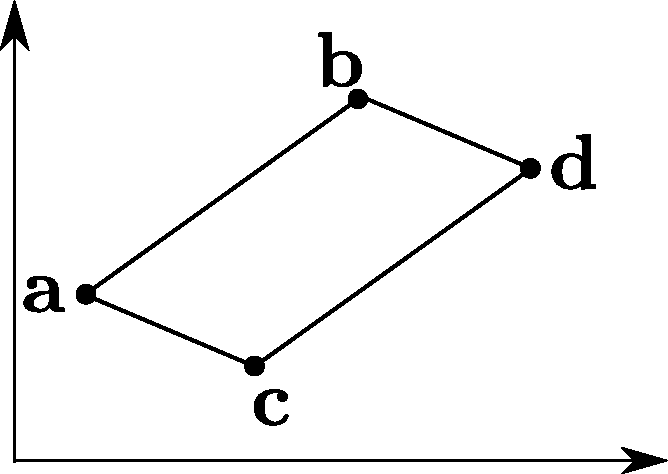
\includegraphics[width=2.5in]{figures/arithmetic_proportion.pdf}
  \caption{$\mathbf{a}, \mathbf{b}, \mathbf{c}, \mathbf{d}$
  are in arithmetic proportion iff they are the four vertices of a
  parallelogram.}
\label{FIG:arithmetic_proportion}
\end{figure}

Let us mention that even if they did not explicitly mention the parallelogram
view of analogy, Rumelhart and Abrahamsen (Section
\ref{SEC:rumelhart_Abrahamsen}) clearly used the arithmetic proportion for
their psychological model of analogical reasoning.

Starting from the general lines of Definition \ref{DEF:proportion_semi_group},
other proportions have been defined in various domains, e.g. analogies
between trees, lattices, or matrices \cite{MicDel04, StrYvoREPORT05,
MicBayDelJAIR08}. However, we will not detail them further here and rather
focus on other domains of interest, namely analogies between sets. Defining
analogies between sets will indeed allow us to derive the definition of an
analogical proportion for Boolean values, which is the main subject of this
document.

\subsection{Analogical proportions between sets}

In \cite{Lep03}, Lepage defines an analogy between sets as follows: four subsets
$A, B, C, D$ of a universal set $X$ are in proportion if $A$ can be transformed
into $B$ by adding and deleting the same elements as to transform $C$ into $D$.
A more formal definition has been given in \cite{StrYvoREPORT05}:

\begin{definition}[Proportion between sets (i)]
  \label{DEF:analogy_set_facto}
  Let $A, B, C, D \subset X$. $A, B, C, D$ are in proportion if there exists
  four subsets $U, V, W$ and $Z$ (not necessarily disjoint) such that:
  $$
  \begin{cases}
    A = U \cup V\\
    B = U \cup W\\
    C = Z \cup V\\
    D = Z \cup W\\
  \end{cases}
  $$
\end{definition}

The requirements of Lepage are clearly respected here: to go from $A$ to $B$,
one needs to add $W$ and remove $V$. To go from $C$ to $D$, one needs to do the
exact same thing: add $W$ and remove $V$. This definition is completely
compliant with our informal introduction at the beginning of this chapter,
where we explained that an analogical proportion $a:b::c:d$ expresses that
\textit{what is common to $a$ and $b$ is also common to $c$ and $d$, and what
is different between $a$ and $b$ is also different between $c$ and $d$}.


An equivalent definition of analogy between sets has been given in
\cite{MicPra09}:

\begin{definition}[Proportion between sets (ii)]
  \label{DEF:analogy_set_miclet_henri}
  Let $A, B, C, D \subset X$. $A, B, C, D$ are in proportion if:
  $$
  A \setminus B = C \setminus D \text{ and } B \setminus A = D \setminus C
  $$
\end{definition}

Definition \ref{DEF:analogy_set_miclet_henri} reads as \textit{$A$ differs from
$B$ as $C$ differs from $D$, and $B$ differs from $A$ as $D$ differs from $C$},
which is naturally equivalent to the statement of Definition
\ref{DEF:analogy_set_facto}: $A \setminus B = C \setminus D = V$, and $B
\setminus A = D \setminus A  = W$.  Finally, a last equivalent definition can
be given as follows (not without using various ingenious tweaks):

\begin{definition}[Proportion between sets (iii)]
  \label{DEF:yet_other_equiv_def}
  Let $A, B, C, D \subset X$. $A, B, C, D$ are in proportion if:
  $$ A \cap D = B \cap C \text{ and } A \cup D = B \cup C.$$
\end{definition}

\noindent
These three equivalent definitions are illustrated in Figure
\ref{FIG:equiv_analogies_sets}.

\begin{figure}[!h]
\centering
  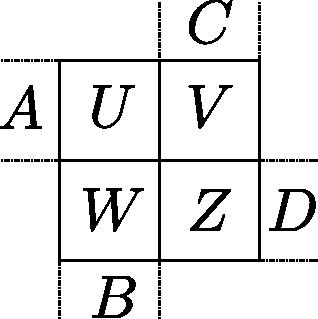
\includegraphics[width=1in]{figures/subset_analogies.pdf}
  \caption{The four sets $A, B, C, D$ are in proportion. In general, $U, V,W,
  Z$ do not need to be disjoint.}
\label{FIG:equiv_analogies_sets}
\end{figure}

\begin{testexample}
For a more concrete example, let us consider $A = \{a, b, c, g\}, B = \{a, b,
d, e, g\}, C = \{c, f, g\}$ and $D = \{d, e, f, g\}$, as summed-up in Table
\ref{TAB:analogy_sets}.
Setting $U = \{a, b, g\}, V = \{c\}, W = \{d, e\}$ and $Z = \{f, g\}$, the
conditions of Definition  \ref{DEF:analogy_set_facto}  are clearly satisfied.
Also, $A \setminus B = C \setminus D = \{c\} = V$, and $B\setminus A = D
\setminus C = \{d, e\} = W$. Finally, $A \cup D = B \cup C = \{a, b, c, d, e,
f, g\}$ and $A\cap D = B\cap C = \{g\}$.
\end{testexample}
\begin{table}[h!]
\centering
$$
\begin{tabular}{ c  c  c  c  c  c  c  c }
\toprule
  & a & b & c & d & e & f & g\\
\midrule
  A & \times & \times & \times &  &  &  & \times \\
  B & \times & \times &  & \times & \times &  & \times\\
  C &  &  & \times &  &  & \times & \times\\
  D &  &  &  & \times & \times & \times & \times\\
\bottomrule
\end{tabular}
$$
\caption{Four sets $A, B, C, D$ in analogical proportion.}
\label{TAB:analogy_sets}
\end{table}

Analogies between sets are important because they allow us to derive the
definition of the Boolean proportion, which is the object of the next
subsection.

\subsection{The Boolean proportion}

\paragraph{Formal definition\\}

We are now in a position to give a formal definition of the Boolean proportion,
which can be directly derived from Definitions
\ref{DEF:analogy_set_miclet_henri} or \ref{DEF:yet_other_equiv_def} by
considering the set $\mathbb{B} = \{0, 1\}$:

\begin{definition}[Boolean proportion (i)]
  \label{DEF:boolean_proportion}
  Four elements $a, b, c, d$ in $\mathbb{B} = \{0, 1\}$ are in proportion if
  \begin{align*}
    &\left[(a \wedge \neg b) \leftrightarrow (c \wedge \neg d)\right]  \wedge
    \left[(\neg a \wedge b)\leftrightarrow (\neg c \wedge d)\right], \text{ or equivalently}\\
    &  (a \wedge d \leftrightarrow b \wedge c) \wedge (a \vee  d
    \leftrightarrow b \vee c),
  \end{align*}
  where $\leftrightarrow$ stands for the equivalence connective.
\end{definition}

The first expression is the direct counterpart of Definition
\ref{DEF:analogy_set_miclet_henri}, and states that \textbf{$a$ differs from
$b$ as $c$ differs from $d$, and conversely $b$ differs from $a$ as $d$ differs
from $c$}.  The second expression directly comes from Definition
\ref{DEF:yet_other_equiv_def}.

In a Boolean setting, there are exactly $2^4 = 16$ different valuations of $a,
b, c, d$. Definition \ref{DEF:boolean_proportion} tells us that exactly $6$ of
these valuations (or \textbf{patterns}) lead to valid Boolean proportions.
Table \ref{TAB:six_valid_patterns} illustrates the $6$ valid patterns and the
$10$ invalid ones. We recognize in Table \ref{TAB:six_valid_patterns} that all
the valid patterns express that we need to perform the same operation to go
from $a$ to $b$ as to go from $c$ to $d$, and that this is not the case for the
invalid patterns. This is compliant with what we expect from an analogical
proportion, as discussed earlier. With regards to this, the last two invalid
patterns (namely $0:1::1:0$ and its counterpart $1:0:0:1$) have a particular
status: we could indeed claim that they express the fact that $b$ is the
negation of $a$ just like $c$ is the negation of $d$, so in some sense we
\textbf{still} could say that $a$ differs from $b$ as $c$ differs from $d$. We
will discuss this point further when we will mention the works of Sheldon
Klein, who came up with a different definition of the Boolean analogical
proportion.

\begin{table}[t]
  \centering
  \begin{tabular}[t]{ccccc}
    \toprule
    $a$ & $b$ & $c$ & $d$ &  $A(a, b, c, d)$\\
    \midrule
    0 & 0 & 0 & 0 &   \textbf{1}\\
    1 & 1 & 1 & 1 &   \textbf{1}\\
    0 & 0 & 1 & 1 &   \textbf{1}\\
    1 & 1 & 0 & 0 &   \textbf{1}\\
    0 & 1 & 0 & 1 &   \textbf{1}\\
    1 & 0 & 1 & 0 &   \textbf{1}\\
    \bottomrule
  \end{tabular}
  ~~~~
  \begin{tabular}[t]{ccccc}
    \toprule
    $a$ & $b$ & $c$ & $d$ &  $A(a, b, c, d)$\\
    \midrule
    0 & 0 & 0 & 1 &   \textbf{0}\\
    0 & 0 & 1 & 0 &   \textbf{0}\\
    0 & 1 & 0 & 0 &   \textbf{0}\\
    1 & 0 & 0 & 0 &   \textbf{0}\\
    1 & 1 & 1 & 0 &   \textbf{0}\\
    1 & 1 & 0 & 1 &   \textbf{0}\\
    1 & 0 & 1 & 1 &   \textbf{0}\\
    0 & 1 & 1 & 1 &   \textbf{0}\\
    0 & 1 & 1 & 0 &   \textbf{0}\\
    1 & 0 & 0 & 1 &   \textbf{0}\\
    \bottomrule
  \end{tabular}
  \caption{The six valid patterns of the Boolean proportion (left), and the ten
  invalid patterns (right).}
  \label{TAB:six_valid_patterns}
\end{table}

We observe from Table \ref{TAB:six_valid_patterns} that some
sort of {\it code independence axiom} is satisfied, which guarantees that $0$
and $1$ play symmetric roles:
\begin{property}
  \label{PROPER:code_indep}
  Let a, b, c, d in $\mathbb{B}$. Then
  $$a : b :: c : d \iff \neg a :  \neg b ::  \neg c :  \neg d,$$
  where $\neg x$ is the negation of $x$.
\end{property}
This code independence property is actually extremely important for
representational purposes, because it means that we do not have to care about
the coding convention of the Boolean vectors that we use.

We gave the definition of the Boolean proportion as a consequence of the
definition of proportions between sets, but let us note that in fact, the $6$
valid patterns of Table \ref{TAB:six_valid_patterns} could have been derived
directly from the $3$ axioms of an analogical proportion: the first axiom tells
us that the proportion $a:b::a:b$ holds for any value of $a$ and $b$ in
$\mathbb{B}$. This means that the four following proportions are valid:
\begin{itemize}
  \item $0 : 1 :: 0 :1$ ;
  \item $1 : 0 :: 1 :0$ ;
  \item $0 : 0 :: 0 :0$ ;
  \item $1 : 1 :: 1 :1$.
\end{itemize}
Using the central permutation axiom $(a:b::c:d \iff a:c::b:d$), we can then
derive two additional proportions, which makes a total of $6$ proportions that
are indeed those of Table \ref{TAB:six_valid_patterns}:
\begin{itemize}
  \item $1 : 1 :: 0 : 0$ ;
  \item $0 : 0 :: 1 : 1$.
\end{itemize}

\paragraph{The Boolean proportion as a particular case of the arithmetic
proportion\\}

By paying attention to Table \ref{TAB:six_valid_patterns}, we notice that the
Boolean proportion can actually be defined in a simpler way:
\begin{definition}[Boolean proportion (ii)]
  \label{DEF:boolean_proportion_informal}
  Four elements $a, b, c, d$ in $\mathbb{B}$ are in proportion if:
  $$
  \begin{cases}
    a = b \text{ and } c = d\\
    \text{or}\\
    a = c \text{ and } b = d,
  \end{cases}
  $$
  or equivalently if
  $$a - b = c - d.$$
\end{definition}

Naturally, the values $a - b$ and $c -d$ do not necessarily belong to
$\mathbb{B}$, but it does not really matter: we just have to temporarily
consider that $a, b, c, d$ are in $\mathbb{R}$. We are here witnessing a close
bond that links the Boolean proportion and the arithmetic proportion:
\textbf{when restricted to $\mathbb{B}$, the arithmetic proportion and the
Boolean proportion are equivalent}. The connections between these two
proportions will be more and more obvious as we go through this document.

If the Boolean and the arithmetic proportion are equivalent in $\mathbb{B}$, the
geometric proportion only offers a necessary condition to define the Boolean
proportion: $a \times d = b\times c$ is satisfied by all of the valid patterns
in Table \ref{TAB:six_valid_patterns}, but also for the pattern $0: 0: 0: 1$
which is not a valid analogy. In that sense, the Boolean proportion is closer
to the arithmetic proportion than to the geometric proportion.

\paragraph{The Boolean proportion of Sheldon Klein\\}

We cannot talk about formal Boolean proportions without going back to the 80s
and mention the pioneering work of Sheldon Klein who, to some extent, defined
his \textit{own} Boolean analogical proportion \cite{Kle83}. His definition
states that $a, b, c, d$ in $\mathbb{B}$ are in proportion if $a \oplus b = c
\oplus d$, where $\oplus$ is the XOR operator.  This definition is less
restrictive than Definition \ref{DEF:boolean_proportion}, and amounts to
considering that in addition to the $6$ valid patterns from Table
\ref{TAB:six_valid_patterns}, two other patterns are also valid, namely
$0:1::1:0$ and its counterpart $1:0::0:1$.

These two patterns seem appealing at first sight, because they capture the fact
that $a : \neg a :: b : \neg b$. However, they also lead to the fact that
$a:b::c:d \iff b : a :: c :d$, which seems quite unnatural for an analogy.
Indeed, if a calf $(a)$ is to a cow $(b)$ as a foal $(c)$ is to a horse $(d)$,
it seems unnatural to say that a cow $(b)$ is to a calf $(a)$ as a foal $(c)$
is to a horse $(d)$. This notion will become clear in the next section when we
will present the equivalence classes of analogical proportion (here, $(a, b, c,
d)$ and $(b, a, c, d)$ are not in the same equivalence class).  In practice, it
is often observed that using the modeling of Klein leads to less accurate
learners than using the standard modeling.

In fact, Klein's definition of the Boolean proportion $a:b::c:d \iff a
\oplus b = c \oplus d$ is equivalent to $a \oplus d = b \oplus c$, due to the
singular properties of the XOR operator. This definition is actually a direct
instance of Definition \ref{DEF:proportion_group} (analogies in groups), which
is natural because of the fact that when the set $B = \Set{0, 1}$ is equipped
with the XOR operator, we obtain a group.

\paragraph{The logical proportion of Jean Piaget and its generalization\\}
Another remarkable precursor work is that of Jean Piaget who, in the annex of a
French book from 1952 \cite{Pia52}, defined what he called a \textit{logical
proportion} as follows: four propositions $a, b, c,d$ are in proportion if $(a
\wedge d \leftrightarrow b \wedge c) \wedge (a \vee  d \leftrightarrow b \vee
c)$. This definition is clearly equivalent to what we refer to now as the
Boolean \textbf{analogical} proportion, and was likely derived by Piaget when
he was trying to give a Boolean counterpart to the geometric proportion, where
the exchange of extreme and means plays a key role. In fact, it turns out that
Piaget never made any reference to analogy in this work.

This concept of \textbf{logical proportion} has been generalized in recent
works (see e.g. \cite{PraRic13LU}). A logical proportion is here defined as a
couple of equivalences of the form:

$$I_1(a, b) \leftrightarrow I_2(c, d) ~~ \wedge ~~ I_3(a, b) \leftrightarrow I_4(c,
d),$$
where $a, b, c, d$ are Boolean variables and each $I_i$ is either an
\textbf{indicator of similarity} or an \textbf{indicator of dissimilarity}. An
indicator of similarity $I(x, y)$ is either of the form $x \wedge y$  or
of the form $\neg x \wedge \neg y$: it captures what is common to $x$ and $y$,
or what is both not in $x$ and not in $y$. Conversely, a dissimilarity indicator $I(x,
y)$ will be of the form $\neg x \wedge y$ or $x \wedge \neg y$,  and captures
what is in $y$ and not in $x$, or what is in $x$ and not in $y$.  A logical
proportion then expresses a semantic equivalence between the two pairs of
variables $(a, b)$ and $(c, d)$, in terms of similarities and/or
dissimilarities. The Boolean analogical proportion that we are studying here is
a particular instance of logical proportion.

There is a total $120$ possible logical proportions (see \cite{PraRic12} for a
derivation), and quite interestingly each of these logical proportions are
true for exactly $6$ valuations of $a, b, c, d$. This makes them quite rare,
because there are in fact $\binom{16}{6} = 8008$ propositions that are true for
$6$ valuations only, out of the $16$ possible valuations. Out of these $120$
logical proportions, only $8$ of them support the code independency property
(Property \ref{PROPER:code_indep}) which makes the remaining $112$ proportions
unsuitable for representational purposes.

Out of these $8$ code-independent proportions, $4$ proportions exhibit
interesting cognitive properties, that we name the \textbf{homogeneous}
proportions. These proportions are characterized by the fact that all the
expressions $I_i(x, y)$ are different, and by the fact that $I_1$ and $I_2$ are
of the same kind (i.e. they are both similarity indicators, or both
dissimilarity indicators), and the same goes for $I_3$ and $I_4$. These four
proportions are called the paralogy, the reverse analogy, the inverse paralogy,
and naturally the \textbf{analogy}. We will however not make use of these
logical proportions in this document (except the Boolean analogical proportion of
course!), so we will not detail them further.

\paragraph{Extension to multiple-valued logics\\}

In \cite{PraRic13}, the authors propose an extension of the Boolean proportion
to a multiple-valuated logic where the elements can take real values in the
interval $[0, 1]$.  This extension was proposed on the basis of the definition
$A(a, b, c, d) \iff \left[(a \wedge \neg b) \leftrightarrow (c \wedge \neg
d)\right]  \wedge \left[(\neg a \wedge b)\leftrightarrow (\neg c \wedge
d)\right]$, and using the following mapping between operators:
\begin{itemize}
  \item The central $\wedge$ becomes to the min operator.
  \item $x \leftrightarrow y$ becomes $1 - |x - y|$.
  \item $x \wedge \neg y$ becomes $\max(0, x-y)$.
\end{itemize}
The graded view of the analogical proportion then becomes:
\begin{align*}
A(a, b, c, d) =
\begin{cases}
  1 - |(a - b) - (c - d)| &\text{ if } a \geq b \text { and } c \geq d, \text{
    or } a \leq b \text{ and } c \leq d\\
  1 - \max(|a - b|, |c - d|) &\text{ if } a \geq b \text { and } c \leq d, \text{
    or } a \leq b \text{ and } c \geq d.
\end{cases}
\end{align*}
The conditions may seem complicated but they actually express simple facts: the
first one states that $a$ differs from $b$ in the same direction as $c$ differs
from $d$, and the second one states the reverse. It is clear that this
definition is quite closely linked to that of the arithmetic proportion.

Let us note that there are other ways to transform the Boolean operators into
multiple-valued logic operators. If we had started from a different expression
of the Boolean proportion, or if we had used alternative choices of operators,
we would have ended up with a different potential definition of this analogical
proportion. However, some combinations lead to definitions that do not
completely suit the requirements that one can expect from an analogical
proportion. So in practice, the choice of operators is dictated by the
plausibility of the final expression (see \cite{PraRic13} for a discussion).
We here chose to describe this definition because of its links to the
arithmetic proportion, and because  we will make use of this graded view of
analogy later in Chapter \ref{CHAP:analogical_recommendation}.

\paragraph{Conclusion\\}
This first section was devoted to the description of various definitions of
analogical proportions in different settings: we have reviewed analogies between
real numbers, between sets, between Boolean numbers, and an extension to
multiple-valued logics. In this document, the two kinds of proportions that we
will deal with are the Boolean proportion and the arithmetic proportion, which
we have shown to be extremely close. As having a deep understanding of how
these two proportions work will be very insightful for us, the next section is
devoted to give a geometrical interpretation of the Boolean and arithmetic
proportions.

\section{Geometrical insights of the Boolean and arithmetic proportions}

The goal of this section is to demystify the Boolean and arithmetic
proportions, which will be used in all of the investigations described in this
document. To this end, we shall provide geometrical insights of how these
proportions connect the four elements $a, b, c, d$.  We have already seen in the
previous section that the arithmetic proportion is a relation between four
elements that build up the vertices of a parallelogram.  In this section, we
will show that this parallelogram-based view of analogical proportions can be
extended to the Boolean setting.

Before moving on to the geometric insights, we will first make a quick
detour in the first subsection, and describe what we call the
\textbf{equivalence classes} of analogical proportions. We chose to introduce
these general concepts here, because they are best illustrated by examples from
the arithmetic and Boolean proportions, and because they are paramount to
properly understand the geometrical properties of these proportions.

\subsection{Equivalence classes of analogical proportions}

We place ourselves here in a very general setting, and consider four elements of
a given set $X$ that are in proportion.  Starting from the assertion $A(a, b,
c, d)$ and by successive application of the symmetry and central permutation
axioms\footnote{Recall that the symmetry axiom states that $A(a, b, c, d)
\iff A(c, d, a, b)$, and the central permutation axiom states that $A(a, b,
c, d) \iff A(a, c, b, d)$.}, we arrive to the following $8$ equivalent
proportions:
\begin{align*}
       &A(a, b, c, d)\\
  \iff &A(c, d, a, b) \text{~~ Symmetry}\\
  \iff &A(c, a, d, b) \text{~~ Central permutation}\\
  \iff &A(d, b, c, a) \text{~~ \dots}\\
  \iff &A(d, c, b, a)\\
  \iff &A(b, a, d, c)\\
  \iff &A(b, d, a, c)\\
  \iff &A(a, c, b, d).
\end{align*}

If we applied one more time the central permutation axiom, we would end up with
our initial proportion $A(a,b,c,d)$: we say that these $8$ proportions
constitute an \textbf{equivalence class}. There are exactly $4! = 24$ ways to
order the four elements $a, b, c, d$, and we have just seen that $8$ of these
orderings form an equivalence class. In fact, the $16$ remaining orderings are
also part of two other equivalence classes, each of $8$ proportions. Indeed, if we had
started with the proportion $A(a,b,d,c)$, by successive applications of the
central permutation and symmetry axiom, we would have ended up again with $8$
equivalent forms that are all different from those that are \textit{generated}
by $A(a, b, c, d)$. The third equivalence class is generated by $A(a, c, d, b)$.
In total, we end up with $24 = 3 \times 8$ distinct proportions, which
correspond to the $24 = 4!$ possible orderings of $a, b, c, d$.

\begin{testexample}
  The point here that if we say that a calf $(a)$ is to a cow $(b)$ as a foal
  $(c)$ is to a mare $(d)$ ($A(a, b, c, d)$), then we can actually say it in
  $7$ other equivalent ways. Also, we \textbf{cannot} say that a calf $(a)$ is
  to a cow $(b)$ as a mare $(d)$ is to a foal $(c)$ (second equivalence class
  $A(a, b, d, c)$), because such a statement would implicitly express that
  \textit{a young is to an adult as an adult is to a young}, which seems wrong:
  we cannot go from a \textit{young} to an \textit{adult} in the same way as we
  go from an \textit{adult} to \textit{young}.  We \textbf{cannot} say either
  that a calf $(a)$ is to a foal $(c)$ as a  mare $(d)$  is to a cow $(b)$
  (third equivalence class $A(a, c, d, b)$), because this would suggest that
  \textit{a bovine is to an equid as an equid is to a bovine}: here again, we
  cannot transform the concept \textit{bovine} into \textit{equid} in the same
  way as we would transform the concept \textit{equid} into \textit{bovine}.

  Another illustration of the three classes of proportions
  is illustrated in Figure \ref{FIG:3_classes}, using the arithmetic
  proportion.
\end{testexample}

\begin{figure}[!h]
\centering
  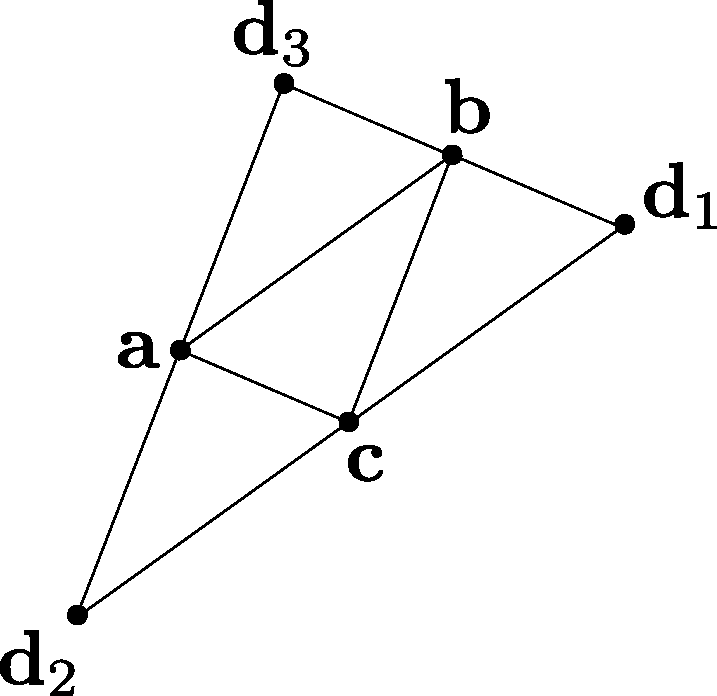
\includegraphics[width=1.5in]{figures/three_classes.pdf}
  \caption{The three equivalence classes: $A(\mathbf{a}, \mathbf{b},
  \mathbf{c}, \mathbf{d}_1), A(\mathbf{a}, \mathbf{b}, \mathbf{d}_2,
  \mathbf{c})$ and $A(\mathbf{a}, \mathbf{c}, \mathbf{d}_3,\mathbf{b})$.}
\label{FIG:3_classes}
\end{figure}

Let us mention an important point: if $a, b, c, d$ are not all distinct, the
equivalence classes contain less than $8$ proportions. This is natural,
because there are no longer $24$ different orderings of $a, b, c, d$. For
example if $a = c$ and $b = d$, then the equivalence class that is generated by
$A(a, b, c, d)$ is only made of $4$ proportions:
$$A(a, b, c, d) \eqdef A(a, b, a, b) \iff A(a, a, b, b) \iff A(b, b, a, a) \iff
(b, a, b, a).$$

Although these notions may seem shallow at first sight, they will actually turn
out to be paramount to grasp the geometrical view of Boolean proportions that
we now address.

\subsection{The Boolean and arithmetic proportions as parallelograms}

What we know so far is that the arithmetic proportion in $\mathbb{R}^m$
involves the four vertices of a parallelogram. As for the Boolean proportion,
we know from Definition \ref{DEF:analogy_for_vectors} that four Boolean vectors
$\mathbf{a}, \mathbf{b}, \mathbf{c}, \mathbf{d}$ are in proportion if each
component build up a valid proportion, i.e. that each of the $(a_i, b_i, c_i,
d_i)$ follow one of the $6$ valid patterns of Table
\ref{TAB:six_valid_patterns} on page \pageref{TAB:six_valid_patterns}.
\begin{testexample}
For example in $\mathbb{B}^2$, the four vectors $\mathbf{a} = (0, 0),~
  \mathbf{b} = (1, 0),~ \mathbf{c} = (0, 1)$ and $\mathbf{d} = (1, 1)$ are in
  proportion because the two component-wise proportions $a_1 : b_1 :: c_1 :
  d_1$ and $a_2 : b_2 :: c_2:d_2$ are valid: we have $0: 1 :: 0: 1$ and
  $0:0::1:1$.

  The four vectors $\mathbf{a} = (0, 0),~ \mathbf{b} = (1, 0),~ \mathbf{c} =
  (0, 1)$ and $\mathbf{d} = (1, 0)$ are \textbf{not} in proportion because $a_2
  : b_2 :: c_2 : d_2$ is not a valid pattern.
\end{testexample}

We have also seen that in $\mathbb{B}$, the Boolean
proportion and the arithmetic proportion are equivalent. This is also naturally
the case in $\mathbb{B}^m$! This means that a proportion in $\mathbb{B}^m$ can
also be represented as a (potentially \textit{flat}) parallelogram. By
\textit{flat} parallelogram we mean that the four vertices are not all
distinct: this will all become clear by looking at the two following
illustrations, in $\mathbb{B}^2$ and in $\mathbb{B}^3$.

\paragraph{The $36$ proportions of $\mathbb{B}^2$\\}

Figure \ref{FIG:proportions_in_B2} illustrates the proportions that
one can build in $\mathbb{B}^2$:
\begin{itemize}
  \item The proportion $\mathbf{a}: \mathbf{b} :: \mathbf{c} : \mathbf{d}$ and
    its 7 other equivalent forms, making up the parallelogram
    $\mathbf{a}\mathbf{b}\mathbf{c}\mathbf{d}$ (remember that when all elements
    are distinct, the equivalence class represented by $A(\mathbf{a},
    \mathbf{b}, \mathbf{c}, \mathbf{d})$ is composed of $8$ elements).
  \item The proportions that we can build using any pair of vertices, for
    example $\mathbf{a} : \mathbf{d} :: \mathbf{a} : \mathbf{d}$. Each of these
    proportions has $3$ other equivalent forms: in this case $\mathbf{a} :
    \mathbf{a} :: \mathbf{d} : \mathbf{d}$, $\mathbf{d} : \mathbf{a} ::
    \mathbf{d} : \mathbf{a}$ and $\mathbf{d} : \mathbf{d} :: \mathbf{a} :
    \mathbf{a}$. As there are $\binom{4}{2} = 6$ pairs of vertices in
    $\mathbb{B}^2$, there are exactly $6 \times 4$ proportions of this kind,
    all of which are flat\footnote{The \textit{flat} proportion are those that make
    up flat parallelograms. This naming convention is actually fortunate,
    because these proportions are in practice absolutely useless, as it will
    soon become clear in the next section.}.
  \item The $4$ proportions involving each vertex independently, for example
    $\mathbf{b}:\mathbf{b}::\mathbf{b}:\mathbf{b}$. These proportions are also
    flat, naturally.
\end{itemize}

\begin{figure}[!h]
\centering
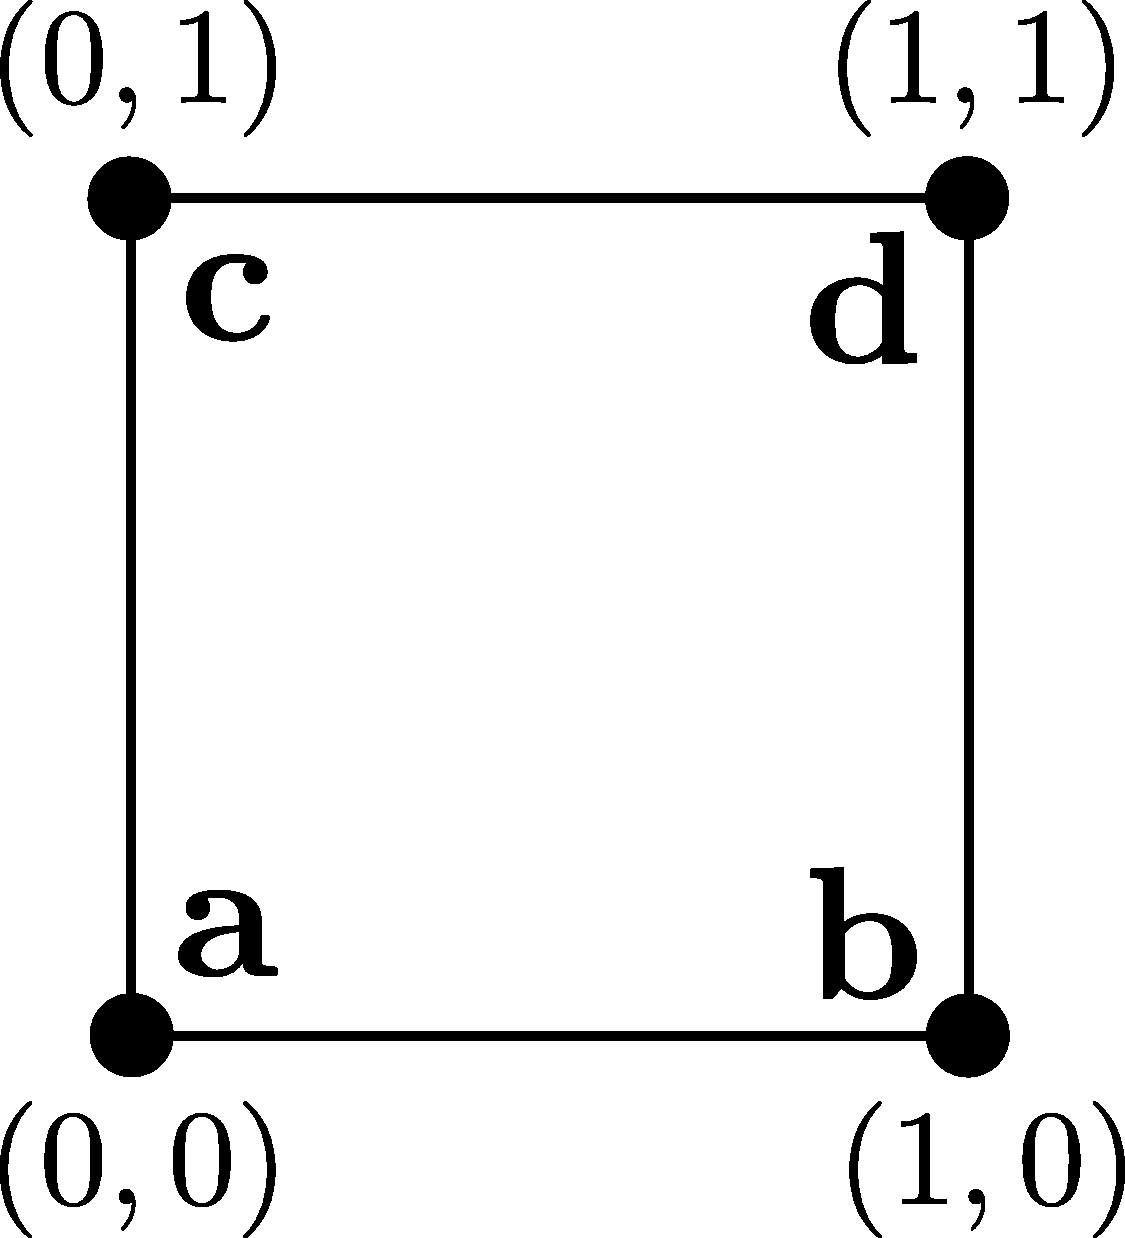
\includegraphics[width=1.5in]{figures/proportions_in_B2.pdf}
  \caption{The $36$ proportions in $\mathbb{B}^2$.}
\label{FIG:proportions_in_B2}
\end{figure}

All in all, this makes up to $36 = 8 + 6 \times 4 + 4$ proportions: $8$
proportions from the parallelogram $\mathbf{a}\mathbf{b}\mathbf{c}\mathbf{d}$,
$6 \times 4$ proportions from the pairs of vertices, and $4$ proportions from the
$4$ vertices. In fact, this number of $36$ proportions could have been derived
directly by remembering that in $\mathbb{B}^2$ the proportions are defined in a
component-wise fashion, and that there are exactly $6$ valid patterns of
proportions in $\mathbb{B}$: as a proportion in $\mathbb{B}^2$ is the
concatenation of two proportions in $\mathbb{B}$, the number of valid
proportions in $\mathbb{B}^2$ necessarily is $6 \times 6 = 36$.

Let us also note though that only $1 + 6 + 4 = 11$ of them can be considered
\textit{unique} (up to equivalence) and only one is non-flat. In the next
section, we will further investigate the number of unique proportions that can
be built in $\mathbb{B}^m$.

\paragraph{The proportions of $\mathbb{B}^3$\\}

Going a dimension further can still be insightful. Figure \ref{FIG:cubes_in_B3}
illustrates the 12 non-flat proportions that exist in $\mathbb{B}^3$. These
proportions are the parallelograms making up the 6 faces of the $3$-cube, and
six other \textit{diagonal} parallelograms passing through the center of the
cube.  The flat proportions are not shown for the sake of clarity.

\begin{figure}[!h]
\centering
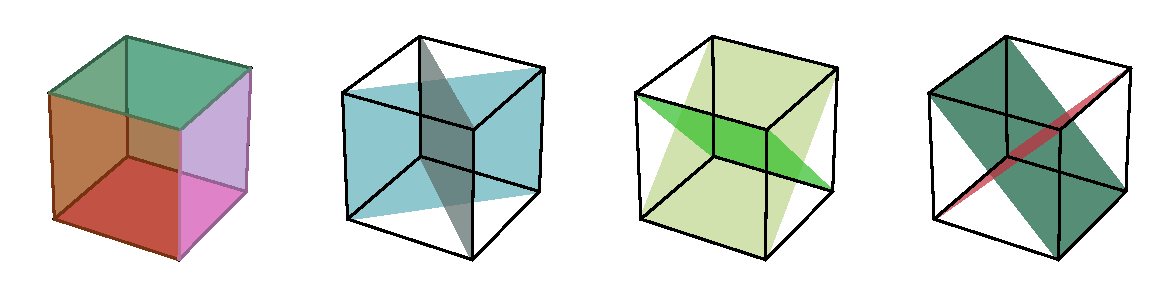
\includegraphics[width=\linewidth]{figures/cubes_in_B3.pdf}
  \caption{The $12$ \textit{non-flat} parallelograms in $\mathbb{B}^3$: the
  six faces of the cube, and $3 \times 2$ \textit{diagonal} parallelograms,
  e.g. $(000) : (010) :: (101) : (111)$.}
\label{FIG:cubes_in_B3}
\end{figure}

Let us finally note the following remarkable property, which will be useful to
us much later in Chapter \ref{CHAP:analogy_preserving_functions}:

\begin{property}
  \label{PROPER:hamming_distance_boolean_proportion}
  Let $\mathbf{a}, \mathbf{b},\mathbf{c}, \mathbf{d}$ in $\mathbb{B}^m$, and
  let $H(\mathbf{x}, \mathbf{x'})$ be the Hamming distance between $\mathbf{x}$
  and $\mathbf{x'}$, i.e. the number of components we need to flip to transform
  $\mathbf{x}$ into $\mathbf{x'}$ (or the reverse).\\
  If $\mathbf{a} : \mathbf{b}
  :: \mathbf{c} : \mathbf{d}$, then these three equalities hold:

  $$
  \begin{cases}
    H(\mathbf{a}, \mathbf{b}) = H(\mathbf{c}, \mathbf{d})\\
    H(\mathbf{a}, \mathbf{c}) = H(\mathbf{b}, \mathbf{d})\\
    H(\mathbf{a}, \mathbf{d}) = H(\mathbf{b}, \mathbf{c}).
  \end{cases}
  $$
\end{property}

We can easily verify this property in $\mathbb{B}$ from Table
\ref{TAB:six_valid_patterns}, and the general case in $\mathbb{B}^m$ immediately
follows from Definition \ref{DEF:analogy_for_vectors}. Sadly, Property
\ref{PROPER:hamming_distance_boolean_proportion} only offers a necessary
condition for a proportion to hold, and not a sufficient one: indeed taking $a
= d = 1$ and $b = c =0$ in $\mathbb{B}$, the three equalities are clearly
respected but $1:0::0:1$ is not a valid proportion. The first two
properties $H(\mathbf{a}, \mathbf{b}) = H(\mathbf{c}, \mathbf{d})$ and
$H(\mathbf{a}, \mathbf{c}) = H(\mathbf{b}, \mathbf{d})$ are classical
properties for parallelograms, but interestingly the third one $H(\mathbf{a},
\mathbf{d}) = H(\mathbf{b}, \mathbf{c})$ is only true for rectangles. In fact,
the parallelograms that we can build in $\mathbb{B}^m$ are \textbf{always}
rectangles.

This closes this discussion on the geometric interpretation of Boolean
proportions. In the next section we will apply the previously described notions
to a task of classification, which will help us to introduce new concepts, and
also to make a smooth transition towards the next chapter.

\section{Analogical inference principle and equation solving}
\label{SEC:machine_learning_with_boolean_proportions}

The goal of this last section is to introduce two other fundamental notions
that will be used in our investigations: the \textbf{analogical inference
principle}, and the process of \textbf{analogical equation solving}. Once
combined, these two concepts allow us to perform inference, and to apply
analogical reasoning to machine learning tasks such as classification.

We will here consider a toy classification problem in a Boolean setting, which
will help up introduce these two fundamental notions. This toy problem will
also serve as an introduction to the next chapter, where we will study the
theoretical properties of analogical classifiers. Because of the nature of the
problem, this section will be a mix of particular and general considerations.

\paragraph{Problem setting\\}

We now have enough background on Boolean proportions to start doing some
machine learning. Here is our problem. We consider the set $\mathbb{B}^m$ and
its $2^m$ elements. For various $\mathbf{x} \in \mathbb{B}^m$, we know the
value of $f(\mathbf{x})$, where $f$ is a function from $\mathbb{B}^m$ to
$\mathbb{B}$.  The value $f(\mathbf{x})$ is called the \textbf{class} of
$\mathbf{x}$, or its \textbf{label}. The set $S \subsetneq \mathbb{B}^m$ of
elements for which $f(\mathbf{x})$ is known is called the \textbf{training
set}. For any element $\mathbf{x} \notin S$, $f(\mathbf{x})$ is unknown and our
goal is to guess it: this is a binary \textbf{classification problem}.

Suppose we're in $\mathbb{B}^3$ and consider Figure
\ref{FIG:classification_problem}.
\begin{figure}[!h]
\centering
  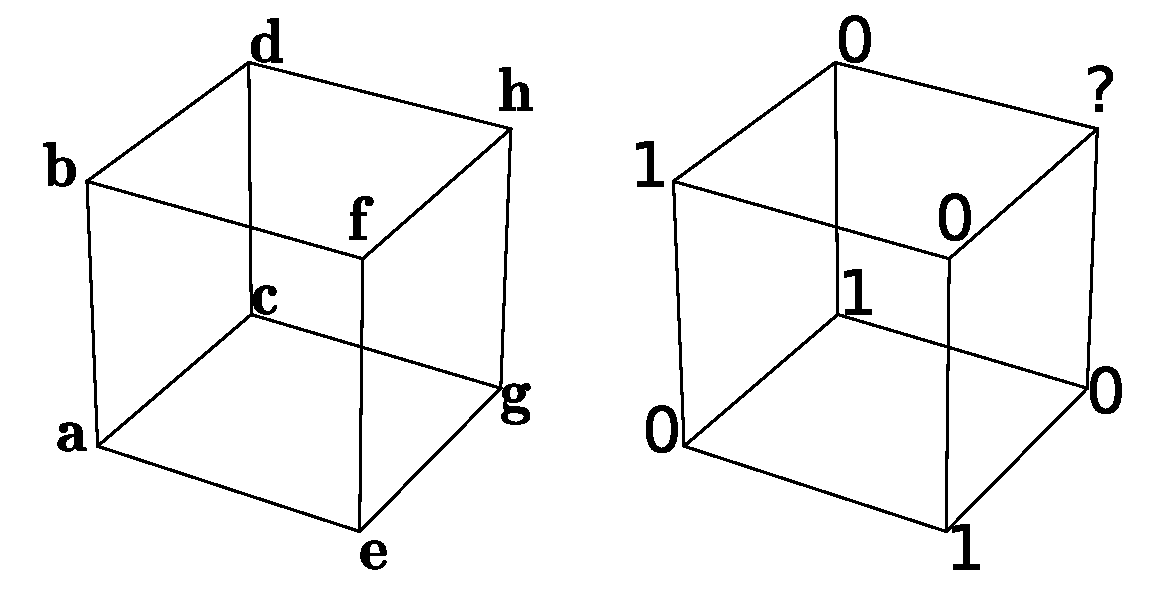
\includegraphics[width=3in]{figures/classification_problem.pdf}
  \caption{A classification problem in $\mathbb{B}^3$. Labels $f(\mathbf{x})$
  are on the right cube.}
\label{FIG:classification_problem}
\end{figure}
We know the values of $f(\mathbf{x})$ for
every single element $\mathbf{x}$ but $\mathbf{h}$, so $S = \{ \mathbf{a}, \mathbf{b},
\mathbf{c}, \mathbf{d}, \mathbf{e}, \mathbf{f}, \mathbf{g}\}$. There are
numerous methods at hand to go guess the value of $f(\mathbf{h})$. One of the
most famous one is the nearest neighbors heuristic, which would lead us to
consider that the label of $\mathbf{h}$ is the same as  that of its
\textit{neighbors}, i.e. the elements that are close to $\mathbf{h}$ with
respect to a given distance function. Using the Hamming distance, we would
assign to $\mathbf{h}$ the label $0$, because the $3$ closest neighbors of
$\mathbf{h}$, namely $\mathbf{d}, \mathbf{f}, \mathbf{g}$, are all labeled with
$0$.

\paragraph{The analogical inference principle\\}

Our point is here to describe the process of analogical classification, so we
will forget the nearest neighbor heuristic and we will instead make use of the
so-called \textbf{analogical inference principle}, which states that if four
elements $\mathbf{x}, \mathbf{y}, \mathbf{z}, \mathbf{t}$ are in proportion,
then their labels should also be in proportion:
$$
\infer[\text{Analogical inference principle}]{\mathbf{x} : \mathbf{y} ::
\mathbf{z} : \mathbf{t}}{f(\mathbf{x}) : f(\mathbf{y}) :: f(\mathbf{z}) :
f(\mathbf{t})}
$$

This is obviously an unsound principle, in that the conclusion does not
logically follows from the premise. But as we will see in this document, it can
still be useful.

The key point here is that if the value of $f(\mathbf{t})$ is unknown, it can
be \textbf{recovered} from the values of $f(\mathbf{x}), f(\mathbf{y}),
f(\mathbf{z})$ by the process of \textbf{analogical equation solving} that we
explain now.

We here want to guess the
value of $f(\mathbf{h})$. The analogical inference principle leads us to look
for all 3-tuples $(\mathbf{x}, \mathbf{y}, \mathbf{z}) \in S^3$ such that
$\mathbf{x}:\mathbf{y}::\mathbf{z}:\mathbf{h}$ holds.  The principle then states that
for all of these $3$-tuples, we should have
$f(\mathbf{x}):f(\mathbf{y})::f(\mathbf{z}):f(\mathbf{h})$.
Figure \ref{FIG:cubes_in_B3} tells us that there are 6 (non-flat)
parallelograms involving $\mathbf{h}$ as a vertex. The six unique corresponding
proportions are:

\begin{enumerate}
  \item $\mathbf{a} : \mathbf{b} :: \mathbf{g} : \mathbf{h}$
  \item $\mathbf{a} : \mathbf{d} :: \mathbf{e} : \mathbf{h}$
  \item $\mathbf{a} : \mathbf{c} :: \mathbf{f} : \mathbf{h}$
  \item $\mathbf{b} : \mathbf{d} :: \mathbf{f} : \mathbf{h}$
  \item $\mathbf{e} : \mathbf{f} :: \mathbf{g} : \mathbf{h}$
  \item $\mathbf{c} : \mathbf{g} :: \mathbf{d} : \mathbf{h}$
\end{enumerate}

Applying the analogical inference principle to the first proportion $\mathbf{a}
: \mathbf{b} :: \mathbf{g} : \mathbf{h}$ leads to $f(\mathbf{a}) :
f(\mathbf{b}) :: f(\mathbf{g}) : f(\mathbf{h})$, which is equivalent to:
$$0:1::0:f(\mathbf{h}).$$ By referring to Table \ref{TAB:six_valid_patterns} on
page \pageref{TAB:six_valid_patterns}, we
notice that $f(\mathbf{h})$ should be equal to $1$ for the proportion
$f(\mathbf{a}) : f(\mathbf{b}) :: f(\mathbf{g}) : f(\mathbf{h})$ to be a valid
one, because $0:1::0:1$. So we keep $1$ in the back of our head as a possible
candidate for $f(\mathbf{h})$: we say that $1$ is a \textbf{candidate
solution} for $f(\mathbf{h})$.  What we have just done is the \textbf{solving
of an analogical equation}.

\paragraph{Analogical equation solving in general\\}

Generally speaking, an analogical equation is a proportion $a:b::c:x$ in a
context where $x$ is unknown. Determining the value of $x$ is then called the
\textit{solving} of this equation. Depending on the nature and values of $a, b$,
and $c$, there may or may not exist a solution, and it might not be unique.

In fact, we have all been solving analogical equations since our childhood,
because in the case of the geometric proportion it reduces to the well known
rule of three: $\frac{5}{2} = \frac{10}{x} \implies x = \frac{2 \times 10}{5} =
4$, and generally $a:b::c:x \implies x = \frac{b \times c}{a}$ ($a \neq 0$).
The solution of the arithmetic proportion $a - b = c -x$ is also extremely
simple and is given by $x = c - a + b$.

In a Boolean setting, an equation is solvable for 6 patterns of $a, b, c$ (the
6 patterns of Table \ref{TAB:six_valid_patterns}, naturally):
\begin{proposition}
  \label{PROPOS:equation_solving}
  Let $a, b, c$ in $\mathbb{B}$. The analogical equation
  $a :b::c:x$
  is solvable if and only if $a = b$ or $a = c$. The solution denoted
  $\emph{sol}(a, b, c)$ is always unique and is given by:
  $$
  \begin{cases}
    \emph{sol}(a, b, c) \eqdef c \emph{~~ if } a = b,\\
    \emph{sol}(a, b, c) \eqdef b \emph{~~ if } a = c,
  \end{cases}
  $$
  or more generally:
  $$\emph{sol}(a, b, c) \eqdef c - a + b,$$
  because the Boolean proportion is a particular case of the arithmetic
  proportion. The values of $\emph{sol}(a, b, c)$ for all the Boolean $3$-tuples $(a,
  b, c)$ are given in Table \ref{TAB:solutions}.
\end{proposition}

\begin{table}[t]
  \centering
  \begin{tabular}[t]{cccc}
    \toprule
    $a$ & $b$ & $c$ & $\sol(a, b, c)$ \\
    \midrule
    0 & 0 & 0 & 0 \\
    1 & 1 & 1 & 1 \\
    0 & 0 & 1 & 1 \\
    1 & 1 & 0 & 0 \\
    0 & 1 & 0 & 1 \\
    1 & 0 & 1 & 0 \\
    1 & 0 & 0 &?\\
    0 & 1 & 1 &?\\
    \bottomrule
  \end{tabular}
  \caption{The solutions $\sol(a, b, c)$ for every Boolean $3$-tuple $(a, b,
  c)$. The question mark $?$ means that $\sol(a, b, c)$ is undefined. We can
  verify that $\sol(a, b, c) = c - a + b$ when the solution is defined.}
  \label{TAB:solutions}
\end{table}

\paragraph{Back to the estimation of $f(\mathbf{h})$\\}

Let's get back to the estimation of $f(\mathbf{h})$. Applying the analogical
inference principle to the second proportion $\mathbf{a} : \mathbf{d} ::
\mathbf{e} : \mathbf{h}$ leads $f(\mathbf{a)} : f(\mathbf{d}) :: f(\mathbf{e})
: f(\mathbf{h})$, and to the solving of $0:0::1:f(\mathbf{h})$. Here again, the
solution is $1$, just like the candidate of the first proportion.
The third proportion  $\mathbf{a} : \mathbf{c} :: \mathbf{f} : \mathbf{h}$
leads to the solving of $0:1::0:f(\mathbf{h})$, also claiming that $1$ is a good candidate.

And now the fourth proportion $\mathbf{b} : \mathbf{d} :: \mathbf{f} :
\mathbf{h}$, which leads to $1:0::0:f(\mathbf{h})$. \textbf{This equation is not
solvable}: neither $1:0::0:1$ nor $1:0::0:0$ are valid proportions. We can also
check this fact from Table \ref{TAB:solutions}. We thus
simply discard the proportion $\mathbf{b} : \mathbf{d} :: \mathbf{f} :
\mathbf{h}$ as a potential source of information about $f(\mathbf{h)}$, because
we are not in a position to apply the analogical inference principle. We can
easily verify that the fifth and sixth proportions also lead to non-solvable
equations.

All in all, we are left with three candidates coming from the first three
proportions, all of which are equal to $1$. Our guess will thus be that
$f(\mathbf{h})$ should be equal to $1$, so we will set the \textbf{estimation} of
$f(\mathbf{h})$ as $\hat{f}(\mathbf{h}) = 1$.
Notice that we have so far completely ignored  all the flat proportions,
i.e. proportions where the four elements are not all distinct.
This is because none of these proportions allow us to derive a solvable
equation. Considering for example $\mathbf{d} : \mathbf{h} :: \mathbf{d} :
\mathbf{h}$, we're led to the solving of $f(\mathbf{d}) : f(\mathbf{h}) ::
f(\mathbf{d}) : f(\mathbf{h})$, or equivalently of $0 : f(\mathbf{h}) :: 0 :
f(\mathbf{h})$. Both values $0$ and $1$ could lead to equally valid proportions
here, so there is simply no predictive power in the flat proportions. We have
also only considered unique proportions, up to equivalence. The first proportion
$\mathbf{a} : \mathbf{b} :: \mathbf{g} : \mathbf{h}$ for example is equivalent
to $\mathbf{a} : \mathbf{g} :: \mathbf{b} : \mathbf{h}$ (using central
permutation), which we could have
used instead. As any two equivalent proportions lead to the same solution for
their associated class equations, we usually choose to ignore all other equivalent
proportions, which allows to divide the number of equation solving processes by
a factor of $2$.

\paragraph{The analogical classification process: summary\\}

Here is a small outline of the classification process we have just followed,
that was entirely governed by the analogical inference principle. Our goal was
to guess the value of $f(\mathbf{h})$:

\begin{itemize}
  \item We first looked at all the $3$-tuples $(\mathbf{x}, \mathbf{y}, \mathbf{z}) \in
    \mathbf{B}^3$ such that:
    \begin{itemize}
      \item $f(\mathbf{x}), f(\mathbf{y})$ and $f(\mathbf{z})$ are known ;
      \item $\mathbf{x}:\mathbf{y}::\mathbf{z}:\mathbf{h}$ holds ;
      \item the \textbf{class equation} $f(\mathbf{x}) :f(\mathbf{y}) ::
        f(\mathbf{z}) :s$ is \textbf{solvable}. $s$ is called a
        \textbf{candidate solution}.
    \end{itemize}
    Each of the three candidate solutions $s_1, s_2, s_3$ agreed on the same prediction:
    $s_i = 1$ for all $i$.
  \item We thus estimated that $f(\mathbf{h})$ should indeed be equal to $1$.
\end{itemize}

\paragraph{Open questions\\}

This minimal example of analogical classification raises a few concerns, which
will be thoroughly addressed in the rest of this document:
\begin{enumerate}
  \item All of the three candidate solutions for $f(\mathbf{h})$ agreed on the
    same prediction: $1$. What if one of them predicted $0$? A first drastic
    option is to refuse to classify $\mathbf{h}$, on the basis that if the
    candidates cannot agree on their predictions, then we should not trust any
    of them. As it will become clear, in practice the candidates never really
    completely agree, even though sometimes a clear majority emerges. So this
    strategy would make the prediction impossible for most elements $\mathbf{x}
    \notin S$. A wiser option is to consider an aggregation of the candidate
    solutions: the most common one, for example. This is the option that has
    been taken on so far, as we will see in the next chapter.
  \item Here, by chance, the set of candidate solutions for $f(\mathbf{h})$ was
    not empty: we found three candidate solutions. What happens if we cannot
    find any candidate? This case arises when there are no 3-tuple
    $(\mathbf{x}, \mathbf{y}, \mathbf{z}) \in S^3$ such that $\mathbf{x} :
    \mathbf{y}::\mathbf{z}:\mathbf{h}$ holds and such that the associated equation
    $f(\mathbf{x}):f(\mathbf{y})::f(\mathbf{z}):f(\mathbf{h})$ is solvable. In
    the works of Stroppa and Yvon (\cite{StrYvoCNLL05}), such an $\mathbf{h}$
    cannot be classified. The notion of \textbf{analogical dissimilarity} as
    used in \cite{BayMicDelIJCAI07} will allow to bypass this issue. In the
    next chapter, we will detail these two versions of analogical learning, and
    one of the contributions of our work is to provide a unifying view of the
    two techniques.
  \item We have entirely relied on the analogical inference principle to
    classify $f(\mathbf{h})$. How \textit{safe} is this inference principle?
    Can we find some theoretical guarantees that could allow us to use it on a
    sound basis? In Chapter \ref{CHAP:analogy_preserving_functions}, we
    will provide a complete characterization of the Boolean functions $f$ that
    allow to derive sound conclusions.
\end{enumerate}

Before moving further to the next section, let us  consider a seemingly trivial
question: how many proportions can we build in $\mathbb{B}^m$? As we will see,
this question will provide us with some further insight about the Boolean proportion.
This last discussion is, however, not as important as the previous ones and can
safely be ignored by the impatient reader.

\paragraph{How many proportions can we build in $\mathbb{B}^m$?\\}
\label{SEC:number_of_parallelograms_in_Bm}

Exactly $6^m$! And it is fairly easy to derive: there are $6$ proportions in
$\mathbb{B}$. As a proportion in $\mathbb{B}^2$ is the concatenation of any two
proportions in $\mathbb{B}$, there are exactly $6^2 = 36$ proportions in
$\mathbb{B}^2$, as seen in the previous section. Analogical proportions in
$\mathbb{B}^m$ are defined component-wise, i.e. they are the concatenation of
$m$ proportions in $\mathbb{B}$. Equivalently, a proportion in $\mathbb{B}^m$
is the concatenation of a proportion in $\mathbb{B}^{m - 1}$ and a proportion
in $\mathbb{B}$. By trivial induction, we can build $6^m$ proportions in
$\mathbb{B}^m$.

But let's now ask a more relevant and challenging question: \textbf{how many
\textit{useful} proportions can we build in $\mathbb{B}^m$?} By
\textit{useful}, we mean proportions that could be used for classification
purposes.  We have seen in this section that the only proportions
$\mathbf{a} : \mathbf{b} :: \mathbf{c} : \mathbf{d}$ that are useful for
classification purposes are those where all elements $\mathbf{a}, \mathbf{b},
\mathbf{c}, \mathbf{d}$ are distinct, i.e. the non-flat proportions. We thus
want to exclude from the $6^m$ proportions those that comply with one of the
following patterns:

\begin{itemize}
  \item $\mathbf{a}: \mathbf{a} :: \mathbf{a} : \mathbf{a}$ ;
  \item $\mathbf{a}: \mathbf{b} :: \mathbf{a} : \mathbf{b}$, and its three
    equivalent forms $\mathbf{a}: \mathbf{a} :: \mathbf{b} : \mathbf{b}$,~
    $\mathbf{b}: \mathbf{a} :: \mathbf{b} : \mathbf{a}$, and $\mathbf{b}:
    \mathbf{b} :: \mathbf{a} : \mathbf{a}$.
\end{itemize}

Now, let's count them.

\begin{itemize}
  \item Each of the $2^m$ vertices $\mathbf{a}$ will generate a proportion of the
    form $\mathbf{a}: \mathbf{a} :: \mathbf{a} : \mathbf{a}$, so there are
    exactly $2^m$ proportions of this kind.
  \item Every pair $(\mathbf{a}, \mathbf{b})$ of vertices will generate four
    proportions:
    \begin{itemize}
      \item $\mathbf{a}: \mathbf{b} :: \mathbf{a} : \mathbf{b}$ ;
      \item $\mathbf{a}: \mathbf{a} :: \mathbf{b} : \mathbf{b}$ ;
      \item $\mathbf{b}: \mathbf{a} :: \mathbf{b} : \mathbf{a}$ ;
      \item $\mathbf{b}: \mathbf{b} :: \mathbf{a} : \mathbf{a}$.
    \end{itemize}
    There are $\binom{2^m}{2}$ distinct pairs of vertices, so in total this
    makes $4\cdot \binom{2^m}{2}$ proportions of the form $\mathbf{a}: \mathbf{b} ::
    \mathbf{a} : \mathbf{b}$ with its equivalent forms.
\end{itemize}

We are then left with the number of $6^m - 2^m - 4\cdot\binom{2^m}{2}$ useful
proportions. We know that for each of these proportions, all elements
$\mathbf{a}, \mathbf{b}, \mathbf{c}, \mathbf{d}$  are distinct. For each of
them, there are thus 7 other equivalent forms, which reduces the number of
useful and unique (up to equivalence) proportions to:
$$P_m = \frac{1}{8} \left[6^m - 2^m - 4\cdot\binom{2^m}{2} \right].$$
Table \ref{TAB:n_params_in_cube} gives the values of $P_m$ for the first $10$
values of $m$.
\begin{table}[h!]
\centering
  \begin{tabular}{ l  l }
\toprule
 $m$ & $P_m$\\
\midrule
    1	&	0\\
    2 &	1\\
    3	&	12\\
    4	&	100\\
    5 &	720\\
    6 &	4816\\
    7 &	30912\\
    8 &	193600\\
    9 & 1194240\\
    10 & 7296256\\
\bottomrule
\end{tabular}
\caption{Number of unique non-flat proportions in an $m$-dimensional cube.}
\label{TAB:n_params_in_cube}
\end{table}
Naturally, $P_2$ and $P_3$ are in accordance with the empirical  results from
Figures \ref{FIG:proportions_in_B2} and \ref{FIG:cubes_in_B3}. The fact that
$P_1 = 0$ means that no inference can be done with analogical proportion in
$\mathbb{B}$, which is perfectly normal: in $\mathbb{B}$, all proportions are
flat (i.e. the pattern is always $a:b::a:b$ or $a:a::b:b$).

In fact, it turns out that this sequence of numbers $0, 1, 12, 100\dots$ is
already known as the A016283 sequence from the OEIS\footnote{The On-line
Encyclopedia of Integer Sequences (\url{http://oeis.org/A016283})}.
This sequence actually describes \textit{the number of rectangles that can be
formed from the vertices of an $m$-dimensional cube}, which is exactly
equivalent to the number of \textit{useful} proportions that we wanted to
compute. The formula given by the OEIS is:
$$P_m = \frac{6^m}{8} - 4^{m - 1} + 2^{m - 3},$$
and using the fact that $\binom{n}{k} = \frac{n}{k}\binom{n - 1}{k - 1}$, it
can be shown that the two formulas $\frac{1}{8} \left[6^m - 2^m -
4\cdot\binom{2^m}{2} \right]$ and $\frac{6^m}{8} - 4^{m - 1} + 2^{m- 3}$ are,
fortunately, equivalent. It would be interesting to find out how the OEIS
formula was derived, but in all fairness we have no idea of the process that
was used.

\section*{Conclusion}

In this chapter, we have given the necessary background on formal analogical
proportions, mostly focusing on Boolean proportions. We have seen that an
analogical proportion $A$ is a quaternary relation following three simple
axioms that were already known in Aristotle times.

In the first section, we formally defined various analogical proportions in different settings,
starting from the most general definitions for semigroups and groups, until we
reached the Boolean proportion. We also presented an extension of the Boolean
proportion to multiple-valued logics, which we will use much later in Chapter
\ref{CHAP:analogical_recommendation}.

In the second section, we extended our knowledge and understanding of the Boolean
proportion. We illustrated the close bonds that exist between the Boolean
proportion and the arithmetic proportion, and we showed that both can be seen
as a relation between the four vertices of a parallelogram in $\mathbb{B}^m$ or
in $\mathbb{R}^m$.

The third section was devoted to the description of the analogical inference
principle and of the analogical equation solving process. By solving an
analogical equation, we are able to infer some information about any of the
four elements at play in an analogy, provided that the three others are known.
This process can be seen as a simple generalization of the rule of three that
we have been using since childhood: $\frac{4}{2} = \frac{6}{x} \implies x =
3$. Using this powerful tool and applying the analogical inference principle,
we were able to go trough a simple classification problem in a Boolean setting.

The aim of these first two chapters was to provide an overview of past works in
analogical reasoning, and to provide the necessary background to understand the
contributions made in this thesis. In the next chapter, we will describe our
contributions to the task of analogical classification.


\chapter{A functional definition of analogical classifiers}
\label{CHAP:functional_definition}
\localtableofcontents*
\vspace*{\baselineskip}

\initial{I}n Section \ref{SEC:machine_learning_with_boolean_proportions}, we
briefly described a basic process of analogical classification in an informal
way, making sure that everything went smoothly. In practice, bad things happen,
always. In this chapter, we will clearly and formally define analogical
classification, which will help us clarify some of the grey areas of Section
\ref{SEC:machine_learning_with_boolean_proportions}. Also (and most
importantly), we will describe our contributions to this problem.

A first form of analogical classifiers has been defined in the works of Stroppa
and Yvon \cite{StrYvoCNLL05}, which we will refer to as \textbf{conservative
classifiers}. Another form of analogical classifiers has later been proposed in
the works of Bayoudh, Delhay and Miclet \cite{MicBayDelJAIR08,
BayMicDelIJCAI07}, referred-to here as \textbf{extended classifiers}.

Though the theoretical groundings of the conservative and extended
classifiers have a lot in common (they are both analogical classifiers after
all), we will see that their practical implementation are actually quite
different. We will show however that the extended classifier is a
generalization of the conservative one, and most importantly that these two
approaches can be factorized into a single, unifying framework.

So far, only algorithmic descriptions of both methods were available. Our
unifying framework will allow us to give a general and \textbf{functional}
definition of analogical classifiers, opening the door to some theoretically
grounded research.

This chapter is structured as follows. In Section
\ref{SEC:analogical_classification}, we will review and detail the two previous
approaches to analogical classification, that we will name here the
conservative and the extended classifiers. We will se that these two approaches
can be factorized into a single functional description. Thanks to this
functional definition of analogical learners, we will be able in Section
\ref{SEC:theoretical_properties_of_analogical_classifiers} to derive some
theoretical properties about analogical learners. We will indeed show that
their VC-dimension is infinite, and that their accuracy is closely related to
that of the $k$-NN classifier. Finally in Section
\ref{SEC:experiments_and_empirical_validation}, we will empirically verify our
results and provide some insights that will motivate the topic of Chapter
\ref{CHAP:analogy_preserving_functions}.

\section{Analogical classification}
\label{SEC:analogical_classification}

This first section will be devoted to the unification of two seemingly
different analogical approaches to classification.  Let us first define the
problem of classification, one of the main subfields of machine learning. The
aim is simple: a classifier has to estimate the class of any element given as
input on the basis of some other elements for which the class is known.
Formally, we denote $X^m$ our universe which is usually a Cartesian product:
$X^m = X_1 \times X_2 \times \ldots \times X_m$. We have at our disposal a
subset $S \subsetneq X^m \times Y$ of $n$ pairs $\left(\mathbf{x},
f(\mathbf{x})\right)$, called the \textbf{training set}.  $$S=
\Set{\left(\mathbf{x}^{(i)}, f(\mathbf{x}^{(i)})\right) \in X^m \times Y | i
\in [1,n]}.$$

For any $\mathbf{x} \in X^m$, the value $f(\mathbf{x})$ is called its
\textbf{class} or \textbf{label}.
The functional notation $f(\mathbf{x})$ suggests that all labels
are defined by an underlying function $f \colon X^m \to Y$, which is the usual
general view point of machine learning. In the case of classification, $Y$ is a
finite set of size $C$ where $C$ is the number of different classes. The goal
of a classifier is to \textbf{learn} the function $f$ on the basis of the
elements in $S$, called the \textbf{examples}. The output of a classifier is a
function $\hat{f} \colon X^m \to Y$ that is \textit{as close as possible} the
ground truth function $f$.

\subsection{Conservative classifier}
\label{SEC:conservative_classifier}

We will here describe what we call a \textbf{conservative} classifier. Without
further ado, let us consider Algorithm \ref{ALGO:conservative_classifier} which
describes such classifiers.

\begin{algorithm}[!ht]
\caption{The Conservative classifier.}
\label{ALGO:conservative_classifier}
  \begin{algorithmic}
    \STATE {\bf Input}: A training set $S$ and an element $\mathbf{x} \in X^m
    \setminus S$ for which $f(\mathbf{x})$ is unknown.
    \STATE {\bf Output}: $\hat{f}(\mathbf{x})$, an estimation of
    $f(\mathbf{x})$.
    \STATE {\bf Init}: $\mathbf{C}(\mathbf{x}) = \varnothing$ \quad \quad // A multiset of candidate
    labels.

    \FORALL{$(\mathbf{a}, \mathbf{b}, \mathbf{c}) \in S^3$ such that
    $\mathbf{a} : \mathbf{b} :: \mathbf{c} : \mathbf{x}$}
    \IF{$f(\mathbf{a}) : f(\mathbf{b}) ::f(\mathbf{c}) : y$ is
    solvable}
    \STATE $y = \sol\left(f(\mathbf{a}), f(\mathbf{b}), f(\mathbf{c})\right)$
    \STATE $ \mathbf{C}(\mathbf{x}) = \mathbf{C}(\mathbf{x}) \cup y$
    \ENDIF
	  \ENDFOR
    \STATE $\hat{f}(\mathbf{x}) = \text{Mode} (\mathbf{C}(\mathbf{x}))$ // The most common value in
    $\mathbf{C}(\mathbf{x})$ (undefined if $\mathbf{C}(\mathbf{x}) = \varnothing$).
  \end{algorithmic}
\end{algorithm}

It should be easy to see that the process of Algorithm
\ref{ALGO:conservative_classifier} is extremely similar to the one we followed
on our first introduction to classification with Boolean proportions in
Section \ref{SEC:machine_learning_with_boolean_proportions}. Here again the key
underlying process is the analogical inference principle, which states that if
four elements are in proportion, then their classes should also be in
proportion. But Algorithm \ref{ALGO:conservative_classifier} is slightly more
general than what we have glimpsed in Section
\ref{SEC:machine_learning_with_boolean_proportions}: it allows to deal with
cases where some of the candidate solutions $y$ do not agree with each other.
The fix here is to consider that the prediction $\hat{f}(\mathbf{x})$ will be
the most common candidate solution among all the predictors. This definition of
analogical classification comes from the work of Stroppa and Yvon
\cite{StrYvoCNLL05, StrYvoREPORT05}, and to our knowledge it is the first
instance of analogical learner that has ever been proposed. We note however
that the authors did not explicitly state that the class equations must be
solvable to be useful.

Note that if the multiset $\mathbf{C}(\mathbf{x})$ is empty, i.e. if we cannot find
$3$-tuples in $S^3$ such that they are in proportion with $\mathbf{x}$ and such
that the related class equation is solvable, then the value
$\hat{f}(\mathbf{x})$  is undefined and $\mathbf{x}$ cannot be classified
(hence the name \textit{conservative}).

At first sight, we are here in a setting where the examples in $S$ are stored
for future use, without any generalization process.  We will thus consider (for
now) that the conservative classifier ranges among the category of
\textbf{lazy learners}, i.e. learners that only rely on the training set $S$
without any actual \textit{learning} stage, or without building any model of
the data. The most popular instance of lazy learner certainly is the famous
$k$-NN algorithm.

In the following, we will give a functional definition of $\hat{f}(\mathbf{x})$
as outputted by a conservative classifier. To this end, we will define two
crucial concepts: the \textbf{analogical extension} of a training set $S$, and
the \textbf{analogical root} of an element $\mathbf{x}$. Both the analogical
extension and the analogical root were first defined in \cite{StrYvoREPORT05},
with some minor differences with our definitions.

\begin{definition}[Analogical extension]
  \label{DEF:analogical_extension}
  Denoting $S$ a training set and $f$ the ground truth function of the labels,
  the \textbf{analogical extension} of $S$ using $f$ is:
  $$
  \esf \eqdef \Set{ \mathbf{x} \in X^m |  \exists
  (\mathbf{a},\mathbf{b},\mathbf{c}) \in S^3, ~ \mathbf{a} : \mathbf{b} ::
  \mathbf{c} : \mathbf{x} \text{ and } f(\mathbf{a}) : f(\mathbf{b}) ::
  f(\mathbf{c}) : y \text{ is solvable}}.
  $$
\end{definition}

Intuitively,  $\esf$ can be regarded as the set of all $\mathbf{x} \in X^m$
that are in proportion with at least one 3-tuple in $S$, provided that the
equation related to the associated labels is also solvable. For any $S$ and any
$f$, $\esf$ satisfies some interesting properties: \begin{enumerate}
\item $S \subseteq \esf$, since $\mathbf{x} : \mathbf{x} :: \mathbf{x}
  :\mathbf{x}$ always holds;
\item $\aext{\varnothing}{f} = \varnothing$, and $\aext{X^m}{f}=X^m$;
\item $S_1 \subseteq S_2 \implies \aext{S_1}{f} \subseteq \aext{S_2}{f}$.
\end{enumerate}
We will denote by $\esfs$ the set of elements in $\esf$ that are not in $S$:
$$\esfs \eqdef \esf \setminus S.$$ In a setting where for any
$\mathbf{a},\mathbf{b}, \mathbf{c}$ the equation $\mathbf{a} : \mathbf{b} ::
\mathbf{c} : \mathbf{x}$ is always solvable (as is the case for the arithmetic
proportion) and such that the associated class equation is also solvable, we
can show that the size of $\esfs$ is exactly $\frac{1}{2} n^2(n - 1)$. This
value is thus a loose upper bound for $\mid \esfs\mid$, because in practice
equations are not always solvable.

\begin{testexample}
To polish our understanding of the analogical extension, let us consider Figure
\ref{FIG:ae_example}.
The training set $S$ is $\Set{\mathbf{a}, \mathbf{b}, \mathbf{d},\mathbf{e}}$.
Taking $(\mathbf{b}, \mathbf{d}, \mathbf{a}) \in S^3$, we notice that
$\mathbf{b} : \mathbf{d} :: \mathbf{a} : \mathbf{c}$, and the associated class
equation $0:1::0:y$ is solvable. So $\mathbf{c}$ is in $\esf$. The same goes for
$\mathbf{f}$ with the 3-tuple $(\mathbf{a}, \mathbf{b}, \mathbf{e}) \in S^3$.
However, even if we can find $(\mathbf{b}, \mathbf{d}, \mathbf{e}) \in S^3$
such that $\mathbf{b} : \mathbf{d} :: \mathbf{e} : \mathbf{g}$, the associated
class equation $0:1::1:y$ is not solvable, so $\mathbf{g} \notin \esf$. At
last, vertex $\mathbf{h}$ will suffer the same fate because the class equation
$f(\mathbf{a}) : f(\mathbf{e}) :: f(\mathbf{d}) : y$ is not solvable either. In
the end, $\esf = \set{\mathbf{a}, \mathbf{b}, \mathbf{c}, \mathbf{d},
\mathbf{e}, \mathbf{f}}$ and $\esfs = \Set{\mathbf{c}, \mathbf{f}}$.
\end{testexample}

\begin{figure}[!h]
\centering
  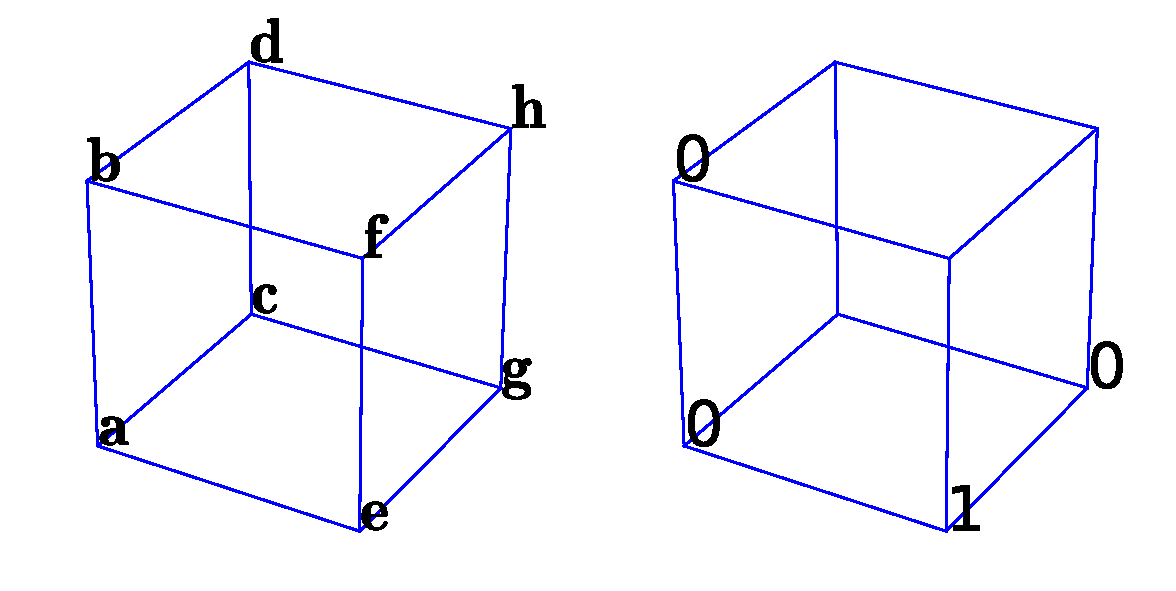
\includegraphics[width=3in]{figures/ae_example.pdf}
  \caption{With $S = \Set{\mathbf{a}, \mathbf{b}, \mathbf{d},
  \mathbf{e}}$, we have $\esfs = \Set{\mathbf{c}, \mathbf{f}}$.}
\label{FIG:ae_example}
\end{figure}

The dual concept of the analogical extension is what we call the
\textbf{analogical root} of a given element $\mathbf{x} \in X^m$:

\begin{definition}[Analogical root]
  \label{DEF:analogical_root}
  Denoting $S$ a training set and $f$ the ground truth function of the labels,
  the \textbf{analogical root} of an element $\mathbf{x} \in X^m$ is:
  $$
  \rsfx \eqdef \Set{(\mathbf{a}, \mathbf{b}, \mathbf{c}) \in S^3 |
  \mathbf{a}:\mathbf{b}::\mathbf{c}:\mathbf{x} \text{ and }
  f(\mathbf{a}):f(\mathbf{b})::f(\mathbf{c}):y \text{ is solvable}}.
  $$
\end{definition}

\noindent
$\rsfx$ is simply the set of 3-tuples in $S$ which are analogically linked to
$\mathbf{x}$.

\begin{testexample}
Considering again the example of Figure \ref{FIG:ae_example}, we have that
$\aroot{S}{f}{\mathbf{c}} = \Set{(\mathbf{b}, \mathbf{d},\mathbf{a}),
(\mathbf{b}, \mathbf{a},\mathbf{d})}$. However, the two corresponding
proportions $\mathbf{b}: \mathbf{d}::\mathbf{a}:\mathbf{c}$ and $\mathbf{b}:
\mathbf{a}::\mathbf{d}:\mathbf{c}$ are equivalent, and we will follow the
convention that the analogical root should only contain non-equivalent
3-tuples, so technically $\aroot{S}{f}{\mathbf{c}}$ is entirely described by
$\Set{(\mathbf{b}, \mathbf{d},\mathbf{a})}$.  We also have that
$\aroot{S}{f}{\mathbf{f}} = \Set{(\mathbf{a}, \mathbf{b},
\mathbf{e})}$, $\aroot{S}{f}{\mathbf{a}} = \Set{(\mathbf{a}, \mathbf{a},
\mathbf{a}), (\mathbf{b}, \mathbf{b}, \mathbf{a}), (\mathbf{d}, \mathbf{d},
\mathbf{a}), (\mathbf{e}, \mathbf{e}, \mathbf{a})}$, and
$\aroot{S}{f}{\mathbf{h}} = \varnothing$. \end{testexample}

It is clear that in general, $$\rsfx = \varnothing\iff \mathbf{x} \notin
\esf.$$ It should also be clear that even if we only consider unique 3-tuples
(up to equivalence) in the analogical root, $\rsfx$ may contain more than one
3-tuple: for example in $\mathbb{R}^m$ or $\mathbb{B}^m$ with the arithmetic
(or Boolean) proportion, $\mathbf{x}$ may be the involved in more than one
parallelogram, as illustrated in Figure \ref{FIG:multiple_parallelograms}.

\begin{figure}[!h]
\centering
  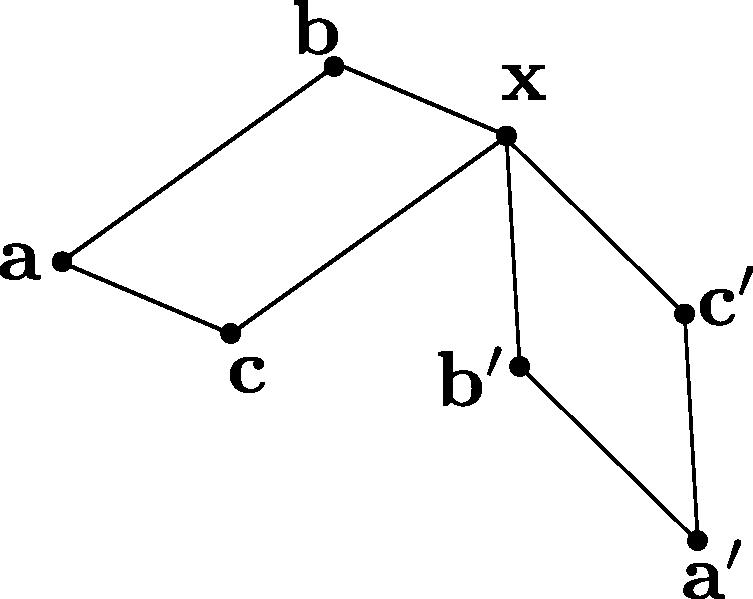
\includegraphics[width=2.5in]{figures/multiple_parallelograms.pdf}
  \caption{With $S = \Set{\mathbf{a}, \mathbf{b}, \mathbf{c}, \mathbf{a}',
  \mathbf{b}', \mathbf{c}'}$, we have $\mathbf{x} \in \esf$ and $\rsfx =
  \Set{(\mathbf{a}, \mathbf{b}, \mathbf{c}), (\mathbf{a}', \mathbf{b}',
  \mathbf{c}')}$. Class equations are all assumed to be solvable.}
\label{FIG:multiple_parallelograms}
\end{figure}

We need to introduce one last definition before we can go on with the
functional view of conservative classifiers:

\begin{definition}[Analogical label]
  \label{DEF:analogical_label}
  For any element $\mathbf{x}$ of $\esf$, we denote $\mathbf{C}(\mathbf{x})$
  the set of the class equations solutions associated with $\mathbf{x}$:
  $$\mathbf{C}(\mathbf{x}) \eqdef \Set{y | f(\mathbf{a}) : f(\mathbf{b}) ::
  f(\mathbf{c}) :y, \quad \text{with }(\mathbf{a}, \mathbf{b}, \mathbf{c}) \in \rsfx}$$
  We then define the \textbf{analogical
  label} of $\mathbf{x}$, denoted $\albl{\mathbf{x}}$, as:
  $$\albl{\mathbf{x}} \eqdef
  \begin{cases}
    f(\mathbf{x}) \text{ if } \mathbf{x} \in S\\
    \text{Mode} \left(\mathbf{C}(\mathbf{x})\right) \text{ if
    } x \notin S
  \end{cases}
  $$
  where $\text{Mode}(\mathbf{C})$ returns the most frequent element of the multiset
$\mathbf{C}$. In case of a tie, the returned element is chosen at random between
the most frequent elements.
\end{definition}

We are now in position to give a functional definition of the conservative
classifier:

\begin{definition}[Conservative classifier]
  \label{DEF:conservative_classifier}
  Given a training set $S$ with an underlying ground truth function $f$,
  a conservative classifier sets the prediction of an element $\mathbf{x}$ as
  follows:

  $$\text{If } \mathbf{x} \in \esf, ~ \hat{f}(\mathbf{x}) \eqdef \albl{\mathbf{x}}.
  \text{ Else, } \hat{f}(\mathbf{x}) \text{ is undefined.}$$
\end{definition}

As previously mentioned, a conservative classifier is not able to output a
prediction if $\mathbf{x}$ does not belong to the analogical extension. We have
already made this observation when describing Algorithm
\ref{ALGO:conservative_classifier}: for a given $\mathbf{x}$, the set of
candidate solutions $\mathbf{C}(\mathbf{x})$ is empty if and only if
$\mathbf{x} \notin \esf$.  Also, we now understand why $\albl{\mathbf{x}}$ is
simply set to $f(\mathbf{x})$ when the $\mathbf{x} \in S$: for such an
$\mathbf{x}$ it is natural to want $\hat{f}(\mathbf{x}) = f(\mathbf{x})$!

\begin{testexample}
Going
back to our example with Figure \ref{FIG:ae_example}, we will have
$\hat{f}(\mathbf{c}) \eqdef \albl{\mathbf{c}} = 1$, because
$\aroot{S}{f}{\mathbf{c}} = \Set{(\mathbf{b}, \mathbf{d},\mathbf{a})}$ and
$\mathbf{C}(\mathbf{c}) = \Set{1}$. Also, $\hat{f}(\mathbf{f}) \eqdef
\albl{\mathbf{f}} = 1$, because $\aroot{S}{f}{\mathbf{f}} =
\Set{(\mathbf{a},\mathbf{b},\mathbf{e})}$ and $\mathbf{C}(\mathbf{f}) =
\Set{1}$. Here, we did not need to use the majority vote procedure as there was
only one candidate solution for each prediction. As $\mathbf{g}$ and
$\mathbf{h}$ do not belong to $\esf$, both $\albl{\mathbf{g}}$ and
$\albl{\mathbf{h}}$ stay undefined.
\end{testexample}

Let us note that in Algorithm \ref{ALGO:conservative_classifier}, the
analogical extension $\esf$ is never explicitly computed. Instead, for a given
$\mathbf{x}$, we look for
every 3-tuple in $S^3$ and check if they belong to $\rsfx$. One drawback is
that the search in $S^3$ has to be done for every new element $\mathbf{x}$ that
we want to classify, and can prove to be quite expensive in computation time,
even for small sizes of $S$. However, taking advantage of our functional
definition, we can reformulate the learning process of a conservative
classifier as follow:

\begin{itemize}
\item First, compute $\esf$. While $\esf$ is begin computed, it is trivial to
  also compute the set of candidates $\mathbf{C}(\mathbf{x})$ for each $x \in
    \esf$.
  \item Then, for all $x \in\esf$, compute
    $\albl{\mathbf{x}} \eqdef \text{Mode}(\mathbf{C}(\mathbf{x}))$.
\end{itemize}
\noindent
Whenever we are asked to classify a given $\mathbf{x}$, all we need now is to
check whether $\mathbf{x}$ belongs to $\esf$ or not. The output
$\hat{f}(\mathbf{x})$ is then immediate. This way to proceed has the undeniable
advantage to perform the search in $S^3$ only once. Obviously, this saving in
computation time is done at the expense of memory consumption, because the
size of $\esf$ can be drastically greater than that of $S$. This alternative
view also leads us to reconsider our previous statement about conservative
classifiers belonging to the class of lazy learners. Here, the computation of
the analogical extension can be viewed as a generalization process, even if not
all elements of the universe $X^m$ are affected by this generalization.

We will end this Section on conservative classifier by sketching a use-case
described in \cite{StrYvoREPORT05}, where an analogical proportion is defined
on the set of words over a finite alphabet, and the task is to learn the
conjugation of English verbs. This setting is slightly different than that of
classification that we have settled-in, but all definitions and concepts remain
valid. Here, solving the analogical equation
$\text{view}:\text{reviewer}::\text{search}:y$ leads to $\text{researcher}$,
using the definition of the analogy and the concatenation operator.
We have a training set $S=\Set{\mathbf{x}^{(1)},\mathbf{x}^{(2)},
\mathbf{x}^{(3)}, \mathbf{x}^{(4)}, \mathbf{x}^{(5)}}$ where
$\mathbf{x}^{(1)}=(read,3,reads), \mathbf{x}^{(2)}=(read,G,reading),
\mathbf{x}^{(3)}=(view,3,views)$, $\mathbf{x}^{(4)}=(view,G,viewing),
\mathbf{x}^{(5)}=(eat,3,eats)$. $(read,3,reads)$ means that $read$ is
transformed into $reads$ when conjugated at the third person singular, and $G$
stands for the gerund form.

Given a new element $\mathbf{x}=(eat,G,y)$, $\rsfx=
\Set{\left(\mathbf{x}^{(1)}, \mathbf{x}^{(2)}, \mathbf{x}^{(5)}\right),
\left(\mathbf{x}^{(3)},\mathbf{x}^{(4)},\mathbf{x}^{(5)}\right)}$. The
prediction is as expected $\hat{f}(\mathbf{x})=\text{eating}$, which is the
solution of the equations $\text{read}:\text{reading}::\text{eat}:y$ and
$\text{view}:\text{viewing}::\text{eat}:y$. There is
no solution for $\mathbf{x}=(absurd,G,y)$, just because $\rsfx= \varnothing$.

The fact that conservative learners cannot output a prediction for any
$\mathbf{x}$ can here be considered a good thing: it would not be natural to
look for the gerund form of \textit{absurd}. However, in many use cases we do
want our classifier to be able to predict the label of any element. This is why
other options have been implemented to overcome this problem, and to extend in
some sense the generalization ability of analogical learners. This is the
purpose of \textbf{extended classifiers} described in the next section.

\subsection{Extended classifier}
\label{SEC:extended_classifier}

We now want our analogical classifier to be able to predict the label of any
input element $\mathbf{x} \in X^m$, and not just the ones in $\esf$.
The main bottleneck of Algorithm \ref{ALGO:conservative_classifier} is that we
require the 3-tuples in $S^3$ to be in perfect proportion with the element
$\mathbf{x}$ we want to classify. Such 3-tuples are not always available in the
training set, so necessarily some elements of $X^m$ are excluded from $\esf$.

The key concept that will help us overcome this issue is what we call an
\textbf{analogical dissimilarity}, first introduced in
\cite{BayMicDelIJCAI07}. The analogical dissimilarity is a measure that
quantifies in some sense \textit{how far} a relation $\mathbf{a} : \mathbf{b}
:: \mathbf{c} : \mathbf{d}$ is from being a perfectly valid proportion.

We keep the initial notation $\AD(\mathbf{a}, \mathbf{b},
\mathbf{c},\mathbf{d})$ to denote the analogical dissimilarity between 4
elements.  Some  minimal properties have to be satisfied by such a
dissimilarity $\AD \colon {(X^m)}^4 \longrightarrow \mathbb{R}^+$ to fit
with the intuition. For any $\mathbf{a}, \mathbf{b},\mathbf{c},\mathbf{d},
\mathbf{e}, \mathbf{f} \in X^m$, the following properties should hold:
\begin{itemize}
  \item $\AD(\mathbf{a}, \mathbf{b},\mathbf{c},\mathbf{d})=0 \iff \mathbf{a} :
    \mathbf{b}:: \mathbf{c} : \mathbf{d}$ (Consistency with the Analogy)
  \item $\AD(\mathbf{a}, \mathbf{b},\mathbf{c},\mathbf{d})=
    \AD(\mathbf{c}, \mathbf{d},\mathbf{a},\mathbf{b})$ (Symmetry)
  \item $\AD(\mathbf{a}, \mathbf{b},\mathbf{c},\mathbf{d})=
    \AD(\mathbf{a}, \mathbf{c},\mathbf{b},\mathbf{d})$ (Central permutation)
  \item $\AD(\mathbf{a}, \mathbf{b},\mathbf{e},\mathbf{f}) \leq \AD(\mathbf{a},
    \mathbf{b},\mathbf{c},\mathbf{d}) + \AD(\mathbf{c},
    \mathbf{d},\mathbf{e},\mathbf{f})$ (Triangle inequality)
  \item In general, $\AD(\mathbf{a}, \mathbf{b},\mathbf{c},\mathbf{d}) \neq
    \AD(\mathbf{b}, \mathbf{a},\mathbf{c},\mathbf{d})$
\end{itemize}
Naturally, the symmetry and central permutation properties lead to the same
three classes of equivalence that we have for the analogical proportion. In
particular, the equivalence class that is \textit{generated} by
$\AD(\mathbf{a}, \mathbf{b},\mathbf{c},\mathbf{d})$ is:
\begin{align*}
  &\AD(\mathbf{a}, \mathbf{b},\mathbf{c},\mathbf{d}) =
\AD(\mathbf{c}, \mathbf{d},\mathbf{a},\mathbf{b})=
\AD(\mathbf{c}, \mathbf{a},\mathbf{d},\mathbf{b})=
\AD(\mathbf{d}, \mathbf{b},\mathbf{c},\mathbf{a})=
\AD(\mathbf{d}, \mathbf{c},\mathbf{b},\mathbf{a})=\\
  &\AD(\mathbf{b}, \mathbf{a},\mathbf{d},\mathbf{c})=
\AD(\mathbf{b}, \mathbf{d},\mathbf{a},\mathbf{c})=
\AD(\mathbf{a}, \mathbf{c},\mathbf{b},\mathbf{d}).
\end{align*}

The definition of an analogical proportion strongly relies on the structure and
operators available on $X^m$, and the same goes for the definition of the
analogical dissimilarity: there are a lot of possibilities. For the arithmetic
proportion in $\mathbb{R}^m$, the analogical dissimilarity  $\AD(\mathbf{a},
\mathbf{b},\mathbf{c},\mathbf{d})$ should capture \textit{how far}
are $\mathbf{a}, \mathbf{b},\mathbf{c},\mathbf{d}$ from making up a perfect
parallelogram. This can be achieved using the following definition:

% Note: leave \emph{AD} here else it will be in italics.
\begin{definition}[Analogical dissimilarity for real vectors]
  \label{DEF:AD_arithmetic_proportion}
  Given four vectors $\mathbf{a}, \mathbf{b},\mathbf{c},\mathbf{d}$ of
  $\mathbb{R}^m$ equipped with the standard $p$-norm $\norm{p}{\cdot}$, the
  analogical dissimilarity related to the arithmetic proportion is defined as:
  $$\text{AD}(\mathbf{a}, \mathbf{b},\mathbf{c},\mathbf{d}) =
  \norm{p}{(\mathbf{a} - \mathbf{b}) - (\mathbf{c} - \mathbf{d})}.$$
\end{definition}

Of course, we will need an analogical dissimilarity in $\mathbb{B}^m$, but we
will start small and consider $\mathbb{B}$ first:
\begin{definition}[Analogical dissimilarity for Boolean vectors]
  \label{DEF:AD_boolean_proportion}
  Given four elements $a, b, c, d$ of $\mathbb{B}$, the analogical
  dissimilarity $\text{AD}(a, b, c, d)$ is defined as the number of values that
  have to be switched to get a proper analogy.
\end{definition}
\noindent
Table \ref{TAB:analogical_dissimilarity} shows the values of $\AD(a, b, c, d)$
for 8 patterns. The $8$ remaining patterns have the same values of $AD$ as
their negated versions and have thus been ignored.
\begin{table}[t]
  \centering
  $$
  \begin{array}{ccccc}
    \toprule
    a & b & c & d &  \AD(a, b, c, d)\\
    \midrule
    0 & 0 & 0 & 0 &   \textbf{0}\\
    0 & 1 & 0 & 1 &   \textbf{0}\\
    0 & 0 & 1 & 1 &   \textbf{0}\\
    0 & 0 & 0 & 1 &   \textbf{1}\\
    0 & 0 & 1 & 0 &   \textbf{1}\\
    0 & 1 & 0 & 0 &   \textbf{1}\\
    1 & 0 & 0 & 0 &   \textbf{1}\\
    0 & 1 & 1 & 0 &   \textbf{2}\\
    \bottomrule
  \end{array}
  $$
  \caption{The values of $\text{AD}(a, b, c,d)$ for eight patterns of $a, b, c,
  d$ in $\mathbb{B}$.}
  \label{TAB:analogical_dissimilarity}
\end{table}
The natural extension to $\mathbb{B}^m$ is again to consider component-wise
proportions. The analogical dissimilarity in $\mathbb{B}^m$ is thus defined as
the sum of the $m$ individual Add:
$$\AD(\mathbf{a}, \mathbf{b},\mathbf{c},\mathbf{d}) = \sum\limits_{i=1}^m
\AD(a_i,b_i,c_i,d_i).$$
We get an analogical dissimilarity whose co-domain is $[0, 2m]$. In fact, if we
use the $1$-norm defined as $\norm{1}{\mathbf{x}} = \sum_{i = 1}^m |x_i|$,
Definition \ref{DEF:AD_arithmetic_proportion} is equivalent to Definition
\ref{DEF:AD_boolean_proportion}. This means that for $\mathbf{a},
\mathbf{b},\mathbf{c},\mathbf{d}$ in $\mathbb{B}^m$, $\AD(\mathbf{a},
\mathbf{b},\mathbf{c},\mathbf{d}) =
\norm{1}{(\mathbf{a}-\mathbf{b})-(\mathbf{c}-\mathbf{d})}$. Note that the
expression $\norm{1}{(\mathbf{a}-\mathbf{b})-(\mathbf{c}-\mathbf{d})}$ is
nothing but the Hamming distance between the two vectors
$(\mathbf{a}-\mathbf{b})$ and $(\mathbf{c}-\mathbf{d})$\footnote{$\mathbb{B}^m$
is not closed under addition (or subtraction), so technically it may happen that
$(\mathbf{a} - \mathbf{b}), (\mathbf{c} - \mathbf{d})$, or their difference are
not in $\mathbb{B}^m$ but in $\mathbb{R}^m$.}.
Actually, we could use any $p$-norm in $\mathbb{B}^m$, so
Definition \ref{DEF:AD_arithmetic_proportion} could also be use to give a more
general definition of the analogical dissimilarity in $\mathbb{B}^m$. Here
again, we are witnessing the close bond that links the Boolean proportion and
and the arithmetic proportion.

As a measure of \textit{how poorly an analogical proportion holds}, the
analogical dissimilarity will help us to define more flexible classifiers.  The
main underlying idea is to consider {\it approximate} analogies which are not
valid stricto sensu, but not too far to be valid.
In \cite{BayMicDelIJCAI07}, after defining analogical dissimilarity,  the authors
build an extended classifier allowing classification of elements that do not
belong to $\esf$. Algorithm \ref{ALGO:extended_classifier} gives a
description of their classifier.

\begin{algorithm}[!ht]
 \caption{The extended classifier.}
       \label{ALGO:extended_classifier}
       \begin{algorithmic}

      \STATE {\bf Input}: A training set $S$, an element $\mathbf{x} \in X^m$
         for which $f(\mathbf{x})$ is unknown, and a constant $k > 0$.
         \STATE {\bf Output}: $\hat{f}(\mathbf{x})$, an estimation of
         $f(\mathbf{x})$.
    \STATE {\bf Init}: $\mathbf{C}(\mathbf{x}) = \varnothing$ \quad \quad // A
    multiset of candidate labels.
    \FORALL{$(\mathbf{a}, \mathbf{b}, \mathbf{c}) \in S^3$ such that
         $f(\mathbf{a}) : f(\mathbf{b}) :: f(\mathbf{c}) : y$ is solvable}
         \STATE compute $\AD(\mathbf{a}, \mathbf{b}, \mathbf{c}, \mathbf{x})$ and store it
	    \ENDFOR
         \FORALL{$k$ least values of $\AD(\mathbf{a}, \mathbf{b}, \mathbf{c}, \mathbf{x})$}
        \STATE $y = \sol\left(f(\mathbf{a}), f(\mathbf{b}), f(\mathbf{c})\right)$
    \STATE $ \mathbf{C}(\mathbf{x}) = \mathbf{C}(\mathbf{x}) \cup y$
    \ENDFOR
    \STATE $\hat{f}(\mathbf{x}) = \text{Mode} (\mathbf{C}(\mathbf{x}))$ // The
         most common value in $\mathbf{C}(\mathbf{x})$
\end{algorithmic}
\end{algorithm}


This algorithm is similar to the conservative one, but instead of looking for
pure, flawless proportions, we allow for some analogies not to be perfect when
we need to. This translates into the fact that we now only
look for $3$-tuples in $S^3$ such that the class equation is solvable. We do
not care if they are in perfect proportion with $\mathbf{x}$. Such
$3$-tuples \textbf{always} exist in $S^3$, simply because we can choose any
$3$-tuple $(\mathbf{a}, \mathbf{a}, \mathbf{a})$ with $\mathbf{a} \in S$.
Hence, Algorithm \ref{ALGO:extended_classifier} is able to predict the label of
any element $\mathbf{x} \in X^m$.

For the sake of simplicity, we have here ignored a small but relevant detail:
in their implementation \cite{BayMicDelIJCAI07}, the authors actually look for
all the 3-tuples that have the same analogical dissimilarity as the
$k^\text{th}$ one. For example if the $k^\text{th}$ 3-tuple has an $\AD$ of 5,
they will actually consider all the $3$-tuples that have an $\AD$ less than or
equal to $5$, bringing the number of candidates to $k'$ with $k' \geq k$. This
is fortunate because it allows their extended classifier to
fit with the previous conservative approach in the case of a perfect
proportion (or equivalently, in the case where $\mathbf{x} \in \esf$).  Indeed,
when the $k^\text{th}$ $3$-tuple $(\mathbf{a}, \mathbf{b}, \mathbf{c})$ has an
$\AD$ of $0$, i.e. $\mathbf{a} : \mathbf{b} :: \mathbf{c} : \mathbf{x}$ stands,
they will consider all other $3$-tuples $(\mathbf{a}',
\mathbf{b}',\mathbf{c}')$ such that $\mathbf{a}' : \mathbf{b}' :: \mathbf{c}' :
\mathbf{x}$, which is consistent with the conservative approach. Clearly, the
extended classifier is a generalization of the conservative one.

\begin{testexample}
To better grasp the behaviour of the extended classifier, we will consider
again Figure \ref{FIG:ae_example} that we repeat here for the sake of
  convenience on page \pageref{FIG:ae_example2}. Let us and go
through the classification process of $\mathbf{c}, \mathbf{f}, \mathbf{g}$ and
$\mathbf{h}$. We will set consider $k$ to be equal to $1$. For $\mathbf{c}$,
the $3$-tuple in $S^3$ with the least value of $\AD$ is $(\mathbf{b},
\mathbf{d}, \mathbf{a})$ with $\AD(\mathbf{b},\mathbf{d}, \mathbf{a},
\mathbf{c}) = 0$. The set $\mathbf{C}(\mathbf{c})$ is thus $\Set{1}$, and leads
to the prediction $\hat{f}(\mathbf{c}) = 1$. For $\mathbf{f}$, the best
$3$-tuple is $(\mathbf{a}, \mathbf{b}, \mathbf{e})$ and leads to the prediction
$\hat{f}(\mathbf{f}) = 1$. For these two elements in $\esf$, the extended
classifier outputs the same predictions as the conservative one, and most
  importantly, the underlying process is the same (to some extent, this
  is due to the fact that we have chosen $k = 1$).

Consider now $\mathbf{g} \notin \esf$. We know that we won't find any $3$-tuple
in perfect proportion with $\mathbf{g}$ (else the conservative classifier would
have been able to output $\hat{f}(\mathbf{g})$), but the $3$-tuple
$(\mathbf{e}, \mathbf{e}, \mathbf{e}) \in S^3$ has $\AD(\mathbf{e}, \mathbf{e},
\mathbf{e}, \mathbf{c}) = 1$. We have $k = 1$, so strictly following Algorithm
\ref{ALGO:extended_classifier} would lead us to stick to this only $3$-tuple.
However, considering the above remark we are allowed to look for all other
$3$-tuples that also have an $\AD$ of $1$. Actually, the $3$-tuple
$(\mathbf{b}, \mathbf{d}, \mathbf{a})$ also has $\AD(\mathbf{b},\mathbf{d},
\mathbf{a}, \mathbf{g}) = 1$, as can be verified on table \ref{TAB:AD_bdag}. We
thus have $\mathbf{C}(\mathbf{g}) = \Set{1, 1}$: one solution comes from
$f(\mathbf{e)} :f(\mathbf{e}):: f(\mathbf{e}) : y$ and another solution that
comes from $f(\mathbf{b)} :f(\mathbf{d}):: f(\mathbf{a}) : y$.  Finally, we
have $\hat{f}(\mathbf{g}) = 1$. As for $\mathbf{h}$, we have
$\mathbf{C}(\mathbf{h}) = \Set{1, 1}$: one solution comes from $f(\mathbf{a)}
:f(\mathbf{b}):: f(\mathbf{e}) : y$ and the other comes from $f(\mathbf{d)}
:f(\mathbf{d}):: f(\mathbf{d}) : y$, and we end up with $\hat{f}(\mathbf{h}) =
1$. This completes our process overview for Algorithm
\ref{ALGO:extended_classifier}!
\end{testexample}

\begin{figure}[!h]
\centering
  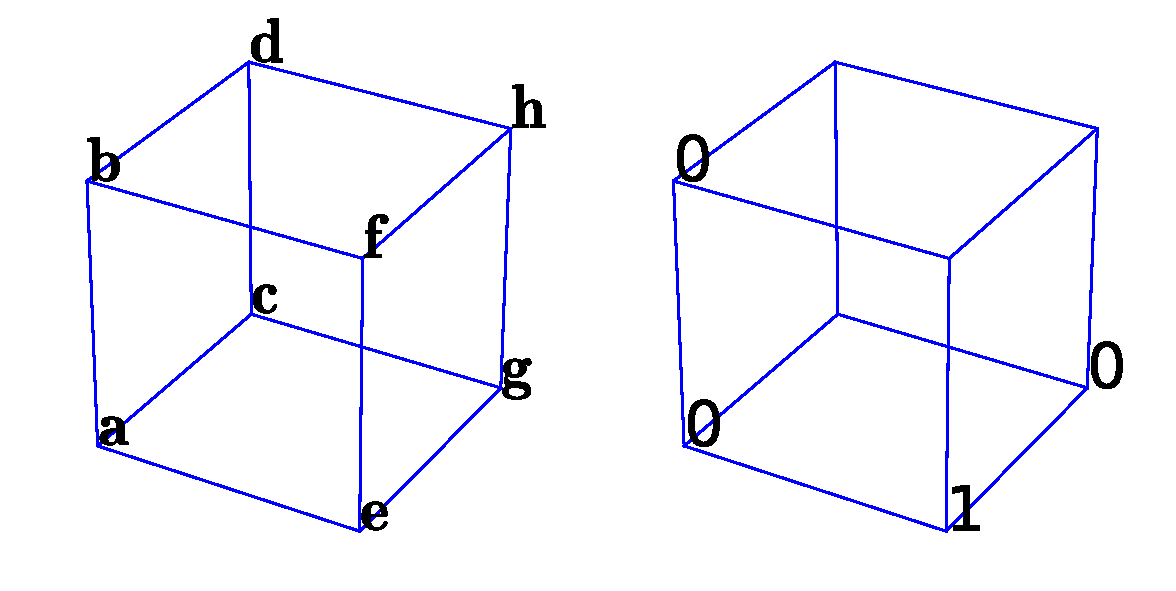
\includegraphics[width=3in]{figures/ae_example.pdf}
  \repeatcaption{FIG:ae_example}{With $S = \Set{\mathbf{a}, \mathbf{b}, \mathbf{d},
  \mathbf{e}}$, we have $\esfs = \Set{\mathbf{c}, \mathbf{f}}$.}
  \label{FIG:ae_example2}
\end{figure}

\begin{table}[t]
  \centering
  $$
  \begin{array}{ccccc}
    \toprule
    \mathbf{b} & \mathbf{d} & \mathbf{a} & \mathbf{g} &  \AD(b_i, d_i, a_i, g_i)\\
    \midrule
    0 & 0 & 0 & 1 &   \textbf{1}\\
    0 & 1 & 0 & 1 &   \textbf{0}\\
    1 & 1 & 0 & 0 &   \textbf{0}\\
    \bottomrule
  \end{array}
  $$
  \caption{$\AD(\mathbf{b}, \mathbf{d}, \mathbf{a}, \mathbf{g}) = 1$.}
  \label{TAB:AD_bdag}
\end{table}



In \cite{BayMicDelIJCAI07}, the authors evaluated this classifier on a Boolean
setting $\mathbb{B}^m$ over 8 benchmarks from the UCI repository.  This
approach led to remarkable results in terms of accuracy, when compared to
off-the-shelf standard classifiers. Nonetheless, this algorithmic description
of the extended classifier does not allow us to grasp its inherent working
behaviour, and it is difficult to extract theoretical properties. The aim of
the next subsection is to give a functional translation of this algorithmic
description.

\subsection{Analogical classifier: a functional definition}
\label{SEC:functional_definition}

As we have previously seen, we can generally assume that
$\AD(\mathbf{a},\mathbf{b},\mathbf{c},\mathbf{d}) \eqdef
\norm{p}{(\mathbf{a}-\mathbf{b})-(\mathbf{c}-\mathbf{d})}$, whether we are
dealing with the arithmetic proportion or the Boolean proportion.
A key observation is that we can formulate this expression with a distance
function on $X^m$. Indeed, a simple rewriting leads to the following expression:
$$\AD(\mathbf{a},\mathbf{b},\mathbf{c},\mathbf{d})=\norm{p}{\mathbf{d} -
(\mathbf{c}-\mathbf{a}+\mathbf{b})}=\norm{p}{\mathbf{d} - \mathbf{d}'},$$
where $\mathbf{d}'\eqdef\mathbf{c}-\mathbf{a}+\mathbf{b}$. Actually,
$\mathbf{d}'$ is nothing but the $4^\text{th}$ vertex of the parallelogram
$\mathbf{a}\mathbf{b}\mathbf{c}\mathbf{d}'$, or equivalently, $\mathbf{d}'$ is
solution of the equation $\mathbf{a}: \mathbf{b} :: \mathbf{c} : \mathbf{x}$.
All this means that $\AD(\mathbf{a},\mathbf{b},\mathbf{c},\mathbf{d})$ simply
is the distance between $\mathbf{d}$ and this $4^\text{th}$ vertex
$\mathbf{d}'$: $\AD(\mathbf{a},\mathbf{b},\mathbf{c},\mathbf{d}) =
\delta_p(\mathbf{d}, \mathbf{d}')$, where $\delta_p$ is the distance defined by
the $p$-norm. Figure \ref{FIG:analogical_dissimilarity} schematically sums up all the aforementioned
properties.  Note that when $(\mathbf{a}, \mathbf{b}, \mathbf{c}) \in S^3$ and
when the associated class equation is solvable, we naturally have $\mathbf{d}'
\in \esf$.
\begin{figure}[!h]
\centering
  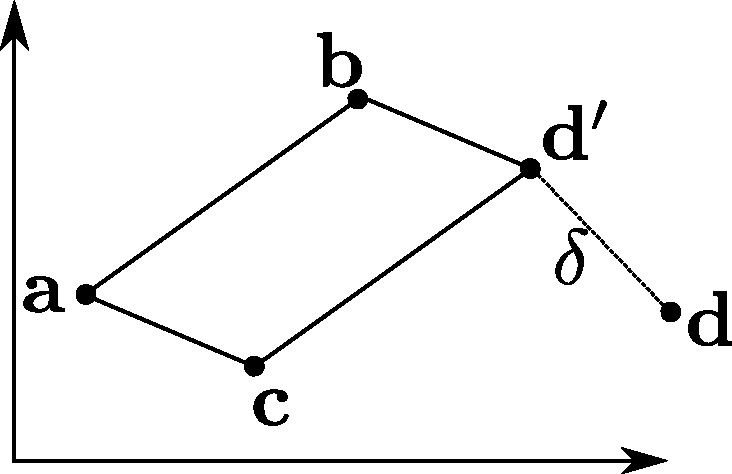
\includegraphics[width=2.5in]{figures/analogical_dissimilarity.pdf}
  \caption{The analogical dissimilarity
  $\AD(\mathbf{a},\mathbf{b},\mathbf{c},\mathbf{d})$ is equal to the distance
  $\delta(\mathbf{d}, \mathbf{d}')$.}
\label{FIG:analogical_dissimilarity}
\end{figure}

\begin{testexample}
Let us consider (again) Figure \ref{FIG:ae_example} on page
\pageref{FIG:ae_example2}. We have already seen that $\AD(\mathbf{b},
\mathbf{d}, \mathbf{a}, \mathbf{g}) = 1$, as proved by Table \ref{TAB:AD_bdag}
  on page \pageref{TAB:AD_bdag}.
We now can reinterpret this statement: $\AD(\mathbf{b}, \mathbf{d}, \mathbf{a},
\mathbf{g})$ should be equal to the distance between $\mathbf{g}$ and another
vector that make up a perfect parallelogram with the $3$-tuple
$(\mathbf{b},\mathbf{d}, \mathbf{a})$. This vector is naturally
$\sol(\mathbf{b},\mathbf{d}, \mathbf{a}) = \mathbf{c}$ and have indeed
$H(\mathbf{c}, \mathbf{g}) =  \AD(\mathbf{b}, \mathbf{d}, \mathbf{a},
\mathbf{g}) = 1$, where $H$ is the hamming distance! The same can be observed
for $\mathbf{h}$: $\AD(\mathbf{a}, \mathbf{b}, \mathbf{e}, \mathbf{h}) =
H(\mathbf{h}, \mathbf{f})$, where $\mathbf{f} = \sol(\mathbf{a}, \mathbf{b},
\mathbf{e})$.
\end{testexample}

We are now finally ready for our unifying functional definition of analogical
classifiers. As we have seen, for a given $\mathbf{x} \in X^m$, Algorithm
\ref{ALGO:extended_classifier} tries to minimize
$\AD(\mathbf{a},\mathbf{b},\mathbf{c},\mathbf{x})$ over all the $3$-tuples
$(\mathbf{a},\mathbf{b},\mathbf{c}) \in S^3$. In the light of what has just
been explained, we see that this is equivalent to finding the closest vertex
$\mathbf{d}' \in \esf$ from $\mathbf{x}$ for any $(\mathbf{a}, \mathbf{b},
\mathbf{c}) \in S^3$. In other words, \textbf{looking for the $k$ $3$-tuples in
$S^3$ that have the smallest value of $\AD$ with $\mathbf{x}$ amounts to
finding the $k$ closest elements to $\mathbf{x}$ in $\esf$}. We will call these
elements the $k$ \textbf{nearest analogical neighbors} of $\mathbf{x}$:

\begin{definition}[The $k$ nearest analogical neighbors]
  \label{DEF:knan}
  For any $\mathbf{x} \in X^m$, and any training set $S \subset X$, we define
  the $k$ nearest analogical neighbors of $\mathbf{x}$ as the set:
  $$k\text{-nan}\left(\mathbf{x}, S\right) \eqdef \Set{\argmin_{\mathbf{d}' \in
  A_E^Y(S)}^k
  \delta(\mathbf{x},\mathbf{d}')},
  $$
  where $\argmin_{\Sigma}^k \delta(\mathbf{x}, \cdot)$ returns the $k$ elements in $\Sigma$
  with the least value of $\delta$.
  Another equivalent way of defining $k\text{-nan}$ is:
  $$k\text{-nan}\left(\mathbf{x}, S\right) \eqdef k\text{-nn}\left(\mathbf{x},
  \esf\right),$$
  where $k\text{-nn}\left(\mathbf{x},\Sigma\right)$ is the set of $k$ nearest
  neighbors of $\mathbf{x}$ in the set $\Sigma$. Ties are broken at random.
\end{definition}

For any $\mathbf{x} \in X^m$, the elements in $\knan(\mathbf{x}, S)$ all belong
to $\esf$, so they all have an analogical label. The prediction
$\hat{f}(\mathbf{x})$ of an extended classifier is thus nothing but the most
frequent analogical label:

\begin{definition}[Extended classifier]
  \label{DEF:extended_classifier}
  Given a training set $S$ with an underlying ground truth function $f$,
  an extended classifier with parameter $k$ sets the prediction of an element
  $\mathbf{x} \in X^m$ as follows:

  $$\hat{f}(\mathbf{x}) \eqdef \text{Mode}\Set{\albl{\mathbf{d}'} | \mathbf{d}'
  \in k\text{-nan}\left(\mathbf{x}, S\right)}.
  $$
\end{definition}

In some sense, an analogical classifier behaves as a $\NN$
classifier\footnote{In the following, $\NN$ and $\NAN$ will denote classifiers.
$\knn$ and $\knan$ denote sets, as in Definition \ref{DEF:knan}.} but
on an extended training set. The above definitions lead us to understand the
process of analogical classification as follows:
\begin{enumerate}
  \item First, extend the training set $S$ to its analogical extension
    $\esf$. $\esf$ can be viewed as an extended training set that has
    \textbf{class noise}: the labels associated with elements in $\esfs$ are
    their analogical labels as defined in Definition
    \ref{DEF:analogical_label}, and they may not be equal to the ground truth
    value $f(\mathbf{x})$.
  \item Then, simply apply a classical $k$-NN strategy over this extended
    training set.
\end{enumerate}

Figure \ref{FIG:extended_classifier} gives an illustration of the classification process for
$k = 1$: the
label of $\mathbf{x} \in X$ is unknown, and we set it to that of $\mathbf{d}'
\in \esf$ (a circle), which is its nearest analogical neighbour. To show that
the analogical label of $\mathbf{d}'$ has itself been inferred, it is depicted
as transparent instead of plain black.
\begin{figure}
\begin{center}
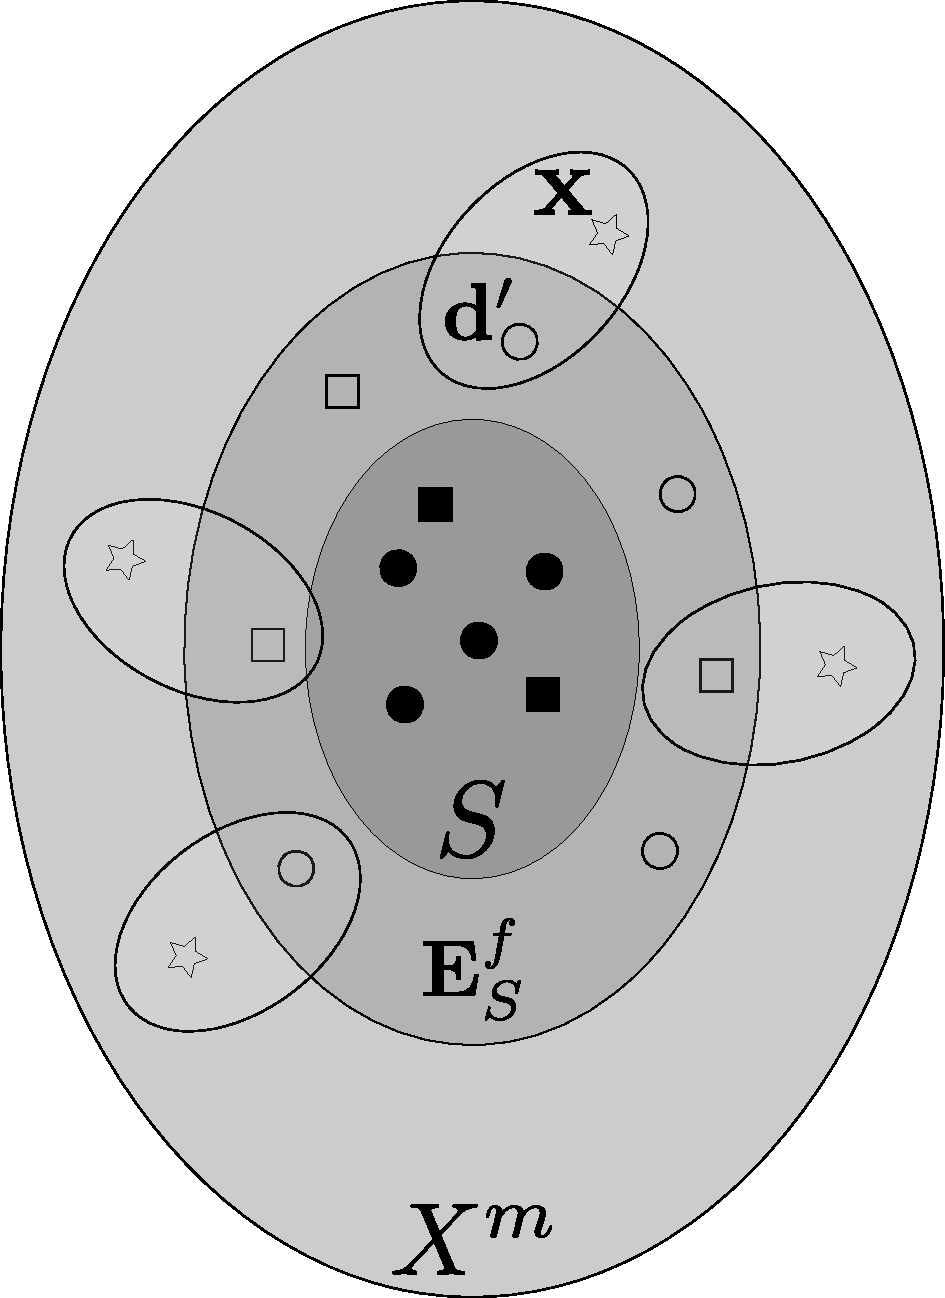
\includegraphics[scale=0.20]{figures/extended_classifier.pdf}
\end{center}
  \caption{Classification process of an extended analogical learner.
  $\hat{f}(\mathbf{x}) = \albl{\mathbf{d}'}$.}
\label{FIG:extended_classifier}
\end{figure}
Let us note that topologically speaking, Figure \ref{FIG:extended_classifier}
is not representative of a real case: even if we always have $S \subseteq \esf
\subseteq X^m$, this does not mean that these sets are embedded into one
another as shown in the drawing. Actually, elements of $S$ (and thus of $\esf$)
are usually scattered over the whole universe.

\begin{testexample}
Going back (for the last time!) to Figure \ref{FIG:ae_example}, our
new functional view allows us to consider the following steps:
\begin{enumerate}
  \item First extend $S = \Set{\mathbf{a}, \mathbf{b}, \mathbf{d}, \mathbf{e}}$
    to $\esf = \Set{\mathbf{a}, \mathbf{b}, \mathbf{c}, \mathbf{d},
    \mathbf{e}}$ with $\hat{f}(\mathbf{c}) = \albl{\mathbf{c}} = 1$ and
    $\hat{f}(\mathbf{f}) = \albl{\mathbf{f}} = 1$.
  \item Then, to classify $\mathbf{g}$, we simply look to its nearest neighbors
    in $\esf$, which are $\mathbf{c}$ and $\mathbf{e}$. The aggregation of
    their analogical labels leads to
    $\hat{f}(\mathbf{g}) = 1$. The nearest neighbors of $\mathbf{h}$ are
    $\mathbf{d}$ and $\mathbf{f}$, which also leads to $\hat{f}(\mathbf{h}) =
    1$.
\end{enumerate}
\end{testexample}

As far as we know, this is the first time a functional definition of
analogy-based classifiers is given. This definition clearly fits with the known
algorithms but obviously, some implementation details cannot be exactly caught
up by such a high level description. It is indeed possible to find a few edge
cases where this functional definition may not output the same result as
algorithm \ref{ALGO:extended_classifier}: this is the case for example when the
nearest analogical neighbor (nan) of $\mathbf{x}$ is not unique. It is also the
case with the Boolean proportion when the closest vertex $\mathbf{d}'$ does not
belong to $\mathbb{B}^m$.  However, as we will see later, these cases are not
likely to occur and the two approaches (that of Algorithm
\ref{ALGO:extended_classifier} and that of Definition
\ref{DEF:extended_classifier}) produce very similar results, thus empirically
validating this functional definition.

Since we now have a clear functional definition of analogical classifiers, we
are in position to examine some general theoretical properties of analogical
learners. This is the purpose of the next section.
\section{Theoretical properties of analogical classifiers}
\label{SEC:theoretical_properties_of_analogical_classifiers}

The functional definition of analogical learners opens the door the study of
various theoretical properties of analogical classifiers, which had only been
described algorithmically so far. Just like for the $k$-NN literature,
theoretical results are easier to derive when $k = 1$. We will therefore mostly
focus on the properties of the 1-NAN classifier.
\subsection{Study of convergence}

Let us consider the case where $X^m=\mathbb{R}^m$, and let $\delta$ be any
distance function defined from a norm. Simply because $S \subseteq \esf$ for
any $S$, the
following inequality holds for any $\mathbf{x} \in X^m$ :
$$\delta(\mathbf{x}, \nan(\mathbf{x},S)) \leq \delta(\mathbf{x},
\nn(\mathbf{x},S)).$$


Now, let us consider  $\mathbf{x}^{(i)}$ an i.i.d. sequence of random variables
in $\mathbb{R}^m$, where $\mathbb{R}^m$ is equipped with a probability measure
denoted $P$. The training set will be denoted $S_n=\Set{\mathbf{x}^{(i)}, ~ i
\in [1, n]}$. As $S_n$ is random, then $\nan(\mathbf{x},S_n)$ can also be
considered as a random element of $X^m$.  We then are in the exactly same
context as the work of Cover \& Hart (\cite{CovHarTIT67}), and we obtain the
same result:
\begin{property}
  \label{PROPER:convergence_nan}
  For any $\mathbf{x}$, its nan $\nanemph(\mathbf{x}, S_n)$ converges almost
  surely towards $\mathbf{x}$ as $n$ tends to infinity:
  $$P\left(\lim_{n \to \infty} \nanemph(\mathbf{x}, S_n) = \mathbf{x}\right) =
  1.$$
\end{property}
\begin{proof}
  The proof can be easily derived from the results of Cover \& Hart in
  \cite{CovHarTIT67}. Indeed, they have already showed that the nearest neighbor of
  $\mathbf{x}$ converges almost surely towards $\mathbf{x}$ as $n$ tends to
  infinity:
  $$P\left(\lim_{n \to \infty} \nn(\mathbf{x}, S_n) = \mathbf{x}\right) =
  1.$$
  To prove this result, they simply start from the fact that
  $\delta(\mathbf{x}, \nn(\mathbf{x}, S_n))$ converges in probability towards
  $0$:
  $$\forall \epsilon > 0,~~P\Big(\delta(\mathbf{x}, \nn(\mathbf{x}, S_n)) >
  \epsilon\Big) = 0.$$
  Using the previous fact that $\delta(\mathbf{x}, \nan(\mathbf{x},S_n)) \leq
  \delta(\mathbf{x}, \nn(\mathbf{x},S_n))$, the convergence in probability of
  $\delta(\mathbf{x}, \nan(\mathbf{x},S_n))$ towards $0$ is immediate. Then, it
  naturally follows that $\nan(\mathbf{x}, S_n)$ converges almost surely
  towards $\mathbf{x}$, following the same steps as Cover \& Hart.
\end{proof}

Let us note the following points:
\begin{enumerate}
\item The result of Cover and Hart was actually proved in a less restrictive
  setting than ours. They have proven their result for any separable metric
    space, without any additional structure. Unfortunately, we are not able to
    follow these lines here, because there is no known way to define an
    analogical dissimilarity on a metric space, without the help of any other
    structure or operator (see \cite{MicBayDelJAIR08} for a detailed discussion
    on this issue).
  \item Cover \& Hart proved that when $n$ tends to infinity, the probability
    of error of the $1$-\NN classifier is less than twice that of the Bayes
    probability of error, and therefore less than twice the probability of error of
    any other classifier. We have not been able to prove such a strong result
    for the $1$-\NAN~classifier, but its probability of error will be thoroughly
    investigated in Subsection \ref{SEC:accuracy_analysis}.
  \item We have to be careful about the interpretation of Property
    \ref{PROPER:convergence_nan} in terms of machine learning. Indeed, another
    key property is proved in \cite{CovHarTIT67}: for an integrable
    function $f$  over $\mathbb{R}^m$ w.r.t. the probability measure $P$, the
    expectation of $f(\nn(\mathbf{x},S_n))- f(\mathbf{x})$ converges to 0 when
    $n$ tends to infinity.  This means that asymptotically, the nearest
    neighbour of $\mathbf{x}$ has the same properties as $\mathbf{x}$, and
    particularly: \textbf{they have the same label}, which is a very powerful
    property when we are dealing with a classification task. Sadly, such a
    property has not been proven for $\nan(\mathbf{x}, S_n)$.
\item Finally, it is clear that when $n$ goes to infinity, the behavior of an
  analogical classifier tends to that of a nearest neighbours classifier.
    Indeed, when $S_n$ is very big, the nearest analogical neighbour of an
    element $\mathbf{x}$ simply is its nearest neighbour, in most cases.
    Moreover, when the nan and the nn are too close, paying the price of the
    noise related to the nan may not be worth it. This supports the common
    acknowledgement that analogical reasoning is mostly useful when very few
    data are available.  In this later case extending a small training set with
    its analogical extension may be particularly beneficial, as we will see in
    Chapter \ref{CHAP:analogy_preserving_functions}.

\end{enumerate}
To conclude this discussion, even if the convergence result is interesting in
itself, it does not say a lot in terms of machine learning. A much more
interesting and powerful theoretical result of analogical classifiers will be
proved in Chapter \ref{CHAP:analogy_preserving_functions}.

\subsection{Vapnik Chervonenkis (VC) dimension}
\label{SEC:VCdim}
The notion of VC-dimension was originally defined by Vapnik and Chervonenkis
\cite{Vap98}, and introduced into learnability theory by Blumer et al.
\cite{BluEhrHauWarACM89}. Roughly speaking, the VC-dimension (denoted VC) of a class of
learners is a numerical measure of their discrimination power. One of the main
results about the VC-dimension is that it allows to bound the true risk $R$ of
a learner. With probability $1 - \eta$, and under some theoretical conditions
that we omit here, we have:

$$R \leq R_{\text{emp}} + \sqrt{\frac{1}{n} \cdot \left[\text{VC}(\log(2n /
\text{VC}) + 1) - \log(\eta/4)\right]},$$
where $R_\text{emp}$ is the probability of error on a training set $S$ of size
$n$, and VC is the VC-dimension of the learner. In our setting,
\begin{itemize}
  \item $R \eqdef P\left(\hat{f}(\mathbf{x}) \neq f(\mathbf{x}) \given[\big]
    \mathbf{x} \in X^m\right)$, and
  \item $R_\text{emp} \eqdef P\left(\hat{f}(\mathbf{x}) \neq f(\mathbf{x})
    \given[\big] \mathbf{x} \in S_n\right)$.
\end{itemize}

This theoretical upper bound on the true risk $R$ is what makes the
VC-dimension of a class of learners an essential element of their theoretical
study. The VC-dimension is defined as follows:

\begin{definition}[VC-dimension]
  \label{DEF:VCdim}
  We consider a class of learners $\mathcal{C}$ and a set $S_n$ of $n$ labeled
  elements in $X^m$. There are exactly $2^n$ ways to label each of the $n$
  elements. If for any labeling, there exist a learner in $\mathcal{C}$ that
  correctly labels all the elements in $S_n$, we say that $\mathcal{C}$
  \textbf{shatters} $S_n$.\\

  The VC-dimension of $\mathcal{C}$ is the biggest $n$ such that there exist a
  set of $n$ points $S_n$ that can be shattered by $\mathcal{C}$.
\end{definition}

%We consider a universe $X$ (usually a Cartesian product to represent the data)
%and a family $\mathcal{H}=\{h_i \subseteq X|i \in I\}$ of subsets of $X$.  The
%elements of $\mathcal{H}$ will be referred as hypothesis or models.  Given a
%subset $A$ of $X$, we can consider the new family of subsets $tr(\mathcal{H},A)
%= \{h_i \cap A \subseteq X|i \in I\}$: this family is called the {\it trace of
%$\mathcal{H}$ over $A$}. This is obviously a subset of the power set of $A$,
%$2^A$ i.e. $tr(\mathcal{H},A) \subseteq 2^A$.  We say that $\mathcal{H}$
%shatters $A$ iff $tr(\mathcal{H},A)=2^A$.  $VC\mbox{-}dim(\mathcal{H})$ is then
%the size of the largest finite subset which can be shattered by $\mathcal{H}$:
%\begin{definition} $VC\mbox{-}dim(\mathcal{H}) = \bigsqcup \{|A| \given[\big]
%  \mathcal{H} \mbox{ shatters } A \}$,
%\end{definition}
%where $\bigsqcup$ is the least upper bound operator.  In the case where
%$\forall n \in\mathbb{N}, \exists  A \subset X, |A|=n \mbox{ such that }
%\mathcal{H} \mbox{ shatters } A$, we simply say that:
%$$VC\mbox{-}dim(\mathcal{H})=\infty.$$ \noindent
%As a binary classifier $c$ over $X$ defines a subset of $X$ with $c^{-1}(1)=\{x
%\in X | c(x)=1\}$, we can associate to a class $\mathcal{C}$ of classifiers a
%family of subsets $\{c^{-1}(1) | c \in \mathcal{C}\}$ and then the
%$VC\mbox{-}$dimension of a set of classifiers is as below:
%\begin{definition}
%$VC\mbox{-}dim(\mathcal{C})=VC\mbox{-}dim(\{c^{-1}(1) | c \in \mathcal{C}\})$
%\end{definition}

Let's first consider the class of nearest neighbors classifiers:
$\mathcal{C}_{\text{NN}}=\{ k\text{-NN classifiers}, k \in \mathbb{N}^*\}$. It
is clear that the VC-dimension of $\mathcal{C}_{\text{NN}}$ is infinite: taking
$k = 1$, any training set of any size can be perfectly labeled by 1-NN,
because every element is its own nearest neighbor. Actually, we can easily show
the same result for the analogical learners.

\begin{proposition}
  \label{PROPOS:VCdim}
  The class $\mathcal{AC}_k$ of analogical learners has infinite VC-dimension.
\end{proposition}
\begin{proof}
  Considering Definition \ref{DEF:extended_classifier} on page
  \pageref{DEF:extended_classifier} with $k = 1$, we see
  that the predicted label of any element $\mathbf{x}$ is that of its nan. For
  any element $\mathbf{x}$ in $S_n$, $\mathbf{x}$ is its own nan (just like
  $\mathbf{x}$ is its own nearest neighbor). Hence, any training set $S_n$ of
  size $n$ is correctly labeled by 1-NAN, and thus can be shattered by
  $\mathcal{AC}_k$. Therefore, the VC-dimension of $\mathcal{AC}_k$ is infinite.
\end{proof}

Clearly, the upper bound is a decreasing function in $n$, and an increasing
function in the VC dimension of the learner. As such, we usually want the
VC-dimension of our classifiers to be small. However, we have previously seen
that the nearest neighbors classifiers, despite their infinite
VC-dimension, enjoy many interesting theoretical properties, and their
practical efficiency is well-acknowledged. In fact, the upper bound on the true
risk does not even hold for classes of learner whose VC-dimension is infinite
\cite{Bur98}. We then need to keep in mind that even though the analogical
learners have an infinite VC-dimension, which is an interesting result in its
own right, this does not necessarily prevent them from being useful
classifiers.

\subsection{Accuracy analysis}
\label{SEC:accuracy_analysis}

In this section, we study the accuracy of an analogical classifier, and more
particularly that of the $\NAN$ classifier. As explained in Section
\ref{SEC:functional_definition}, for a given $\mathbf{x} \in X^m$ and a
training set $S \subset X^m$, the prediction $\hat{f}(\mathbf{x})$ is set as:
$$
\hat{f}(\mathbf{x}) ~ \eqdef ~ \albl{\nan(\mathbf{x}, S)} ~ \eqdef ~ \albl{\nn(\mathbf{x}, \esf)}.
$$

We now equip the set $X^m$ with a probability distribution denoted $P$.  The
accuracy of the $\NAN_S$ classifier\footnote{The $S$ subscript is here to
specify that the training set of the $\NAN$ algorithm is $S$. The same notation
is used for the \textit{nearest neighbour} algorithm: $\NN_\Sigma$ is the $\NN$
algorithm trained on the set $\Sigma$.} over all the elements of $X^m$ is
defined as:
$$\acc(\NAN_S, X^m)\eqdef P\left(\hat{f}(\mathbf{x})=f(\mathbf{x}) \given[\big]
\mathbf{x} \in X^m\right).$$
Our main result is given by Proposition \ref{PROPOS:accuracy_nan}:
\begin{proposition}
  \label{PROPOS:accuracy_nan}
  The accuracy of $\NAN_S$ over $X^m$ can be seen as the weighted sum of the
  accuracy of $\NN$ over $A$ and $B$, using a different training set each time
  (respectively $S$ and $\esfs$):
  \begin{align*}
    \acc(\NAN_S, X^m) = ~&\acc(\NN_S, A) \cdot \alpha ~ + \\
                        &\acc(\NN_{\esfs}, B) \cdot (1 - \alpha),
  \end{align*}
  where:
  \begin{itemize}
  \item $A \eqdef \set{\mathbf{x} \in X^m | \nan(\mathbf{x}, S) \in S}$: the
    elements that have their nan in $S$.
  \item $B \eqdef \set{\mathbf{x} \in X^m | \nan(\mathbf{x}, S) \in \esfs}$: the
    elements that have their nan in $\esfs$.
  \item $\alpha \eqdef P(\mathbf{x} \in A)$ and $1 - \alpha = P(\mathbf{x} \in
    B)$. 
  \end{itemize}
  Naturally, $A \cup B = X^m$ and $A \cap B = \varnothing$.
\end{proposition}
\begin{proof}
By observing that for any $\mathbf{x}$, its $\nan$ either belongs to $S$ or to
$\esfs$, the accuracy $\acc(\NAN_S, X^m)$ can be split into two distinct parts as follows:

\begin{align*}
  &\acc(\NAN_S, X^m) \eqdef P\left(\hat{f}(\mathbf{x})=f(\mathbf{x}) \given[\big] \mathbf{x} \in
  X^m\right) = P\left(\albl{\nan(\mathbf{x}, S)} = f(\mathbf{x})\right)\\
  =~&P\left([\albl{\nan(\mathbf{x}, S)} = f(\mathbf{x}) ]\wedge
  [\nan(\mathbf{x}, S) \in S ] \right)~ +
  P\left([\albl{\nan(\mathbf{x}, S)} = f(\mathbf{x})] \wedge [\nan(\mathbf{x},
  S) \in \esfs]\right)\\
  =~&P\left([\albl{\nn(\mathbf{x}, \esf)} = f(\mathbf{x})] \wedge
  [\nn(\mathbf{x}, \esf) \in S ]\right)~ +
  P\left([\albl{\nn(\mathbf{x}, \esf)} = f(\mathbf{x})] \wedge
  [\nn(\mathbf{x}, \esf) \in \esfs]\right) \\
  =~&P\left([\albl{\nn(\mathbf{x}, \esf)} = f(\mathbf{x})] \given[\big]
  [\nn(\mathbf{x}, \esf) \in S ]\right) \times
  P\left([\nn(\mathbf{x}, \esf) \in S]\right) ~+ \\
  &P\left([\albl{\nn(\mathbf{x}, \esf)} = f(\mathbf{x})] \given[\big]
  [\nn(\mathbf{x}, \esf) \in \esfs]\right) \times
  P\left([ \nn(\mathbf{x}, \esf) \in \esfs]\right)
\end{align*}

Let us denote  $\alpha \eqdef P\left(\nn(\mathbf{x}, \esf) \in S\right)$.
Obviously, we also have $\alpha \eqdef P\left(\nan(\mathbf{x}, S) \in
S\right)$.  The above formula becomes:
\begin{align*}
  &\acc(\NAN_S, X^m) = \\&P\left([\albl{\nn(\mathbf{x}, \esf)} = f(\mathbf{x})]
  \given[\big] [\nn(\mathbf{x}, \esf) \in S] \right) * \alpha ~+ \\
  &P\left([\albl{\nn(\mathbf{x}, \esf)} = f(\mathbf{x})] \given[\big]
  [\nn(\mathbf{x}, \esf) \in \esfs]\right) * (1 - \alpha).
\end{align*}

Let us focus on the first term, temporarily discarding the factor $\alpha$:
$$P\left([\albl{\nn(\mathbf{x}, \esf)} = f(\mathbf{x})] \given[\big]
[\nn(\mathbf{x}, \esf) \in S] \right).$$

It is easy to see that the event $[\nn(\mathbf{x}, \esf) \in S]$ is equivalent
to the event $[\nn(\mathbf{x}, \esf) = \nn(\mathbf{x}, S)]$. As a result, we
can transform the first term to get a better grasp of its meaning:
\begin{align*}
  &P\left([\albl{\nn(\mathbf{x}, \esf)} = f(\mathbf{x})] \given[\big]
  [\nn(\mathbf{x}, \esf) \in S] \right)\\
  =~ &P\left([\albl{\nn(\mathbf{x},\esf)} = f(\mathbf{x})] \given[\big]
  [\nn(\mathbf{x}, \esf) = \nn(\mathbf{x}, S)]\right)\\
  =~ &P\left([\albl{\nn(\mathbf{x}, S)} = f(\mathbf{x})] \given[\big]
  [\nn(\mathbf{x}, \esf) \in S]\right).
\end{align*}

In this form, the first term is just the accuracy of the $\NN_S$ algorithm over
the elements that have their nearest analogical neighbour in $S$.
As for the second term, the same process can be applied by observing that the
event $[\nn(\mathbf{x}, \esf) \in\esfs]$ is equivalent to the event
$[\nn(\mathbf{x}, \esf) = \nn(\mathbf{x}, \esfs)]$. This leads to
\begin{align*}
  &P\left([\albl{\nn(\mathbf{x}, \esf)} = f(\mathbf{x})] \given[\big]
  [\nn(\mathbf{x}, \esf) \in \esfs]\right)\\
  =~ &P\left([\albl{\nn(\mathbf{x}, \esfs)} = f(\mathbf{x})] \given[\big]
  [\nn(\mathbf{x}, \esf) \in \esfs]\right).
\end{align*}

This second term is then the accuracy of the $\NN_{\esfs}$ algorithm over the
elements that have their nearest analogical neighbour in $\esfs$.

In the light of these interpretations, we can directly rewrite the accuracy
formula in a the concise form given in Proposition \ref{PROPOS:accuracy_nan}.
\end{proof}

The value $\acc(\NN_S, A)$ is the accuracy of $\NN_S$ over all the elements in
$A$. A theoretical study of this accuracy has been done in \cite{LanIbaIJCAI93}
when the size of $A$ is known.  Regarding $\acc(\NN_{\esfs}, B)$, this is the
accuracy of $1$-$\NN$ when the training set is
noisy, and has been studied in \cite{OkaYugIJCAI97}. This last formula leads
to the consistent facts:
\begin{enumerate}
\item The smaller $\esfs$ (i.e. analogical reasoning does not
  bring much more labels), the closer $\alpha$ is to $1$, the closer $A$ is to
  $X^m$ and the more the accuracy of $\NAN_S$ tends towards the accuracy of
  $\NN_S$ over $X^m$.
\item In return, if $\esf$ is much bigger than $S$, $\alpha$ is then small, $B$
  is close to $X^m$ and the accuracy of $\NAN_S$ greatly depends on the quality
  of $\esf$:  \end{enumerate}

\begin{definition}[Quality of the analogical extension $\omegasf$]
  \label{DEF:omega}
  Given a training set $S\subset X^m$ and a ground truth function $f$, the
  \textbf{quality} of the analogical extension $\esf$ is defined as:
  $$
  \omegasf \eqdef P\left(\albl{\mathbf{x}} = f(\mathbf{x}) \given[\big]
  \mathbf{x} \in \esfs\right).$$
  Note that the value $1 - \omegasf$ corresponds to the class noise of $\esfs$.
\end{definition}

This closes our contributions to the theoretical properties of analogical
classifiers. In the next section, we empirically investigate and illustrate the
soundness of our results.

\section{Experiments and empirical validation}
\label{SEC:experiments_and_empirical_validation}
In order to get an empirical validation of our formulas, we have developed a
set of experiments that we now describe.

\subsection{Evaluation protocol}

Working with Boolean vectors, we have computed the accuracies of the 1-\NAN~and
1-$\NN$~ algorithms over $X=\mathbb{B}^m$ for $m = 8$. Other values of $m$ have
been investigated, leading to very similar results.  The ground truth label of
the elements of $X^m$ is defined by different Boolean functions $f$:
\begin{itemize}
\item $f_1(\mathbf{x})=x_i$ for some $i$. These functions are called
  projections, or dictators.  They lead to perfectly linearly
    separable problems, i.e.  there exist an hyperplane that can perfectly
    discriminate both classes. As such, they are expected to be fairly easy to
    learn.
  \item $f_2(\mathbf{x})= \bigoplus_{i = 1}^k  x_i$ for some $k \in[1, m]$, where $\oplus$
    is the XOR operator (which is associative). These functions
    lead to highly non-linearly-separable problems: remember the example of
    Figure \ref{FIG:classification_problem} on page
    \pageref{FIG:classification_problem}, who was an instance of a XOR problem.
    XOR problems are traditionally difficult to learn.
  \item $f_3(\mathbf{x})= \bigwedge_{i = 1}^k  x_i$ for some $k \in [1, m]$.
  \item $f_4(\mathbf{x})= \bigvee_{i = 1}^k  x_i$ for some $k\in [1, m]$.
  \item $f_5(\mathbf{x}) = \left[\sum_{i = 1}^m x_i \geq k\right]$ for some $k
    \in [1, m]$, where the function $[\text{cond}]$ is equal to $1$ if cond is
    verified and $0$ else. Simply put, $f(\mathbf{x}) = 1$ iff at least $k$
    components are equal to $1$.
  \item $f_6(\mathbf{x}) = \left[\sum_{i = 1}^m x_i = k\right]$ for some $k
    \in [1, m]$. Simply put, $f(\mathbf{x}) = 1$ iff exactly $k$ components
    are equal to $1$.
\end{itemize}


Regarding the size of the training set, to be sure to fit with the size of the
universe, we have investigated various sizes between $3$ and $100$. When
dealing with a training set of size $100$, the cubic complexity of the
analogical classifier leads to explore a set of approximately $100^3$ elements:
as a consequence, we limit our investigation to a maximum of 100 elements in
the training set in order to get realistic execution time.

All the accuracy (and other metrics) computations are averaged over a set of
100 experiments. We have made sure that the class distributions of the training
sets are as close as possible to that of the whole universe $X^m$.  Note that
our implementation of the $\NAN$ algorithm is not that of algorithm
\ref{ALGO:extended_classifier}, but is instead that of the functional
definition of the analogical classifier as described in Definition
\ref{DEF:extended_classifier}: we first construct the analogical extension set
of $S$, and then proceed to a nearest neighbour strategy over this noisy
extended training set. We have estimated probabilities by frequencies, thus
implicitly assuming a uniform distribution on $X^m$.

For each experiment, we have computed the following measures to empirically
investigate the behaviour of the analogical classifier, and assess our
theoretical results:
\begin{itemize}
  \item The empirical accuracy of the 1NAN classifier, defined\footnote{We
    notice here that $\mathbf{x}$ is only required to belong to $X^m \setminus
    S$ and not to $X^m$, because classifying elements in $S$ is pointless.}
    as\\
    $\acc(\NAN_S) \eqdef P\left(\hat{f}(\mathbf{x}) = f(\mathbf{x})
    \given[\big] \mathbf{x} \in X^m \setminus S \right)$.
  \item The empirical accuracy of the 1NN classifier, which definition is of
    course the same but this time $\hat{f}$ is the output of the 1NN
    classifier.
  \item The \textbf{theoretical} accuracy of 1NAN, as defined in Proposition
    \ref{PROPOS:accuracy_nan}. The probability $\alpha \eqdef P(\mathbf{x} \in
    A$) has been estimated by the frequency $\frac{\mid A \mid}{\mid X^m
    \mid}$. Both sets $A$ and $B$ are easy to determine.
  \item The quality of $\esf$, measured by $\omegasf$ as previously defined in
    Definition  \ref{DEF:omega}. $\omegasf$ has been estimated by the
    frequency $\frac{\big| \Set{\mathbf{x} \in \esfs | \albl{\mathbf{x}} =
    f(\mathbf{x}}\big|}{\big| \esfs \big|}$.
  \item Finally, the quantity $\gamma_S^f \eqdef P(\mathbf{x} \in \esf)$,
    estimated by $\frac{\mid \esf\mid}{\mid X^m \mid}$: the size of the
    analogical extension with respect to that of the whole universe.
\end{itemize}

It is fairly easy to see that both functions $f_1$ and $f_2$ split the universe $X^m$ into
two disjoint sets of size $2^{m - 1}$: those for which $f(\mathbf{x})$ is
equal to $1$, and those with labels equal to $0$. We say that the datasets are
balanced. However, the other functions may lead to very unbalanced datasets. An
extreme case is for example $f_3$ with $k = m$, which leads to $f_3(\mathbf{x})
= x_1 \wedge x_2 \wedge \cdots \wedge x_m$. The only element whose label is $1$
is the vector $\mathbf{x} = (1, 1, \cdots, 1)$. For these very unbalanced
datasets, the accuracy of a classifier is not a relevant measure: predicting
$0$ all the time would lead to an accuracy of almost $1$, but would
systematically assign the wrong label to   $(1, 1, \cdots 1)$. Therefore, as
accuracy is our main concern here, we will focus on functions for which
datasets are as balanced as possible.

In addition to these Boolean functions, we have also run the $\NAN$ algorithm
over the Monk datasets over the UCI
repository\footnote{\url{https://archive.ics.uci.edu/ml/datasets/MONK's+Problems}}.
They are datasets of 432 binarized elements, among which exactly 169 of them
have been used for training.

\subsection{Comments and discussion}

Our experiments are summed-up by Figure \ref{FIG:nan_vs_nn} on page
\pageref{FIG:nan_vs_nn}. As they are the result of multiple averaged
experiments, the measures $\omegasf$ and $\gamma_S^f$ are here denoted $\omega$
and $\gamma$. Paying careful attention to these plots will allow us to draw
interesting conclusions about the behaviour of the 1-NAN algorithm.

\begin{figure}[!h]
\centering
  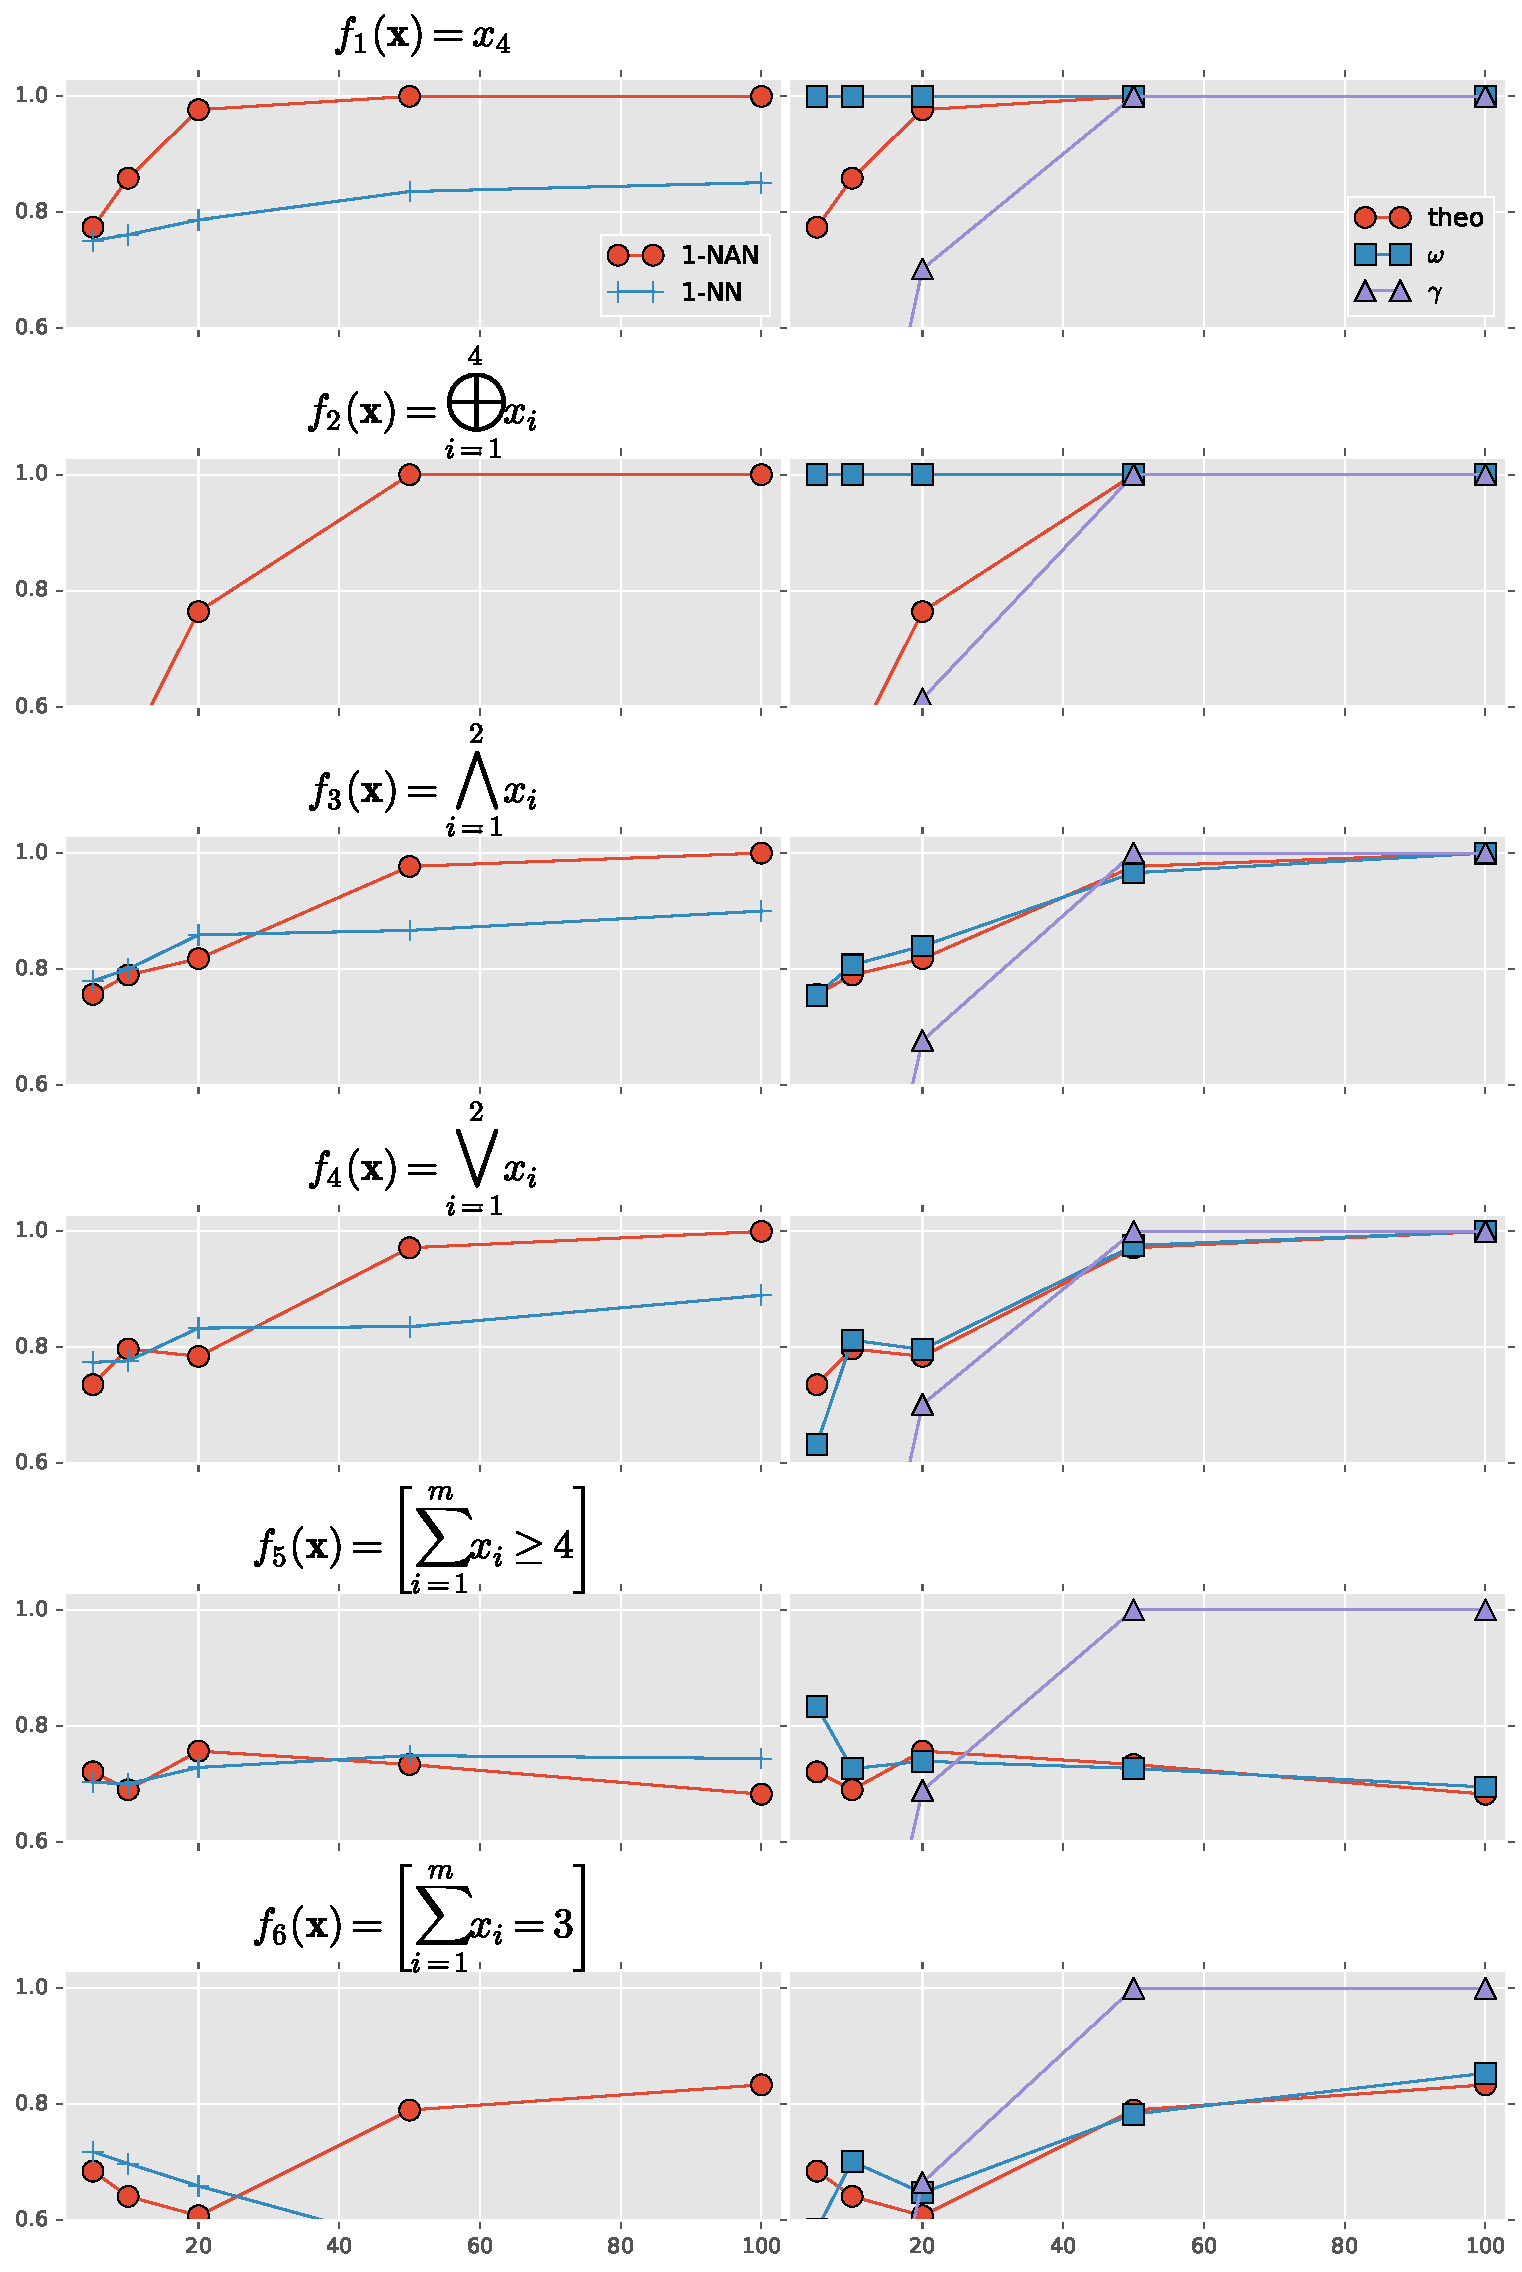
\includegraphics[scale=.50]{figures/nan_vs_nn_SUMMARY_dim8_nexp15.pdf}
  \caption{Accuracies (left) of the 1-NAN and 1-NN algorithms over different
  Boolean functions ($m = 8$) and training set sizes, with corresponding values
  of $\omega$, $\gamma$, and theoretical accuracy (right). The $x$ axis
  corresponds to the size of the training set.}
\label{FIG:nan_vs_nn}
\end{figure}

First, the theoretical accuracy seems to fit perfectly with the empirical
accuracy of the $\NAN$ algorithm, thus validating our theoretical study that
led to proposition \ref{PROPOS:accuracy_nan}. Actually, the maximal difference
we observed between the theoretical accuracy and its actual value is of about
$10^{-10}$.

An interesting observation is that the value of $\omega$ seems to always
converge to that of the theoretical accuracy (and therefore to the actual
accuracy) of $\NAN$. This can be easily explained by paying attention to the
value of $\gamma$, the proportion of elements of $X^m$ that belong to $\esf$.
We see that in any setting, $\gamma$ converges to 1 as $\mid S \mid$ grows.
This means that when $\mid S \mid$ is big enough (but not necessarily
\textit{that} big with respect to $X^m$), the analogical extension of $S$
covers the whole universe $X^m$ (obviously, the bigger the dimension $m$, the
slower the convergence occurs): every element $\mathbf{x}$ is then its own
nearest analogical neighbour and $\hat{f}(\mathbf{x}) = \albl{\mathbf{x}}$. It
is therefore straightforward to see that in this case,
$$
  \omega \eqdef P\left(\albl{\mathbf{x}} = f(\mathbf{x}) \given[\big]
  \mathbf{x} \in \esfs\right) = P\left(\hat{f}(\mathbf{x}) = f(\mathbf{x})
  \given[\big] \mathbf{x} \in \esfs\right)\\ = \acc(\NAN_S, \esfs).
$$
When $\gamma = 1$, the only elements $\mathbf{x}$ we want to classify belong to
$\esfs$ (otherwise they would be in $S$), so this last term exactly corresponds
to the accuracy of the classifier. Another way to see it is to observe that the
first term of the expression of Proposition (\ref{PROPOS:accuracy_nan})
$\acc(\NN_{S}, A) \cdot \alpha$ is zero
because $\alpha = 0$. Only the second term $\acc(\NN_{\esfs}, B) \cdot (1 -
\alpha)$ is of importance, and its value corresponds to $\omega$. As expected,
this observation allows us to state that estimating the value of $\omega$ is
paramount to have a precise idea of the accuracy of an analogical classifier.
%We will provide in the next subsection a method to accurately estimate this
%quantity $\omega$ with the only help of the training set $S$.

A striking result of the experiments is that for the two functions
$f_1(\mathbf{x}) = x_4$ and $f_2(\mathbf{x}) = x_1 \oplus \cdots \oplus x_4$,
the analogical labels are always correctly predicted: $\omega = 1$, i.e. there
is no class noise. However, the accuracy of 1-NAN is not necessarily equal to
$1$ especially for $f_2$ with small training set sizes. The reason is simple:
even if all the elements in $\esf$ are correctly classified, $\esf$ does not
cover the whole space ($\gamma < 1$) so the accuracy of 1-NAN still depends on
that of 1-NN. While the accuracy of 1-NN over $f_1$ is not too bad, the one
over $f_2$ is absolutely terrible and actually below $0.3$ (a random prediction
would have done better!). This is one of the distinguishing features of the XOR
functions: the nearest neighbor of an element is almost always in a different
class, as can be seen on Figure \ref{FIG:classification_problem} (page
\ref{FIG:classification_problem}). So sadly, the 1-NN algorithm can do nothing
but wrong on these kind of functions. In Chapter
\ref{CHAP:analogy_preserving_functions}, we will prove a strong result showing
that both the projections (like $f_1$) and the XOR functions (like $f_2$)
\textbf{always} lead to perfectly sound extensions, for any training set of any
size.

Table \ref{TAB:monks} shows the same metrics for the Monk datasets and also
reports the results of the Analogical Proportion Classifier (\textit{APC}) from
\cite{MicBayDelJAIR08}, which corresponds to algorithm
\ref{ALGO:extended_classifier} with $k=100$.
\begin{table}
\centering
\begin{tabular}{ l  c  c c  c  c }
\toprule
& 1-NAN  & APC & 1-NN  &  $\omegasf$ & $\gamma_S^f$ \\
\midrule
Monk 1 & .961 & .98 & .787 &   .961    &   1 \\
Monk 2 & .998 & 1 & .738 &    .998    &   1 \\
Monk 3 & .963 & .96 & .829 &   .963    &   1 \\
\bottomrule
\end{tabular}
\caption{Accuracies of the 1-NAN, APC and 1-NN algorithms over the Monk
  datasets.}
  \label{TAB:monks}
\end{table}
We note that the functional $\NAN$ approach (almost) achieves the same results
as the somewhat more complex algorithm described in Section
\ref{SEC:extended_classifier}, and that here again the analogical extension set
covers the whole universe: this means that a conservative approach would have
been sufficient! Actually, this raises the following question: why would we
want to look for more than one analogical neighbour when every element of the
universe is already in $\esf$, and therefore \textit{analogically linked} to
those in $S$? Our experiments tend to show that this becomes superfluous,
provided that the training set is big enough.

%\subsection{Estimation of the prediction accuracy}
%
%We have seen in the previous subsection that the value $\omega$ is that of the actual
%accuracy of an analogical classifier when $S$ is big enough. This leads to the
%following question: how can we get a precise estimation of this value $\omega$
%? Answering this would allow us to have a very precise idea of the accuracy we
%can expect from our classifier.
%
%The method we propose for estimating $\omega$ only relies on the training set $S$
%and is very simple: it consists of applying the conservative algorithm to all
%the elements of $S$, and compute the fraction of these elements that have been
%correctly classified. A small yet important modification to the algorithm needs
%to be added: we only want to construct analogical proportions of the form $a :
%b :: c : x$ where $a$, $b$, $c$ and $x$ are all distinct elements. Indeed, the
%proportions $x : x :: x : x$ and $x' : x :: x' : x$ are always true, and the
%solution label related to these proportions would bias the final majority vote
%procedure in a significant way towards the real label $\dot{x}$.
%
%We have applied this estimation protocol to all of the Boolean settings we have
%considered, and it has shown to be very accurate. Figure \ref{omegaplots}
%illustrates a few of these settings (already considered in Figure \ref{plots}).
%\begin{figure}
%  \caption{Values of $\omega$ and its estimation $\hat{\omega}$ for $f_1$, $f_2$ and $f_3$ in
%  $\mathbb{B}^{10}$.}
%\label{omegaplots}
%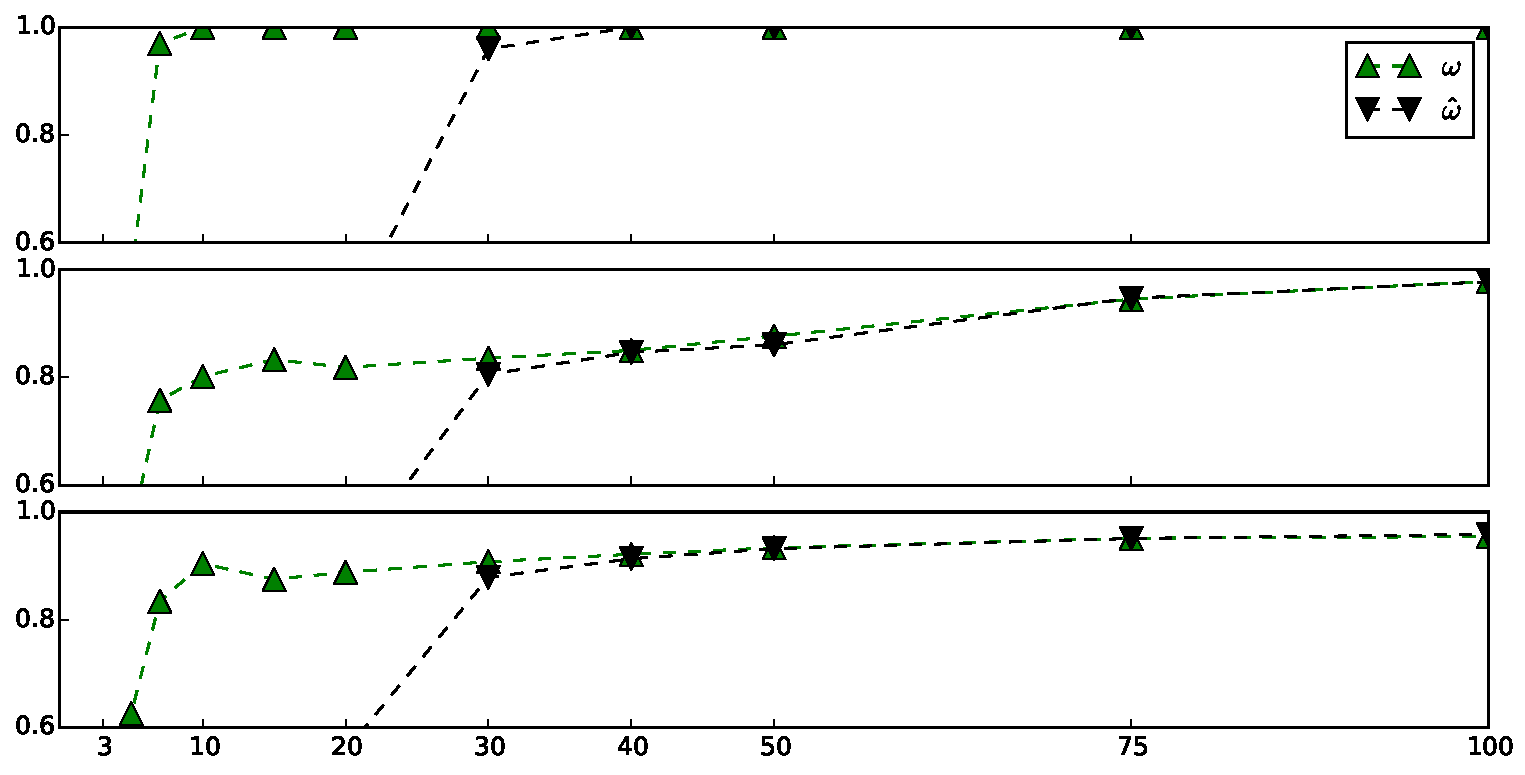
\includegraphics[width=\linewidth]{figures/ecai_estimation_omega.pdf}
%\end{figure}
%We can see that the estimation $\hat{\omega}$ converges to $\omega$ when $S$ is
%big enough. For small values of $S$, this estimation is indeed imprecise as it
%is difficult to find a lot a 3-tuples such that an analogical proportion holds
%for every element.

\section*{Conclusion}

In this Section, we have provided a functional and unifying definition of
analogical learners, which turned out to be closely related to the $k$-NN
classifiers. Starting from this definition, we were in a position to
prove an analytical convergence result, similar to that of the nearest neighbour
algorithm. Obviously, this is not enough to conclude regarding the predictive
ability of analogy-based classifiers. We have also shown that their
VC-dimension is infinite. It should not come as a surprise, as a very
particular case of analogical rule (when the analogical proportion is trivial)
is the $k$-NN rule.

This fact obviously has a consequence on the way we can
work to improve analogy-based classifier.  Indeed, learning by analogy is prone
to over-fitting and a relevant learning strategy should take this fact into
account.  Nevertheless, we have to keep in mind that the VC-dimension
alone is not a perfect marker of the quality of a machine learning algorithm,
especially when it comes to practical implementation.

In terms of accuracy in a Boolean setting, we have found a strong link between
the accuracy of the NAN algorithm and that of the NN algorithm. Our functional
definition tells us that we can consider the NAN algorithm as a NN strategy on an
extended and noisy training set: the analogical extension $\esf$. This leads us
to consider analogical classification as a two-steps process:
\begin{itemize}
  \item First, the training set is extended to the analogical extension
  \item Then, a $k$-NN algorithm is used on this extended training set.
\end{itemize}
Obviously, the accuracy of the NAN algorithm depends on the quality of the
analogical extension. In Chapter \ref{CHAP:analogy_preserving_functions}, we
will entirely describe the conditions needed for this extension to be perfectly
sound.

We have to remember that analogical reasoning brings its whole power in the
case where few data are available. If a lot of data are available, it is very
likely that we have elements similar to the one at hand and, in that case, a
$k$-NN style reasoning is natural. In the opposite case, when we only have a
few relevant cases at hand, applying analogical proportion-based predictions
appears to be a meaningful option.

This concludes for now our investigations with analogical classifiers. We have
seen that they have so far mostly been used for natural language processing
tasks, or classification in Boolean settings. One of the main goal of this
thesis was to apply analogical proportion-based reasoning to concrete,
real-world applications. We have chosen to investigate the suitability of
analogical proportion in the design of recommender systems. This is the object
of the next two chapters.


\chapter{Background on recommender systems}
\label{CHAP:background_reco_systems}
\localtableofcontents*
\vspace*{\baselineskip}

\initial{I}n a world of information overload, automatic filtering tools are
essential to extract relevant information from basic noise
\cite{RecoSystemHandbook,AdoTuzIEEE2005}. In the field of e-commerce,
recommender systems play the role of search engines when surfing the entire
web: they filter available items to provide relevant suggestions to customers.
They help to answer questions as diverse as ``which movie to rent?", ``which
car to buy?" or ``which restaurant to try?". They do so by providing the user
with a list of recommendations.

We have seen in the previous chapter that analogical learners exhibit promising
results when compared to the $k$-NN algorithms in a Boolean setting. In chapter
\ref{CHAP:analogical_recommendation}, we will try to apply analogical learning
to a recommendation task to see if analogical learners can prove useful in
these more challenging contexts.

In this chapter, we will provide some necessary background on recommender
systems, before diving into Chapter \ref{CHAP:analogical_recommendation} where
we will describe our contributions and experiments. This chapter is structured
as follows. We first provide a taxonomy
of current research in the recommender systems area in Section
\ref{SEC:taxonomy_rec_sys}, and set ourselves within the collaborative
filtering framework. In Section \ref{SEC:recommendation_rating_prediction}, we
formally define the specific recommendation problem that we will address in
this document, and we explain how to assess the quality of a recommender system
in this context. In Section \ref{SEC:neighborhood_and_matrix_facto_review}, we
extensively describe two collaborative filtering methods: neighborhood-based
algorithms, and matrix factorization-based techniques. These two families of
algorithms will serve as baselines with which we will compare our own prediction
algorithms in Chapter \ref{CHAP:analogical_recommendation}.

\section{Taxonomy of recommender systems}
\label{SEC:taxonomy_rec_sys}

Undoubtedly, there are many different tasks that range among the general problem
of recommendation. If they all share the ultimate goal of providing users with
relevant recommendations, they greatly differ in nature by the items that are
recommended, and by the technical means that are involved.

To provide a clear view of the vast recommendation landscape, various taxonomies
for recommender systems have been proposed: see for example \cite{Bur02,
AdoTuzIEEE2005, Bur07}, and more recently \cite{BurRam11}. Using that of
\cite{BurRam11}, we will successively describe \textbf{content-based},
\textbf{collaborative} and \textbf{knowledge-based} approaches in the next
three sections, and show that they generally apply to different problems.

Rest assured that in real systems, the frontiers between these three families
are not that sharp, and practical recommendation solutions usually fall into
more than one single category. We refer to such systems as \textbf{hybrid}
recommenders.

\subsection{Content-based techniques}

The general idea of content-based algorithms is as follows: they try to recommend to a user some items that are
\textbf{similar} to those that the user has liked in the past. For example, if
the renting history of a user mainly contains science fiction movies, the aim
of the system is to learn these preferences and to recommend some other science
fiction movies to the user. We recommend \cite{LopGemSem11} for a recent
overview of content-based methods.

To find out similar items to those that a user has liked, these systems usually
rely on a similarity metric whose nature strongly depends on the representation
of the items. In large-scale online shopping systems, were items are extremely
diverse and abundant, a similarity measure between two items would for
example be the number of web sessions on which the two item pages have jointly
been visited (yes, this is the reason why some online systems will try to sell
you a fridge even though you just bought a brand new one). In systems were
items are more homogeneous, i.e. in a movie store system, more  sophisticated
approaches can be built relying on some metadata about the items (hence the
name \textit{content}-based). In the case of movies, the metadata could be for
example the genre, main actors, film director, etc.

As content-based techniques usually do not rely on a set of ratings to compute item
similarities, a nice resulting feature is that new items that have not yet been
rated by anybody can still be recommended provided that the items are properly
described (which is not necessarily easy, as we will see). This is not the case for a new user
though: as we have no information about the items this user may like, a
content-based recommender would not be able to output any prediction. These
techniques also stand out by their explanatory potential: the motto
``\textit{here are some items that are akin to those you liked}'' is perfectly
understandable and seems sound.  Recommender systems usually strive for
explanatory power, because it is recognized that when confronted with a given
recommendation, users are more likely to accept the recommendation if they
understand and acknowledge the underlying process.

However, content-based systems are prone to various behaviours that tend to make
them less competitive than collaborative filtering methods. The first obvious drawback, known as
the problem of \textit{limited content analysis}, is precisely the need to
describe items with metadata (remember our movie example with
genre, actors, etc.). Such descriptions can be extremely costly to acquire, and can only
capture a very limited subset of item features, which are not necessarily the
most important ones when it comes to the users personal tastes. Going back to
our science fiction fan, it could be plausible that the user has a strong
preference for the steampunk sub-genre, and yet is perfectly indifferent to the
superhero fiction movies, and both can still be considered as sub-genres of
science fiction. A system that could not distinguish these two kinds of movies
would fail to provide our steampunk fan with relevant recommendations.

Another well-known drawback of content-based recommenders is their tendency to
overfit and recommend only items that users may already know or do not need
anymore (such as a fridge!). The recommendations tend to lack in novelty,
surprise and diversity. Also, content-based systems tend to output much less
accurate predictions than the collaborative filtering methods (the way accuracy
is computed will be described in Section
\ref{SEC:Recommender_system_evaluation}). This is why collaborative filtering
methods have gained in popularity.

\subsection{Collaborative filtering}

The main idea behind collaborative filtering algorithms is to recommend items
to a user that other users with similar tastes have liked in the past. In its
most general form, collaborative filtering methods (also called social
filtering) try to model the social environment of users and to output
recommendations based on the behaviour of their peers.

Probably the most common way of modeling the social environment of a user is to
use historical transactions stored in the system, for example using user-item
ratings: two users are peers if their ratings are similar. If Bob and Alice
usually agree on their movie ratings, i.e. they like the same movies and
dislike the same movies, and if Alice has not seen a movie that Bob has liked,
then it will be recommended to Alice.

A main advantage of collaborative filtering methods over content-based ones is
that they do not require any item or user knowledge: only user-item feedback is
needed to output a prediction. Thanks to this, they also allow to build systems
that can deal with items of different natures. It is indeed plausible to
imagine a collaborative filtering system recommending both books and movies, on
the basis that users that love the same books usually like the same movies. As
books and movies cannot be described using the same set of features (even
though they are close), the use of content-based techniques would make the task
much more difficult, or would again require largely hand-crafted work.

The main advantage of collaborative filtering methods is also their main
weakness. Before they can become effective, these systems require a serious
amount of data (i.e. user-item interactions) to train a model or to use
heuristics efficiently. A side-effect is known as the cold-start problem: there
is no way to yield recommendations for new users that have no known ratings,
and the same goes for new items that nobody has rated.

All the recommendation algorithms that we will propose in this document are of
a collaborative nature. Section \ref{SEC:neighborhood_and_matrix_facto_review}
will be devoted to an overview of two main collaborative techniques: the
neighborhood approach and matrix factorization-based methods. They are
typical examples of the two main approaches to collaborative filtering:
heuristic-based systems, and model-based systems.

\subsection{Knowledge-based systems}

The two families we have described so far (content-based and collaborative
methods) are only suitable for certain kinds of items. While movies, books,
music or news can all fit quite well within these two frameworks, this is not
the case for some other items such as cars, bank loans, or real estates. Take
for example the problem of car recommendation. A content-based approach would
need to know what kind of cars the user has owned in the past, and would
recommend some new cars that are similar to those past vehicles. This method is
obviously bound to fail, not only because in practice such information about
past vehicles is never available, but also because the recommendations would be
based on some years-old preferences. As for collaborative methods, they would
require the system to have a massive amount of past transactions at its
disposal, and
people do not buy as many cars as they watch movies: only very few information
would be available, leading to disastrous results.

In broad terms, we refer to knowledge-based systems as any method that is
neither content-based nor collaborative. In general, these systems are used in
settings where the domain and contextual knowledge (i.e. the knowledge about the
items that are available in the system) prevails over any other source of
information, such as social information for example.

A practical instance of  knowledge-based recommendation takes the form of a
recommendation session, where users indicate their needs in an interactive
manner, and the systems tries to match these needs as best as possible to
provide useful recommendations. According to \cite{FelBur08}, there exist two
kinds of knowledge-based systems, that differ in the way recommendations are
computed. The first category is made up of the \textbf{case-based} systems.
Case-based recommenders obviously draw from research in case-base reasoning
described at the end of the first chapter, and computations are based on
similarities: the system will try to recommend items that are similar to an
ideal item expressed by the user's needs. In
this respect, case-based recommenders are close to the aforementioned
content-based systems. The second  kind of knowledge-based recommenders are the
so-called \textbf{constraint-based} systems (see \cite{FelFriJanZan11} for a complete
review). In such systems, users and items are described
by a set of properties, along with a set of constraints. In the car
recommendation example, an item constraint could for example express that a
convertible car should not possess a sunroof, and user constraint could state
that the car color should not be green. The problem of recommending an item to
a user then takes the form of a classical constraint satisfaction
problem.

We are well aware that these two definitions of case-based and constraint-based
systems are quite general and vague, but the fact remains that practical
implementation of such systems are so domain-dependent that it is difficult to
exhibit a clear unifying framework that would still be accurate.

Now that we have a clear overview of the various tasks that range among the
wide topic of recommendation, we will detail the recommendation problem that
will be addressed in the next chapter.

\section{Recommendation by rating prediction}
\label{SEC:recommendation_rating_prediction}

In this section, we formally define the recommendation problem that we plan to
address later in Chapter \ref{CHAP:analogical_recommendation}. We also describe
how to assess the quality of a recommender system.

\subsection{Problem formalization and notation}
Let $U$ be a set of users and $I$ a set of items. For some pairs $(u,i) \in U
\times I$, a rating  $\rui$ is supposed to have been given by user $u$ to express
their preferences towards the item $i$. The way the preferences are expressed
depends on the rating scale that is used, which can be of different nature.
According to \cite{SchFraHerSen07}, we can distinguish four different kinds of
rating scales:

\begin{itemize}
  \item It is quite common that  $\rui$ belongs to a \textbf{numerical} rating
    scale. A typical numerical scale is $[1, 5]$, where  5 means a strong
    preference for item $i$, 1 means a strong rejection, and 3 means
    indifference, or just an average.
  \item A sub-case of the previous scale is the \textbf{binary} rating scale,
    where ratings belong to $[0, 1]$. In this case, we associate the value $0$
    with the meaning \textit{dislike} and the value $1$ with the meaning
    \textit{like}.
  \item An extreme case is the \textbf{unary} rating scale, where a value of
    $1$ translates as a preference, but rejections (or dislikes) are not
    addressed.
  \item Sometimes, the rating scale can be considered as \textbf{ordinal},
    where the elements of the scale have no absolute meaning and are only
    meaningful when compared to others, e.g. $[$\textit{rejection, indifference,
    agreement}$]$.
\end{itemize}
In practice, these semantic distinctions are purely contextual: the
$[1, 5]$ rating scale could perfectly be interpreted as purely numerical,
or conversely as purely ordinal. This observation has been addressed for
example in \cite{KorSillRECSYS11}, and will also be discussed here in the next
chapter. However, the rating scale is a decisive component of a recommender
system, and algorithms are usually designed to work with only one single rating
scale.

Ratings may be collected in different ways, and we commonly distinguish explicit and
implicit ratings. \textbf{Explicit} ratings are those for which users have
explicitly expressed their preference towards the items. \textbf{Implicit}
ratings belong to a binary or unary scale, and correspond to the result of
collected data about users behaviour, without any active involvement. For
example, if a user has listened to a given track more than 10 times, we might
consider this as an implicit rating of $1$. The ability to deal with both
explicit and implicit ratings can lead to significant improvements for a
recommender system. In \cite{KorSillRECSYS11}, a model using only explicit
numerical ratings was extended to deal with implicit ratings, which notably improved
the RMSE of the system (defined later). When no implicit
ratings are available, the same authors showed that the simple modeling of
implicit ratings as $r_{ui}' = 1 \iff r_{ui} \in R$ led to significant
improvements. Here, $r_{ui}'$ is an implicit rating stating that $u$ has rated
$i$, regardless of the rating value.

In our work, we will mostly focus on the explicit and numerical rating scheme.
Also, the algorithms we will design will be of a collaborative nature, and
therefore they will rely on a dataset containing user-item interactions (in our
case, user-item ratings).
Let us denote by $R$ the set of known ratings recorded in the system. In real
systems, the size of $R$ is very small with regard to the potential number of
ratings which is $|U| \times |I|$, as a lot of ratings are missing. The set
$\Ui$ will denote the set of users that have rated item $i$, and $\Uij \eqdef
U_i \cap U_j$ is the set of users that have rated both items $i$ and $j$.
Similarly, $\Iu$ is the set of items that user $u$ has rated, and $\Iuv \eqdef
I_u \cap I_v$ is the set of items that both users $u$ and $v$ have rated.

A very common way of providing personalized recommendations to a target user is
to estimate their tastes regarding the items that the system provides. The taste of a
user $u$ for a given item $i$ is usually represented as the rating that $u$
would give to $i$.  Once these estimations are made, a simple option is to
recommend the items with the highest ratings among all the estimated scores for
the considered user (using the implicit assumption that a user should be
interested in the items with high scores).

More formally, a recommender system usually proceeds as follows:
\begin{enumerate}
\item Using a prediction algorithm $A$, estimate the unknown ratings $\rui$
  (i.e. $\rui \notin R$). This estimation $A(u, i)$ will here be denoted
    $\predrui$.
\item Using a recommendation strategy $S$ and in the light of the previously
  estimated ratings, recommend items to users. For instance, a basic yet common
    strategy is to suggest to user $u$ the items $i \notin I_u$ with the
    highest estimation $\predrui$.
\end{enumerate}

When using a unary or binary rating scale, these two stages are usually
indistinguishable: it is natural to recommend an item to a user if the
estimated predicted rating is $1$. In practice, the recommendation strategy
depends a lot on the pragmatic constraints of the system: a store manager may
want to push forward a given item to boost its sales, regardless of the
rating predictions outputted by the algorithm. As a result, most of the
research has focused on the prediction algorithms, and so will we. Note also
that this view is only meaningful for non-ordinal rating scale. When the output
of prediction algorithm $A$ are ranks, the recommendation strategy $S$ is
obvious and the distinction between $A$ and $S$ is superfluous.

Prediction algorithm implementations are strongly influenced by the fields of
data mining and of course machine learning. However, we want to emphasize that
the general setting of recommender systems is actually quite different from
that of classification or regression, the two main prediction tasks of machine
learning. A naive reasoning could lead us to consider that the rating
prediction problem with the rating scale $[1, 5]$ is nothing but a
classification task with five classes $1, 2, 3, 4, 5$. But this is forgetting
that the values $1, 2, 3, 4, 5$ are actually ordered, and that the difference
between \textit{class} $1$ and \textit{class} $2$ is not the same as the
difference between \textit{class} $1$ and \textit{class} $4$. But most
importantly, in classification or regression all the instances belong to the
same space (that space was $X^m$ in our previous chapters), and have the same
features. This is not the case here! In a recommendation problem, if we chose
our instances to be the users and their feature space to be the items, we would
end up with instances that are only \textbf{very partially described}, because of
course no user has rated the whole set of items. All the more, as the number of
items is usually very high, we would end up with a very high dimensional
problem, where traditional learning algorithms tend to fail due to the
so-called curse of dimensionality. Our point here is that recommender systems
problems do not really fit within the traditional machine learning setting, and
represent a new setting in their own right. It can be insightful to consider
our  prediction problem as that of matrix completion: the dataset $R$ can be
viewed as a sparse matrix $R \in \mathcal{M}^{\mid I \mid \times \mid U \mid}$ where columns are users and rows are items. Our
prediction task  is to fill-in the missing entries of this matrix.

We now describe how the quality of a prediction algorithm and of a
recommendation strategy can be evaluated.

\subsection{Recommender system evaluation}
\label{SEC:Recommender_system_evaluation}
Providing an accurate measure of the overall quality of a recommender system is
not a simple task, and diverse viewpoints have to be considered.
We can distinguish three main evaluation settings. The first one is to perform
\textbf{user studies}, where actual users are asked to interact with a given system and to
provide some feedback. This evaluation process is probably the one that allows
to best capture users need, because feedback is explicitly given. Naturally,
this is also the most expensive kind of experiment to conduct, because it
requires a lot of user time. The second evaluation setting is to perform
\textbf{on-line
studies}. In its most simple form, this is equivalent to A/B testing: to see
which of the two versions of our recommender performs better, we provide some
users with the first version (A) and some other users with the second version
(B). We
can then assess the change in performance between the two versions and decide
which one is the most suitable for our needs.

Finally, the last available option to evaluate recommender systems is to
perform \textbf{off-line evaluation}: in this setting, we dispose of a dataset of past
transactions (the set of all ratings $R$), and try to simulate user behaviour
to compute different measures.  In general, we will use $k$-folds
cross-validation procedures to reliably evaluate each of the performance
measures. The set of all ratings $R$ is divided into $k$ (typically $5$)
disjoint sets of equal sizes; at each of the $k$ iterations, the test set
$\Rtest$ is set to the $k^{\text{th}}$ subset and the training set
$\Rtrain$ is set as the union of the $k - 1$ remaining subsets: the system will
be trained on $\Rtrain$ and tested on $\Rtest$. The reported performances are
then averaged over the $k$ folds.

The first two evaluation settings (users studies and online studies) require
the use of an actual working recommender system. Thus, we will here only focus
on measures that can be calculated in an off-line evaluation process.

\paragraph{Accuracy\\}
The performance of the algorithm $A$ is usually evaluated in terms of accuracy,
which measures how close the rating predictions $\predrui$ are to the true
ratings $\rui$, for every possible prediction. The Root Mean Squared Error
(RMSE) is probably the most common indicator of how accurate an algorithm is,
and is calculated as follows:
$$\text{RMSE}(A) = \sqrt{\frac{1}{|\Rtest|} \cdot \sum_{\rui \in
\Rtest}(\predrui - \rui)^2}.$$

Another common indicator for accuracy is the Mean Absolute Error (MAE), where
important errors are not penalized more than small ones:
$$\text{MAE}(A) = \frac{1}{|\Rtest|} \cdot \sum_{\rui \in \Rtest}|\predrui -
\rui|.$$

As we said, RMSE probably is by far the most popular measure for
evaluating the performance of a recommender system. The simple fact that \$1
million was awarded for a 10\% improvement of RMSE during the Netflix competition
illustrates the supremacy of RMSE. Yet this measure is also criticized, if
only because it is not very easy to interpret it in a meaningful way: if you
end up with an RMSE of $0.5$, how do you know if it is good or not? You would
need to compare multiple algorithms before knowing what can be thought of as a
good RMSE, which by the way highly depends on  the rating scale.

Another issue with RMSE is that they do not properly reflect the way users
interact with a recommendation system \cite{JanResTuzZan16}.  Ultimately, the
most important feature of a recommender system probably is how well it can
\textbf{order} the different items for a given user, with regards to their
preferences. Indeed, it would be harmful to rank a disliked item higher than an
item for which the user has a strong preference, and conversely predicting a
rating $\predrui$ of $2.5$ while the true rating is $1$ (i.e. with a
potentially high error) is not as serious, because the corresponding item would
not have been recommended anyway.  The point here is that providing accurate
predictions is crucial, but only on a particular subset of predictions.

A related concern is that when using a suitable loss function, some algorithms
relying on an optimization process
can have a great RMSE score while still having no recommendation power.
As we will see, in Section \ref{SEC:experiments_clone}, a simple baseline
predictor  can outperform the RMSE of many other approaches, and yet this
algorithm has absolutely no recommendation power: the recommendations that it
outputs are the same for all the users.

To better reflect the user-system interaction, other precision-oriented metrics
are sometimes used in order to provide a more informed view.

\paragraph{Precision and recall\\}
Precision and recall help measure the ability of a system to provide relevant
recommendations, and are therefore indicators of the performance of the
recommendation strategy $S$. They are defined by means of the number of true
positives, true negatives, false positives and false negatives. As such, they
are mostly used in an implicit rating scheme (or at least with binary rating
scales), but they can also be used when the rating scale is gradual. In this
latter case, the recommendation strategy has to be clearly defined.

In the following, we denote by $I^S$ the set of items that the strategy $S$
will suggest to the users using the predictions coming from $A$. For
ratings in the interval $[1, 5]$, a simple strategy could be for example to
recommend an item $i$ to user $u$ if the estimation rating $\predrui$ is
greater than $4$:
$$I^S \eqdef \Set{i \in I | \exists u \in U, ~\predrui \geq 4,~ \rui \in \Rtest}.$$

We also define $I^*$ as the set of items that are \textbf{actually} relevant to
the users, i.e.  the set of items that would have been recommended to the users
if all the predictions made by $A$ were exact:
$$I^* \eqdef \Set{i \in I | \exists u \in U, ~\rui \geq 4,~ \rui \in \Rtest}.$$

\noindent
The \textbf{precision} of the
system is
defined as the fraction of recommended items that are relevant to the users,
and the \textbf{recall} is defined as the fraction of relevant recommended
items over all relevant items:
\begin{align*}
  \text{Precision} &\eqdef \frac{\mid I^S \cap I^*\mid}{\mid I^S \mid},\\
  \text{Recall} &\eqdef \frac{\mid I^S \cap I^*\mid}{\mid I^* \mid}.
\end{align*}

Precision and recall are complementary metrics: it would not make sense to
evaluate an algorithm performance by only looking at the precision, without
considering the recall. It is indeed quite easy to obtain a high recall (by
simply recommending all of the items), but that would lead to a terrible
precision. Precision and recall are commonly summarized into the
F-measure, which is their harmonic mean:
  $$
  \text{F} \eqdef 2 \cdot \frac{\text{Precision} \cdot
  \text{Recall}}{\text{Precision} + \text{Recall}}.
  $$

If accurate predictions are crucial, it is widely agreed that it is
insufficient for deploying an effective recommendation engine. Indeed,
other dimensions are worth estimating in order to get a complete picture of the
performance of a system
\cite{NeeRieKonACM2006,HerKonJohTerRieACM2004,KamBriRecSys2014}.  For instance,
one may naturally expect from a recommender system not only to be accurate, but
also to be surprising, and to be able to recommend a large number of items.

\paragraph{Coverage\\}
In its simplest form, coverage is used to measure the ability of a system to
recommend a large amount of items: it is quite easy indeed to create a
recommender system that would only recommend very popular items. Such a
recommender system would drop to zero added value. We here define the
\textbf{coverage} as the proportion of recommended items out of all existing
items ($I$):
$$\text{Coverage} \eqdef \frac{\mid I^S\mid}{\mid I\mid}.$$

\paragraph{Surprise\\}
Users expect a recommender system to be surprising: recommending an extremely
popular item is not really helpful. Be warned though: surprise is one of the
most difficult notions to grasp, especially when it comes to assess it with
numerical measures. Following the works of \cite{KamBriRecSys2014}, we will
here define the \textbf{surprise} associated with a recommendation with the
help of the pointwise mutual information (PMI). The PMI between two items $i$
and $j$ is defined as follows:
$$\text{PMI}(i, j) \eqdef -\log_2 \frac{P(i, j)}{P(i)P(j)} / \log_2 P(i, j),$$
where $P(i)$ and $P(j)$  represent the probabilities for the items to be rated
by any user, and $P(i, j)$ is the probability for $i$ and $j$ to be rated
together. They are estimated by $P(i) \approx \frac{\mid U_i \mid}{\mid U
\mid}$ and $P(i, j) \approx \frac{\mid U_i \cap U_j \mid}{\mid U\mid}$. PMI
values fluctuate between the interval $[-1, 1]$, $-1$ meaning that $i$ and $j$
are never rated together and $1$ meaning that they are always rated together.
To estimate the surprise of recommending an item $i$ to a user $u$, the authors
propose two definitions:
\begin{itemize}
\item either to take the maximum of the PMI values for $i$ and all other items
  rated by $u$, with $\surpmax(u, i) \eqdef \max\limits_{j\in I_u}
    \text{PMI}(i, j),$
\item
 or to take the mean of these PMI values with $\surpavg(u, i) \eqdef
    \frac{\sum_{j \in I_u} \text{PMI}(i, j)}{\mid I_u\mid }$.
\end{itemize}

The overall capacity of a recommender to surprise its users can be defined as
the mean of all the surprise values for each prediction. Because they are
defined using the pointwise mutual information, the \textbf{lower} the values
of $\surpmax$ and $\surpavg$, the most \textit{surprising} the recommendations.


\paragraph{Other dimensions\\}

There are  many other measures that can assess the performances of a
recommender system (see \cite{ShaGun11} for an extensive survey). We can cite
for example \textbf{trust} which characterizes the confidence that a user would
put into a recommendation, or also \textbf{diversity} that evaluates how
the recommendations are distinct from each other.  Unfortunately these
dimensions are actually a lot harder to assess in an off-line setting, and
there are no popular quantitative measure that can evaluate them in a
satisfactory way.

Now that we know how to evaluate the performances of a recommender system, we
will detail two very popular collaborative filtering algorithms that usually
lead to good results.

\section{Two collaborative filtering techniques: neighborhood-based, and matrix
factorization}
\label{SEC:neighborhood_and_matrix_facto_review}

We will here present two families of collaborative filtering algorithms: the
neighborhood approach based on the well known $k$-NN algorithm, and the matrix
factorization techniques whose groundings come from linear algebra and that
lead to elegant and accurate models. These two families of algorithms will
serve as baselines against which we will compare the performances of our own
algorithms in the next chapter, so it is important that we understand their
functioning in detail.

\subsection{The neighborhood approach}
\label{SEC:neighborhood_approach}

\subsubsection{Prediction framework}

The motto of collaborative filtering methods is to recommend some items that
are appreciated by other users having the same tastes. This principle is
carried out to the letter in neighborhood methods. Neighborhood approaches are instances of the general $k$-NN scheme. To estimate
the rating $\rui$ of a user $u$ for an item $i$, the most basic method consists
in computing  the set of $k$ users that are most similar to $u$ and
that have rated $i$. We will denote this set $N_i^k(u)$. The computation of
$N_i^k(u)$ depends of course on a similarity measure between users, which is
based on their respective ratings. The estimation $\predrui$ of $\rui$ is then
computed as an aggregate of the ratings $\rvi$, where $v$ is one of the
neighbors of $u$ in $N_i^k(u)$. Usually, the aggregation is simply a mean
weighted by the similarity between $u$ and $v$:

\begin{definition}[Neighborhood approach]
  The estimation of a rating $\rui$ using the \textbf{neighborhood approach} (also
  denoted $k$-NN here) is:
  $$\predrui = \frac{\sum\limits_{v \in N_i^k(u)} r_{vi} \cdot \text{sim}(u, v)}
  {\sum\limits_{v \in N_i^k(u)}\text{sim}(u, v)},$$
  where $N_i^k(u)$ is the set of users having rated $i$ and having the highest
  $k$ values of sim with $u$:
  $$N_i^k(u) \eqdef \Set{v \in U | \rvi \in R,~v\in \argmax_{u' \in
  U}^k\left[\text{sim}(u, u')\right]}$$
\end{definition}

The estimation process of the neighborhood approach is described in Algorithm
\ref{ALGO:neighborhood_prediction}.  Obviously, the training stage only needs
to be done once. Then, the
similarities can be reused for future predictions.

\begin{algorithm}[!ht]
 \caption{The neighborhood recommender.}
       \label{ALGO:neighborhood_prediction}
       \begin{algorithmic}

         \STATE {\bf Input}: A set of ratings $R$, and a pair $(u, i)$ for
         which $\rui$ is  unknown.
         \STATE {\bf Output}: $\predrui$, an estimation of $\rui$.
         \STATE \textit{Training stage:}
         \FORALL{$(u, v) \in U^2$}
         \STATE Compute $\ssim(u, v)$.
	    \ENDFOR
       \STATE \textit{Prediction stage:}
         \STATE $\text{denum} \leftarrow 0, ~ \text{num} \leftarrow 0$
         \STATE $U_i^s \leftarrow \text{Sorted}(U_i)$  // \textit{Sort by value of
         $\ssim$ with $u$, in decreasing order}.

         \FORALL {$v \in U_i^s[:k]$}
         \STATE \textit{I.e. for the  $k$ first users in $U_i^s$}
         \STATE \text{denum} \leftarrow \text{denum}  $ + \ssim(u, v)$
         \STATE \text{num} \leftarrow \text{num} $ + \rvi \cdot \ssim(u, v)$
         \ENDFOR

         \STATE $\predrui \leftarrow \frac{\text{num}}{\text{denum}}$
\end{algorithmic}
\end{algorithm}

We need here to make an important point: instead of recommending an item to a
user, we could perfectly recommend a user to an item, which is a symmetric and
equivalent point of view. The prediction $\predrui$ would be the exact counterpart of the one we
described above, but instead of considering similarities between users, we
would compute similarities between items:
$$\predrui = \frac{\sum\limits_{j \in N_u^k(i)} r_{uj} \cdot \ssim(i, j)}
{\sum\limits_{j \in N_u^k(i)}\ssim(i, j)}.$$
The set $N_u^k(i)$ is defined as the counterpart of the set $N_i^k(u)$.
We can interpret this prediction as an edge-case of content-based
recommendation: the items we are recommending to $u$ are
close to some other items that $u$ has already rated in the past, which is exactly what a
content-based recommender does. In this case though, we did not use any
metadata about the items, and  items where represented as vectors of ratings.

The choice between a user-based or an item-based recommendation mainly depends on
the system at hand. When the number of users is high with regard to the number
of items, computing similarities between items can help saving memory and
computation time, but it is also important to assess the potential number of
neighbors for any given $u$ or $i$: it is always more desirable to compute
similarities over a high number of ratings. Also, item-based methods are
more easily justified: when presenting a recommendation to a user $u$, it is
easier to explain how two items relate to each other rather than involving
other users that $u$ does not even know.

\subsubsection{The similarity measures}
\label{SEC:similarity_measures}

There are  many ways to define the similarity metric between two users (or
items).
One of the most common measure is the Cosine similarity.

\begin{definition}[Cosine similarity]
  The \textbf{Cosine similarity} between two users $u$ and $v$ is defined as:
$$
\text{Cosine sim}(u, v) \eqdef \frac{ \sum\limits_{i \in \Iuv} \rui \cdot \rvi}
{\sqrt{\sum\limits_{i \in \Iuv} \rui^2} \cdot \sqrt{\sum\limits_{i \in \Iuv}
\rvi^2}}.
$$
\end{definition}

Here, users $u$ and $v$ are considered as vectors in a vector space defined by
the items they have both rated (the set of common items is $\Iuv$). Their
Cosine similarity simply is the cosine of the angle between the two vectors. An
unnatural feature of this metric is that two vectors with (potentially
different) constant values will always have a similarity of $1$, because they
are collinear. For example if $u = (2, 2)$ and $v = (5, 5)$, $\text{Cosine
sim}(u, v) = \frac{20}{\sqrt{8}\sqrt{50}} = 1$, while one would expect $u$ and
$v$ to be quite different with regards to their tastes.

Such a flaw can be overcome using the Pearson similarity, which can be viewed as
a mean-centered version of the Cosine similarity.

\begin{definition}[Pearson similarity]
  The \textbf{Pearson similarity} between two users $u$ and $v$ is defined as:
$$
\text{Pearson sim}(u, v) \eqdef \frac{ \sum\limits_{i \in \Iuv}
(\rui -  \mu_u) \cdot (\rvi - \mu_{v})} {\sqrt{\sum\limits_{i
\in \Iuv} (\rui -  \mu_u)^2} \cdot \sqrt{\sum\limits_{i \in
\Iuv} (\rvi -  \mu_{v})^2}},
$$
where $\mu_u$ and $\mu_v$ are the average rating of users $u$ and $v$
respectively.
\end{definition}

One last similarity metric that we will use is the Mean Squared Difference
(MSD)\footnote{Strictly speaking MSD is actually a distance rather than a
similarity metric, so we could take its inverse.}:
\begin{definition}[Mean squared difference]
  The \textbf{Mean Squared Difference} between two users $u$ and $v$ is defined as:
$$\text{MSD}(u, v) \eqdef \frac{1}{|\Iuv|} \cdot \sum\limits_{i \in \Iuv} (\rui
- \rvi)^2.$$
\end{definition}

Notice that none of these metrics take into account the support between the two
users $u$ and $v$, i.e. the number of items that they have commonly rated. It
would be foolish to have the same faith in a similarity computed over hundreds
of common items as in a similarity computed only over a few items. This is why
in practice, it is common to give a higher weight to the similarities that have
a high support. Another option is to \textit{shrink} the similarity measure of
two users toward zero if their support is low:
$$\text{shrunk\_sim}(u, v) \eqdef \frac{\mid \Iuv \mid - 1}{\mid \Iuv \mid - 1
+ \lambda} \cdot \ssim(u, v),$$
where $\lambda$ is a sort of regularization constant. Such shrinkage technique
can be motivated by a Bayesian perspective, and usually leads to significant
improvements in the system performances. It only makes sense however for
similarity measures that are centered around zero, such as the Pearson
similarity. We will not consider shrinkage in any of our experiments.

\subsubsection{Similarity computation}

We will now describe how to practically compute these similarity metrics. We
see that all of the presented metrics rely on the set of common items $\Iuv$.
In practice, the explicit computation of this set for every single pair of
users can be very expensive, and naive algorithms lead to poor performances.
Consider for example the naive similarity computation of Algorithm
\ref{ALGO:naive_sim}.
\begin{algorithm}[!ht]
 \caption{A general naive algorithm for similarity computation}
       \label{ALGO:naive_sim}
       \begin{algorithmic}

         \STATE {\bf Input}: A set of ratings $R$.
         \STATE {\bf Output}: The similarity between all pairs of users.
         \FORALL{$u \in U$}
         \FORALL{$v \in U$}
         \FORALL{$i \in I_u$}
         \IF{$i \in I_v$}
         \STATE \textit{We know now that $i \in I_{uv}$, so we can use $r_{ui}$
         and $r_{vi}$ as we please, depending on the measure that is computed}.
         \ENDIF
        \ENDFOR
        \ENDFOR
        \ENDFOR
\end{algorithmic}
\end{algorithm}
In the worst case, we can consider that $\mid I_u \mid = \mid I_v \mid = \mid I
\mid$ for all $u$ and $v$, so the complexity of this naive algorithm is
$\mathcal{O}(\mid U \mid^2 \mid I \mid^2)$.

However, the complexity can be taken down by a great deal if we proceed in a
MapReduce fashion \cite{DeaGhe04}, as described in Algorithm \ref{ALGO:cosine}
which exemplifies how to compute the Cosine similarity.
\begin{algorithm}[!ht]
 \caption{Computation of the Cosine similarity.}
       \label{ALGO:cosine}
       \begin{algorithmic}

         \STATE {\bf Input}: A set of ratings $R$.
         \STATE {\bf Output}: \text{Cosine sim}(u, v) for all pairs of users.
         \STATE {\it Initialization ($n$  is defined as the number of users, i.e. $n
         = \mid U \mid$):}
         \STATE $\text{sim} = \text{null\_array}[n][n]$
         \STATE $\text{sum\_prod} = \text{null\_array}[n][n]$
         \STATE $\text{sum\_squ} = \text{null\_array}[n][n]$
         \STATE $\text{sum\_sqv} = \text{null\_array}[n][n]$
         \FORALL{$i \in I$}
           \FORALL{$u \in U_i$}
             \FORALL{$v \in U_i$}
              \STATE $\text{sum\_prod}(u, v) \pluseq \text{sum\_prod}(u, v) +
              \rui \cdot \rvi$
              \STATE $\text{sum\_squ}(u, v) \pluseq \text{sum\_squ}(u, v) +
              {\rui}^2$
              \STATE $\text{sum\_sqv}(u, v) \pluseq \text{sum\_sqv}(u, v) +
              {\rvi}^2$
             \ENDFOR
           \ENDFOR
         \ENDFOR
         \FORALL{$u \in U_i$}
           \FORALL{$v \in U_i$}
           \STATE $\text{sim}(u, v) = \frac{\text{sum\_prod}(u,
           v)}{\sqrt{\text{sum\_squ}(u, v) \cdot \text{sum\_sqv}(u, v)}}$
           \ENDFOR
         \ENDFOR
\end{algorithmic}
\end{algorithm}
Actually, any other similarity measure that relies on the set $I_{uv}$ can be
computed this way (see \cite{SchBodVolRECSYS12}). Considering again the worst
case where $\mid U_i \mid = \mid U \mid$, the complexity of Algorithm
\ref{ALGO:cosine} is  $\mathcal{O}(\mid I \mid \cdot \mid U \mid^2 + \mid
U \mid^2) = \mathcal{O}( \mid U \mid^2 \cdot [ \mid I \mid + 1])$, which is far
less than that of Algorithm \ref{ALGO:naive_sim}. Another undeniable advantage
of Algorithm  \ref{ALGO:cosine} is that it follows the MapReduce framework, and
as such it can be easily parallelized for another significant performance gain.
Indeed, the first three embedded \texttt{for} loops could be dispatched in various
clusters, each dealing with a given set of items (this is the Map stage). Each
of the clusters would have its own three sum matrices \texttt{sum\_prod},
\texttt{sum\_squ} and \texttt{sum\_sqi}, which could then all be merged to
rebuild the entire sum matrices (Reduce stage). Let us note however that, even
if the similarities computation can be optimized in various ways, these methods
still become intractable when the number of users is too high, so other
methods are usually deployed.

That's all for the neighborhood methods. In the next section, we describe
another very popular collaborative filtering technique, which models the data
in a significantly different (but meaningful!) way: matrix factorization
techniques.

\subsection{Matrix factorization techniques}
\label{SEC:matrix_facto}

About ten years ago, the Netflix company organized a competition where the goal
was to improve the RMSE of their standard prediction algorithm by $10\%$. The
challenge quickly became very popular, not only because the winning prize was
of \$1 million, but also because the dataset was orders of magnitude larger
than any other available dataset at the time: about 100 million ratings from
480.000 users and 17.700 movies. Unfortunately, the dataset is no longer
publicly available, but the challenge led to the emergence of many successful
recommendation techniques, among which matrix factorization methods clearly
stand out. Let's be honest: the author of this document has a crush on matrix
factorization techniques, and as a consequence they will be thoroughly
detailed. All the more, just like neighborhood approaches, they have become one
of the main baselines for benchmarking.

The matrix factorization approach we will describe here is heavily inspired by
the Singular Value Decomposition (SVD) of a matrix, one of the highlights of
linear algebra. Because having a basic understanding of SVD will be very
insightful for us, we will briefly review it now.

\subsubsection{Background on SVD}

Let's first dive into the theory (but not for long):

\begin{proposition}
  Any real-valued matrix $R \in \mathcal{M}^{m \times n}$ of rank $r$ can be
  decomposed as the product of three matrices\footnote{The matrix $I$ is
  \textbf{not} the identity matrix!}:

  $$R = U\Sigma I^t,$$
  where $U\in \mathcal{M}^{m \times r}$, $\Sigma\in \mathcal{M}^{r \times r}$
  is a diagonal matrix, and $I\in \mathcal{M}^{n \times r}$. $U$ and $I$ are
  both \textbf{orthogonal} matrices, and this factorization is called the \textbf{Singular Value
  Decomposition} (SVD) of $R$.
\end{proposition}

In practice, we know how to compute the two matrices $U$ and $I$: their
columns are the
eigenvectors\footnote{For this reason, SVD and Principal Component Analysis are
strongly related.} of the two matrices $R^tR$ and $RR^t$, and their associated
eigenvalues are the squared entries of $\Sigma$, called the singular values
(hence the name of the factorization).
As $\Sigma$ is a diagonal matrix, it only acts as a scaling factor for either $U$ or
$I$. For the sake of simplicity, we will consider that the decomposition can be
written $R = UI^t$, where $\Sigma$ has been merged into either $U$ or $I$.

The key point is that the columns of $U$ are actually an \textbf{orthonormal
basis} for
the column space of $R$, and the columns of $I$ are an \textbf{orthonormal
basis} for the
row space of $R$. Maybe this statement is worth some explanation. The column
space of $R$ is the vector space that is spanned by the $n$ columns or $R$,
i.e. the set of vectors that are a linear combination of the columns of $R$. As
some of the columns of $R$ may be linearly dependent, this vector space is of
dimension $r\leq n$: the rank of a matrix is defined as the number of
independent columns, and equivalently as the number of independent rows. Our
statement says that the columns of $U$ span the columns space or $R$, and
particularly that they form an orthonormal basis of $r$ vectors for this vector
space. The same goes for the $r$ orthogonal columns of $I$, which span the row
space of $R$.

A particular case of this general statement is that \textbf{any column of $R$
can be expressed as a unique linear combination of the columns of $U$}. As the
columns of $U$ are orthonormal, each column has a unique contribution that
cannot be compensated by the others. Symmetrically, \textbf{any row of $R$ is a
linear combination of the orthogonal columns of $I$.} What does it have to do
with our recommendation problem? Imagine for a moment that $R$ is a dense
rating matrix, where the rows represent items and the columns represent users:
$$
R = \begin{blockarray}{cccc}
  \text{Alice} & \text{Bob} & \text{Charlie} \\
\begin{block}{(ccc) c}
  4 & 5 & 5 & \text{Titanic} \\
  2 & 1 & 1 & \text{Toy Story} \\
  1 & 2 & 2 & \text{LOTR} \\
  3 & 3 & 3 & \text{Mad Max} \\
  4 & 2 & 2 & \text{E.T.} \\
\end{block}
\end{blockarray}
=
\begin{pmatrix}
  \vertbar & \vertbar & & \vertbar\\
  U_1& U_2 & \cdots & U_r\\
  \vertbar & \vertbar & & \vertbar\\
\end{pmatrix}
\cdot
\begin{pmatrix}
  \horzbar& I_1 & \horzbar\\
  \horzbar& I_2 & \horzbar\\
   & \vdots & \\
  \horzbar& I_r &\horzbar \\
\end{pmatrix}
,
$$
where $U_1, \dots, U_r$ are the columns of $U$ and $I_1, \dots, I_r$ are the
columns of $I$ (i.e. the lines of $I^t$).

When we compute the SVD of $R$, we find in the columns of $U$ some
\textit{prototype} users that have no real existence, but that can be combined
(linearly) to build up any of the users: Alice, Bob and Charlie are linear
combinations of $U_1, U_2, \dots, U_r$. Also, any linear combination of Alice,
Bob and Charlie can be expressed as a linear combination of the $U_i$. Similarly, the columns of $I$ are
\textit{prototype} movies that do not properly exist but that can be combined
to build up Titanic, Toy Story, etc., and any of their linear combinations. We can consider each vector $I_i$
to be some sort of idealized movie type, for example $I_1$ is a typical action
movie, while $I_2$ would be a typical romantic movie, etc. Take the example of
Titanic, which is an \textit{action-packed romance} movie. Thanks to the SVD,
we can express Titanic  as a linear combination $\alpha_1 \cdot I_1 + \alpha_2
\cdot I_2 + \cdots + \alpha_r \cdot I_r$, and as $I_1$ and $I_2$ represent
typical action and romantic movies, the values $\alpha_1$ and $\alpha_2$
will be high. Also, if
$I_3$ is a typical science-fiction movie, $\alpha_3$ should be fairly low (or
even negative) for Titanic. The magic of SVD is that all these coefficients (or factors)
are automatically derived from the matrix $R$.

Similarly, the $U_i$'s can be viewed as some idealized critics, with specific
tastes toward some particular kind of movies. Obviously in practice, there is
no way to associate a clear semantic meaning to the different $U_i$ or $I_i$,
and the way they are defined only depends on the matrix $R$. We have here
chosen to interpret the prototype movies as \textit{action movie} or
\textit{romantic movie} for the sake of simplicity.

Moving further, let us now focus on the modeling of a single rating $r_{ui}$.
Each $\rui \in R$ is defined as a dot product $\rui =
{q_i}^t \cdot p_u$, where $q_i \in \mathbb{R}^r$ is a \textbf{row} in $U$ and represents
the item $i$, and $p_u \in \mathbb{R}^r$ is a \textbf{column} in $I^t$ and represents the
user $u$. We can now understand that \textbf{$p_u$ represents how well $u$
agrees with each of the $r$ prototype movies, and $q_i$ represents how well $i$
suits the tastes of the $r$ prototype users}.

\begin{testexample}
As an example, let us consider the rating of Charlie for Titanic. We will
assume that the rank $r$ is $3$ and that the three movies types are
\textit{Action}, \textit{Romance}, and \textit{Science fiction}. Charlie is a
guy who loves action movies and likes romantic movies, but does not like
science fiction at all. The two vectors $p_u$ and $q_i$ are described in Table
\ref{TAB:Charlie_Titanic}, and the rating $r_{ui}$ is high because Titanic
has all the attributes (or factors) that Charlie likes\footnote{These values
are completely arbitrary and obviously are not necessarily those that would
appear in the true SVD of $R$.}.
\end{testexample}

\begin{table}[h!] \centering \begin{tabular}{ l   c  c  c }
\toprule
    & Action & Romance & Science fiction\\
  \midrule
    Titanic $q_i$ & 1 & 3 & 0\\
    Charlie $p_u$ & 2 & 1 & -1\\
\bottomrule
\end{tabular}
  \caption{Charlie's rating for Titanic is ${q_i}^t \cdot p_u = 1 \cdot 2 + 3
  \cdot 1 + 0 \cdot (-1) = 5$.}
\label{TAB:Charlie_Titanic}
\end{table}

Here, each rating $\rui$ is a dot product between two vectors of dimension $r$,
because $U$ and $I$ are made of $r$ orthogonal column vectors. A strong result
related to SVD if we \textit{restrict} $U$ and $I$ to $U'$ and $I'$ with $f \leq
r$ columns vectors (choosing the $f$ vectors associated with the highest
corresponding values in $\Sigma$), the matrix product $U' {I'}^t$ is still a
good approximation of $R$. It is, in fact, the \textbf{best} approximation of
$R$ of rank $f$ with regards to the Forbenius norm\footnote{The Forbenius norm
of a matrix is the square root of sum of its squared entries.}.

\subsubsection{Application to recommendation}

The above statement is the principal motivation for the use of SVD in recommendation
settings. It postulates the existence of $f$ factors/criteria (whose nature is
not necessarily known) that determine the value of any rating $\rui$.  A user
$u$ is modeled as a vector $p_u \in \mathbb{R}^f$, where each component of
$p_u$ models the importance of the corresponding factor for $u$.  Similarly, an
item $i$ is modeled as a vector $q_i \in \mathbb{R}^f$, where each component of
$q_i$ models how well $i$ fits the corresponding criterion.  From then, a rating
prediction $\predrui$ is calculated as the dot product of the two vectors $p_u$
and $q_i$:
$$\predrui = {q_i}^t \cdot p_u.$$

Once the number of factors $f$ is set\footnote{$f$ must be lower than or equal
to the rank $r$. When $f < r$ we end up with a \textbf{low-rank} approximation
of the matrix $R$.}, the problem is here to estimate the
vectors $p_u$ and $q_i$ for every possible user and item. We saw that when the
matrix $R$ is dense (i.e. when  there is no unknown entry), there exists an analytic
solution for computing the two matrices $U$ and $I$. An equivalent solution is
to solve the following minimization problem\footnote{From then on we will abuse
notation and use $R$ both as a matrix (sparse or dense) and as a rating
dataset as defined in Section \ref{SEC:recommendation_rating_prediction}.},
with the constraint that the vectors $q_i$ must be orthogonal, as well as the
vectors $p_u$:
$$
\sum_{\rui \in R} \left(\rui - {q_i}^t \cdot p_u \right)^2.
$$

But what happens in a recommendation setting, where the matrix $R$ is extremely
sparse? The SVD of $R$ is not even properly defined! One of the main
contributions during the Netflix competition was made by Simon Funk in a blog
post\footnote{\url{http://sifter.org/~simon/journal/20061211.html}}, who empirically
showed that \textbf{we should actually just not care} that the matrix $R$ is
sparse, and still solve the same optimization problem only using the known
ratings.  When $R$ is sparse, the problem is not convex in both $p_u$ and $q_i$
so this optimization will only lead to a local minimum, but this method turned
out to be very efficient in practice. Before that, techniques usually involved  a
preliminary step where the matrix $R$ was filled using some heuristic, in order
to have a fully defined problem \cite{SarKarKonRie00}. Funk's contribution led
him to the top 10 competitors of the Netflix competition at the time, and was
heavily used by other competing teams, including the BellKor team that ended up
winning the contest \cite{Kor09}. It also turns out that the orthogonality
constraint is useful for interpretation purposes, but in practice it usually
leads to a lower generalization power, so we will simply not bother and allow
the factor vectors to be non-orthogonal.

The appeal of this basic approach does not only rest upon its link to SVD, but
also because it is easily extendable. It was later improved and theoretically
studied in many ways, for example by incorporating user and items biases
\cite{KorACM2010} (which we will further detail in Section
\ref{SEC:current_advances_neighborhood_techniques}), by adding the ability to
incorporate implicit ratings along with explicit ones \cite{Pat07, KorACM2010},
or by adding some time-dependent features, taking into account items popularity
over time \cite{Kor09}. Still in \cite{KorACM2010}, a model combining matrix
factorization techniques and neighborhood approaches was proposed. For a
complete overview mixing all previously mentioned methods, see \cite{KorBel11}
or \cite{KorBelVol09}.

In \cite{SalMni07}, the matrix factorization we just saw was studied from a Bayesian
perspective, and was named Probabilistic Matrix Factorization (PMF), leading to
the following regularized least squares problem:

$$
\min_{p_u, q_i}\sum_{\rui \in R} \left(\rui - {q_i}^t \cdot p_u \right)^2 +
\lambda\left(\norm{}{q_i}^2 + \norm{}{p_u}^2\right),
$$
where $\lambda$ is a regularization term. Not surprisingly, Stochastic Gradient
Descent (SGD) tends to perform really well when it comes to solving this
problem, and is quite simple to implement.  We have already talked too much
about matrix factorization, but a few lines more won't hurt so we now propose
to derive the associated SGD algorithm.

\subsubsection{Optimization by Stochastic Gradient Descent}

When we need to minimize a loss function $L$ of the form $L(\theta) = \sum_k
L_k(\theta)$, where $\theta$ is a (potentially multidimensional) parameter, SGD
comes up as a very popular optimization technique. While a vanilla gradient
descent would require to compute the derivative of $L$ with respect to
$\theta$, in SGD we just assume that the derivative of each $L_k$ is enough.
SGD is an iterative optimization process where the value of $\theta$ is updated
using the following rule: $\theta \leftarrow \theta - \alpha \frac{\partial
L_k}{\partial \theta}$, where $\alpha$ is the learning rate (or stepsize). This
update is performed over all $k$'s for a given number of times. Various
theoretical guarantees about the convergence of this algorithm have been
derived, that obviously depend on the stepsize and on some regularity
conditions on the loss function $L$: see \cite{BotCurNoc16} for a recent
overview.

As far as we are concerned, our loss function is:
$$
L(p_u, q_i) \eqdef \sum_{\rui \in R} \left(\rui - {q_i}^t \cdot p_u \right)^2 +
\lambda\left(\norm{}{q_i}^2 + \norm{}{p_u}^2\right).
$$
Let $L_{ui}$ be the cost associated with a single prediction $\rui$: $$L_{ui}
\eqdef \left(\rui - {q_i}^t \cdot p_u \right)^2 + \lambda\left(\norm{}{q_i}^2 +
\norm{}{p_u}^2\right).$$
Denoting $\text{err}_{ui}$ the prediction error ($\text{err}_{ui} \eqdef \rui
-\predrui \eqdef \rui - {q_i}^t \cdot p_u$), the
derivative of $L_{ui}$ with respect to $q_i$ is (remember that $q_i$ is a
vector):
$$\frac{\partial L_{ui}}{\partial q_i} = -\text{err}_{ui} \cdot p_u + 2\lambda
q_i.$$
Similarly, the derivative of $L_{ui}$ with respect to $p_u$ is:
$$\frac{\partial L_{ui}}{\partial p_u} = -\text{err}_{ui} \cdot q_i + 2\lambda
p_u.$$
With these derivatives in mind, the optimization problem can then be easily
solved by following Algorithm \ref{ALGO:matrix_facto_sgd}.
\begin{algorithm}[!ht]
 \caption{Stochastic Gradient Descent for matrix factorization.}
       \label{ALGO:matrix_facto_sgd}
       \begin{algorithmic}

         \STATE {\bf Input}: A set of ratings $R$, a learning rate $\alpha$, a
         regularization penalty $\lambda$ and a number of iterations $n$.
         \STATE {\bf Output}: $p_u$ and $q_i$, the user and item factors.
         \STATE {\it Initialization:}
         \STATE Randomly initialize $p_u$ and $q_i$
         \FOR{$\text{iteration} \in [1, n]$}
         \FORALL{$\rui \in R$}
         \STATE $\text{err}_{ui} = \rui - {q_i}^t \cdot p_u$
         \STATE $q_i = q_i - \alpha (\text{err}_{ui} \cdot p_u - \lambda q_i)$
         \STATE $p_u = p_u - \alpha (\text{err}_{ui} \cdot q_i - \lambda p_u)$
         \ENDFOR
         \ENDFOR
\end{algorithmic}
\end{algorithm}
Another optimization technique can be used, by noting that if either $p_u$ or
$q_i$ is fixed, we obtain a convex problem that can be solved using classical
least squares methods. The idea is then to first consider all $q_i$ as
constants and solve the associated linear problem. Then, the $p_u$ are
considered constant and the associated problem is solved. Repeating these steps
an arbitrary number of time will also converge to a local solution, and this
method is known as Alternating Least Squares \cite{BelKor07}.

\section*{Conclusion}

The purpose of this chapter was to provide the necessary background and tools,
in preparation for the next chapter where we will describe our contributions on
analogical recommendation.

We have seen that the three main families of recommender systems are the
content-based, collaborative and knowledge-based techniques. Collaborative
filtering is by far the most popular family of techniques today, so we will try
to address it in our contributions. In particular, we will try to
build algorithms that are capable of predicting the rating $\rui$ that a user
$u$ has given to an item $i$, on the basis of some past rating history.

We thoroughly detailed two popular collaborative filtering techniques. The
first one is the neighborhood-based method, which is a direct implementation of
the general $k$-NN strategy. The neighborhood of each user is computed using a
similarity metric that is based  on the ratings: two users are considered close
if they like the same items and dislike the same items. Then, the prediction
$\predrui$ is set as an aggregate (usually a weighted mean) of the ratings of
the neighbors of $u$ for the item $i$. The neighborhood-based methods tend to
model local relationship in the data. In contrast, the matrix
factorization-based techniques, whose popularity has grown during the Netflix
Prize, tend to model global effects in the data. These techniques define ratings
in terms of user and item factors. Each user $u$ is modeled as a vector of
factors which indicates how much the user likes the given factors.
Each item $i$ is also modeled as a vector of factors which indicates how well
$i$ corresponds to the given factors. The prediction $\rui$ is then set as the
scalar product between these two vectors, while the vectors are estimated using
a global estimation procedure (usually) based on stochastic gradient descent.
These two techniques (neighborhood and matrix factorization) will serve as
baselines in the next chapter to compare our algorithms performances.

We now have enough background on the recommender systems field to apply
analogical learning to a recommendation task. This is the purpose of the next
chapter.

\paragraph{Résumé du chapitre}

Nous avons vu dans le chapitre précédent que les classifieurs analogiques
proposaient des résultats prometteurs dans des domaines booléens,
comparativement aux classifieurs $k$-NN. Nous nous intéressons, dans ce
chapitre et dans le suivant, à l'usage de l'apprentissage par analogique à des
tâches plus concrètes, telles que celle de la recommandation.

Les systèmes de recommandation sont des outils de filtrage automatique qui
permettent de fournir des suggestions d'items aux utilisateurs d'un système.
Ils permettent de répondre à des questions aussi variées que ``dans quel
restaurant manger?'', ``quel film visionner?'', etc. Pour cela, les systèmes de
recommandation fournissent des listes de suggestions aux utilisateurs.
Le but de ce chapitre est de donner les prérequis nécessaires au sujet de
systèmes de recommandation, en vue du chapitre suivant où nous décrirons nos
contributions à la recommandation.

Nous avons vu qu'il existe trois familles principales de systèmes de
recommandation : les méthodes \textit{content-based}, les méthodes par filtrage
collaboratif, et les méthodes dites \textit{knowledge-based}. Le problème que
nous nous proposons d'étudier ici est celui de la prédiction de notes : étant
donné un ensemble de notes passées caractérisant les interactions d'un groupe
d'utilisateurs avec un groupe d'items, le but d'un algorithme de prédiction est
d'estimer les notes manquantes. Pour ce genre de problèmes, les systèmes
collaboratifs sont généralement nettement plus performants que les méthodes
\textit{content-based}. Nos contributions seront donc de nature collaborative.

Nous avons décrit en détail deux techniques populaires de filtrage
collaboratif. La première est la technique par voisinage, qui est une
généralisation directe des méthodes $k$-NN. Pour prédire la note d'un
utilisateur pour un item, le \textit{voisinage} de l'utilisateur est estimé,
puis on procède à une agrégation des notes des voisins pour l'item cible. Le
voisinage est généralement estimé à l'aide d'une mesure de similarité qui
caractérise à quel point deux utilisateurs ont tendance à noter les items avec
les mêmes notes. Ce genre de méthode a tendance à  modéliser des interactions
locales sous-jacentes aux données, contrairement aux méthodes par factorisation
de matrice qui modélisent des effets globaux. Les techniques par factorisation
de matrice modélisent les utilisateurs et les items comme des vecteurs de
\textit{facteurs latents}, lesquels sont estimés via un problème
d'optimisation. La note d'un utilisateur pour un item est alors donnée par le
produit scalaire entre leurs deux vecteurs respectifs. Ces deux familles de
méthodes (voisinage et factorisation de matrice) nous servirons à comparer les
performances de nos algorithmes dans le prochain chapitre.



\chapter{Analogical recommendation}
\label{CHAP:analogical_recommendation}
\localtableofcontents*
\vspace*{\baselineskip}

\initial{N}ow that we have enough background on recommender systems, we are in
a position to present our contribution to analogical recommendation.\\

This chapter is structured as follows. In Section
\ref{SEC:analogical_reco_basic_algo}, we will describe our first approach which is
directly inspired from extended classifiers, and compare it to the
neighborhood approach and matrix factorization-based techniques. In Section
\ref{SEC:clone_based_view} we will devise a new algorithmic framework that is still
inspired by analogy, but that does not rely on the search of $3$-tuples which
will appear to be very costly. Finally in Section
\ref{SEC:mining_analogical_proportions}, we will address the problem of mining
analogical proportions in partially described databases, and describe how the
solving of this problem can be applied to a recommendation task. This will also
help us to retrospectively analyze the results obtained in Section
\ref{SEC:analogical_reco_basic_algo}.

\section{An algorithm using arithmetic proportion}
\label{SEC:analogical_reco_basic_algo}
We will here describe our first attempt to use an analogical proportion-based
algorithm for recommender systems. Let us note that applying analogical
reasoning to the task of recommendation has already been addressed in
\cite{SakAkaOkaDatTakKamMiyTsu11}, though with a significantly different
concern. The main idea of our algorithm is quite
simple and is directly inspired by the analogical classifiers that we have
extensively studied in Chapter \ref{CHAP:functional_definition}.

\subsection{Algorithm}

Here again, we will make use of the analogical inference principle, but we will
state it in slightly different terms. In chapters
\ref{CHAP:formal_analogical_proportions} and \ref{CHAP:functional_definition},
the analogical inference principle stated that if four vectors $\mathbf{a},
\mathbf{b}, \mathbf{c}, \mathbf{d}$ are in proportion, then their labels should
also be in proportion.  Here, we will say that if an analogical proportion
stands between four users $a, b, c, d$, meaning that for each item $j$ that
they have commonly rated, the analogical proportion $r_{aj} : r_{bj} :: r_{cj}
: r_{dj}$ holds, then it should also hold for an item $i$ that $a, b, c$ have
rated but $d$ has not (i.e. $r_{di}$ is the missing component):
$$
\inferrule{r_{aj} : r_{bj} :: r_{cj} : r_{dj} ~~ \forall j \in
I_a \cap I_b \cap I_c \cap  I_d}
{r_{ai} : r_{bi} :: r_{ci} : r_{di} ~~ \forall i \in I_a \cap I_b \cap I_c,
\text{ and } i\notin I_d }
$$
This leads us to estimate $r_{di}$ as the solution $y$ of the following
analogical equation:
$$r_{ai} : r_{bi} :: r_{ci} : y.$$
Naturally, we may find many $3$-tuples $(a, b, c)$ that are in proportion with
$u$, so we will need  to aggregate all the candidate solutions $y$.  Given a
pair $(u,i)$ such that $\rui \notin R$, the main procedure to estimate $\rui$
is as follows:
\begin{enumerate}
\item Find the set of 3-tuples of users $a, b, c$ such that an analogical
  proportion stands between $a, b, c,$ and $u$ and such that the equation
    $r_{ai} : r_{bi} :: r_{ci} : y$ is solvable.
\item Solve the equation $r_{ai} : r_{bi} :: r_{ci} : y$ and consider the
  solution $y$ as a candidate rating for $r_{ui}$.
\item Set $\hat{r}_{ui}$ as an aggregate of all candidate ratings.
\end{enumerate}

This pseudo-algorithm is exactly that of a conservative classifier described in
Section \ref{SEC:conservative_classifier}, except that here, the instance space
(i.e. the space of $a, b, c, u$) changes with every pair $(u, i)$, and every
$3$-tuple $(a, b, c)$.

In our implementation, we have used the arithmetic proportion in
$\mathbb{R}^m$: $a:b::c:u \iff a - b = c - u$.  The four users $a, b, c, u$ are
here considered as vectors of ratings in a space defined by their common items.
For the sake of clarity though, we will not write them with boldface letters
and $a$ will denote both the user $a$ as well as its vectorial representation.
Let us consider Figure \ref{FIG:analogical_recommendation}: the four users $a,
b, c$ and $u$ are in proportion, i.e. they make up a parallelogram in the
2-dimensional space of their common items, namely the two movies Titanic and Toy story. If the
three users $a, b, c$ have rated a movie $i$ that $u$ has not rated, the
estimation of $\rui$ will be such that $a, b, c$ and $u$ still make up a
parallelogram, but this time in a 3-dimensional space. This process is also
explained in Table \ref{TAB:analogical_recommendation}.

\begin{figure}[!h]
\centering
  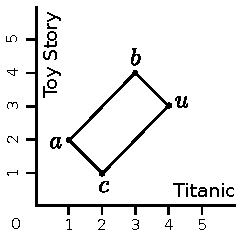
\includegraphics[width=2.5in]{figures/analogical_recommendation.pdf}
  \caption{Four users $a, b, c, u$ that are in proportion.}
\label{FIG:analogical_recommendation}
\end{figure}

\begin{table}[h!]
\centering
  \begin{tabular}{ c   c  c  c  c  c  }
\toprule
 & $j_1$ & $j_2$ & $j_3$ & $\cdots$ & $i$\\
  \midrule
$a$ & 1 & 4  & 3 & $\cdots$ & 2 \\
$b$ & 5 & 2  & 3 & $\cdots$ & 4 \\
$c$ & 1 & 5  & 3 & $\cdots$ & 3 \\
$u$ & 5 & 3  & 3 & $\cdots$ & ? \\
\bottomrule
\end{tabular}
\caption{The four users $a, b, c, u$ are in proportion for every item $j$ that
  they have commonly rated. For an item $i$ that $u$ has not rated, the
  prediction $\predrui$ is set as the solution of the analogical equation
  $2:4::3:?$, i.e. $\predrui = 3 - 2 + 4 = 5$, using the arithmetic proportion.}
\label{TAB:analogical_recommendation}
\end{table}

Just like with the conservative classifier, we will face the problem that in
practice, we may not find any $3$-tuple $a, b, c$ such that a perfect
proportion stands between $a, b, c$ and $u$. We will thus allow some distortion
of shape for the parallelogram $abcu$ by choosing another condition, for
example that $\norm{}{(a-b) - (c-u)} \leq \lambda$, where $\lambda$ is a
suitable threshold and $\norm{}{\cdot}$ is any $p$-norm. Let us notice that this
relaxing of the definition of an analogical proportion exactly corresponds to
the usage of an analogical dissimilarity, so technically our algorithm is very
close to that of an extended classifier.

Our analogical proportion-based algorithm for recommendation is described by
Algorithm \ref{ALGO:analogical_recommendation}.
 \begin{algorithm}[!ht]
       \begin{algorithmic}

      \STATE {\bf Input}: A set of known ratings $R$, a user $u$, and an item
         $i$ such that $r_{ui} \notin R$.
      \STATE {\bf Output}: $\hat{r}_{ui}$, an estimation of $r_{ui}$.

      \STATE {\bf Init}:
      \STATE $C = \varnothing$ \quad \quad // The set of candidate ratings
      \FORALL{
        users $a, b, c$ in $U_i$ such that:\\
        \begin{itemize}
        \item $\norm{}{(a-b)-(c-d)}\leq \lambda$
        \item $r_{ai} : r_{bi} :: r_{ci} : y$ is solvable
        \end{itemize}
      }

      \STATE  $y \leftarrow r_{ci} - r_{ai} + r_{bi}$
      \STATE $C \gets C \cup \set{y}$ \quad // Add $y$ as a candidate rating
	  \ENDFOR

         \STATE $\hat{r}_{ui} = \text{mean}_{y \in C} ~y$

\end{algorithmic}
     \caption{Analogical proportion-based algorithm for recommendation.}
       \label{ALGO:analogical_recommendation}
\end{algorithm}

We will note here an important point: while an extended classifier would look
for the $k$ $3$-tuples with the least values of analogical dissimilarity, we
here look for all $3$-tuples whose AD is below some given threshold. This is
a common variant of the $k$-NN algorithm: you can either look for the $k$
nearest neighbors, or look for all instances that are within a given distance.

We have considered a strict condition for the solvability of the equation
$r_{ai} - r_{bi} = r_{ci} - y$: as the exact arithmetic result $y=r_{ci} +
r_{bi} -r_{ai}$ does not necessarily belong to the rating scale used in our
experiments (which is $[1,5]$), we have considered that the equation is
solvable only when $r_{ai}=r_{bi}$ or $r_{ai}=r_{ci}$. In both cases, we ensure
that the solution $y$ is in $[1,5]$.  We also tried another option where an
equation is considered solvable when the solution belongs to $[1, 5]$. This
option led to extremely close results, where differences where not significant.

Just like for the neighborhood approach described earlier, it is perfectly
possible to apply this algorithm in an item-based way rather
than in a user-based way. I.e. instead of looking for $3$-tuples of users, we
may look for $3$-tuples of items.  As both methods lead to similar results when
compared to
the performances of the others recommendation algorithms, we
will only focus on the user-based approach described here.

In the next section, we will extensively study the performances of our
analogical recommender, and compare it to other standard recommendation
algorithms.

\subsection{Experiments and results}
\label{SEC:experiments_analogical_reco_basic}

The performances of our analogical recommender are summed up in Table
\ref{TAB:parall_performances_comparison}. Various options were considered, that
we will describe in a moment. We also report the performances of other standard
recommendation algorithms that we have already mentioned:
\begin{itemize}
  \item The basic neighborhood approach (denoted $k$-NN) with different
    similarity metrics, namely Mean Squared Difference, Cosine similarity and
    Pearson similarity.  For these three algorithms, the size of the
    neighborhood was set to $k=40$.
  \item The matrix-factorization algorithm (denoted PMF), as described in section \ref{SEC:matrix_facto}.
    The number of factors was set to $f = 100$, and the optimization problem
    was solved by a stochastic gradient descent of $20$ iterations with
    a constant learning rate of $0.005$ and a regularization penalty of $0.02$.
    These values are those recommended by the authors in \cite{KorBel11} for the
    Netflix dataset, and turned out to be quite efficient for our experiments.
  \item For the sake of completeness we also report results for an algorithm
    that always predicts the average of all ratings ($\predrui = \mu$ for all
    $u, i$). In addition, we also give the performances of a random algorithm
    that predicts random ratings based on the distribution of the dataset,
    which is assumed to be normal.
\end{itemize}

The reported metrics are RMSE, precision, recall, F-measure, coverage, and
surprise. Precision, recall, F-measure and coverage  are reported as
percentages. Remember that for these dimensions high values mean high
performance, while for RMSE and surprise low values are better.  RMSE is the
only measure that only depends on the prediction algorithm $A$. All the other
dimensions depend on the items that we actually choose to recommend, and
rely on the recommendation strategy $S$. Here, we have chosen to
recommend $i$ to $u$ if $\hat{r}_{ui} \geq 4$.

All reported results are averaged over a 5-folds cross-validation procedure.
Obviously, the $5$ folds are the same for all of the algorithms, to allow for
meaningful comparisons.  The dataset that we used is the MovieLens-100K
dataset\footnote{http://grouplens.org/datasets/movielens/}, composed of 100,000
ratings from 1000 users and 1700 movies. Each rating belongs to the interval
$[1, 5]$, and the sparsity of this dataset is of about 94\%, i.e. only 6\% of
all possible ratings are actually known. We also report the computation time of
each algorithm (roughly estimated), which is not an average but the total over
the $5$ folds. All our experiments have been carried out using Surprise
\cite{Surprise}, a Python recommendation library that we have developed
specifically for the occasion. The Surprise package will be described more in
depth in the conclusion of this chapter.

\begin{table}[ht]
  \centering
\begin{tabular}{ l  l l  l  l  l  l   l  l  l  l }
\toprule
  Algorithm & \multicolumn{2}{ l }{Details}  & RMSE & Cov &  Prec & Rec & F & $\surpmax$ & $\surpavg$ & Time \\
\midrule
  \multirow{4}{*}{Parall} & \multirow{2}{*}{Sample}& $n=100$ & 1.18 &  57& 95 & 68 & 79
                          & .419& .166& 10m \\

                          & & $n=1000$ & 1.04 & 23 & 95 & 27 & 42
                          & .418 & .168 & 1h\\

                          & \multirow{2}{*}{$k$-NN}& $k=20$ & 1.00 & 31 & 97 & 38 & 54
                          & .421 & .176 & 6h\\

                          & & $k=30$ & 0.99 & 25 & 96 & 31 & 47
                          & .422 & .177  & 19h\\
\cmidrule(lr){1-3}
  \multirow{3}{*}{$k$-NN} & MSD& $k=40$ & 0.98 & 23 & 96 & 28 & 43
                          & .423 & .175 & 30s\\
                          & Cos& $k= 40$& 1.02 & 21 & 96 & 26 & 41 &
                          .426 & .180 & 30s\\
                          & Pears& $k=40$ & 1.01 & 25 & 95 & 30 & 46 &
                          .425 & .170 & 30s\\
\cmidrule(){1-3}
                   PMF & & $f = 100$ & 0.95 & 38 & 99 & 47 & 64 &  .422 & .178 & 45s\\
                   Mean &  & & 1.13 &  &  &  &  &   & & 1s\\
                   Random &  & &  1.52& 81 & 86 & 89 & 88 &  .432 & .155 & 1s\\
\bottomrule
\end{tabular}
\caption{Performances of recommendation algorithms on the MovieLens-100k
  dataset.}
\label{TAB:parall_performances_comparison}
\end{table}

We have considered various alternatives for our analogical
recommender. In fact, when trying to predict a single rating $\rui$, looking
for \textbf{all} the $3$-tuples of users in $U_i$ as described in Algorithm
\ref{ALGO:analogical_recommendation} is simply impractical\footnote{Remember
that $U_i$ is the set of users that rated item $i$.}: there are often too
many users in $U_i$. As the complexity of this search is in $\mathcal{O}(\mid
U_i\mid^3)$ and as $\mid U_i\mid$ can be quite large for some items, strictly
sticking to Algorithm \ref{ALGO:analogical_recommendation} would lead to
even worse computation times. We thus have chosen two different strategies:
\begin{itemize}
  \item The first one is to randomly sample $n$ times a $3$-tuple in $U_i^3$.
    As in the strict version of Algorithm \ref{ALGO:analogical_recommendation}
    the prediction is an average from all the $3$-tuples in $U_i^3$, choosing a
    large value of $n$ should lead to a fairly good estimate. We have reported
    the results for $n = 100$ and $n = 1000$. Note though that $\mid U_i
    \mid^3$ is usually much larger than 1000, so we only have a very rough
    estimation here. This option is referred-to as \textbf{Parall Sample}.
  \item The second strategy is to consider the $3$-tuples $(a, b, c)$ in the
    neighborhood of $u$, using the assumption that the neighbors of $u$ are
    probably more reliable to yield a prediction where $u$ is involved. We have
    used the MSD metric to compute the neighborhood, and we have considered various
    sizes of neighborhood, namely $k = 20$  and $k = 30$. Unfortunately, values
    of $k$ greater than $30$ lead to basically never-ending algorithms. This
    option is referred-to as \textbf{Parall $k$-NN}.
\end{itemize}


\paragraph{RMSE analysis\\}

Out of all the algorithm, the PMF algorithm is by far the most
accurate, with an RMSE of 0.95. Matrix factorization  models were extremely popular during the
Netflix competition precisely because of their high accuracy. Note however that
even though the matrix factorization algorithms cannot be overlooked when it comes
to performance comparison, their philosophy remains quite different from that
of other classical neighborhood approaches. They tend to model data structures
at a high-level of abstraction, while neighborhood methods tend to model local
features of the data. As such, it makes more sense to compare the performances
of analogical recommenders to those of neighborhood-based techniques, rather
than use matrix factorization-based models as a baseline.

As expected, the RMSE of the
Parall Sample algorithm gets better while $n$ grows, but still
remains quite far from that of the $k$-NN algorithms. By paying attention to
the Parall $k$-NN algorithms, we see that looking for the
$3$-tuples in the neighborhood of the users significantly improves the
accuracy of our analogy-based algorithms. Their RMSE is better than that of the
neighborhood approaches when using Cosine and Pearson similarity, and it may
be expected that using a neighborhood size of $k=40$ would lead to an RMSE
close to that of the $k$-NN algorithm with MSD similarity.

\paragraph{Coverage\\}

Let us now consider the coverage measure. At first sight, it may appear that
the Random and Parall Sample 100 algorithm have the best recall values. But this
would be missing a very important detail: any measure that evaluates the
fitness of the recommendation strategy $S$ (such as the coverage) greatly
depends \textbf{also} on the fitness of the prediction algorithm $A$, simply
because $S$ highly depends on $A$. Therefore, the coverage of the Random
algorithm cannot be taken very seriously, because its accuracy (RMSE) is
disastrous: it  is only by chance that some items were estimated with a rating
greater than $4$, and were then recommended. The same goes for the Parall
Sample 100 algorithm, which has a quite bad accuracy.  Actually, the most
reasonable choice would probably the PMF algorithm again, which has the best
RMSE and very decent coverage. With respect to coverage, our other
analogy-based algorithms yield comparable performances to the
neighborhood-based methods, with a slight advantage for analogy-based methods.

\paragraph{Precision and Recall\\}

As for precision, recall and F-measure, we somehow have the same situation: the
Random algorithm seems to be the best one, but this need to be taken very
carefully. Here again, the PMF algorithm probably yields the best actual trade-off.
Comparatively, analogy-based algorithms have a slightly better F-measure than
the neighborhood approaches. This may describe the fact that our Parall algorithms
tend to produce more diverse recommendations, as would also suggest the results
on the coverage.

\paragraph{Surprise\\}
The surprise measures are a bit more tricky to analyze. Looking at $\surpmax$,
which assesses the least surprising recommendation (averaged over all users), we
see that the analogy-based algorithms tend to perform better, but the
$\surpavg$ measure counterbalances this observation. Undoubtedly, the surprise
associated to a recommendation remains an extremely tricky concept to grasp and
to model, and the measures presented here only allow to assess a very rough
aspect of this complex dimension.

\paragraph{Other remarks\\}

As a side note, we have reported only the RMSE for the Mean algorithm, because
this algorithm always outputs a prediction of $\predrui = \mu = 3.53$ which is
lower than the threshold we have chosen for our recommendation strategy $S$.
Therefore, not a single item is recommended with this algorithm, and the
precision, recall, etc. are not defined (or simply 0).

We are now led to computation time... The nightmare of every analogical
proportion-based algorithm. All of the other algorithms can manage through the
$5$-folds cross-validation procedure in less than a minute, but our
analogy-based algorithms need hours to yield only decent performances. This
issue is linked to the cubic complexity of the analogy-based learners, which
cannot cope with big amounts of data. For now, this limitation prevents
analogy-based learners to be relevant in real-world applications such as
recommender systems, where computation time is one of the most decisive
factor.\\

Nonetheless, it is still possible to design analogy-inspired solutions for
recommendation. In the next section, we describe other algorithms that rely on
the concept of \textbf{\textit{clones}} and that generalize the classical neighborhood
approach.

\section{A ``clone''-based view of analogical recommendation}
\label{SEC:clone_based_view}

Considering analogies between four users has shown to be computationally
intensive, thus not really suitable for recommendation purposes, where time is
a highly critical dimension. Yet, other forms of analogy can be addressed in
the recommendation task, based on the observation that some users may be more
inclined to give good (or bad) ratings than others. Indeed, ratings are in no
way absolute and greatly depend on the subjective appreciation each user has
about the rating scale. In the $[1, 5]$ scale for example, two users $u$ and
$v$ might semantically agree on an item $i$ describing it as $bad$, but there
is a chance that this agreement is not perfectly reflected in the ratings: $u$
might have rated $i$ with $r_{ui} = 1$ and $v$ with $r_{vi} = 3$, simply
because from $v$'s point of view $3$ is a \textit{bad} rating, while for $u$ a
rating of $3$ would simply mean \textit{decent} or \textit{good enough}.  In
the following, we refer to such users that \textit{semantically} agree on their
common items (but not necessarily \textit{numerically}) as \textbf{clones}, as
illustrated in Figure \ref{FIG:alice_and_bob_clones}. Please note that the word
$clone$ is not used here to mean \textit{strictly identical}, but rather in the
sense that two clones are two users following parallel paths.

\begin{figure}[!h]
\centering
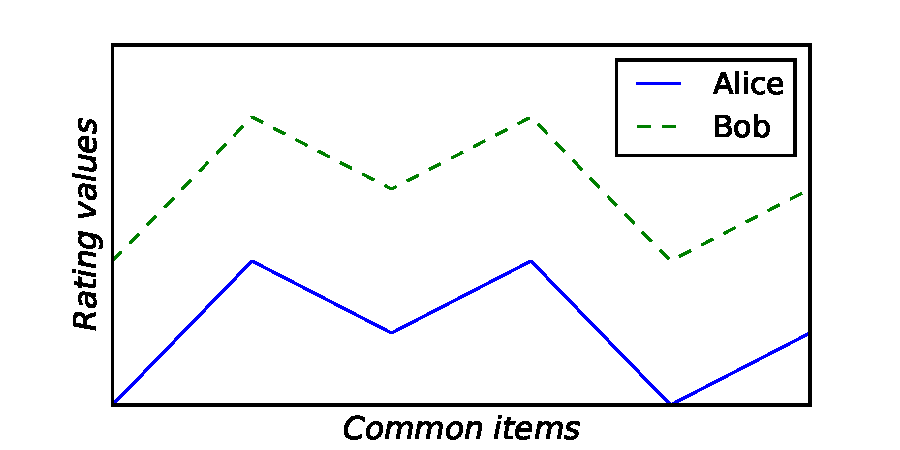
\includegraphics[width=4in]{figures/clones.pdf}
\caption{Bob is a perfect clone of Alice, and Alice is a perfect clone of Bob.}
\label{FIG:alice_and_bob_clones}
\end{figure}

It is obvious that in collaborative filtering, clones are of great interest
when it comes to predicting a user's ratings, and yet the information they provide
are often discarded. Indeed, in Figure \ref{FIG:alice_and_bob_clones}, Alice and
Bob would definitely not be considered as neighbors, so Bob would not be used to
predict Alice's ratings, and Alice would not be used to predict Bob's ratings.
The principle underlying the analogical clone-based view is the following: for
predicting a missing rating for $u$, we not only look at its nearest neighbors
but also at the users $v$ whose ratings are such that $r_{ui} = r_{vi} + t_{vu}$
where $t_{vu}$ is a more or less constant \textbf{correction term} that can be
either positive or negative. This correction term is the difference between
Bob's ratings and those of Alice. When two users $u$ and $v$ are clones, we can
come back to an analogical proportion-based viewpoint by noticing that we have:
$$r_{ui} : r_{vi} :: r_{uj} : r_{vj},~~ r_{uj} : r_{vj} :: r_{uk} : r_{vk},
\dots$$
where $i, j, k, \cdots$ are the common items rated by $u$ and $v$. The algorithms we
will derive will however be much more efficient than those of the previous
section, because they will not rely on an extensive search of 3-tuples of
users.


\subsection{Two new analogical algorithms}

In the following, $C_i(u)$ will denote as the set of users that are clones of
$u$ and that have rated item $i$. From the previous informal definitions, one
can easily derive a very general collaborative filtering framework for
predicting a user's rating by taking into account its clones: $$\predrui =
\aggr{v \in C_i(u)}(r_{vi} + t_{vu}),$$
where $t_{vu}$ is a \textit{correction term} that we need to add to $v$'s
ratings so that they correspond to those of $u$. We clearly have a
generalization of the neighborhood approach defined in Section \ref{SEC:neighborhood_approach},
which could be rewritten as:
$$\predrui = \aggr{\begin{subarray}{l}v \in C_i(u),\\ t_{vu} = 0\end{subarray}}(r_{vi} + t_{vu}).$$

Following this general framework, one can construct a great variety of
algorithms with various level of complexity. In the next subsections, we will
propose a very straightforward algorithm, and a more efficient one.

\subsubsection{A straightforward prediction algorithm}
\label{STRAIGHTFORWARD}

We will here design a very basic clone-based algorithm, to show that even a
basic method can outperform the classical neighborhood approach.

Let us first introduce the notion of $t$-clone. In its most simple form, a
user $v$ can be considered to be a $t$-clone of $u$ if the ratings of $v$
exactly differ from those of $u$ by a constant term $t$:
$$
t\text{-}C(u) \eqdef \Set{v \in U | \forall i \in I_{uv},~ r_{ui} = r_{vi} + t}.
$$
From then on, computing $\predrui$ amounts to finding all the users $v$ that
satisfy this criterion, and computing an aggregation of their ratings for $i$,
which can simply be an average. We implemented this basic algorithm described
by Algorithm \ref{ALGO:bruteforce}, and referred to as \textbf{brute-force}.

 \begin{algorithm}[!ht]
   \caption{A brute-force algorithm for clone-based recommendation.}
       \label{ALGO:bruteforce}
       \begin{algorithmic}

      \STATE {\bf Input}: A set of known ratings $R$, a user $u$, an item
      $i$ such that $r_{ui} \notin R$.
      \STATE {\bf Output}: $\hat{r}_{ui}$, an estimation of $r_{ui}$.

      \STATE {\bf Init}:
      \STATE $C = \varnothing$ \quad \quad // list of candidate ratings
      \FORALL{ users $v \in U_i$}
        \FORALL{$t$}
          \IF{$v \in t\text{-Clones}(u)$}
          \STATE $C \gets C \cup \{r_{vi} + t\}$ \quad // add x as a candidate rating
          \ENDIF
        \ENDFOR
	    \ENDFOR
    \STATE $\hat{r}_{ui} = \aggr{c \in C} c$
\end{algorithmic}
\end{algorithm}

Of course, one may want to relax the definition of a $t$-clone, as the current
one is too strict and only very few users will satisfy this criterion. In our
implementation, we chose the following condition:
$$
t\text{-}C(u) \eqdef \Set{v \in U |  \sum_{i \in I_{uv}} |(r_{ui} - r_{vi}) -
t| \leq \mid I_{uv}\mid},$$
which amounts to accept $v$ as a $t$-clone of $u$ if on average, the
difference $|r_{ui} - r_{vi}|$ is equal to $t$ with a margin of $1$.
The values of $t$ clearly depend on the rating scale. The datasets on which we
tested our algorithms use the $[1, 5]$ interval, so possible values for $t$
that we have considered are integer values in $[-4, 4]$.

This is obviously a very rough algorithm, to which one could point out numerous
flaws. The first obvious one is its time complexity which is very high, but the
purpose of this brute-force algorithm is simply to show that even such a basic
clone-based approach can lead to better results than a basic neighborhood
method, as we will see in the experiments section.

\subsubsection{Modeling clones with the similarity measure}
Another option to consider clones is to use the well known neighborhood-based
formula, and capture their effects using an appropriate similarity measure.
Recall that the general neighborhood formula is as follows:

$$\predrui = \frac{\sum\limits_{v \in N_i^k(u)} r_{vi} \cdot \ssim(u, v)}
{\sum\limits_{v \in N_i^k(u)}\ssim(u, v)}.$$

We have seen that this formula is commonly used with classical similarity
metrics such as Pearson similarity, Cosine similarity, or inverse of MSD.
However, these similarities are not fully satisfactory when it comes to
clones. Indeed with these metrics, two users are considered to be close if
their common ratings are often the same, but two perfect clones $u$ and $v$
with a significant correction term $t_{vu}$ would be considered as being far from
each other, thus involving a loss of information.

We propose the following simple choice of metric to measure how two users
relate as clones:
$$\clonedist(u, v) \eqdef  \frac{1}{\mid I_{uv} \mid} \cdot
\sum\limits_{i \in I_{uv}} \left[(r_{ui} - r_{vi}) - \mu_{uv}\right]^2,$$
where $\mu_{vu}$ is the mean difference between ratings of $u$ and $v$:
$$\mu_{uv} \eqdef \frac{1}{\mid I_{uv}\mid}\sum_{i \in I_{uv}} (r_{ui} -
r_{vi}).$$

We can understand this distance in two ways:
\begin{itemize}
\item it can be regarded as the variance of the difference of ratings between
  $u$ and $v$,
\item or it can be regarded as a simple MSD measure (defined in Section
  \ref{SEC:neighborhood_approach}) to which the mean difference of ratings between $u$ and $v$ has
    been subtracted.
  \end{itemize}

As our measure $\clonedist$ is a distance, it needs to be turned into 
a similarity measure. A common choice is to take its inverse (while accounting
for zero division):
$$\clonesim(u, v) = \frac{1}{\clonedist(u, v) + 1}.$$

\noindent
Once we know how to find the clones of a user, it is easy to output
a prediction using the classical neighborhood approach:
$$\predrui = \frac{\sum_{v \in N_i^k(u)} (r_{vi} + \mu_{uv}) \cdot \clonesim(u,
v)}{\sum_{v \in N_i^k(u)} \clonesim(u, v)}.$$

This algorithm will be referred to as \textbf{Clone}. For the sake of completeness, we
also tried the same formula but with a more basic similarity metric that does
not care about clones: MSD.

\subsection{Current advances in neighborhood-based techniques}
\label{SEC:current_advances_neighborhood_techniques}

What we have seen so far in terms of neighborhood methods are the rough, basic
techniques that have existed for a long time. Actually, more sophisticated
approaches have been developed, in particular during the Netflix competition.
The one we will describe here has been popularized in \cite{BelKorSIGKDD2007},
and makes use of \textbf{baseline predictors}:
$$\predrui = b_{ui} + \frac{\sum\limits_{v \in N_i^k(u)} (r_{vi} - b_{vi})
\cdot \ssim(u, v)} {\sum\limits_{v \in N_i^k(u)}\ssim(u, v)},$$
where $b_{ui}$ is a baseline (or bias) related to user $u$ and item $i$. Its
expression is $b_{ui} = \mu + b_u + b_i$, where $b_u$ is supposed to model how
$u$ tends to give higher (or lower) ratings than the average of all ratings
$\mu$, and $b_i$ is supposed to model how $i$ tends to be rated higher or lower
than $\mu$. For example, if the mean of all rating is $\mu = 3$, and the
ratings of a user are $(2, 2, 1)$, its bias $b_u$ would be close to $-1$.

Baselines are computed by solving a regularized least squares problem:
$$\min_{b_u, b_i} \sum_{r_{ui} \in R} \left[r_{ui} - (\mu + b_u + b_i)\right]^2
+ \lambda \left(b_u^2 + b_i^2 \right),$$
which can be achieved efficiently by stochastic gradient descent, or
alternating least squares. The regularization terms are here to avoid
overfitting: they allow to give more confidence to biases that are computed on
a high number of ratings. In our previous example, the user had only rated $3$
items so we cannot reliably say that its real bias is close to $-1$.
The regularization term will allow to give a value closer to 0 for this user
bias.

As a side note, notice that this optimization problem has the same look as the
one we used for the PMF algorithm of Section \ref{SEC:matrix_facto}. In fact, the use of
baselines can be easily combined with the matrix factorization model, leading
to the following optimization problem:
$$\min_{b_u, b_i, p_u, q_i} \sum_{r_{ui} \in R} \left[r_{ui} - \predrui\right]^2
+ \lambda \left(\norm{}{q_i}^2 + \norm{}{p_u}^2 + b_u^2 + b_i^2 \right),$$
with $\predrui = \mu + b_u + b_i + q_i^tp_u$. This prediction algorithm is
called SVD \cite{KorBel11}, and is nothing but the PMF algorithm with user and
items biases. Its extension to handling implicit ratings is called SVD++
\cite{KorBel11}, but we will not describe it here.

In their work, the authors have used this particular similarity metric, that is
in perfect accordance with their prediction formula:
$$\text{sim}(u, v) = \frac
{ \sum\limits_{i \in I_{uv}} (r_{ui} -  b_{ui}) \cdot (r_{vi} - b_{vi})}
{\sqrt{\sum\limits_{i \in I_{uv}} (r_{ui} -  b_{ui})^2} \cdot
\sqrt{\sum\limits_{i \in I_{uv}} (r_{vi} -  b_{vi})^2}}.$$

It is simply a Pearson correlation coefficient, except that instead of
centering ratings with their averages, they are centered with the baseline
predictors. This seemingly simple tweak actually has various consequences that
are very interesting. An intuitive and illuminating way to look at this
algorithm as a whole is to see that it conceptually follows these steps:
\begin{enumerate}
  \item Compute $R'$, the set of all ratings normalized by the corresponding
    baselines: $r'_{ui} = r_{ui} - b_{ui}$.  $R'$ can be regarded as the set
    where all ratings are given from the same frame of reference (in this case
    $0$), thus
    discarding any bias coming from the users or from the items. In $R'$,
    ratings can then be considered as absolute, in the sense that they are not
    spoiled by the users' moods or the items inherent popularity.
  \item Using $R'$, compute similarities between users using the Cosine
    similarity (the Cosine similarity is the same as the Pearson correlation
    coefficient, except that quantities are not centered).
  \item Output a prediction using the basic neighborhood formula. As this
    prediction belongs to the same space of $R'$ where ratings have no bias, it
    needs to be transposed back to the space of $R$ for performance evaluation
    purposes. This is why $b_{ui}$ and $b_{vi}$ are added (or subtracted) in
    the prediction formula of $\predrui$.
\end{enumerate}
\noindent
In what follows, this algorithm will be referred to as $\knns$.

\noindent
It is very clear that the use of the baseline predictors and the use of
clone-based recommendation are motivated by the same reason: they both come
from the fact that users (and items) tend to interpret the rating scale
differently.  This means that $\knns$ implicitly takes the idea of clones into
account, and thus a form of analogical reasoning.  Differences and resemblances
of these two approaches will be discussed in the next section.

\subsection{Experiments and discussion}
\label{SEC:experiments_clone}

To assess the suitability of our clone-based view of recommendation, we have
evaluated the accuracy of the brute-force and Clone algorithms, and compared
them to the previously mentioned approaches: the basic neighborhood method
($k$-NN), and
the neighborhood method taking into account user and item biases ($\knns$). For
reasons that will become clear at the end of this discussion, we also evaluated
the Bsl algorithm, whose prediction is simply the baseline predictor, i.e.
$\predrui = b_{ui}$. The evaluation protocol is the same as that of Section
\ref{SEC:experiments_analogical_reco_basic}, i.e. results are averaged over a 5-folds cross-validation
procedure. In addition to the MovieLens-100k dataset presented earlier, we also
used the MovieLens-1M dataset containing 1 million ratings with 6000 users and
4000 movies.  For each of these algorithms, the number of neighbors or clones
used to output a prediction is $k = 40$, except for the brute-force algorithm
where the number of clones cannot be controlled. The RMSE and MAE of the
algorithms are reported on Table
\ref{TAB:clone_based_rmse_mae}.

\begin{table}[ht]
  \centering
  \begin{tabular}{ l  l  l  l  l l l }
\toprule
    & & &  \multicolumn{2}{ c }{ML-100k}  & \multicolumn{2}{ c }{ML-1M} \\
  \cmidrule(lr){4-5}
  \cmidrule(lr){6-7}
    Algorithm& Details  & & RMSE & MAE  & RMSE & MAE \\
\midrule
    $k$-NN & MSD & $k=40$&  .979 & .773 & .921 & .725\\
    Brute-Force &  & & .948 & .737 & & \\
  \cmidrule(lr){1-2}
    \multirow{2}{*}{Clone} & \clonesim & $k=40$& .936 & .733 & .899& .705\\
                           & MSD & $k=40$ &  .931 &  .732 & .897 &  .707\\
  \cmidrule(lr){1-2}
    $\knns$ & & $k=40$ & .921 & .721 & .869& .680\\
    Bsl & &  & .945 & .749 & .909& .719\\
\bottomrule
\end{tabular}
  \caption{RMSE and MAE of our clone-based algorithms on the MovieLens-100k and
  1M datasets.}
  \label{TAB:clone_based_rmse_mae}
\end{table}

It is very clear that even a very straightforward approach of the clone-based
recommendation principle significantly outperforms the most basic $k$-NN
algorithm, and thus validates the need to take into account biases between
users. The brute-force is however a lot heavier to compute, and thus not very
suitable for real world recommendation purposes (its performances on the
MovieLens-1M dataset simply could not be computed). The two other clone-based
algorithms, however, have the exact same complexity of any $k$-NN-based
algorithm, which is a significant improvement from the algorithm described in
Section \ref{SEC:analogical_reco_basic_algo}.\\

Our two Clone algorithms output (almost) exactly the same
accuracies. This may seem a bit surprising, because the Clone MSD algorithm
does not take into account clones in the similarity measure, and we would
expect it to yield a lower accuracy. But this result still gives a further
reason to consider clones as useful predictors: the only difference between the
Clone MSD algorithm and the $k$-NN MSD algorithm (whose accuracy is much worse)
is that in the prediction of Clone MSD, the mean differences $\mu_{uv}$ between
the ratings of $u$ and its neighbors are taken into account. If this
(seemingly) simple change can make such a significant difference in the
accuracies, this means that the way users relate as clones is an important
feature of the dataset and should not be ignored.

Performances of the Clone algorithms are close to those of the state of the
art $\knns$ algorithm, yet the difference is more striking on the MovieLens-1M
dataset. It is however important to understand that these algorithms differ on
the following points:
\begin{itemize}
\item The Clone algorithms do not address item bias, which is a significant
  drawback. It is not unreasonable to believe that incorporating item bias
  in the prediction would lead to better results.
\item There is a subtle yet meaningful difference of interpretation between the
  biases induced by both algorithms. In the Clone algorithm, biases are all
  pairwise, meaning that they involve two users, and they are computed on items
  that both users have rated. As for the $\knns$ algorithm, there is no such
  thing as a pairwise bias. Bias for a given user is computed using only its
  own ratings, and is a result of a global optimization problem involving the
  global mean of all ratings, which means that every single rating in $R$ has
  an impact on the bias. As baselines are computed on the whole training set,
    they tend to capture most of the noise when the training set gets bigger.
    This may explain why the difference between the Clone algorithms and
    $\knns$ is more striking on the MovieLens-1M dataset.
\end{itemize}

As previously mentioned in Section \ref{SEC:similarity_measures}, it is recommended to perform a
shrinkage on the similarity measure of algorithm $\knns$, in order to take into
account the number of common items between two users: the more items they
share, the more confident we are when computing their similarity
\cite{KorACM2010}. Such techniques can further improve both RMSE and MAE of the
algorithm.  Similarly, in the clone-based approach, it might be of interest to
discount clones that rely on a too small number of common items.\\

Leaving clones for a moment, let us focus now on the Bsl predictor. Bsl outperforms by far the RMSE of the
$k$-NN algorithm, and in fact if we go back to table
\ref{TAB:parall_performances_comparison} on page
\pageref{TAB:parall_performances_comparison}, we see that it outperforms also the
algorithms mentioned there. Yet, this algorithm is unable to output
personalized recommendations: all the recommendations would be the same for
\textbf{any} user! This is simply due to the fact that in the prediction
$\predrui = \mu  + b_u + b_i$, the only user-dependent factor is the term
$b_u$, which is the \textbf{same} in all the predictions regardless of the
item. The point of this remark is to exhibit one of the drawbacks of RMSE that
we already mentioned before: RMSE is not an appropriate measure when it comes
to assess user-system interactions.

Indeed, what ultimately matters is how well a recommender system can
\textbf{rank} the preferences of a user for all the items. Also, rather than
defining clones with the general numerical criterion ($r_{ui} = r_{vi} +
t_{vu}$), we may instead consider that two users are clones if they order their
common items in the same way. Back to Figure \ref{FIG:alice_and_bob_clones}, we
see that Alice and Bob are perfect clones and we actually do not need to know
the real rating values: only the order matters. The goal of the next section is
precisely to investigate this ordinal view of ratings, and to see how it can be
embedded in our clone-based framework.

\subsection{Towards an ordinal view of ratings}

We will here investigate if we can devise a counterpart of the numerical clone-based
approach, which would be compatible with an ordinal view of the ratings.
Indeed, an extreme way for unbiasing and comparing two sets of ratings is to
forget about their numerical values, and only consider their respective rankings. The
idea of viewing ratings in a ordinal manner is not new, and has been advocated
for example in \cite{KorSillRECSYS11}.  In this section, we will discuss an
ordinal counterpart of the analogical approach previously presented.
Analogical reasoning with ordinal data has first been proposed in
\cite{MicBarCAP09}, yet with a different concern.

\subsubsection{An algorithm for rank prediction}
Indeed, the idea that ``\textit{the rating of user $u$ for item $i$ is to the
rating of user $v$ for item $i$ as the rating of user $u$ for item $j$ is to
the rating of user $v$ for item $j$}'' may be understood  as well in an ordinal
manner. This leads to state that ``\textit{the relative ranking of item $i$
  among the ratings given by user $u$  is to the relative ranking of item $i$
  among the ratings given by user $v$ as the relative ranking of item $j$ among
  the ratings given by user $u$  is to the relative ranking of item $j$ among
the ratings given by user $v$}''.

This means that we need to compare the rankings given by two users $u$ and $v$
on their common items. In the following, $\rho_{ui}$ denotes the relative
ranking of item $i$ out of all the items rated by $u$. Our goal is to estimate
all values of $\rho_{ui}$, for any user and any item. The main steps of a
possible algorithm would be as follows:
\begin{enumerate}
  \item Compute similarities between users, based on their rankings. A very
    popular similarity ranking measure is the Spearman's rank correlation
    coefficient (or Spearman's rho), that will be described later.
  \item Compute an estimated rank $\hat{\rho}_{ui}$ as an aggregation of all the
    rankings $\rho_{vi}$ extracted from the $k$ nearest neighbors (using
    Spearman's rho as similarity):
    $$\hat{\rho}_{ui} = \frac{\sum\limits_{v \in N_i^k(u)} \rho_{vi} \cdot
    \ssim(u, v)}{\sum\limits_{v \in N_i^k(u)} \ssim(u, v)}.$$
\end{enumerate}

This is obviously very similar to the numerical clone-based approach described
before, but instead of predicting a rating, we output the prediction of a rank. This
approach is denoted as \textbf{RankAnlg}.

The computation of Spearman's rho takes into account the relative rankings of
the ratings, and is computed as follows:
$$
\text{Spearman}(u, v) \eqdef \frac{\mathop{\text{Cov}}\limits_{i \in I_{uv}}(\rho_{ui},
\rho_{vi})}{\mathop{\text{std}}\limits_{i \in I_{uv}}(\rho_{ui}) \cdot
\mathop{\text{std}}\limits_{i \in
I_{uv}}(\rho_{vi})},
$$
where Cov naturally stands for covariance and std is the standard deviation.
Spearman's rho is usually defined as a statistic for random variables, and we
here have translated it as a realization of this statistic in our
recommendation setting. A common issue when dealing with rankings is that there
may be ties in the data. Consider for example user $u$ from Table
\ref{TAB:rankings}, whose ratings are $1, 1, 2, 3, 3, 3$ for items $i_1, i_2,
i_3, i_4, i_5$ and $i_6$.
\begin{table}[h!]
\centering
  \begin{tabular}{ l  l  l  l  l  l  l }
\toprule
    & $i_1$ & $i_2$ & $i_3$ & $i_4$ & $i_5$ & $i_6$\\
  \midrule
    $r_{ui}$ & 1 & 1 & 2 & 3 & 3 & 3\\
    Raw rankings & 1 & 2 & 3 & 4 & 5 & 6 \\
    Processed rankings $\rho_{ui}$ & 1.5 & 1.5 & 3 & 5 & 5 & 5 \\
\bottomrule
\end{tabular}
  \caption{Values of $\rho_{ui}$ for the user $u$.}
\label{TAB:rankings}
\end{table}
As $i_1$ and $i_2$ have the same ratings, there is no reason to rank $i_1$
before $i_2$, or $i_2$ before $i_1$. The same goes for $i_4, i_5$ and $i_6$,
and this is why the first ranking option (raw rankings) is not a suitable one.
Instead, it is common to consider that the ranking of a given item is the mean
of the raw rankings for the items that share the same rating value. In our case,
$\rho_{u{i_1}} = \rho_{u{i_2}} = \frac{1 + 2}{2}$, and $ \rho_{u{i_4}} =
\rho_{u{i_5}} =  \rho_{u{i_6}} = \frac{4 + 5 + 6}{3}$.
This process leads to a better estimation of Spearman's rho, and is equivalent
to averaging over all possible permutations between the raw ranks of items with
equal ratings.



\subsubsection{Experiments}

We evaluated the performance of our algorithm and compared it to other
previously described approaches, using the exact same evaluation protocol as in
the previous sections. The MovieLens-1M dataset was not benchmarked, because
the computation of Spearman's rho was too computationally intensive on this
bigger dataset.

RMSE and MAE are good measure for evaluation rating prediction accuracy, but
are not suitable when it comes to evaluate rankings. A better measure is the
Fraction of Concordant Pairs (FCP), which evaluates the probability that given any two
items $i$ and $j$ rated by any user $u$, the system has correctly estimated
whether $u$ prefers $i$ over $j$, or the reverse. To compute the FCP, we need to
use intermediate measures. Following the notation of \cite{KorSillRECSYS11},
$c_u$ defines the number of concordant pairs for user $u$, and $d_u$ is the
number of discordant pairs. The FCP is then computed over all users as the
proportion of concordant pairs.

\begin{align*}
  c_u &\eqdef \Set{(i, j) \in I^2 \quad | \quad \predrui > \predruj \text{ and
  } r_{ui} > r_{uj}},\\
  d_u &\eqdef \Set{(i, j) \in I^2 \quad | \quad \predrui \geq \predruj \text{
    and } r_{ui} < r_{uj}},\\
  \FCP &\eqdef \frac{\sum\limits_{u \in U} c_u}{\sum\limits_{u \in U} c_u +
  \sum\limits_{u \in U} d_u}.
\end{align*}
Here, $\predrui$ may represent either a rating prediction or a ranking
prediction $\hat{\rho}_{ui}$.

Results are reported in table \ref{table:res100kRank}.
\begin{table}[!ht]
\centering
\begin{tabular}{ l l  l l }
\toprule
     & RankAnlg &  $k$-NN & $\knns$\\
\midrule
\FCP  &  .7063   & .7096 &  .7163   \\
\bottomrule
\end{tabular}
\caption{\FCP~ of our rank prediction algorithm on the MovieLens-100k
  dataset.}
\label{table:res100kRank}
\end{table}
Unfortunately, even a basic algorithm such as $k$-NN that was not designed for ranking
prediction performs better in terms of FCP. To explain this difference, one may
look at the distribution of average support over all the predictions, as shown
on figure \ref{FIG:support_spearman_MSD}. Between
two users $u$ and $v$, the support is defined as the number of common items
$|I_{uv}|$ which was used to compute the similarity between $u$ and $v$. For
a given prediction $\predrui$, the average support is the average of all the
supports $|I_{uv}|$ over all users $v \in N_i^k(u)$.

\begin{figure}[!h]
\centering
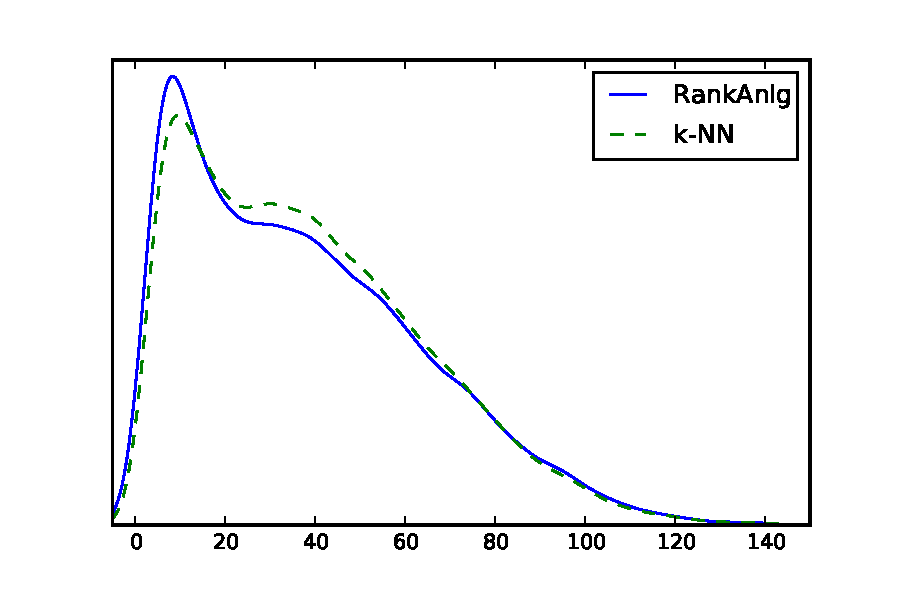
\includegraphics[width=2.5in]{figures/support.pdf}
  \caption{Distribution of average support for Spearman's rho (RankAnlg) and
  MSD ($k$-NN).}
\label{FIG:support_spearman_MSD}
\end{figure}

The use Spearman's rho tends to provide with neighbors that have smaller
support, thus leading to a less significant and less accurate estimation of the
neighborhood, which may explain the differences in performance.

This closes for now our contributions to analogical recommendation. We will
come back to it in the conclusion of this chapter, and we will now focus on a
somewhat unrelated problem: analogical proportion mining in databases. As we
will see though, analogical recommendation can in fact be viewed as both a
motivation \textbf{and} a purpose for the mining of analogical proportions.

\section{Mining analogical proportions}
\label{SEC:mining_analogical_proportions}

Let us recap a bit the first section of this chapter, where we described our
first attempt to design an analogical-based recommendation algorithm. As it is
a direct application of the analogical inference principle, our algorithm
suffers from the same drawbacks as the conservative and extended learners
introduced in Chapter \ref{CHAP:functional_definition}: the time complexity is
cubic, which makes it impossible to use in actual systems and hard to evaluate
accurately. Also, the performances of this algorithm were quite modest, even in
its most elaborated forms.

Our analogical inference principle used in the first section states that if
four users $a, b, c, d$ are in analogy, then their ratings for an item $i$ that
$d$ has not rated should also be in analogy:
$$
\inferrule{r_{aj} : r_{bj} :: r_{cj} : r_{dj} ~~ \forall j \in
I_a \cap I_b \cap I_c \cap  I_d}
{r_{ai} : r_{bi} :: r_{ci} : r_{di} ~~ \forall i \in I_a \cap I_b \cap I_c,
\text{ and } i\notin I_d }
$$
But we have so far neglected a central question: do such proportions actually
exist in our database? Can we find enough 4-tuples of users such that their
common ratings are in proportion? And if we can, how good are these proportions? We already
acknowledged that absolutely perfect proportions are actually hard to find, and
this is why we have relaxed the condition for an analogy to hold in Algorithm
\ref{ALGO:analogical_recommendation}.

In this section, we will design an algorithm that is able to answer all of
the above questions, by extracting all the analogical proportions underlying a
database that satisfy some given quality criterion. We will apply this algorithm
to the MovieLens database, and see how this relates to our recommendation task.
We will here look for analogies between items (movies in our case) instead of
looking for analogies between users, because the interpretation of a
movie-based proportion is actually easier, and because the parallel with
association rules (described below) will be more natural. Both problems are
symmetric though, and our solution can be adapted to user proportions in a
straightforward manner.

Because our method for mining analogical proportions is inspired from the mining
of association rules, we will first review this topic in the next subsection.

\subsection{Association rules}

Association rules are pieces of information that one can extract from a
database, and that reveal dependencies between items. Recommendation is one of
the principal application of association rules. Starting from the association
rule $i \implies j$, which means that users that buy $i$ tend to buy $j$ with
high probability, a recommendation system can suggest $j$ as soon as we bought
$i$ (but not yet $j$). A well-known example of association rule is the famous
$\text{beer} \implies \text{diapers}$ association, which was revealed after
mining association rules in a supermarket selling history, suggesting that
people tend to buy beer and diapers altogether. We now formally introduce the
problem of \textbf{association rule mining}.

Let $I = \Set{i_1, i_2, ..., i_m}$ be a set of $m$ items, and let $T =
\Set{t_1, t_2, ..., t_n}$ be a multiset of transactions, where each transaction
is a subset of $I$: $\forall i, ~ t_i \subseteq I$. A transaction simply is a set of items
that are purchased together. An association rule is expressed in the form $ X
\implies
Y$, where $ X \subset I, ~ Y \subset I$, and $X \cap Y = \varnothing$. $X$ and
$ Y $ are sets of items that we will call \textbf {itemsets}, and usually $Y$
is restricted to a single item. We define the \textbf{support} $\supp (X) $ of
an itemset $X$ as the proportion of transactions that contain it:
$$\supp(X) \eqdef \frac{\mid \Set{t \in T | X \subseteq t}\mid}{\mid T \mid}.$$
Sometimes, the support is not defined as a proportion but rather as the
absolute number $\mid \Set{t \in T | X \subseteq t}\mid$, but it only makes
sense to consider it with respect to the total number of transactions $\mid T
\mid$. Various
measures can be used to evaluate the quality of an association rule, such as
the \textbf{confidence} which can be expressed as:
$$\text{Conf}(X \implies Y)~\eqdef~\frac{\supp (X \cup Y)}{\supp (X)}.$$
As could be naturally expected, $\text{Conf}(X \implies Y)$ is equal to $1$
when the items of $X$ and $Y$ are systematically bought together, and decreases
if the set $X$ is sometimes found in a transaction that does not contain $Y$.

The mining of association rules is a popular research topic, and has been
extensively studied. In a perfect world with unlimited computational resources,
a naive association rules mining algorithm would be as follows:
\begin{enumerate}
\item First, generate the power set of $I$, i.e. the set of all subsets of $I$
  that we denote $2^I$.  We know that the elements in $2^I$ are partially
  ordered with respect to inclusion, and $2^I$ can be represented as a lattice
    where the \textit{join} is the union and the \textit{meet} is the intersection.
\item Let $I_S$ be any of the $2^m$ itemsets in $2^I$. Then for each $I_S$,
  compute all partitions $(X, Y)$ of $I_S$ and calculate the confidence
    associated with the rule $X \implies Y$. If the confidence is above a given
    threshold, then keep the association rule, else discard it.
\end{enumerate}

The second step remains reasonable and cannot really be optimized, but the
first one is obviously impossible to perform in practice due to the terrific size of $2^I$,
when real-world databases usually contain hundreds or thousands of items.
The most famous algorithm for association rule mining probably is the
\textbf{Apriori} algorithm introduced in \cite{AgrSriVLDB94}, that we will
briefly review. Using Apriori allows to scan the itemset lattice in an
efficient way, avoiding many useless nodes.

Ultimately, we are only interested in association rules where the support of
the involved itemsets is high. An itemset whose support is above some given
threshold $\alpha$ is called a \textbf{frequent} itemset. The downward-closure
property of support states that if $I_S$ is a frequent itemset, then all of its
subsets are also frequent itemsets. For example, if the itemset
$\Set{\text{apple, banana, orange}}$ is found in more than 30 transactions,
then the three subsets $\Set{\text{apple, banana}}$, $\Set{\text{apple,
orange}}$ and $\Set{\text{banana, orange}}$ must also be found in \textbf{at
least} 30 transactions. Conversely, if the two sets $\Set{\text{kiwi, pear}}$ and
$\Set{\text{kiwi, strawberry}}$ are found in less than $30$ transactions, we
are sure that their union $\Set{\text{kiwi, pear, strawberry}}$ will also be
found in less than $30$ transactions. So if we are only interested in itemsets
whose support is higher than $30$, there is no point in building the set
$\Set{\text{kiwi, pear, strawberry}}$, or any of its supersets.

Taking advantage of this fact, a basic version of the Apriori can be described
in the following steps:
\begin{enumerate}
  \item Consider all itemsets of size $1$ whose support is above $\alpha$.
  \item By joining these $1$-itemsets, build all possible $2$-itemsets and only
    keep those whose support is above $\alpha$.
  \item By joining these $2$-itemsets, build all possible $3$-itemsets and only
    keep those whose support is above $\alpha$.
  \item Etc, etc... All the frequent $k$-itemsets are built by joining the
    frequent $k-1$ itemsets.
  \item Once all the frequent itemsets have been computed, the second step of
    the above naive algorithm is used to assess the confidence of the
    association rules.
\end{enumerate}
In the end, we are provided with a set of association rules than comply with
some quality requirements, and that give us insightful information that link
the elements of our database.

%Sur le mode des proportions analogiques, on admettra que {\it le dentifrice
%est à la brosse à dent ce que le beurre est à la biscotte}.  Dans ce
%cas, on peut penser recommander à quelqu'un ayant acheté dentifrice,
%brosse à dent et beurre, d'acheter des biscottes. Sur quelle base?  Sur la
%base que la relation liant dentifrice et brosse à dent est la même que
%celle liant beurre et biscottes.

Just like association rules, the identification of analogical proportions in a
database is an additional information source, and deserves to be addressed. We
will now get to the heart of the matter.

\subsection{Looking for analogies in an incomplete database}

In order to avoid any ambiguity, we will formally define our problem first.
\subsubsection{Problem definition and links to association rules}

We will be looking for analogies between items in the MovieLens database, but
our method can naturally be extended to any other database with the same
structure.  We dispose of a set of users $U$ and a set of items $I$. Each user
$u$ has rated (or purchased) a given set of movies $I_u \subseteq I$. In this
setting, each user $u$ can be considered as a transaction $t$, as
defined in the previous section. The set of all the ratings $\rui$ is denoted
$R$ and can be viewed as a sparse matrix where users are columns and items are
rows (or the reverse).  For now, we do not care about the rating values and
just focus on whether the rating exists or not (just like we only care about
the fact that an item has been bought in the case of association rules). We
will only make use of the rating values when we will evaluate how good the
proportions are, in later subsections.

We need to insist here on the fact that we are dealing with a \textbf{sparse}
database.  In the case where all values in $R$ are known, the problem of mining
analogical proportion is pretty trivial: all we need is to look for all
$4$-tuples of items, and evaluate how good the proportion $a:b::c:d$ is. This
search is in $\mid I \mid^4$ which is absolutely awful, but there is simply no
other way around. This problem is not really interesting in the sense that
there is no need to come up with an elaborated algorithm. Its parallel in the
association rules world corresponds to the case where each transaction
$t_i$ contains all the items ($\forall i, t_i = I$): the very idea of
association rule does not make sense anymore. The problem we propose to address
here is different: the matrix $R$ is sparse and the set of users that have
rated (purchased) the items is different each time: for all items $i$ and $j$
(or at least for most), we have $U_i \neq U_j$. We thus cannot just look at all
$4$-tuples of items and check if they are in analogy. Or more accurately we
could, but as we are ultimately interested in good analogies (i.e. analogies
involving a sufficient number of ratings), we can make use of the
downward-closure property just like the Apriori algorithm, which will allow us
to avoid many $4$-tuples that could not lead to good analogies.

Let's now consider four users $a, b, c, d$, and our task is to find out if
these four users make up a valid analogy. For now, we do not know in which
order we need to consider them.  Just like for association rules, the notion of
support still makes sense here because these four users make up a $4$-itemset:
$$\supp(a, b, c, d) \eqdef \frac{\mid U_{abcd}\mid}{\mid U\mid},$$
where $U_{abcd}$ is the set of users that have jointly rated $a, b, c$ and $d$.
Here again, we will only be interested in proportions whose support is greater
than some threshold $\alpha$: a proportion built on only two components is a
lot less meaningful than a proportion built on dozens of components.

When given four items $a, b, c, d$, the question is now to find out which is
the proportion that actually holds. It could be $a:b::c:d$, but it could just
as well be $a:b::d:c$ or $a:c::d:b$, or any of the $24$ ($4!$) combinations of
these four elements. Fortunately, we do not have to test all the $24$
orderings.  We know from Chapter \ref{CHAP:formal_analogical_proportions} that
there are exactly 3 equivalent classes of analogies, which are represented by:
\begin{itemize}
  \item $a:b::c:d$,
  \item $a:b::d:c$,
  \item $a:d::c:b$.
\end{itemize}
Thus, testing these three orderings is enough to find out about the $24$
possible forms of analogies. To assess the quality of a proportion, we will
use a function $f$ that plays a similar role to the confidence function for
association rules. Then, it will be natural to only consider analogies that
are above some given quality threshold. Simply put, we would consider
$a:b::c:d$ as a valid analogy if $(a:b::c:d) \geq \beta$. In the end we are
left with a set of proportions that represent analogical relations between four
items.

\subsubsection{Assessing the quality of a proportion}

We will here describe various functions $f$ that can assess the quality of a
proportion. The four items $a, b, c, d$ are considered as vectors of ratings in
the space of their common users,
and we will consider two cases: that of the binary rating scale $[0, 1]$, and
that of the gradual rating scale $[1, 5]$. Note that here, in case of the
binary rating scale, the value $1$ is associated with \textit{like} and the
value $0$ is associated with \textit{dislike}, but a value of $0$
\textbf{still} means that the user $u$ has rated the item $i$. In some
settings (e.g. with the unary rating scale), a value of $0$ can be interpreted
as the absence of rating, but this view is not compatible with our problem: if
$\rui = 0$ means $\rui \notin R$, the four items $a, b, c, d$ would only be
represented as vectors of constant value $1$, where analogies are all trivial
because their only pattern is $1:1::1:1$. Instead, when $0$ still means that
the user has rated the item, the items can be represented as Boolean vectors,
which is fortunate because we know how to deal with Boolean proportions.

Naturally, the quality functions that we can define will depend on the nature
of the rating scale.

\begin{itemize}
  \item When we have a binary rating scale, the obvious choice for assessing
    the quality (or rather the \textit{badness}) of a proportion is the
    analogical dissimilarity defined in Section \ref{SEC:extended_classifier}. For Boolean
    vectors, the analogical dissimilarity is defined as the number of
    components that need to change in order to have a perfect proportion. Note
    however that we ultimately want to \textbf{compare} the quality of
    different proportions, and the fact is that no two $4$-tuples of items will
    have the same common users, so the item vectors of the two different
    $4$-tuples will likely have different dimensions. Therefore, it might be
    wise to consider the \textbf{relative} analogical dissimilarity, which is
    the classical AD divided by the dimension of the vectors.
  \item Another obvious quality measure in $\mathbb{B}^m$ simply is the number
    of components where a Boolean proportion perfectly holds. It is a slightly
    less conservative approach than the above one but still very similar. In
    practice, this means that the two proportions $0:1::1:0$ and $1:0::0:1$
    will be given an AD of $1$ instead of $2$. Here again, considering a
    fraction rather than an absolute number may be more meaningful, because
    of the different dimensions.
  \item When the rating scale is numerical (e.g. $[1, 5]$), the analogical dissimilarity is
    defined as $\norm{p}{(a - b) - (c - d)}$, and indicates how well the
    parallelogram $abcd$ holds. Clearly, this can also be used as a measure of
    quality of the proportion.
  \item Another option for the gradual rating scale is to use the definitions
    of the fuzzy analogy evaluation described at the end of Section
    \ref{SEC:formal_definitions_proportions}. As the quality of each proportion is
    evaluated in a component-wise fashion, we can choose various aggregation
    functions to assess the overall quality: mean, max, min, or also compare
    two proportions by lexicographic order. We will give further details in the
    experiments section.
  \item Finally, by adopting a statistical point of view, we can try to
    evaluate the probability of observing the proportion $a:b::c:d$, and
    consider it a meaningful proportion if it is unlikely that we could have
    observed this proportion by random chance alone. This method is highly
    linked to statistical test theory.
\end{itemize}

\subsubsection{Algorithm}

Our algorithm for mining analogical proportions imitates an association rule
mining process: we preliminarily set a threshold $\alpha$ for the support, and a
quality evaluation $f$ along with a threshold $\beta$.

After having built all the $4$-itemsets whose support is above the threshold
$\alpha$ with the Apriori algorithm, we compute the quality of the proportions
associated with the three equivalent classes, and keep those that satisfy our
criterion. These steps are described in Algorithm \ref{ALGO:proportion_mining}.

 \begin{algorithm}[!ht]
   \caption{Analogical proportion mining.}
       \label{ALGO:proportion_mining}
       \begin{algorithmic}

      \STATE {\bf Input}: A set of known ratings $R$, a quality function $f$,
         and two thresholds $\alpha$ and $\beta$.
         \STATE {\bf Output}: A set $\mathcal{P}$ of analogical proportions
         between items.
         \STATE $\mathcal{P} = \varnothing$
         \STATE \textit{Candidate retrieval:}
      \STATE Using Apriori, derive all the $4$-itemsets whose support is
         greater than $\alpha$.
         \STATE \textit{Quality evaluation:}
         \FORALL{$(a, b, c, d)$ in the set of $4$-itemsets}
         \FORALL {prop $\in \Set{(a:b::c:d), (a:b::d:c), (a:d::c:b)}$}
         \IF{$f(\text{prop)} \geq \beta$}
         \STATE $\mathcal{P} = \mathcal{P} \cup \Set{\text{prop}}$
         \ENDIF
         \ENDFOR
         \ENDFOR
\end{algorithmic}
\end{algorithm}

In theory, it is possible to end up with two non-equivalent proportions in
$\mathcal{P}$ that still relate to the same four items, i.e. we could find in
$\mathcal{P}$ the proportion $a:b::c:d$ as well as the non-equivalent
proportion $a:b::d:c$. It should not seem natural to have these two proportions
in $\mathcal{P}$, so if this happens, it is probably because the quality
function $f$ is too permissive or because the threshold $\beta$ is not
correctly tuned.

We also want to stress the point that the actual rating values are only used in
the second part of the algorithm, i.e. when we evaluate the quality of the
proportions. In the first part involving the Apriori algorithm, the only
information that matter are that a rating exists. Its value is not taken into
account.

\subsection{Experiments and discussion}

As previously indicated, we have considered the MovieLens-100k dataset for our experiments: 100,000
ratings in $[1, 5]$ from $1000$ users and $1700$ movies. We will first treat
ratings as numerical values, and in the second part of this investigation
we will binarize them.

\subsubsection{Numerical ratings}

For our purpose, we actually do not need to set a quality threshold $\beta$,
which would by the way be quite arbitrary. Instead, we will only be interested
in \textbf{comparing} the quality of the  proportions. We will not make use of
the analogical dissimilarity because the AD is dependent on the dimensions of
the vectors, and we will necessarily compare proportions that have different
dimension so this would not make sense. Instead, we have chosen to
compare two proportions by first computing the truth value of each of their
component-wise proportions using the graded-view of analogical proportions
described in Section \ref{SEC:formal_definitions_proportions}, and then by
comparing these truth values in lexicographic order. This allows to compare
proportions that have different dimensions in a more meaningful way.

This fuzzy view of analogical proportion is recalled here: for four real
elements $a, b, c, d \in [0, 1]$, the quality of the analogical proportion
$a:b::c:d$ is evaluated by:
\begin{align*}
A(a, b, c, d) =
\begin{cases}
  1 - |(a - b) - (c - d)| &\text{ if } a \geq b \text { and } c \geq d, \text{
    or } a \leq b \text{ and } c \leq d\\
  1 - \max(|a - b|, |c - d|) &\text{ if } a \geq b \text { and } c \leq d, \text{
    or } a \leq b \text{ and } c \geq d.
\end{cases}
\end{align*}

\begin{testexample}
Consider for example the two $4$-itemsets of Table
\ref{TAB:lexicographic_order}, where ratings $[1, 2, 3, 4, 5]$ have been mapped
to $[0, .25, .5, .75, 1]$. We will consider that the first $4$-tuple $i_1, i_2,
i_3, i_4$ (on the left) is a better proportion than the second one because
once their truth values are sorted, it is the one that comes first. Had we
chosen to compare them with the mean of the truth values, the best proportion
would have been the second one. In the remaining of this discussion, a
\textbf{component-proportion} will denote a proportion between ratings (for
example the proportion $0:1::0:1$ is the first component-proportion of
$i_1:i_2::i_3:i_4$), and in general a proportion  will refer to an analogy
between items (i.e. it is an aggregation of component-proportions).
\end{testexample}

\begin{table}[h!]
\centering
  \begin{tabular}{ c c  c  c  c }
\toprule
 $i_1 $ & $i_2$ & $i_3$ & $i_4$ & $A$\\
  \midrule
    0 & 1 & 0 & 1 & \textbf{1} \\
    0 & .5 & .25 & .75 & \textbf{1} \\
    1 & .5 & 1 & .25 & \textbf{.75} \\
    0 & .5 & 1 & .25 & \textbf{.25} \\
\bottomrule
\end{tabular}
\quad
  \begin{tabular}{ c c  c  c  c }
\toprule
 $i_5 $ & $i_6$ & $i_7$ & $i_8$ & $A$\\
  \midrule
    0 & 0 & 0 & 0 & \textbf{1} \\
    0 & .25 & 1 & .75 & \textbf{.75} \\
    1 & .5 & 1 & .25 & \textbf{.75} \\
    1 & 1 & 1 & .75 & \textbf{.75} \\
\bottomrule
\end{tabular}

\caption{Two $4$-itemsets and their related proportions, with corresponding
  truth value ($A$).}
\label{TAB:lexicographic_order}
\end{table}

Using this comparison procedure, we have looked for the 10 best proportions
with a minimum support of $200$ common users. The results are reported on Table
\ref{TAB:best_prop_num_basic_200}.
\begin{table}[h!]
\centering
  \begin{tabular}{l l  l  l l}
\toprule
    &\multicolumn{1}{c}{$i_1$}  & \multicolumn{1}{c}{$i_2$} &
    \multicolumn{1}{c}{$i_3$} & \multicolumn{1}{c}{$i_4$}\\
  \midrule
 1&   Star Wars & The Emp. Strikes Back & Raid. of the Lost Ark & Return of the Jedi  \\
 2&   Star Wars & Return of the Jedi & Raid. of the Lost Ark & The Emp. Strikes Back  \\
 3&   Star Wars & The Emp. Strikes Back & Return of the Jedi & Raid. of the Lost Ark  \\
 4&   Star Wars & Raid. of the Lost Ark & Return of the Jedi & I.J. and the Last Crus.  \\
 5&   Star Wars & Return of the Jedi & Raid. of the Lost Ark & The Fugitive  \\
 6&   Star Wars & Raid. of the Lost Ark & Return of the Jedi & Back to the Future  \\
 7&   Star Wars & The Emp. Strikes Back & Raid. of the Lost Ark & I.J. and the Last Crus.  \\
 8&   Star Wars & The Emp. Strikes Back & Return of the Jedi & I.J. and the Last Crus.  \\
 9&   Star Wars & The Emp. Strikes Back & I.J. and the Last Crus. & Return of the Jedi  \\
 10&   Star Wars & Raid. of the Lost Ark & The Emp. Strikes Back & The Fugitive\\
\bottomrule
\end{tabular}
\caption{The ten best item proportions with a support of more than $200$ common
  ratings, using $A$.}
  \label{TAB:best_prop_num_basic_200}
\end{table}

The first obvious observation is that only a few movies (exactly $7$) make up
these 10 proportions. This is not really surprising, as we have set the support
threshold quite high, and only a few movies are rated by more than 200 users.
In fact, we found 331 4-itemsets with more than 200 common users, but they only
contain 37 unique movies. Clearly here the involved movies (Star Wars, Indiana
Jones\dots) are extremely popular, and people tend to give them high ratings.
Using notions introduced in Section
\ref{SEC:current_advances_neighborhood_techniques}, we can say that these
movies have a high item bias $b_i$. To confirm this claim, we can check that in
average, the mean rating of these 7 movies is of 4.09, while the average rating
of all movies is only 3.53.

Some of the analogies are actually quite good though. For example the fourth
one \textit{Star Wars (1977)} is to \textit{Raiders of the Lost Ark (1981)} as
\textit{Return of the Jedi (1983)} is to \textit {Indiana Jones and the Last
Crusade (1989)}, or the seventh one which is similar: \textit{Star Wars (1977)}
is to \textit{The Empire Strikes Back} as \textit{Raiders of the Lost Ark
(1981)} is to \textit{Indiana Jones and the Last Crusade (1989)}

Looking at the first and third proportions, we see that the two forms
$i_1:i_2::i_3:i_4$ and $i_1:i_2::i_4:i_3$ are present in the table. These two
forms are non-equivalent, and it does not seem natural to consider these two
proportions as (almost) equally valid. But this result can be explained by
looking at the actual rating values: a great number of them are of the form
$r:r::r:r$ (where $r$ is usually a high rating, given that these movies are
popular). In the two cases, a switch between $i_3$ and $i_4$ has absolutely no
effect on the truth values of the analogies.

This leads us to another point: all these analogies are, after all, quite
trivial. They all concern quite similar movies. We do not mean to offend any
cinema fan, but we believe it is still fair to say that the differences between
a Star Wars movie and an Indiana Jones movie are quite shallow. And these
similarities are reflected in the ratings, where the most common pattern is
$r:r::r:r$ (or close to it), suggesting that people like all these movies the
same.

To try to discover some more surprising analogies, we basically have two
options. The first one is to tweak a bit our quality function $f$ (and in our
case, our comparison function) by penalizing proportions with the pattern
$r:r::r:r$, or inversely by promoting the proportions $r : r' :: r :r'$ where
$r$ and $r'$ are quite different. The second option is to lower the minimum
support threshold, to allow movies that are rated by a reasonable (and not
necessarily very high) number of users. As we have seen, movies with a very
high number of ratings are likely to lead to trivial proportions precisely
because they are popular, and because people like them all equally well in
general. If we really want to ban popular movies, we can also set a
\textbf{maximum} support threshold. This will also have the benefit to limit
the number of itemsets that we consider, leading to a significant improvement
in computation time. These two options will be explored.

\paragraph{Promoting \textit{disagreement} proportions\\}

Table \ref{TAB:best_prop_num_customTV_200} shows the 10 best proportions with a
minimum support of $200$, with a tweaked comparison function. Here, the truth
value of a component-proportion $r_1 : r_2 :: r_3 : r_4$ is defined by:
$$A'(r_1, r_2, r_3, r_4) = \frac{1}{2} A(r_1, r_2, r_3, r_4) + \frac{1}{4} |r_1
- r_2| + \frac{1}{4} |r_3 - r_4|.$$
We are here promoting proportions where rating values tend to disagree, which
should lead to different proportions from that of Table
\ref{TAB:best_prop_num_basic_200}. Proportions are still compared using the
lexicographic order of all the $A'$ values.
\begin{table}[h!]
\centering
  \begin{tabular}{ l l  l  l l }
\toprule
    & \multicolumn{1}{c}{$i_1$}  & \multicolumn{1}{c}{$i_2$} &
    \multicolumn{1}{c}{$i_3$} & \multicolumn{1}{c}{$i_4$}\\
  \midrule
    1& Star Wars  & Pulp Fiction  & The Empire Strikes Back  & The Fugitive   \\
    2& Star Wars  & Pulp Fiction  & Return of the Jedi  & The Fugitive   \\
    3&Star Wars  & Pulp Fiction  & The Empire Strikes Back  & The Silence of the Lambs   \\
    4&Star Wars  & Twister  & Return of the Jedi  & Independence Day  \\
    5&Star Wars  & Return of the Jedi  & The Silence of the Lambs  & Fargo   \\
    6&Star Wars  & The Terminator  & Return of the Jedi  & Pulp Fiction   \\
    7&Star Wars  & Pulp Fiction  & Return of the Jedi  & Terminator, The   \\
    8&Star Wars  & The Fugitive  & The Empire Strikes Back  & The Silence of the Lambs   \\
    9& Star Wars  & Pulp Fiction  & Return of the Jedi  & The Silence of the Lambs   \\
   10&Star Wars  & Pulp Fiction  & Raiders of the Lost Ark  & The Silence of the Lambs   \\
\bottomrule
\end{tabular}
\caption{The ten best item proportions with a support of more than $200$ common
  ratings, using $A'$.}
\label{TAB:best_prop_num_customTV_200}
\end{table}

We still have a lot of Star Wars movies (and a few Indiana Jones), but the
movies seem more diverse: we now have 11 unique movies, instead of just 7
before. 9 of these proportions comply with the pattern \textit{Star Wars
movie} is to \textit{Other Star Wars movie} what \textit{movie A} is to
\textit{movie B}. This suggests that we should find strong links underlying the
connection between \textit{Movie A} and \textit{Movie B}, because the two Star
Wars movies are deeply related. Is \textit{Pulp Fiction} related to \textit{The
Fugitive}? Is \textit{Twister} related to \textit{Independence Day}? Is
\textit{Fargo} related to \textit{The Silence of the Lambs}? We will not
venture to answer these questions, and leave them to the reader's appreciation.
All we can say is that some forms of analogy seem to emerge from their
respective ratings.  One thing we can note though, is that even though all these
movies are very popular just like in Table \ref{TAB:best_prop_num_basic_200},
their genres are however quite different: while we have considered Star Wars
and Indiana Jones to be of the same kind, we can fairly claim that a Star Wars
movie is very far from Fargo, Pulp Fiction or The Silence of the Lambs.

\paragraph{Lowering support threshold\\}

Table \ref{TAB:best_prop_num_basic_10_50} illustrates the ten best proportions
we have found after setting the minimum support at 10, and a maximum support at
50. This drastically reduces the number of $4$-tuples that are explored, and
avoids any highly popular movie.
\begin{table}[h!]
\centering
  \begin{tabular}{ l l  l  l l }
\toprule
    &\multicolumn{1}{c}{$i_1$}  & \multicolumn{1}{c}{$i_2$} &
    \multicolumn{1}{c}{$i_3$} & \multicolumn{1}{c}{$i_4$}\\
  \midrule
  1&   To Catch a Thief  & Laura  & Gigi  & An American in Paris  \\
  2&   Nick of Time  & It Could Happen to You  & Milk Money & Only You  \\
  3& To Catch a Thief  & An American in Paris  & Gigi  & Meet John Doe   \\
  4& Dangerous Minds  & Money Train  & Higher Learning  & With Honors   \\
  5& Judge Dredd  & Under Siege 2: Dark Territory  & Shadow, The  & Mortal Kombat   \\
  6& Terminal Velocity & Under Siege 2: Dark Territory  & Money Train  & Drop Zone    \\
  7& Judge Dredd  &Under Siege 2: Dark Territory  &  Mortal Kombat  & Coneheads   \\
  8& To Catch a Thief  & An American in Paris  & Gigi  & Laura   \\
  9&  To Catch a Thief  & Meet John Doe  & Gigi  & An American in Paris   \\
 10&   Nick of Time  & It Could Happen to You  & Only You  & Milk Money   \\
\bottomrule
\end{tabular}
  \caption{The ten best item proportions with a support between $10$ and $50$.}
  \label{TAB:best_prop_num_basic_10_50}
\end{table}
Now, we find up to 20 unique movies building up these 10 proportions, which is
quite an improvement with respect to the previous settings. But let's be
honest, we have come to a point where the author is unable to further hide his
lack of cinematographic culture. He has never heard of any of these movies, and
will not pretend to.

Still, we shall try to make sense out of this. It seems that our proportions
exhibit some sort of clustering: movies of proportions 1, 3, 8 and 9 are all
movies from the 40'-50's. Clearly the users that rated the corresponding
movies must be some fans of the old movie-making era. Similarly, proportions 2
and 10 are all movies from 1994 or 1995, suggesting a niche. Here again it is
not really surprising that we observe the two patterns $a:b::c:d$ and
$a:b::d:c$. This comes from the fact that these movies are often given similar
(and high) ratings. The other proportions involve movies that are still from the
90's and that are given pretty bad reviews from critics: they seem to belong to
the \textit{so bad it's good} kind.

\subsubsection{Boolean ratings}

To complete this investigation, we have led the same experiments with binary
ratings. The ratings of the MovieLens dataset were binarized by
associating the value $1$ if the rating $\rui$ is above the user's average
rating $\mu_u$ (i.e. the user liked the movie) and $0$ otherwise (the user disliked the
movie):
$$\text{binary}(\rui) =
\begin{cases}
  1 \text{ if } \rui \geq \mu_u\\
  0 \text{ else}.
\end{cases}
$$
The quality of a movie-based proportion is here the fraction of perfect
component-proportions. When setting a minimal support of 200 without any other
constraint, it should not come as a surprise that the movie-proportions that we
find are extremely similar to that of Table \ref{TAB:best_prop_num_basic_200}.
They involve the same 7 movies and are so alike that we chose not to show them
here to avoid redundancy. Indeed, the set of candidate 4-itemsets are
necessarily the same in the two settings: recall that on the first stage of the
algorithm, we do not care about the rating values so the fact that ratings are
binary or numerical does not change anything. The fact that the best proportions
are still the same is an argument in support of the coherence of the two
quality functions.

There are in total 993 candidate 4-itemsets. Figure
\ref{FIG:quality_proportions} shows the quality of these 993 proportions in
descending order.
\begin{figure}[!h]
\centering
  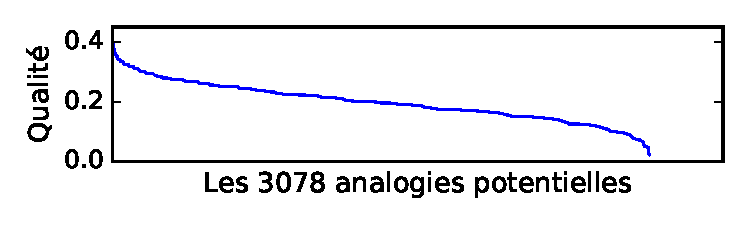
\includegraphics[width=4in]{figures/quality_of_proportions.pdf}
  \caption{Quality of the 993 proportions. The quality of a
  proportion is defined as the fraction of component-proportions that stand
  perfectly.}
\label{FIG:quality_proportions}
\end{figure}
For the best proportions, a perfect analogy stands on more than 70\% of the
components. This is quite significant as we are measuring this fraction over
more than 200 components. However, we have seen that much of these proportions
are not really interesting as all the common users tend to agree on the popular
movies, and the four movies of a proportion tend to be clustered into the same
genre.

To try to exhibit disagreements in the ratings, we used another quality
function. We assign a truth value of $1$ to an analogy $r_1:r_2::r_3:r_4$ if
and only if the proportion complies with one of the following patterns:
\begin{itemize}
  \item $0:1::0:1$,
  \item $1:0::1:0$,
  \item $0:0::1:1$,
  \item $1:1::0:0$.
\end{itemize}
Simply put, we have forbidden the \textit{agreeing analogies} $0:0::0:0$ and
$1:1::1:1$. Figure \ref{FIG:quality_proportions_different_ab_cd} gives us the
fraction of correct proportions for the 993 potential analogies, using this
custom quality function.
\begin{figure}[!h]
\centering
  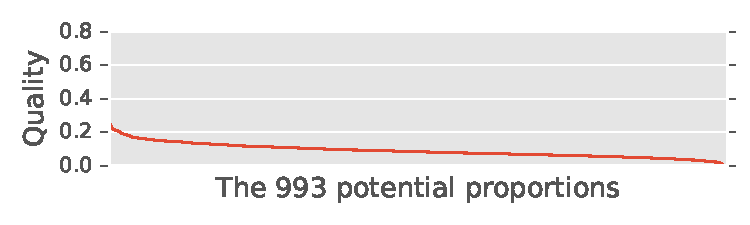
\includegraphics[width=4in]{figures/quality_of_proportions_different.pdf}
  \caption{Quality of the 993 proportions. The quality of a
  proportion is defined as the fraction of components that make up perfect
  proportions, forbidding patterns $0:0::0:0$ and $1:1::1:1$.}
\label{FIG:quality_proportions_different_ab_cd}
\end{figure}
Obviously, the quality drops significantly for the mere reason that we have forbidden patterns
like $r:r::r:r$. This tells us that in fact, \textbf{there are simply not a lot of
interesting analogies}: the best proportion that we found is
\textit{interesting} on less than 25\% of its components, which is quite small.
This confirms our previous observation that sadly, most of the analogies we
find tend to relate four movies that are actual \textbf{neighbors}. We will see
in the conclusion of this chapter how this fact can retrospectively explain the
performances of our basic analogy-based recommender from the first section.

\section*{Conclusion}

In this chapter, we have detailed our contributions to the field of recommender
systems. We have proposed two frameworks based on analogy for the design of
rating prediction algorithms, and also proposed a method for mining analogical
proportions in an incomplete database.

Section \ref{SEC:analogical_reco_basic_algo} described our first attempt at building an analogy-based
prediction algorithm for recommendation. This algorithm is a direct
application of the analogical inference principle, and is strongly related to
the extended classifier that we have described in Chapter
\ref{CHAP:functional_definition}. The basic
underlying idea is that if four users $(a, b, c, d)$ are in analogy regarding their
common items (using the arithmetic proportion), then it should also be the
case for other items that $d$ has not yet rated. We presented a user-based view
where analogies were considered between users, but it is perfectly possible to
consider analogies between items.

We have compared this algorithm with the two main approaches of collaborative
filtering algorithms, namely neighborhood methods and matrix
factorization-based techniques. Our algorithm yields decent accuracy compared
to neighborhood methods, but is extremely expensive in terms of computational resources.
It was clear that this simple and straightforward application of the analogical
inference principle could not be used in real-world settings, where computation
time is a scarce resource.

These observations led us to consider another framework for analogical
recommendation in Section \ref{SEC:clone_based_view}. Acknowledging the fact
that each user tends to have a very
personal idea of what a good (or bad) rating should be, we introduced the notion of clones
which captures how two users tend to agree semantically on a rating. This
semantic agreement is not necessarily reflected in the numerical rating values:
for a user $u$, the value 3 may
be a good rating, while for $v$ it may be a bad one. We derived two algorithms
relying on this clone-based view of the ratings. We also described a quite
recent technique in collaborative filtering, that allows to address user and
item biases. This method is based on the fact that some users tend to give
higher ratings than others, and some items tend to be rated higher than some
other items. We discussed how this view (using biases) is related to our view
(using clones), and pointed out the similarities and differences of the two
approaches. It turned out that these two techniques are really close, and the
resemblance is reflected in the algorithms performances. Yet, as the bias-based
method relies on a global optimization problem, it tends to be better at
capturing the overall noise in the data, and still outperforms our method. Our
last contribution to analogical recommendation was to consider an extreme case
of clone-users, considering that the rating scale $[1, 5]$ could be interpreted
as purely ordinal. Unfortunately, this track of research did not lead to promising results.

In Section \ref{SEC:mining_analogical_proportions}, we proposed an algorithm for the mining of analogical
proportions in a partially described database. This general method perfectly
applies to the problem of mining analogies between users or items in a rating
dataset, such as the one that was used in the first two sections. Based on the
Apriori algorithm, our method is inspired by the mining of association rules
and allows to extract the potential analogies in an efficient way.
We proposed many different quality functions allowing to assess the quality of
a proportion, and naturally some of the quality functions are strongly related
to the Analogical Dissimilarity as defined in Chapter
\ref{CHAP:functional_definition}. We gave
examples of some of the analogies that we found using different variations of
the general mining algorithm, treating ratings as numerical values and as
Boolean values. The main take-away message was that the best analogies that
could be extracted between items were involving users with similar tastes: the four movies of a
proportion were mostly neighbors, in the sense that users tend to agree on
their respective ratings. Also, when forcing proportions to display a
disagreement in the ratings of the four movies, the best proportions that were
revealed still had a pretty bad quality.

This allows us to retrospectively interpret the results of our first
analogy-based prediction algorithm. We have seen that its performances were close to
that of a neighborhood-based technique, but in the light of what has just been
explained we can fairly say that there were no analogies to find in the
database, except for those involving four neighbors. So after all, our
analogy-based inference principle was reduced to that of the classical $k$-NN
approach. Clearly in that case, paying the price of the cubic search in the set
of all users is really not worth it. This is entirely dependent on the database
that was used (in our case, the MovieLens dataset), and we may still presume
that there should exist a dataset where the use of analogical proportion is
beneficial over a simple neighborhood approach.

Even if our investigations on analogical recommendation did not completely live
up to our expectations, there still is a contribution of ours that  is worth
mentioning. As pointed out earlier in the first section, all of our
recommendation experiments
were carried out using Surprise\footnote{\url{http://surpriselib.com}}
\cite{Surprise}, an open source Python recommendation engine that we have
developed. Quite surprisingly, when we started our experiments a few years
ago, there were no Python library that would allow to easily run
cross-validation procedures, or that would make the implementation of a
recommendation algorithm easy. But most importantly, it seemed that most of the
implementation details of the available algorithms were never explicitly
mentioned, so it made comparing performances of the algorithms difficult, if not
meaningless. So we decided to write our own package. We started out by writing
our own custom (and hacky) scripts, which grew up to become a much more
complete and fairly popular recommendation engine. As of April 2017, the main
features of Surprise are the following ones:
\begin{itemize}
  \item Users can have perfect control over their experiments, and to this end
    a strong emphasis was laid on documentation, which we have tried to make as
    clear and precise as possible by pointing out every detail of the
    algorithms.
  \item Dataset handling is made easy. Custom datasets can be used, and the
    MovieLens datasets are natively supported.
  \item Various ready-to-use prediction algorithms are available, such as
    baseline algorithms, neighborhood methods, matrix factorization (SVD,
    PMF, SVD++, NMF), and many others. Also, various similarity measures
    (Cosine, MSD, Pearson \dots) are built-in.
  \item The implementation of new algorithm ideas is made extremely simple.
  \item Cross-validation procedures can be run very easily, as well as
    exhaustive search over a set of parameters for optimization (much like the
    Grid Search feature of the excellent machine learning library scikit-learn
    \cite{scikit-learn}).
\end{itemize}

We now close our discussion on analogical recommendation and on practical
applications of analogy. In the next chapter, we will go back to our original
theoretical considerations, and try to challenge the analogical inference
principle that we have so far blindly followed.


\chapter{Analogy-preserving functions}
\label{CHAP:analogy_preserving_functions}
\localtableofcontents*
\vspace*{\baselineskip}

\initial{W}e first introduced the analogical inference principle in Chapter
\ref{CHAP:formal_analogical_proportions}. This principle states that if four
elements are in analogy, then their classes (or any relevant attribute) should
also be in proportion. This is of course an unsound inference principle, in
that the conclusion does not always follows from the premises. Nonetheless, we
have seen in Chapter \ref{CHAP:functional_definition} that it can still be used
to design some classifiers that we have named conservative and extended
classifiers.  Both in \cite{BayMicDelIJCAI07} and in our experiments in Section
\ref{SEC:experiments_and_empirical_validation}, these classifiers
showed promising results, but were still only used in artificial Boolean
classification problems. Analogical classifiers still had to prove their worth
in real-world applications, and this was precisely the purpose of the last
chapter, where we designed various techniques to apply analogical inference on
a recommendation task.

Unfortunately, the results of a direct application of the analogical inference
principle did not quite live up to our expectations. The conclusion of the last
chapter offered a partial explanation to these modest results, stating that
there were just too few decent analogies to be found on the datasets that we
used. Even if this argument is perfectly admissible, we cannot spare ourselves
the very questioning of the analogical inference principle. We say that if
four elements are in proportion then so are their classes... But why should it
even be true? Actually, this question of \textit{why} will probably be best
answered by philosophers, rather than by computer scientist. We can however
answer the question of \textit{when}: when is the analogical inference
principle sound? Said differently, what are the conditions on the function $f$
so that the inference
$$
\inferrule{\mathbf{a} : \mathbf{b} :: \mathbf{c} : \mathbf{d}}{ f(\mathbf{a}) :
f(\mathbf{b}) :: f(\mathbf{c}) : f(\mathbf{d})}
$$
is sound? The current chapter will be devoted to this question, in a Boolean
setting. In this regard,
the problem we address here is related to the contribution of Davies and Russel
that we described in Section \ref{SEC:Davies_and_Russel} the authors gave a
necessary condition for the following inference principle to hold:
$$\inferrule{P(S) \wedge Q(S) \\ P(T)}{Q(T)}.$$
The links and differences between this inference principle and ours will be
discussed in the conclusion of this document.

It is actually pretty easy to build up simple problems where the application of
our analogical inference principle leads to disastrous results.  Take for
example the problem of Figure \ref{FIG:classif_in_R2}. We have a set $S$ of
points (on the left) that belong to two classes that are linearly separable: an
instance is a square if it is on the left side of the space, else it is a
circle. A naive application of the analogical inference principle would lead us
to believe that for any element that is in proportion with a $3$-tuple in $S^3$
(i.e. the element is the fourth vertex of a parallelogram that we can build
with three elements in $S$), then the classes of the four vertices are in
proportion. In the right figure, we show all these elements, along with their
estimated classes. The result is absolutely terrible, because the whole space
is covered with instances belonging to both of the classes. In this example,
an analogical classifier would lead to ridiculous accuracy results.

\begin{figure}
\centering
\begin{subfigure}{.5\textwidth}
  \centering
  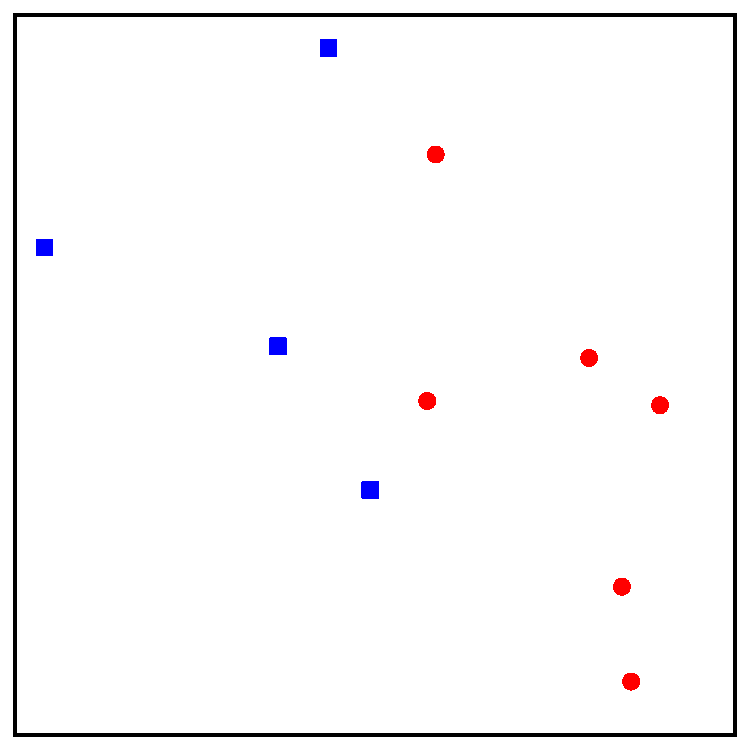
\includegraphics[width=.6\linewidth]{figures/AE_in_R2_S.pdf}
  \label{fig:sub1}
\end{subfigure}%
\begin{subfigure}{.5\textwidth}
  \centering
  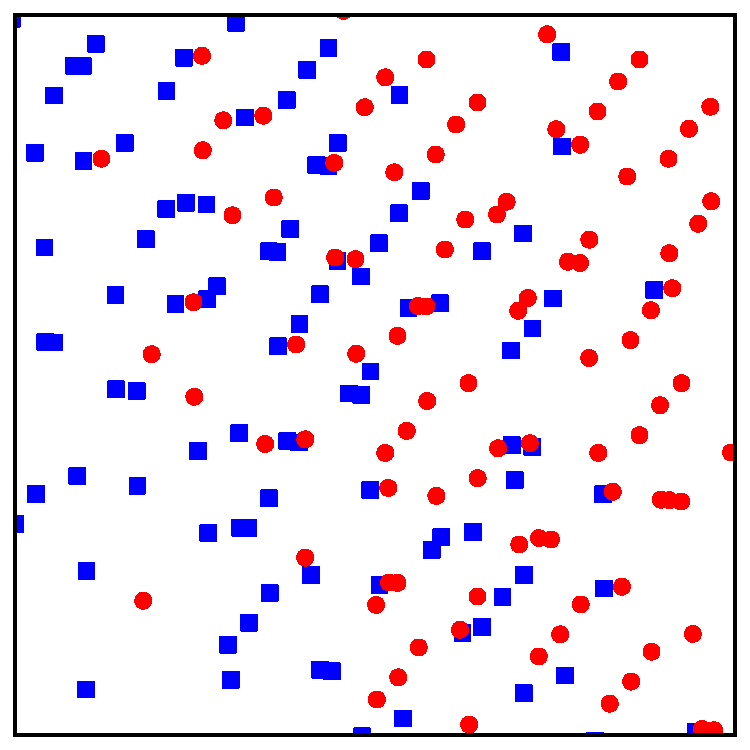
\includegraphics[width=.6\linewidth]{figures/AE_in_R2_AE.pdf}
  \label{fig:sub2}
\end{subfigure}
  \caption{A naive application of the analogical inference principle in
  $\mathbb{R}^2$.}
\label{FIG:classif_in_R2}
\end{figure}

But if it is so easy for our analogical inference principle to fail, then why
does it still work in some cases? Back to Figure \ref{FIG:nan_vs_nn} on page
\pageref{FIG:nan_vs_nn}, the accuracies of the NAN algorithm were definitely
not as bad as that of the problem we have just seen, and some of them were
actually really good. A first obvious difference between the two experiments is
that the one we just described deals with the arithmetic proportion with
real-valued instances, while the other one deals with Boolean attributes. Does
it mean that the analogical inference principle is bound to fail with the
arithmetic proportion? We will probably not be able to completely answer this
question, even though we will provide some insights.  We will instead focus on
the Boolean setting which has seemed to be the most promising for analogical
inference so far, and from there we will derive some links with the real-valued
case.

In this chapter, we will provide a complete characterization of functions that
are fully compatible with the analogical inference principle in a Boolean
setting. Let us restate the inference principle in this context to explain what
we mean: for any four elements $\mathbf{a}, \mathbf{b}, \mathbf{c}, \mathbf{d}$
in $\mathbb{B}^m$, the analogical inference principle states that if
$\mathbf{a}: \mathbf{b}:: \mathbf{c}: \mathbf{d}$, then $f(\mathbf{a}):
f(\mathbf{b}):: f(\mathbf{c}): f(\mathbf{d})$ where $f$ is a Boolean function
from $\mathbb{B}^m$ to $\mathbb{B}$. We have said it before:  this principle is
unsound. The goal of this chapter is to identify all of the functions $f$ that
lead to a valid conclusion, i.e. the functions such that $\mathbf{a}:
\mathbf{b}:: \mathbf{c}: \mathbf{d} \implies f(\mathbf{a}):f(\mathbf{b})::
f(\mathbf{c}): f(\mathbf{d})$ (with some minimal and natural requirements). We
will say that these functions are \textbf{analogy preserving}.

We will tackle this problem by adopting the general point of view of  the
training set extension. In Section \ref{SEC:extending_a_training_set}, we first
define the problem of training set extension, describe some previous works and
explain how this problem can motivate the research of analogy preserving
functions. In Section \ref{SEC:a_complete_characterization_of_AP_functions}, we
give a complete and accurate depiction of analogy preserving functions by
showing that the class of analogy preserving functions is the class of
(Boolean) affine functions. This strong theoretical result is complemented in
Section \ref{SEC:beyond_boolean_AP_functions}, study the some functions that
derive from AP in various ways. We also address the identification of AP
functions in a nominally valued setting and in a real setting, where we will
once again witness the close links between the Boolean proportion and the
arithmetic proportion.

\section{Extending a training set}
\label{SEC:extending_a_training_set}

We have proved in Chapter \ref{CHAP:functional_definition} that the analogical
classification process can be formalized via two new conceptual steps:
\begin{enumerate}
  \item First, the analogical extension $\esf$ of the training set is computed. This
    extension is the set of all elements in the instance space that are in
    analogy with one $3$-tuple in the training set, provided that the
    associated class equation is solvable. Each element of the extension is
    associated with an estimated label: the analogical label denoted $\albl{x}$.
  \item Then, a $k$-NN algorithm is run, considering that the training set is
    now the analogical extension. This $k$-NN classifier allows to
    classify all the elements of the universe that are not in the analogical
    extension.
\end{enumerate}

But then a natural question arises: why should we stick to a $k$-NN classifier?
The reason why the $k$-NN algorithm is used is because in their algorithmic
description, extended learners rely on an analogical dissimilarity, which is
strongly related to a distance on the instance space. But now that we have an
equivalent definition of extended classifiers that does not rely explicitly on
an analogical dissimilarity, nothing actually prevents us from using any other
classifier such as a decision tree, a support vector machine, or any of the
dozens of learners available out there. This would lead us to a different
paradigm for analogical learning: you first extend the training set by building
the analogical extension, and then you are free to do how you please and use
this extension as a bigger training set with any classifier.

In the next subsection, we will formally describe the problem of training set
extension, and present some previous works one this subject. Then in subsection
\ref{SEC:analogy_preserving_presentation}, we will introduce the class of
analogy preserving functions, which lead to a perfectly sound training set
extension in all cases.

\subsection{Previous works on training set extension}

Machine learning algorithms usually require training on sufficiently large
datasets. The problem of learning from few examples is not new and is
referred-to as one-shot learning, where we rely on a transfer of knowledge from
known classes to unknown classes: see  for example \cite{LiFerPerPAMI06} in a
pattern recognition context.  But other options are available when the number
of training instances is small, and training set extension naturally comes in
as a handy tool. Indeed, the extension of the training set is a simple idea to
improve the generalization power of the learner.  The more examples you have, the
better you learn! The point is here to add to the training set $S$ some new
examples, and to try do that in a way that preserves the \textit{quality} of
$S$.

Formally, we start with a set $S= \{\mathbf{x}^{(i)} \in X^m| i \in
[1,n]\}$ of examples ($n$ is supposed to be small), where $\mathbf{x}^{(i)}$ is
an element of a Cartesian product $X^m = X_1 \times \ldots \times X_m$.
For each element  $\mathbf{x}^{(i)} \in S$, we associate a target
$f(\mathbf{x}^{(i)})=y^{(i)} \in Y$.  In the case of regression, $y^{(i)} \in
\mathbb{R}$, and in the case of classification $y^{(i)}$ belongs to a finite
set.

Actually, only a few methods have been proposed for extending a training set with
new examples, and most of them are specific to a particular application. For
example in \cite{CanPerArlLlo06}, some techniques are proposed but they are
only relevant for character recognition tasks. Intuitively, we may build a new
example starting from 1, 2 or 3 known examples.
\begin{enumerate}
\item With one example, a natural way to proceed is to use the classical
  neighborhood approach: given one  example $(\mathbf{a},f(\mathbf{a}))$, we
    can generate a new example $(\mathbf{b},f(\mathbf{b}))$ where  $\mathbf{b}$
    is not too far from $\mathbf{a}$ and $f(\mathbf{b})$ is not too far from
    $f(\mathbf{a})$. In the classification case, $f(\mathbf{b})$ may be chosen
    as $f(\mathbf{a})$. This is the setting in which \cite{CanPerArlLlo06}
    operates, where new characters are generated by slanting, shrinking, and
    dilation of training instances.
\item With two examples, the previous neighborhood option is still available
  and leads to interpolate the new example from the two given ones.  A somehow
    different option is the Feature Knockout procedure \cite{WolMar04}, which
    amounts to build a third example obtained by modifying a randomly chosen
    feature of the first example with that of the second one.  This way to
    proceed enjoys nice properties and appears to be equivalent to the popular
    Tikhonov regularization  technique in the case of linear regression (also
    known  as Ridge regression).  A
    related idea is used in a recent proposal \cite{BouPraRicECAI16} which
    introduces a measure of oddness with regard to a class that is computed on the
    basis of pairs made of two nearest neighbors in the same class; this is
    equivalent to replace the two neighbors by a fictitious representative of
    the class.

\item With three examples $(\mathbf{a},f(\mathbf{a})),
  (\mathbf{b},f(\mathbf{b})), (\mathbf{c},f(\mathbf{c}))$, the previous options
    remain available and lead to build a fourth example which is somehow
    in-between the three other ones: we still have some kind of interpolation.
    A quite different idea is to extrapolate the fourth item on the basis of
    analogical proportions.  In this perspective, this fourth element is not
    necessarily in the neighborhood of the three others. In fact, this idea has
    been addressed in \cite{BayMouMicAnqECML07}, where the authors generated
    new examples that had the least analogical dissimilarity with some
    $3$-tuples in $S^3$. The analogical dissimilarity was an AD between
    sequences, and they used it to generate new examples of handwritten
    characters modeled using the Freeman coding, which is a sequence of symbols
    indicating the successive directions of the pen that are needed to write
    the character. They used their extended training set to train an SVM and a
    Radial Basis Function Network for a classification task, and results showed
    that the classifiers had better results when they were trained with the
    analogically-extended training set than when they were trained with an
    extended training set using other generation techniques (such as those of
    \cite{CanPerArlLlo06}).  Note though that just like the algorithmic
    description of the extended classifier using analogical dissimilarity, we
    here only have an algorithmic description of this training set extension
    procedure. The authors in \cite{BayMouMicAnqECML07} never explicitly refer
    to the analogical extension set $\esf$, and this is normal because the
    unifying framework between the works in \cite{BayMicDelIJCAI07} and the
    works in \cite{StrYvoCNLL05} where only made later in
    \cite{HugPraRicSerECAI16}, as described in Chapter
    \ref{CHAP:functional_definition}.
\end{enumerate}


As far as we know, the problem of generation of new examples has never been
addressed from a theoretical point of view (except for the Knockout procedure,
which is only relevant in some particular settings), and this is actually quite
understandable. Before they can be used in an extended training set, the new
generated examples have to be assigned an estimated label... But how do we
estimate these labels? Well there is a name for such problems: it is called
classification, and classification was the actual reason why we wanted to
extend the training set in the first place, so we have a vicious circle here.
In some sense, extending a training set with potentially noisy data
amounts to nothing but performing classification on a specific set of
instances.

However, training set extension can still be extremely useful if we are
perfectly sure that the new added examples are sound, i.e. that their estimated
labels are the correct ones. In the next subsection, we will formally define
this problem in the context of analogical learning. Section
\ref{SEC:a_complete_characterization_of_AP_functions} will then be devoted to
the identification of the cases where such a perfect extension is feasible.

\subsection {Analogy preserving functions: a safe way to extend a training set}
\label{SEC:analogy_preserving_presentation}

In the rest of this chapter, we will address the problem of extending a
training set using analogical proportions in a Boolean setting. Instead of
using an analogical dissimilarity like in  \cite{BayMouMicAnqECML07}, we will
use our equivalent
functional framework described in Chapter \ref{CHAP:functional_definition},
i.e. we will consider that the extension of the training set $S$ is the
analogical extension $\esf$, where $f$ is the function underlying the ground
truth labels. Algorithmically, the generation of $\esf$ and the computation of
the analogical labels goes as follows:
\begin{enumerate}
  \item Add every $\mathbf{x} \in S$ to $\esf$. Then, for every
    $\mathbf{a},\mathbf{b},\mathbf{c} \in S$ such that $f(\mathbf{a}) :
    f(\mathbf{b}) :: f(\mathbf{c}) : y$ is solvable and such that there is
    $\mathbf{x} \in \mathbb{B}^m \setminus S$ with $\mathbf{a} : \mathbf{b} ::
    \mathbf{c} : \mathbf{x}$, add $\mathbf{x}$ to $\esf$ and save
    the solution $\sol(f(\mathbf{a}), f(\mathbf{b}), f(\mathbf{c}))$ as a candidate
    for $\albl{\mathbf{x}}$.
\item Then for every $\mathbf{x} \in \esfs \eqdef \esf \setminus S$, run a
  \textbf{majority-vote procedure}: set $\albl{\mathbf{x}}$ as the most
    common candidate among all solutions $\sol(f(\mathbf{a}), f(\mathbf{b}),
    f(\mathbf{c}))$ where $(\mathbf{a}, \mathbf{b}, \mathbf{c})$ is in the
    analogical root of $\mathbf{x}$. In case of a tie between two labels, then
    one of the values is chosen at random.  For elements in $S$,
    $\albl{\mathbf{x}}$ is simply set to $f(\mathbf{x})$.
\end{enumerate}

\noindent
The extension $\esf$ is then considered to be an extended training set, where
the labels are the analogical labels, \textbf{which are not necessarily
correct}. Indeed
for some elements $\mathbf{x} \in \esfs$, it may happen that
$\albl{\mathbf{x}} \neq f(\mathbf{x})$, simply because the analogical inference
principle may not be \textit{suitable} for the function $f$. In this chapter,
we  are precisely interested in the identification of all Boolean functions $f$
that lead to perfectly sound extensions, i.e. extensions where the analogical
labels $\albl{\mathbf{x}}$ are always equal to the ground truth values
$f(\mathbf{x})$. These functions will be called \textbf{Analogy preserving}
functions:

\begin{definition}[Analogy preserving functions]
  We say that $\esf$ is {\bf sound} if
  $\albl{\mathbf{x}}=f(\mathbf{x})$ for every $\mathbf{x} \in
  \esfs$. In other words, $\esf$ is sound if $\omegasf
  \eqdef P\left(\albl{\mathbf{x}} = f(\mathbf{x}) \given[\big] \mathbf{x} \in
  \esfs\right) = 1$.

  \noindent
  Also, if $\esf$ is sound for all $S \subseteq
  \mathbb{B}^m$, we say that $f$ is {\bf Analogy Preserving} (AP).
\end{definition}

\noindent
Proposition \ref{PROPOS:equivalent_def_AP} gives an equivalent definition of AP
functions, that will be more useful to convey our proofs:

\begin{proposition}
  \label{PROPOS:equivalent_def_AP}
  A function $f \colon \mathbb{B}^m \to \mathbb{B}$ is AP iff for every
  $\mathbf{a}, \mathbf{b}, \mathbf{c}, \mathbf{d} \in \mathbb{B}^m$, $f$ suits
  the following requirement:
  $$
  \begin{cases}
    \mathbf{a} :  \mathbf{b} ::  \mathbf{c} :  \mathbf{d} \emph{ and }\\
    \emph{solvable}(f(\mathbf{a}), f(\mathbf{b}),  f(\mathbf{c}))
  \end{cases}
  \implies \emph{sol}\left(f(\mathbf{a}),  f(\mathbf{b}),  f(\mathbf{c})\right) =
  f(\mathbf{d}). $$
\end{proposition}
\begin{proof}
  If $f$ fulfills  this requirement, then it is clear from the algorithmic
  description given above that for any $S \subseteq \mathbb{B}^m$ and
  $\mathbf{x} \in \esfs$, all the candidates for $\albl{\mathbf{x}}$ are equal
  to $f(\mathbf{x})$, so $\albl{\mathbf{x}}$ will be invariably set to
  $f(\mathbf{x})$ by the majority-vote procedure, which makes $f$ AP.

If $f$ does not suit this requirement, then there exist $\mathbf{a},
  \mathbf{b}, \mathbf{c}$, and $\mathbf{d} \in \mathbb{B}^m$ such that
  $\mathbf{a} : \mathbf{b} :: \mathbf{c} : \mathbf{d}$ but the solution
  $\sol(f(\mathbf{a}), f(\mathbf{b}), f(\mathbf{c}))$ is not equal to
  $f(\mathbf{d})$. Taking $S_0 = \{\mathbf{a}, \mathbf{b}, \mathbf{c}\}$ we
  obtain $\mathbf{E}^{f*}_{S_0} = \{\mathbf{d}\}$, and since $\albl{\mathbf{d}}
  = \sol(f(\mathbf{a}), f(\mathbf{b}), f(\mathbf{c})) \neq f(\mathbf{d})$, then
  $\mathbf{E}_{S_0}^f$ is not sound so $f$ is not AP.
\end{proof}

\noindent
It should be clear from Proposition \ref{PROPOS:equivalent_def_AP} that looking
for the functions that lead to a perfect extension (i.e. the AP functions) is
equivalent to looking for the functions that are compatible with the analogical
inference principle, which was the first purpose of this chapter. Indeed,
saying that $\sol\left(f(\mathbf{a}),  f(\mathbf{b}),
f(\mathbf{c})\right) =f(\mathbf{d})$ is equivalent to saying that
$f(\mathbf{a}) : f(\mathbf{b}) ::  f(\mathbf{c}) :  f(\mathbf{d})$.

Let us note that many natural functions are not AP. Consider for example the
binary function $f(x_1,x_2)= x_1 \wedge x_2$, along with $\mathbf{a},
\mathbf{b}, \mathbf{c}, \mathbf{d} \in \mathbb{B}^2$ in Table
\ref{exampleNotAP}.  We have $\mathbf{a} : \mathbf{b} :: \mathbf{c} :
\mathbf{d}$ and $f(\mathbf{a}) : f(\mathbf{b}) :: f(\mathbf{c}) : y$ is
solvable, yet the solution is $\sol(f(\mathbf{a}), f(\mathbf{b}),
f(\mathbf{c}))=0$, which  is different from $f(\mathbf{d})=1$ so $f$ is not AP.
This actually comes from the fact that analogical proportions are not stable by
conjunction combination. It is also the case for the disjunction
\cite{PraRic14}.

\begin{table}[ht]
  \center
$\begin{array}{cccc}
  \toprule
  ~ & x_1 & x_2 & f(\cdot) \\
  \midrule
  \mathbf{a} & 0 & 0 & 0\\
  \mathbf{b} & 0 & 1 & 0\\
  \mathbf{c} & 1 & 0 & 0\\
  \mathbf{d} & 1 & 1 & 1\\
  \bottomrule
\end{array}
$\bigskip
\caption{$f(x_1,x_2)= x_1 \wedge x_2$ is not AP.}
\label{exampleNotAP}
\end{table}

The following section will be devoted to a complete characterization of AP
functions in a Boolean setting.

\section{A complete characterization of analogy preserving functions}
\label{SEC:a_complete_characterization_of_AP_functions}

We will show in this section that the class of AP functions is the class of
affine functions, which will be defined later. To complete our proofs, we will
first need to recall some background knowledge on Boolean algebra and Boolean
functions, which is the purpose of the next subsection.

\subsection{Preliminary background on Boolean functions}

Our first step will be to use a unifying notation for all of the Boolean
functions, and to adopt an algebraic point of view.  In the following, the AND
operator `$\wedge$' will be denoted `$\cdot$', and `$+$' will now denote the
modulo-2 addition, equivalent to the XOR operator.  We shall make use of the
polynomial representation of Boolean functions, that we now describe. A
\textbf{ monomial} is a term of the form:
$$\mathbf{x}_I=\underset{i\in I}{\prod}x_i,$$ for some possibly empty finite
set of positive integers $I$, where $|I|$ is called the \textbf{degree} of
$\mathbf{x}_I$. Simply put, a monomial is a conjunction of variables. We take
the convention that $1$ is the empty monomial $\mathbf{x}_\emptyset $. A
\textbf{ polynomial} is a sum of monomials and its degree is the largest degree
of its monomials.  It is well-known \cite{StoneAlgebra36,ZhegalkinAlgebra27}
that \textbf{any function $f:\mathbb{B}^m\rightarrow \mathbb{B}$ is uniquely
represented by a polynomial}, also called the \textbf{Algebraic Normal Form}
(ANF) of $f$:
$$f(x_1,\ldots,x_m)=\sum_{I\subseteq \{1,\ldots,m\}}a_I\cdot \mathbf{x}_I,$$
where each $a_I$ belongs to $\mathbb{B}$. Note that the
constant function $0$ is represented by $a_\emptyset\cdot \mathbf{x}_\emptyset$
with $a_\emptyset =0$. The degree of a function $f:\mathbb{B}^m\rightarrow
\mathbb{B}$, denoted $d(f)$, is defined as the degree of the unique polynomial
representing $f$. In the following, we will often will refer to $f$ as both a
function object and as the associated ANF.

\begin{testexample}
To illustrate this concept, here are
the ANF of some common Boolean functions in $\mathbb{B}^2$ or $\mathbb{B}$:

\begin{itemize}
  \item $\text{AND}(x_1, x_2) = x_1 \cdot x_2$ ;
  \item $\text{OR}(x_1, x_2) = x_1 + x_2 + x_1 \cdot x_2$ ;
  \item $\text{XOR}(x_1, x_2) = x_1 + x_2$ ;
  \item $\text{NEG}(x_1) = x_1 + 1$.
\end{itemize}
\end{testexample}

Another key concept of our proof is the notion of essential and inessential
variables.  For $k\in [1,m]$, $\boldsymbol{\alpha}\in \mathbb{B}^m$, and $c \in
\mathbb{B}$, let ${\boldsymbol{\alpha}}_{k}^c$ be the tuple in $\mathbb{B}^{m}$
whose $i$-th component is set to $c$ if $i=k$, and to $\alpha_i$ otherwise.  A
variable $x_i$ is said to be \textbf{inessential} in $f\colon \mathbb{B}^m\to
\mathbb{B}$ if for all $\boldsymbol{\alpha} \in \mathbb{B}^m$ and $c \in
\mathbb{B}$, $f(\boldsymbol{\alpha}^c_i) = f(\boldsymbol{\alpha}^{\neg c}_i)$.
Otherwise, $x_i$ is said to be \textbf{essential} in $f$, or that $f$ depends
on $x_i$. In simple terms, an essential variable is a variable that has the
\textit{ability} to change the value of $f$. In fact, it can be shown that if
$x_i$ is an inessential variable for a function $f$, then $x_i$ does not appear
in the ANF of $f$.  For example in $f(x_1, x_2, x_3) = x_1 \cdot x_3$, $x_1$
and $x_3$ are essential variables while $x_2$ is inessential.  We denote by
$\ess(f)$ the number of essential variables of $f$ (or \textbf{essential
arity}).

Two functions $f\colon \mathbb{B}^m\to \mathbb{B}$ and $g\colon \mathbb{B}^n\to
\mathbb{B}$ are said to be {\bf equivalent} if there exist two mappings
$\sigma\colon
[1,n]\to [1,m]$ and $\sigma'\colon [1,m]\to [1,n]$ such that
\begin{align*}
  f(x_1,\ldots , x_m)&=g(x_{\sigma(1)},\ldots,x_{\sigma(n)}) \text{ and} \\
   g(x_1,\ldots , x_n)&=f(x_{\sigma'(1)},\ldots,x_{\sigma'(m)}).
\end{align*}
In other words, $f$ and $g$ are equivalent if one can be obtained from the
other by permutation of variables, addition of inessential variables, or
identification of inessential variables. Another point of view is to consider
that two functions are equivalent if their ANF is the same, up to the
renaming of variables. For example, $f(x_1, x_2, x_3) = x_1
\cdot x_3$ and $g(x_1, x_2)  = x_1 \cdot x_2$ are equivalent functions. Note
that two equivalent functions necessarily have the same number of essential
variables. For further background in the theory of essential variables of
functions, see \cite{CouceiroTCS08, CouceiroDM09, SalomaaAASF63, WillardDM96}.
In our demonstrations, we will use the following property:

\begin{property}\label{equivalent_functions}
Let $f\colon \mathbb{B}^m\to \mathbb{B}$ and $g\colon \mathbb{B}^n\to
  \mathbb{B}$ be equivalent functions. Then $f$ is AP if and only if $g$ is AP.
\end{property}

This can be verified by noting that as the analogy in $\mathbb{B}^m$ is defined
in a component-wise fashion, the permutation of variables has no effect on the equation and
its solution. Also, manipulation of inessential variables do not change the
value of the function $f$, and thus the AP property still holds.

We now define the concept of \textbf{section} of a function, also known as a
\textit{restriction}, or equivalently as the result of \textit{partial
application} in computer science. Let $f$ be a function $\mathbb{B}^m\to
\mathbb{B}$, and $(I, J)$ be a partition of $[1, m]$. With $\mathbf{x} \in
\mathbb{B}^m$ and $\boldsymbol{\alpha} \in \mathbb{B}^{|I|}$, the $I$-section
(or simply section) $f^{\boldsymbol{\alpha}}_I \colon \mathbb{B}^{|J|} \to
\mathbb{B}$ is the function that is obtained after setting all variables in $I$
to the components of $\boldsymbol{\alpha}$.  More formally, let us define
$(\mathbf{x}^{\boldsymbol{\alpha}}_I) \in \mathbb{B}^m$ as follows:
$$
\begin{cases}
(\mathbf{x}^{\boldsymbol{\alpha}}_I)_i \eqdef x_i \mbox{ if } i \notin I\\
(\mathbf{x}^{\boldsymbol{\alpha}}_I)_i \eqdef \alpha_j \mbox{ where } j \mbox{
  is the index of } i \mbox{ in } I.
\end{cases}
$$
Concretely, Concretely, $\mathbf{x}^{\boldsymbol{\alpha}}_I$ is nothing but the vector $\mathbf{x}$
where the components at the  indices in $I$ have been replaced by the
successive components of $\boldsymbol{\alpha}$. For instance, with $m=5,
\mathbf{x}=(0,1,1,0,0), I=\{1,3,4\}$ and $\boldsymbol{\alpha}=(1,0,0)$, we
have $(\mathbf{x}^{\boldsymbol{\alpha}}_I)=(1,1,0,0,0)$.  The $I$-section
$f^{\boldsymbol{\alpha}}_I$ is the function from $\mathbb{B}^{\mid J \mid} \to
\mathbb{B}$ defined as:
$$\forall \mathbf{y} \in \mathbb{B}^{|J|},~~
f^{\boldsymbol{\alpha}}_I(\mathbf{y}) \eqdef
f((\mathbf{x}^{\boldsymbol{\alpha}}_I)^\mathbf{y}_J).$$
Note that the arity of $f^{\boldsymbol{\alpha}}_I$ is $|J|$ and is always less
than the arity of $f$, and that
$\ess(f^{\boldsymbol{\alpha}}_I) \leq \ess(f)$.  As an example, let us consider
the function $f\colon \mathbb{B}^3 \to \mathbb{B}$ such as
$$f(x_1,x_2, x_3) = x_1 \cdot x_2 \cdot x_3 + x_1 \cdot x_2 + x_3.$$
The section $f^{(1, 0)}_{\{1, 3\}}$ is a function from $\mathbb{B}$ to
$\mathbb{B}$ and is defined by $f^{(1, 0)}_{\{1, 3\}}(x_2) = x_2$.
A main result about sections that will be used in other proofs is stated in
Property \ref{section_preserve_wap}:

\begin{property}\label{section_preserve_wap}
If $f\colon \mathbb{B}^m\to \mathbb{B}$ is AP, then every section of $f$ is
  also AP.
\end{property}
\begin{proof}
  This statement is actually pretty obvious but sadly, its proof is quite ugly.
  Let $f$ be an AP function from $\mathbb{B}^m \to \mathbb{B}$, $(I,J)$ a
  partition of $[1, m]$, and $\boldsymbol{\alpha} \in \mathbb{B}^{|I|}$. We
  will consider the section  $f^{\boldsymbol{\alpha}}_I$.  Let's now assume
  that we have $\mathbf{a},\mathbf{b},\mathbf{c}, \mathbf{d} \in
  \mathbb{B}^{|J|}$ with the 2 following properties:
  $$
  \begin{cases}
    \mathbf{a}:\mathbf{b}::\mathbf{c}:\mathbf{d}\\
    \solvable(f^{\boldsymbol{\alpha}}_I(\mathbf{a}),
    f^{\boldsymbol{\alpha}}_I(\mathbf{b}),
    f^{\boldsymbol{\alpha}}_I(\mathbf{c}))
  \end{cases}
  $$
  We want to prove that this implies that
  $\sol(f^{\boldsymbol{\alpha}}_I(\mathbf{a}),
  f^{\boldsymbol{\alpha}}_I(\mathbf{b}), 
  f^{\boldsymbol{\alpha}}_I(\mathbf{c}))
  =
  f^{\boldsymbol{\alpha}}_I(\mathbf{d})$.
  First, let us note that the following property holds:
$$\forall \mathbf{a},\mathbf{b},\mathbf{c}, \mathbf{d} \in \mathbb{B}^{|J|},~J
  \subset [1,m], ~ \mathbf{x} \in \mathbb{B}^m,~~ \mathbf{a}: \mathbf{b} ::
  \mathbf{c} : \mathbf{d} \implies \mathbf{x}^{\mathbf{a}}_J :
  \mathbf{x}^{\mathbf{b}}_J:: \mathbf{x}^{\mathbf{c}}_J :
  \mathbf{x}^{\mathbf{d}}_J,$$
  simply due to the fact that $\mathbf{x}:\mathbf{x}::\mathbf{x}:\mathbf{x}$
  always holds.

Regarding the first condition $\mathbf{a}:\mathbf{b}::\mathbf{c}:\mathbf{d}$,
since $\forall \mathbf{x} \in \mathbb{B}^m,$ we have that $
  \mathbf{x}^{\boldsymbol{\alpha}}_I : \mathbf{x}^{\boldsymbol{\alpha}}_I ::
  \mathbf{x}^{\boldsymbol{\alpha}}_I : \mathbf{x}^{\boldsymbol{\alpha}}_I$, we
  deduce: $(\mathbf{x}^{\boldsymbol{\alpha}}_I)^{\mathbf{a}}_J :
  (\mathbf{x}^{\boldsymbol{\alpha}}_I)^{\mathbf{b}}_J ::
  (\mathbf{x}^{\boldsymbol{\alpha}}_I)^{\mathbf{c}}_J :
  (\mathbf{x}^{\boldsymbol{\alpha}}_I)^{\mathbf{d}}_J$.
By definition $f^{\boldsymbol{\boldsymbol{\alpha}}}_I(\mathbf{y}) =
  f((\mathbf{x}^{\boldsymbol{\alpha}}_I)^{\mathbf{y}}_J)$, and the second
  condition is just:
  $$\solvable(f((\mathbf{x}^{\boldsymbol{\alpha}}_I)^\mathbf{a}_J),
  f((\mathbf{x}^{\boldsymbol{\alpha}}_I)^\mathbf{b}_J),
  f((\mathbf{x}^{\boldsymbol{\alpha}}_I)^\mathbf{c}_J)).$$
  Since $f$ is AP, we have that
  $\sol(f((\mathbf{x}^{\boldsymbol{\alpha}}_I)^\mathbf{a}_J),
  f((\mathbf{x}^{\boldsymbol{\alpha}}_I)^\mathbf{b}_J),
  f((\mathbf{x}^{\boldsymbol{\alpha}}_I)^\mathbf{c}_J))=
  f((\mathbf{x}^{\boldsymbol{\alpha}}_I)^\mathbf{d}_J) \eqdef
  f^{\boldsymbol{\alpha}}_I(\mathbf{d})$,
  which is precisely the condition for
  $f^{\boldsymbol{\boldsymbol{\alpha}}}_I$ to be AP.
\end{proof}


This section was quite dense so let us recap what we have seen. We
describe functions by their ANF, which is a polynomial representation. This ANF
allowed us to define the degree of a function, which has a similar meaning to
the notion of degree for real valued polynomials. We also defined the notion of
equivalent functions, and showed that two equivalent functions are either both
AP, or none of them are. Finally, we defined the section of a function which is
a function of lower arity, and saw that sectioning an AP function leads to
another AP function.

We are now in a position to see some examples of AP functions. We will first
show that any affine function is AP, and we will then prove that these
functions are actually the only AP functions.

\subsection{The class of Analogy Preserving functions}
\label{SEC:the_class_of_AP_functions}

Let us first define the class of affine functions:
\begin{definition}[Affine functions]
  The class $L$ of \textbf{affine} functions is the set of functions $f$ of the
  form:
  $$f(x_1,\ldots , x_m)=\alpha_1\cdot x_1+\ldots +\alpha_m\cdot
  x_m+\alpha_0,$$
  where $\alpha_0,\ldots, \alpha_m$ are elements of $\mathbb{B}$. We also write
  $$f(\mathbf{x}) = \boldsymbol{\alpha} \cdot \mathbf{x} + \alpha_0,$$
  where $\boldsymbol{\alpha} \in \mathbb{B}^m$ and $\cdot$ is here a scalar
  product.  If $\alpha_0= 0$ we say that $f$ is \textbf{linear}.
\end{definition}

Note that we used the polynomial representation of the function $f$, and that
$L$ is precisely the set of functions whose degree is less than or equal to
$1$. Informally, a linear function is a function that computes the exclusive OR
between any subset of variables. The class $L$ of affine functions is then the set of all linear
functions along with their negations (because $f + 1$ = $\neg f$). A particular
case of affine functions are the \textbf{projections} or \textbf{dictator}
functions, defined by $f(\mathbf{x}) = x_i + \alpha_0$. These functions will be
of interest in the next subsection.

Now, we will prove that every affine function is AP:
\begin{proposition}
  \label{PROPOS:affine_functions_are_ap}
  Any affine function $f$ is AP.
\end{proposition}

\begin{proof}
  Let $f \colon \mathbb{B}^m \to \mathbb{B} \in L$. Using the obvious fact that
  $f$ is AP  iff $f + 1 = \neg f$ is AP, we may assume without loss of
  generality that $\alpha = 0$. Also, considering that $f$ essentially depends
  on $n \leq m$ variables ($n$ is then the number of $\alpha_i$ equal to $1$),
  $f$ is equivalent to the function $g \colon \mathbb{B}^n \to \mathbb{B}$
  defined by $g(x_1, \cdots, x_n) = x_1 +  \cdots + x_n$. Using Property
  \ref{equivalent_functions}, we just need to prove that $g$ is AP to show that
  $f$ is also AP.

  This function $g$ has the remarkable property\footnote{This is the reason why
  affine functions lead to classification problems that are, in fact, highly
  \textbf{non} linearly separable.} that changing the value of any $x_i$
  changes the value of $g$: $\forall _i, \quad g(x_1, \cdots, x_i, \cdots, x_n)
  = \neg g(x_1, \cdots, \neg x_i, \cdots, x_n)$, as illustrated on Figure
  \ref{FIG:affine_functions_neighbors}. From this property, it is easy to see
  that:
  $$\forall \mathbf{x}, \mathbf{x}' \in \mathbb{B}^n, g(\mathbf{x}) =
  g(\mathbf{x}') \iff H(\mathbf{x}, \mathbf{x}') \text{ is even},$$
  where $H$ is the Hamming distance function.

  Let $\mathbf{a}, \mathbf{b}, \mathbf{c}, \mathbf{d} \in \mathbb{B}^n$  such
  that the two hypothesis in the definition of AP are satisfied, i.e.
  $$
  \mathbf{a} : \mathbf{b} :: \mathbf{c} : \mathbf{d}\quad \text{and}\quad
  g(\mathbf{a}) : g(\mathbf{b}) :: g(\mathbf{c}) : y\quad  \text{is  solvable}.
  $$

  This equation is solvable in two possible cases: either $g(\mathbf{a}) =
  g(\mathbf{b})$, or $g(\mathbf{a}) = g(\mathbf{c})$. This can be verified in
  Table \ref{TAB:six_valid_patterns} on page \pageref{TAB:six_valid_patterns},
  or by referring to Proposition \ref{PROPOS:equation_solving}.
  Also, we know from Property \ref{PROPER:hamming_distance_boolean_proportion}
  that as $\mathbf{a} : \mathbf{b} :: \mathbf{c} : \mathbf{d}$, we have
  $H(\mathbf{a}, \mathbf{b}) = H(\mathbf{c}, \mathbf{d})$ and $H(\mathbf{a},
  \mathbf{c}) = H(\mathbf{b}, \mathbf{d})$.
  Therefore, we either are in one of the two following cases:
  \begin{enumerate}
    \item $g(\mathbf{a}) = g(\mathbf{b})$, and in this case the solution is
      $\sol(g(\mathbf{a}), g(\mathbf{b}), g(\mathbf{c})) = g(\mathbf{c})$. As
      $g(\mathbf{a}) = g(\mathbf{b})$, then $H(\mathbf{a}, \mathbf{b})$ is
      even, and so is $H(\mathbf{c}, \mathbf{d})$. Then, $g(\mathbf{c}) =
      g(\mathbf{d})$, and thus $\sol(g(\mathbf{a}), g(\mathbf{b}),
      g(\mathbf{c})) = g(\mathbf{d})$.
    \item $g(\mathbf{a}) = g(\mathbf{c})$, and in this case the solution is
      $\sol(g(\mathbf{a}), g(\mathbf{b}), g(\mathbf{c})) = g(\mathbf{b})$. As
      $g(\mathbf{a}) = g(\mathbf{c})$, then $H(\mathbf{a}, \mathbf{c})$ is
      even, and so is $H(\mathbf{b}, \mathbf{d})$. Then $g(\mathbf{b}) =
      g(\mathbf{d})$, and thus $\sol(g(\mathbf{a}), g(\mathbf{b}),
      g(\mathbf{c})) = g(\mathbf{d})$.
  \end{enumerate}

  In both cases we have $\sol(g(\mathbf{a}), g(\mathbf{b}), g(\mathbf{c})) =
  g(\mathbf{d})$, thus showing that $g$ is AP.
  As $g$ and $f$ are equivalent functions, then any function $f \in L$ is AP.
\end{proof}

\begin{figure}[!h]
\centering
  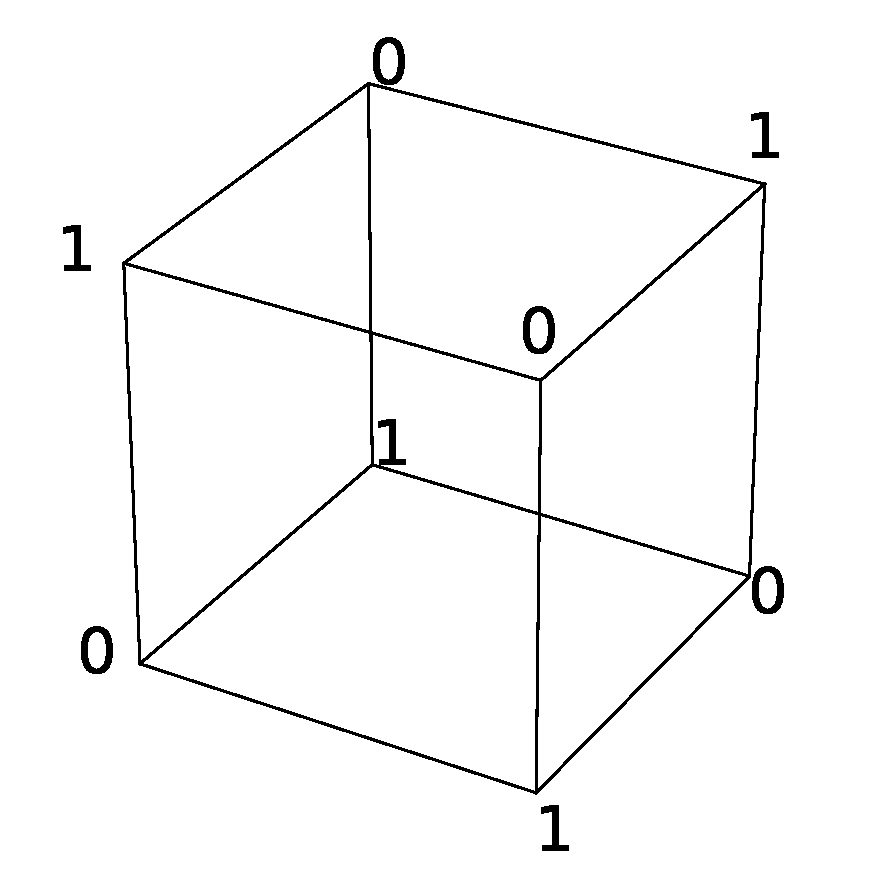
\includegraphics[width=2in]{figures/affine_functions_neighbors.pdf}
  \caption{The labels as determined by the affine function $g(x_1, x_2, x_3) =
  x_1 + x_3 + x_3$. Note that each $1$ is surrounded by three $0$, and each $0$
  is surrounded by three $1$. Also, note that solving any (solvable) analogical
  equation leads to the correct solution: This is because $g$ is AP.}
  \label{FIG:affine_functions_neighbors}
\end{figure}

Proposition \ref{PROPOS:affine_functions_are_ap} can now retrospectively
explain the results of Figure \ref{FIG:nan_vs_nn} on page \ref{FIG:nan_vs_nn}
for the two functions $f_1$ and $f_2$, which are both instances of affine
functions. We saw that for these two functions, $\omegasf$ (defined as the
proportion of elements $\mathbf{x}$ in $\esfs$ for which $\albl{x} = f(x)$) was
always equal to $1$. This result is now obvious and directly comes from the
fact that both $f_1$ and $f_2$ are actually analogy preserving functions: $f_1$
was a projection function while $f_2$ was a general affine function.

We now know that every affine function is AP. We will here give a stronger
result: the affine functions are the \textbf{only} AP functions.  In the
previous subsection, we introduced the ANF of Boolean functions and also
defined their degree. We also mentioned that the class of functions with degree
at most $1$ is exactly the class $L$ of affine functions, which are AP.  We
will show that the class of AP functions is the class of affine functions by
proving that if a function $f$ is AP, then $d(f)\leq 1$. Let us first consider
the case where $d(f) = 2$:

\begin{property} \label{degree_2_not_AP}
 Let $f\colon \mathbb{B}^m\to \mathbb{B}$ with $d(f)=2$. $f$ is not AP.
\end{property}
\begin{proof}
  Let's consider $f$ with $d(f) = 2$ and $\ess(f) >= 2$. We denote
  $\mathbf{x}_I$ one of the monomial of $f$ of degree $2$. We consider the
  section $f^{\mathbf{0}}_J$, where $J = [1, m] \setminus I$,  and $\mathbf{0}$
  denotes the constant 0 vector in $B^{|J|}$. All variables that are not part
  of the monomial $\mathbf{x}_I$ have been set to $0$. This section
  $f^{\mathbf{0}}_J$ has a unique monomial of degree $2$ (namely
  $\mathbf{x}_I$) and $\ess(f) = 2$.  $f^{\mathbf{0}}_J$ is necessarily
  equivalent to one of the following functions:
  $$
  \begin{cases}
    f_1(x_1, x_2) = x_1 \cdot x_2 + \alpha_0 \\
    f_2(x_1, x_2) = x_1 \cdot x_2 + x_1 + \alpha_0\\
    f_3(x_1, x_2) = x_1 \cdot x_2 + x_1 + x_2 + \alpha_0
  \end{cases}$$
  To see that none of these functions are AP, consider Table
  \ref{TAB:counter_examples} which gives the values of $f_1, f_2$ and $f_3$
  (with $\alpha_0 = 0$) for the four-tuple $(\mathbf{a}, \mathbf{b},
  \mathbf{c}, \mathbf{d})$.
  \begin{table}[ht]
    \center
  $\begin{array}{cccccc}
    \toprule
    ~ & x_1 & x_2 & f_1 & f_2 & f_3\\
    \midrule
    \mathbf{a} & 0 & 0 & 0 & 0 & 0\\
    \mathbf{b} & 0 & 1 & 0 & 0 & 1\\
    \mathbf{c} & 1 & 0 & 0 & 1 & 1\\
    \mathbf{d} & 1 & 1 & 1 & 0 & 1\\
    \bottomrule
  \end{array}
  $\bigskip
  \caption{Examples for $f_1, f_2, f_3$ showing that they are not AP.}
  \label{TAB:counter_examples}
  \end{table}
  It is clear that the counter-example $(\mathbf{a},\mathbf{b}, \mathbf{c},
  \mathbf{d})$  shows that $f_1$  is not AP because we have $\mathbf{a} :
  \mathbf{b} :: \mathbf{c} : \mathbf{d}$ and the equation $f_1(\mathbf{a}) :
  f_1(\mathbf{b}) :: f(\mathbf{c}) : y$ is solvable, but the solution is $0$
  while $f(\mathbf{d})$ is $1$. Similarly, $(\mathbf{a},\mathbf{b}, \mathbf{c},
  \mathbf{d})$ is also a counter-example for $f_2$ and $(\mathbf{d},\mathbf{c},
  \mathbf{b}, \mathbf{a})$ is a counter-example for $f_3$.

  As $f_1, f_2, f_3$ are not AP, $f^{\mathbf{0}}_J$ cannot be AP either because
  it is equivalent to one of the $f_i$. As $f^{\mathbf{0}}_J$ is a section of
  $f$, $f$ cannot be AP.
\end{proof}

All we need now is a property that could allow us to decrease the degree of a
function without changing the fact that it is AP. This is the purpose of
Property \ref{section_degree_k_minus_1}.

\begin{property}\label{section_degree_k_minus_1}
Let $f:\mathbb{B}^m\rightarrow \mathbb{B}$ be a function with
  $d(f)=k\geq 2$. Then there is a section $g$ of $f$ with $d(g)=k-1$.
\end{property}
\begin{proof}
Suppose that  $d(f)=k\geq 2$, and let $\mathbf{x}_I$ be a monomial of $f$ of
  maximum degree, i.e. $|I|=k$.  Here again, consider the section $g =
  f^{\mathbf{0}}_J$ where $J = [1, m] \setminus I$ and $\mathbf{0}$ denotes the
  constant $0$ vector in $\mathbb{B}^{|J|}$. It is clear that $g$ is
  represented by a  polynomial that has a unique monomial of maximal degree
  $k$, namely $\mathbf{x}_I$, and maybe some other monomials of degree strictly
  less than $k$.  Let us choose any $i \in I$: then $g' = g^1_{\{i\}}$ is a
  section of $g$ of degree (and arity) $k-1$. As $g'$ is a section of $g$, it
  is also a section of $f$ which completes the proof.
\end{proof}

We are now in position to prove our main result.

\begin{proposition}
  \label{PROPOS:AP_is_L}
The class of AP functions is the class $L$ of affine functions.
\end{proposition}
\begin{proof}
We have seen that every affine function is AP, i.e. if $d(f)\leq 1$, then $f\in
  AP$. On the other hand, Property \ref{degree_2_not_AP} tells us that if
  $d(f)=2$, then $f \notin AP$. So suppose that  $d(f)\geq 3$. By successive
  applications of Property \ref{section_degree_k_minus_1}, it follows that
  there is a section $g$ of $f$ with $d(g)=2$.

  As $g$ is not AP, then $f$ is not AP either. All in all, if $d(f) \geq 2$
  then $f$ is not AP, so the class of AP functions is $L$.
\end{proof}

In the end, we proved that {\bf the class of functions that ensure a sound
analogical extension of any training set $S \subseteq \mathbb{B}^m$ is the class
of affine functions $L$}. If the function is not affine, then there exist a
training set $S \subseteq \mathbb{B}^m$ for which $\mathbf{E}_S(f)$ is unsound.
We can now finally give a definite answer to our initial problem: \textbf{a
function $f$ is \textit{compatible} with the analogical inference principle if
and only if $f$ is affine.}

In the next subsection, we will focus on some AP functions that are still
\textit{compatible} with the analogical inference principle, but in a stronger
sense.

\subsection{The class of Strongly Analogy Preserving functions.}
\label{SEC:the_class_of_SAP_functions}

Let us come back to the analogical inference principle for a moment, which
states that if we have  $\mathbf{a}: \mathbf{b}:: \mathbf{c}: \mathbf{d}$, then
we should also have $f(\mathbf{a}) :f(\mathbf{b}) :: f(\mathbf{c}) :
f(\mathbf{d})$:
$$
\inferrule{\mathbf{a} : \mathbf{b} :: \mathbf{c} : \mathbf{d}}{ f(\mathbf{a}) :
f(\mathbf{b}) :: f(\mathbf{c}) : f(\mathbf{d}) }
$$
Something we have overlooked so far but that is of importance, is that
implicitly this inference principle requires that the class equation
$f(\mathbf{a}) : f(\mathbf{b}) :: f(\mathbf{c}) : y$ is solvable as soon as we
have $\mathbf{a} : \mathbf{b} :: \mathbf{c} : \mathbf{d}$. Indeed if the
equation is not solvable, then we simply cannot have $f(\mathbf{a}) :
f(\mathbf{b}) :: f(\mathbf{c}) : f(\mathbf{d})$.
Therefore, a more explicit writing of the analogical inference principle is as
follows:
$$
\inferrule[\text{~~ Inference Principle A}]{\mathbf{a} : \mathbf{b} :: \mathbf{c} :
\mathbf{d}}{\solvable(f(\mathbf{a}), f(\mathbf{b}),
f(\mathbf{c})) \\\\f(\mathbf{a}) : f(\mathbf{b}) :: f(\mathbf{c}) :
f(\mathbf{d}) }
$$


Yet, in the end, the ultimate use of this principle is to infer the value of
$f(\mathbf{d})$, and we can only do that by the actual solving of the equation
$f(\mathbf{a}) : f(\mathbf{b}) :: f(\mathbf{c}) : y$ (remember that when we
build the analogical extension, we always require the class equation to be
solvable). This was also the case when we where dealing with the algorithmic
description of the conservative classifier (see e.g. Algorithm
\ref{ALGO:conservative_classifier}).  So if the equation is not
solvable, we are unable to infer anything about $f(\mathbf{d})$. This is why
the AP functions are defined as the functions such that we have $f(\mathbf{a})
:f(\mathbf{b}) :: f(\mathbf{c}) : f(\mathbf{d})$ provided that
$\mathbf{a}: \mathbf{b}:: \mathbf{c}: \mathbf{d}$ stands \textbf{and that}
$f(\mathbf{a}) :f(\mathbf{b}) :: f(\mathbf{c}) : y$ is solvable. With regard to
this, we can say the class of AP functions are the class of functions that
allow the following inference principle to be sound: $$
\inferrule[\text{~~ Inference principle B}]{\mathbf{a} : \mathbf{b} ::
\mathbf{c} : \mathbf{d} \\\\ \solvable(f(\mathbf{a}), f(\mathbf{b}),
f(\mathbf{c}))}{f(\mathbf{a}) : f(\mathbf{b}) :: f(\mathbf{c}) : f(\mathbf{d})}
$$

\textbf{This one is the inference principle that is actually useful in
practice}: if the
equation is not solvable then we simply try another $4$-tuple. The first one is
too restrictive on the function $f$ because it requires that $\mathbf{a} :
\mathbf{b} :: \mathbf{c} : \mathbf{d} \implies  \solvable(f(\mathbf{a}),
f(\mathbf{b}), f(\mathbf{c}))$, and in practice this requirement is not
needed.

We have shown that the AP functions are those that are lead the inference
principle B to be sound.  For the sake of completeness however, we will also
identify the functions that lead the inference principle A to be sound. These
functions will be called Strongly Analogy Preserving functions (SAP):

\begin{definition}[Strongly analogy preserving functions]
  A function $f$ is Strongly Analogy Preserving (SAP) if:
  $$\forall \mathbf{a}, \mathbf{b}, \mathbf{c}, \mathbf{d} \in \mathbb{B}^m, ~~
  \mathbf{a}: \mathbf{b}:: \mathbf{c}: \mathbf{d} \implies
  \begin{cases}
    \text{solvable}(f(\mathbf{a}), f(\mathbf{b}), f(\mathbf{c}))\\
     f(\mathbf{a}) : f(\mathbf{b}) :: f(\mathbf{c}) : f(\mathbf{d}).
  \end{cases}$$
\end{definition}

We will show that the SAP functions are the dictator functions, i.e. functions
of the form $f(\mathbf{x)} = x_i + \alpha_0$ for some $i \in [1, m]$.
Naturally, these are a subclass of affine functions, because every SAP function
is necessarily AP. In Property \ref{PROPER:projections_are_sap}, we prove that
every dictator function  is SAP.

\begin{property}
  \label{PROPER:projections_are_sap}
  Let $f$ be a dictator function, i.e. an affine function a the form:
  $$f(x_1, x_2, \cdots, x_m) = x_i + \alpha_0,$$
  where $i \in [i, m]$ and $\alpha_0 \in \mathbb{B}$. Then $f$ is SAP.
\end{property}
\begin{proof}
  Let $f$ be a dictator function: $f(\mathbf{x}) = x_i$ (we consider $\alpha_0$
  to be $0$ for now). Consider $\mathbf{a}, \mathbf{b}, \mathbf{c}, \mathbf{d}
  \in \mathbb{B}^m$ such that $\mathbf{a}: \mathbf{b}:: \mathbf{c}:
  \mathbf{d}$.

  As the analogy is defined component-wise, this means that we have in
  particular $a_i : b_i :: c_i : d_i$, which is strictly equivalent to
  $f(\mathbf{a}) : f(\mathbf{b}) :: f(\mathbf{c}) : f(\mathbf{d})$, so $f$ is
  SAP. The case where $\alpha_0 = 1$ is derived in the same obvious way.
\end{proof}

We now show that the dictator functions are the only SAP functions:

\begin{proposition}
  The class of SAP functions is the class of dictator functions.
\end{proposition}
\begin{proof}
  We already know that a SAP function is an AP function, so a SAP function
  necessarily is affine. Consider a function $f$ that is affine but that is not
  a dictator function, i.e. $f$ is of the form:
  $$f(\mathbf{x}) = \alpha_1 \cdot x_1 + \cdots +\alpha_m \cdot x_m + \alpha_0,$$
  with at least $\alpha_i = 1$ and $\alpha_j = 1$ for two indices $i$ and $j$
  with $i\neq j \neq 0$. Without loss of generality, we will assume that
  $\alpha_0 = 0$.
  Consider now the four-tuple $(\mathbf{a}, \mathbf{b}, \mathbf{c},
  \mathbf{d})$ such that:
  \begin{itemize}
    \item $a_k = 0$ for all $k \neq i$ and $k\neq j$ ($a_i = a_j = 1$)
    \item $b_k = 0$ for all $k \neq i$ ($b_i = 1$)
    \item $c_k = 0$ for all $k \neq j$ ($c_j = 1$)
    \item $d_k = 0$ for all $k$
  \end{itemize}

  The four-tuple is summarized in Table \ref{TAB:SAP}, where we clearly see
  that we have $\mathbf{a} : \mathbf{b} :: \mathbf{c} : \mathbf{d}$, but the
  equation $f(\mathbf{a}) : f(\mathbf{b}) :: f(\mathbf{c}) : y$ is not solvable
  so $f$ is not SAP, QED.

\begin{table}[ht]
  \center
$\begin{array}{cccc}
  \toprule
  ~ & x_i & x_j & f(\cdot) \\
  \midrule
  \mathbf{a} & 1 & 1 & 0\\
  \mathbf{b} & 1 & 0 & 1\\
  \mathbf{c} & 0 & 1 & 1\\
  \mathbf{d} & 0 & 0 & 0\\
  \bottomrule
\end{array}
$\bigskip
\caption{$f$ is not SAP because $f(\mathbf{a}) : f(\mathbf{b}) :: f(\mathbf{c})
  : y$ is not solvable (plus, $f(\mathbf{a}) : f(\mathbf{b}) :: f(\mathbf{c}) :
  f(\mathbf{d})$ does not stand).}
\label{TAB:SAP}
\end{table}

\end{proof}

This section was quite dense, so let us recap a bit what we have seen so far.
We have given two different instances of the analogical inference principle:
$$
\inferrule[\text{~~ Inference Principle A}]{\mathbf{a} : \mathbf{b} ::
\mathbf{c} : \mathbf{d}}{\solvable(f(\mathbf{a}), f(\mathbf{b}),
f(\mathbf{c}))\\\\ f(\mathbf{a}) : f(\mathbf{b}) :: f(\mathbf{c}) :
f(\mathbf{d}) } $$
and
$$
\inferrule[\text{~~ Inference principle B}]{\mathbf{a} : \mathbf{b} ::
\mathbf{c} : \mathbf{d} \\\\ \solvable(f(\mathbf{a}), f(\mathbf{b}),
f(\mathbf{c}))}{f(\mathbf{a}) : f(\mathbf{b}) :: f(\mathbf{c}) : f(\mathbf{d})}
$$

It is obvious that the second version (B) is less restrictive on the function
$f$, and it is the one that is useful in practice. In subsection
\ref{SEC:the_class_of_AP_functions}, we showed that the inference principle B
is sound if and only if $f$ is an affine Boolean function. We also showed in
subsection \ref{SEC:the_class_of_SAP_functions} that the inference principle A
was sound for dictator functions (a particular case of affine functions).

These are strong theoretical results, but obviously real-world problem are not
limited to the Boolean case, and the function $f$ underlying the labels of a
classification problem is almost never completely affine. We will address these
issues in the next section.

\section{Beyond Boolean Analogy Preserving functions}
\label{SEC:beyond_boolean_AP_functions}

The aim of this section will be to complement the theoretical results of
Section \ref{SEC:a_complete_characterization_of_AP_functions}. We will first
stay in the Boolean setting in subsection \ref{SEC:approximate_ap_functions}
and empirically study the behaviour of functions that  are \textit{close} from
being AP. In subsections \ref{SEC:extension_to_nominal_attributes} and
\ref{SEC:extension_to_real_valued_functions}, we will derive some more
theoretical results about AP functions when dealing with nominal values and
with real values.

\subsection{Approximately AP functions and experiments}
\label{SEC:approximate_ap_functions}

While the theoretical result of Proposition \ref{PROPOS:AP_is_L} is interesting
on its own, it is obvious that purely affine functions are not representative
of what would be encountered in a real-world Boolean environment.  This leads to the
following question: what remains of the quality of the analogical extension
$\mathbf{E}_S(f)$ when $f$ deviates from being AP in different ways? We will
here investigate this question.

Recall that for a given a training $S$, we defined $\omegasf$ as the quality of the
extension $\esf$ with $\omegasf \eqdef P\left(\albl{\mathbf{x}} = f(\mathbf{x})
\given[\big] \mathbf{x} \in \esfs\right).$ By definition, $\omegasf=1$ for all
$S$ iff $f$ is AP. What we want to know now is how $\omegasf$ is affected when
$f$ is not a purely affine function. What we
mean by \textit{not purely affine} is that $f$ is at a distance at most
$\epsilon$ from the set
of affine functions. We define these notions now.

Given two Boolean functions $f$ and $g$, we define their distance
$\text{dist}(f, g) \eqdef P\left(f(\mathbf{x}) \neq
g(\mathbf{x})\right)$, where $P$ is the uniform distribution over
$\mathbb{B}^m$. Here, $\mathbf{x} \in \mathbb{B}^m$ is also considered as a
random variable

\begin{definition}[$\epsilon$-close functions]
We say that $f$ is $\epsilon$-close to $g$ if $\text{dist}(f, g) \leq
  \epsilon$, and that $f$ is $\epsilon$-close to a set of functions $\Sigma$ if
  $\exists g \in \Sigma$ such that $f$ is $\epsilon$-close to $g$.
\end{definition}

We want here to study the value of $\omegasf$ when $f$ is $\epsilon$-close from
$L$, the set of affine functions. Note however that thanks to the
code-independency property of the Boolean proportion ($1$ and $0$ play
symmetric roles), we have that for any $S$ and any $f$, $\omegasf =
\omega_S^{\neg f}$. As the set of affine functions is the set of linear
functions and their negations, \textbf{it is enough to study the value of
$\omegasf$ when $f$ is $\epsilon$-close to $L'$, the set of linear functions}.

This question is clearly of interest, because in practice there exist some
statistical test allowing the practitioner to query a partially-known function
$f$ to find out if it is $\epsilon$-close to $L'$. This test is the BLR test
\cite{BluLubRub93}, whose steps are as follows:

\begin{itemize}
\item Choose randomly and independently $\mathbf{x}$ and $\mathbf{y}$ in
  $\mathbb{B}^m$.
\item Compute $f(\mathbf{x}+\mathbf{y})$ and $f(\mathbf{x}) + f(\mathbf{y})$.
\item If $f(\mathbf{x}+\mathbf{y}) = f(\mathbf{x}) + f(\mathbf{y})$, return
  \textit{Accept}.
\end{itemize}

The main useful result is given in Property \ref{PROPER:BLR_test}:
\begin{property}
  \label{PROPER:BLR_test}
  If $BLR$ accepts $f$ with a probability at least $1-\epsilon$, then $f$ is
  $\epsilon$-close to the set of linear functions $L'$.
\end{property}

So if we can exhibit a clear probabilistic dependence between $\omegasf$
and $\epsilon$, this would allow the practitioner to have guarantees about
$\omegasf$ because we can know $\epsilon$ from the BLR test.

Let us first consider the following experiment. Starting from a linear function $g
\colon \mathbb{B}^8 \to \mathbb{B}$ defined as  $g(\mathbf{x}) = x_1 + \cdots +
x_8$, we introduce some noise by negating its output $g(\mathbf{x})$ with
probability $\epsilon$. We thus obtain some functions $f_{\epsilon}$ that are
$\epsilon$-close to $L'$, and report the value of $\omega_S^{f_\epsilon}$ averaged over $50$
experiments.  Figure \ref{omega_vs_eps} gives an
illustration of the variation of $\omega_S^{f_\epsilon}$ (simply denoted
$\omega$) against  $\epsilon$ for different
sizes of $S$ (as a percentage of $|\mathbb{B}^m|$).  Other experiments have
been carried out with other affine functions (i.e.  with less essential
variables or different arity), leading to very similar results.  Note that
$\epsilon$ only needs to be taken in $[0, \frac{1}{2}]$, because $f_\epsilon =
\neg f_{1 - \epsilon}$ and for any $f$, we have that $\omegasf = \omega_S^{\neg
f}$.

\begin{figure}
\begin{center}
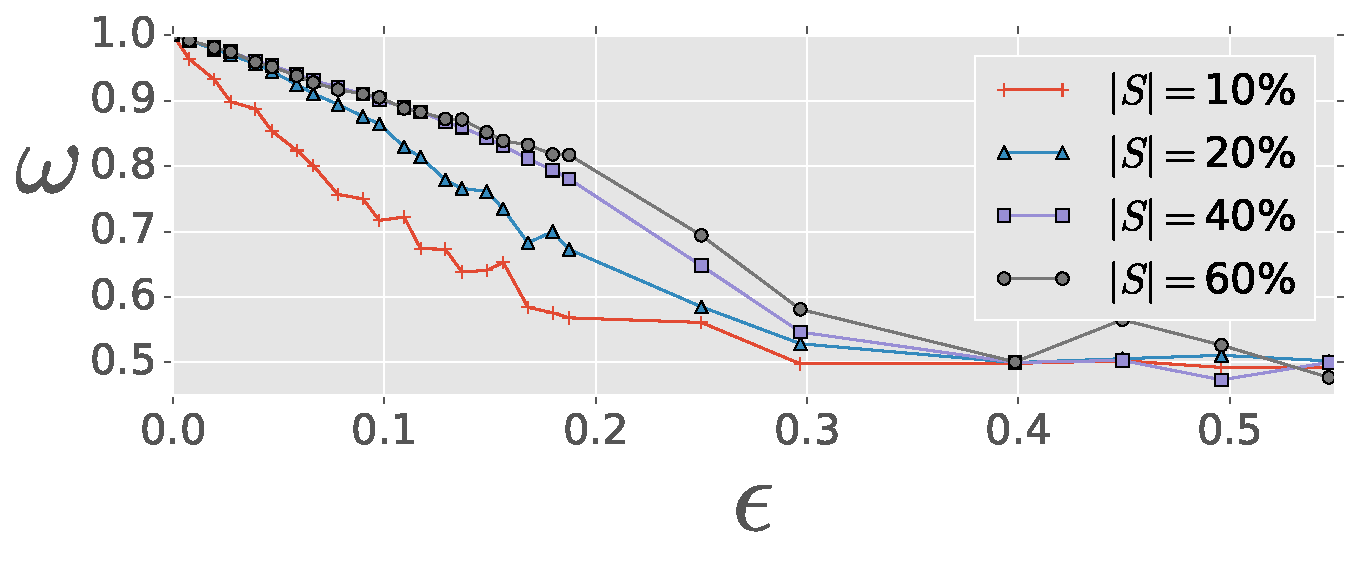
\includegraphics[scale=0.6]{figures/omega_vs_eps_dim8_nexp50_std_nEss8.pdf}
  \caption{$\omega$ for $\epsilon$-close functions to $L$.}
\label{omega_vs_eps}
\end{center}
\end{figure}

When $\epsilon = 0$ i.e. when $f_\epsilon$ is AP, we get $\omega = 1$ as expected from
Proposition \ref{PROPOS:AP_is_L}. We observe an almost linear decrease in $\omega$ as
$\epsilon$ grows to $0.3$ then leading to a plateau where $\omega =
\frac{1}{2}$, indicating that the analogical labels $\albl{\mathbf{x}}$ are
more or less random. Moreover, $\omega$ appears to decrease faster for small
training set $S$. This is due to the fact that the analogical labels
$\albl{\mathbf{x}}$ are the result of a majority-vote procedure among the
candidate solutions that one can build from $S$, and the number of candidates
becomes smaller as $\mid S\mid$ decreases, thus altering the quality of the
prediction.

We only have an empirical study here. Ultimately, it would be very interesting
to prove a result like
$$P(\omegasf \geq \eta) > 1 - \delta,$$
where $\eta \in [0, 1]$ and $\delta \in [0, \frac{1}{2}]$ is a function
$\epsilon$ and $\mid S \mid$. Such a result would be strongly linked to the PAC
learning theory \cite{Val72}, and is the object of current research.



We have studied so far the variation of $\omegasf$ when $f$ deviates from
the set of affine functions. We now focus on another point: the variation of
$\omegasf$ when $f$ deviates from being AP in a different way.
Let us note the following point: even if a function $f$ is far from being
AP, the quality $\omegasf$ of the extension $\esf$ may still be very
high. To illustrate this, let us define the value $\beta$ which is an indicator
of how far is $f$ from being completely AP.  For each $\mathbf{x} \in
\esfs$, we define $\beta_\mathbf{x}$ as the proportion of
candidates $\sol(f(\mathbf{a}), f(\mathbf{b}), f(\mathbf{c}))$ (with
$(\mathbf{a}, \mathbf{b}, \mathbf{c}) \in \rsfx$) that led to the the correct
label, i.e. the proportion of candidate solutions that are equal to
$f(\mathbf{x})$. $\beta$ is defined as the average of all the
$\beta_\mathbf{x}$.  Obviously, a function $f$ is AP iff $\beta = 1$ for all
$S$, i.e. if $\beta_\mathbf{x} = 1$ for all $\mathbf{x} \in \esfs$
and for all $S$.

Table \ref{table_monks} reports the values of $\omega$ and $\beta$ over three
datasets from the UCI repository, namely the three Monk's problems\footnote{As
these datasets are nominally-valued, they are binarized.} \cite{UCIrepo}.
Results are averaged over 100 experiments, where the training set $S$ is each
time randomly sampled with a size of $30$\% of the universe of possible
instances.

\begin{table}
\centering
\begin{tabular}{ c  c  c }
\toprule
  & $\omega$  & $\beta_S$ \\
\midrule
Monk 1 & .96 & .73 \\
Monk 2 & .96 & .69 \\
Monk 3 & .98 & .87 \\
\bottomrule
\end{tabular}
\caption{$\omega$ and $\beta$ over the Monk's problems.}
\label{table_monks}
\end{table}

We observe that for each dataset, $\beta$ is significantly lower than $1$.
This suggests that the Boolean functions underlying these datasets are highly
not AP, because on average, there is a high proportion (around $20$\%) of
candidates that predicted the wrong label. However, $\omega$ is no lower than
$96$\%, implying extensions of very high quality.  \textbf{This is where the
majority-vote comes into play}: in some cases, it may be able to compensate for
the predictors that were wrong.  This is what happens here in $96$\%, $96$\%
and $98$\% of the cases respectively. Here again, obtaining theoretical
guarantees about the majority vote procedure is currently investigated.

In the next subsection, we will extend our theoretical results about Boolean AP
functions to the a more general setting where instances are nominally valuated.

\subsection{Extension to nominal attributes}
\label{SEC:extension_to_nominal_attributes}

When it comes to real life applications, it is quite rare to get a purely
Boolean dataset.  It is generally the case that the dataset  is  a mix between
Boolean attributes and nominal attributes taking their values in finite sets.
For instance, an attribute \textit{color} typically takes its values in, let us
say, $\Set{red, green,blue}$. Unfortunately, on this set of values for attribute
\textit{color}, there is no structure, no order and no known operator.
Nevertheless, there is still a way to deal with such attributes within the
analogical framework, and to characterize AP functions in such settings. This
is what we investigate in this subsection.
 

We have already seen in Chapter \ref{CHAP:formal_analogical_proportions} that we
can define an analogical proportion on a set $X$ by restricting the accepted
analogical patterns to $a:b::a:b$ and $a:a::b:b$.  Formally, an analogy $A$
over $X$ is a subset of $X^4$ defined as:
$$A \eqdef \Set{ (a,a,b,b)  | a, b \in X} \cup \Set{ (a,b,a,b) | a, b \in X}$$

Back to the \textit{color} attribute, it means that we consider
$red:blue::red:blue$ as a valid analogical proportion but $red:blue::red:green$
is not valid. We can easily extend component-wise this analogy to a Cartesian
product $X^m=\prod_{i=1}^m X_i$ which is now equipped with an analogical
relation. In classification, this allows to deal with any kind of nominal
attributes.  In this setting, a binary classification function $f$ is a
function from $X^m=\prod_{i=1}^m X_i$ to $\mathbb{B}$. The question we want to
address here is the same as that of Section
\ref{SEC:a_complete_characterization_of_AP_functions}: we want to characterize all
the functions $f$ that lead to a perfectly sound analogical extension.
Unfortunately, we cannot turn to the previous framework because the Cartesian
product $X^m$ is made of distinct sets and is not anymore a power of
$\mathbb{B}$. So we will not be able to entirely identify these functions,
simply because we do not even know how to \textit{write} them. When dealing
with Boolean functions we used an algebraic point of view that allowed us
to write the functions in their Algebraic Normal Form, and we identified the AP
functions as those which have a particular ANF. But here this will not be
possible because there are no algebraic structure on the Cartesian product that
is the domain of our functions.

Nonetheless, we will still find close links between the AP Boolean functions
and the AP functions of our current setting, and these links are based on the
\textit{binarization} of the nominal attribute. Indeed, any nominal attribute
with $k$ values can be binarized into $k$ Boolean attributes. We can also choose
$k- 1$ attributes, or some other fancy binarization procedure, but we will
stick to the simplest one:
binarizing the \textit{color} attribute leads to three binary attributes
$(is\_red, is\_green, is\_blue)$ so that $red$ value is coded as $(1, 0, 0)$,
$green$ is coded as $(0, 1 , 0)$ and $blue$ is coded as $(0, 0, 1)$. Obviously,
the $k$ Boolean attributes are not independent: for example $(1, 1, 1)$  is not
a valid value.  More formally, let us denote $\bin$ this injective embedding
going from $X_i=\{v_1, \cdots, v_k\}$ to $\mathbb{B}^k$:
$$\bin(v_i) \eqdef (0, \cdots, 0, 1, 0, \cdots 0),$$
where $1$ is at position $i$.  So if we have a set of nominal attributes $x_1,
\cdots, x_m$ where $x_i$ takes its values in a finite set $X_i$, the Cartesian
product  $\prod_{i=1}^m X_i$ can be mapped into the set $\prod_{i=1}^m
\mathbb{B}^{\mid X_i \mid}$ by applying the injective embedding $\bin$ in a
component-wise fashion:
$$\bin(\prod_{i=1}^m X_i) \eqdef \prod_{i=1}^m  \bin(X_i).$$

From the very definition of this embedding, we have the following immediate and
obvious property:
\begin{property}
  \label{PROPER:analogy_nominal_iff_analogy_bin}
  For any $\mathbf{a}, \mathbf{b}, \mathbf{c}, \mathbf{d} \in X^m =
  \prod_{i=1}^m X_i$,
$$\mathbf{a}: \mathbf{b}:: \mathbf{c}: \mathbf{d} \iff
 \bin(\mathbf{a}): \bin(\mathbf{b}):: \bin(\mathbf{c}):
  \bin(\mathbf{d}).$$
 \end{property}
 \noindent
 Note that the proportion $\mathbf{a}: \mathbf{b}:: \mathbf{c}: \mathbf{d}$
 holds in $X^m$ while the proportion $\bin(\mathbf{a}): \bin(\mathbf{b})::
 \bin(\mathbf{c}): \bin(\mathbf{d})$ is a usual Boolean proportion that holds
 in $\prod_{i=1}^m\mathbb{B}^{\mid X_i \mid}$.  Now, every function $f$ from
 $\prod_{i=1}^n X_i$ to $\mathbb{B}$ can be associated to a \textbf{partial}
 Boolean function $f^b$ from $\prod_{i=1}^m \mathbb{B}^{|X_i|}$ to $\mathbb{B}$
 where $f^b$ is defined as follows:
$$
f^b(\bin(\mathbf{x})) \eqdef f(\mathbf{x})
$$

As the initial nominal universe  $\prod_{i=1}^m X_i$  has been compiled into a
Boolean universe, it is tempting to consider the framework that has been
developed in Section \ref{SEC:a_complete_characterization_of_AP_functions}.
Unfortunately, the whole set $\prod_{i=1}^m \mathbb{B}^{\mid X_i\mid}$ is not
the exact image of $\prod_{i=1}^m X_i$: it is bigger, and some elements in
$\prod_{i=1}^m  \mathbb{B}^{\mid X_i\mid}$ are not the image of an element of
$\prod_{i=1}^m X_i$ using $\bin$.  Ultimately, the domain of $f^b$ is just
$\bin(\prod_{i=1}^m X_i)$, which is included in $\prod_{i=1}^m
\mathbb{B}^{|X_i|}$. This is why $f^b$ is considered to be a partial function.

Nevertheless, the AP property is still relevant for functions that are only
partially defined: a partially defined function that always lead to a perfectly
sound analogical extension for any training set $S$ will also be said to be
Analogy Preserving, and will be called PAP for Partial AP. Just like in Section
\ref{SEC:a_complete_characterization_of_AP_functions}, a natural way to
characterize PAP functions is given in Definition \ref{DEF:PAP_functions}:

\begin{definition}[Partial analogy preserving functions]
  \label{DEF:PAP_functions}
  A partial function $f^b$ is {\bf Analogy Preserving} (PAP)
  if for all $\mathbf{a}, \mathbf{b}, \mathbf{c}, \mathbf{d} \in
  \text{dom}(f^b)$,:
  $$
  \begin{cases}
    \mathbf{a} :  \mathbf{b} ::  \mathbf{c} :  \mathbf{d} \text{ and }\\
    solvable(f^b(\mathbf{a}),f^b(\mathbf{b}),f^b(\mathbf{c}))
  \end{cases}
  \implies \text{sol}(f^b(\mathbf{a}),f^b(\mathbf{b}),f^b(\mathbf{c})) =
  f^b(\mathbf{d}).
  $$
\end{definition}

Proposition \ref{PROPOS:PAP_eq_AP} will provide us with the link between $f$
and $f^b$, when one of them is AP:

\begin{proposition}
  \label{PROPOS:PAP_eq_AP}
Let $f$ be a function from $\prod_{i=1}^n X_i$ to $\mathbb{B}$. Then $f$ is AP
if and only if $f^b$ is PAP.
\end{proposition}
\begin{proof}
  Let us assume that $f$ is AP and let be 4 elements belonging to the domain of
  $f^b$: $\bin(\mathbf{a}),\bin(\mathbf{b}), \bin(\mathbf{c}), \bin(\mathbf{d})
  \in \bin(\prod_{i=1}^m X_i)$ such that:
  $$\begin{cases}
    \bin(\mathbf{a}):\bin(\mathbf{b})::\bin(\mathbf{c}):\bin(\mathbf{d}) \mbox{
      and}\\
    \solvable(f^b(\bin(\mathbf{a})),f^b(\bin(\mathbf{b})),f^b(\bin(\mathbf{c}))).
  \end{cases}
  $$
Thanks to Property \ref{PROPER:analogy_nominal_iff_analogy_bin}, we have seen
  that in this case we also have
  $\mathbf{a}:\mathbf{b}::\mathbf{c}:\mathbf{d}$.  Since by definition
  $f(\mathbf{x}) = f^b(\bin(\mathbf{x}))$,  the second condition simply is
  $\solvable(f(\mathbf{a}),f(\mathbf{b}),f(\mathbf{c}))$. As $f$ is AP,
  $\sol(f(\mathbf{a}),f(\mathbf{b}),f(\mathbf{c}))= f(\mathbf{d})$, and
  $f(\mathbf{d}) = f^b(\bin(\mathbf{d}))$. So in the end, we have that
  $\sol((f^b(\mathbf{a}),f^b(\mathbf{b}),f^b(\mathbf{c})) =
  f^b(\bin(\mathbf{d})$, which proves that $f^b$ is PAP.

  Let us now focus on the reverse implication. Consider a PAP function
  $f^b$ and 4 elements $\mathbf{a}, \mathbf{b}, \mathbf{c}, \mathbf{d} \in
  \prod_{i=1}^m X_i$ such that:
  $$
  \begin{cases}
  \mathbf{a}:\mathbf{b}::\mathbf{c}:\mathbf{d} \mbox{ and}\\
  \solvable(f(\mathbf{a}),f(\mathbf{b}),f(\mathbf{c}))
  \end{cases}
  $$
  Thanks again to Property \ref{PROPER:analogy_nominal_iff_analogy_bin},
  $\bin(\mathbf{a}):\bin(\mathbf{b})::\bin(\mathbf{c}):\bin(\mathbf{d})$ holds. 
  The second condition is just
  $\solvable(f^b(\bin(\mathbf{a})),f^b(\bin(\mathbf{b})),f^b(\bin(\mathbf{c})))$
  because by definition, $f(\mathbf{x}) = f^b(\bin(\mathbf{x}))$. Be cause
  $f^b$ is PAP, we have that
  $\sol(f^b(\bin(\mathbf{a})),f^b(\bin(\mathbf{b})),f^b(\bin(\mathbf{c}))) =
  f^b(\bin(\mathbf{d}))$. As $f^b(\bin(\mathbf{d}))=f(\mathbf{d})$ by
  definition, we have that $f$ is AP.
\end{proof}

In the end, the notions of AP function is smoothly transferable to the notion
of PAP function. This result is only purely theoretical, and sadly there are
not much we can extract from it for practical use. Proposition
\ref{PROPOS:PAP_eq_AP} tells us that when dealing with nominal attributes, if
the function underlying the ground truth labels is affine once the dataset has
been binarized, then we can safely extend our training set. Unfortunately, as
there are no common operators on the set  $\prod_{i=1}^n X_i$, we are not able
to give a more accurate characterization of AP functions in such settings.

In the next subsection, however, we will see that in a real setting the AP
functions are also precisely the affine (real) functions.

\subsection{Extension to real-valued functions}
\label{SEC:extension_to_real_valued_functions}

Section \ref{SEC:a_complete_characterization_of_AP_functions} was devoted to the
identification of Boolean functions that where fully compatible with the
analogical inference principle, and we saw that
these functions are the Boolean affine functions. One may wonder what would
these functions be in a real setting, i.e. using functions  from $\mathbb{R}^m$
to $\mathbb{R}$ with the arithmetic proportion?

Well, we already know that the Boolean proportion and the arithmetic proportion
are really close. Once again, we will witness this close bond: in a real
setting, the class of AP functions is also the class of real linear functions.
Luckily, the proof is a lot easier to derive.  Let us first (re)define the
arithmetic proportion:
\begin{property}
  \label{PROPER:sol_arithm_prop}
  Four elements $\mathbf{a}, \mathbf{b}, \mathbf{c}, \mathbf{d} \in
  \mathbb{R}^m$ are in arithmetic proportion if $\mathbf{d} = \mathbf{c} -
  \mathbf{a} + \mathbf{b}$.

  Also, for any $a, b, c \in \mathbb{R}$, the equation $a : b :: c:y$ is always
  solvable and the solution is $\emph{sol}(a, b, c) = c - a + b$.
\end{property}

Please note that here, the $+$ is the regular addition operator (not the modulo
2 addition as in the previous sections). We will also use a simple property of
affine functions:

\begin{property}
  \label{PROPRE:f_affine_real}
  A real function $f$ from $\mathbb{R}^m$ to $\mathbb{R}$ is affine if f is of
  the form: $$f(\mathbf{x}) = \boldsymbol{\alpha} \cdot \mathbf{x} +
  \alpha_0.$$ where $\boldsymbol{\alpha} \in \mathbb{R}^m$ and $\alpha_0  =
  f(\mathbf{0}) \in \mathbb{R}$.
  Also, $f$ is affine iff $\forall \mathbf{a}, \mathbf{b}, \mathbf{c} \in
  \mathbb{R}^m$:

  $$f(\mathbf{c} - \mathbf{a} + \mathbf{b}) = f(\mathbf{c}) - f(\mathbf{a}) +
  f(\mathbf{b}).$$
\end{property}
\begin{proof}
  Let $f$ be an affine function.
  $\forall \mathbf{a}, \mathbf{b}, \mathbf{c} \in \mathbb{R}^m$,
  \begin{align*}
    f(\mathbf{c} - \mathbf{a} + \mathbf{b}) &= \boldsymbol{\alpha} \cdot (\mathbf{c}
    - \mathbf{a} + \mathbf{b}) + \alpha_0\\
    &= \boldsymbol{\alpha} \cdot \mathbf{c} - \boldsymbol{\alpha} \cdot
    \mathbf{a} + \boldsymbol{\alpha} \cdot \mathbf{b} + \alpha_0\\
    &= f(\mathbf{c}) - f(\mathbf{a}) + f(\mathbf{b}).
  \end{align*}

  Now, let $f$ be a function such that $f(\mathbf{c} - \mathbf{a} +
  \mathbf{b}) = f(\mathbf{c}) - f(\mathbf{a}) + f(\mathbf{b})$, and consider
  the function $g$ defined by $g(\mathbf{x}) = f(\mathbf{x}) - f(\mathbf{0}).$

  \begin{align*}
    g(\mathbf{x} + \mathbf{y}) &= f(\mathbf{x} + \mathbf{y}) - f(\mathbf{0})\\
    &= f(\mathbf{x} - \mathbf{0} + \mathbf{y}) - f(\mathbf{0})\\
    &= f(\mathbf{x}) + f(\mathbf{y}) - 2f(\mathbf{0})\\
    &= g(\mathbf{x}) + g(\mathbf{y})
  \end{align*}

  So $g(\mathbf{x} + \mathbf{y}) = g(\mathbf{x)} + g(\mathbf{y})$ and by
  definition, $g$ is linear and $g$ can be written as:
  $$g(\mathbf{x}) = \boldsymbol{\alpha} \cdot \mathbf{x}.$$

  So $f(\mathbf{x}) = \boldsymbol{\alpha} \cdot \mathbf{x} + f(\mathbf{0}),$
  which makes $f$ affine.
\end{proof}

We now prove that the real AP functions are the real affine functions, just
like the Boolean AP functions are the Boolean affine functions.

\begin{proposition}
  \label{PROPOS:arithm_AP_func_affine_func}
  With the arithmetic proportion, the set of real AP functions from
  $\mathbb{R}^m$ to $\mathbb{R}$ is the set of affine functions.
\end{proposition}
\begin{proof}
  A real function $f$ is AP iff for all $\mathbf{a}, \mathbf{b}, \mathbf{c},
  \mathbf{d} \in \mathbb{R}^m$,

  $$\mathbf{a}: \mathbf{b}:: \mathbf{c}: \mathbf{d} \implies
  \sol(f(\mathbf{a}), f(\mathbf{b}), f(\mathbf{c})) = f(\mathbf{d}).$$

  Equivalently, thanks to property \ref{PROPER:sol_arithm_prop},  $f$ is AP
  iff: $$\mathbf{d} = \mathbf{c} - \mathbf{a} + \mathbf{b} \implies
  f(\mathbf{c}) - f(\mathbf{a}) +  f(\mathbf{b}) = f( \mathbf{c} - \mathbf{a} +
  \mathbf{b}).$$

  From Property \ref{PROPRE:f_affine_real}, this is true iff $f$ is affine.
\end{proof}

Proposition \ref{PROPOS:arithm_AP_func_affine_func} is illustrated in Figure
\ref{FIG:real_AP_func}.
\begin{figure}[!h]
\centering
  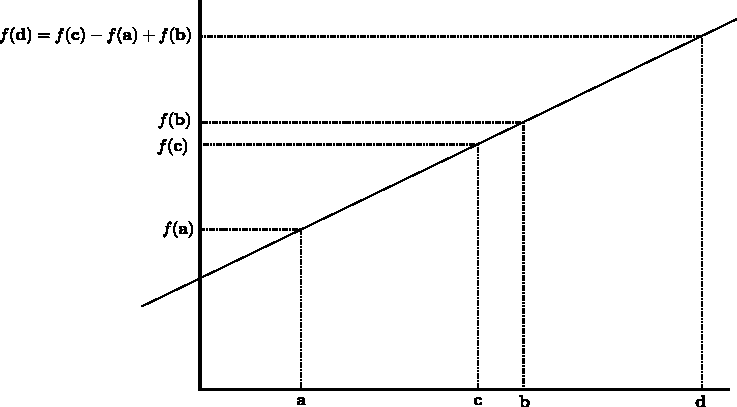
\includegraphics[width=3.5in]{figures/real_AP_fuction.pdf}
  \caption{When $f$ is affine, $\sol(f(\mathbf{a}), f(\mathbf{b}),
  f(\mathbf{c})) = f(\mathbf{d})$.}
\label{FIG:real_AP_func}
\end{figure}

In fact, Proposition \ref{PROPOS:AP_is_L} for Boolean functions can be
proved in a much simpler way than what was used in Section
\ref{SEC:a_complete_characterization_of_AP_functions}, using
the same outline as Proposition \ref{PROPOS:arithm_AP_func_affine_func}. The
first step is to see that a Boolean function is affine iff $f(\mathbf{a} +
\mathbf{b} + \mathbf{c}) = f(\mathbf{a}) + f(\mathbf{b}) + f(\mathbf{c})$,
where $+$ is now the module 2 addition. Also, noting that $\mathbf{a} :
\mathbf{b} :: \mathbf{c} : \mathbf{d} \implies \mathbf{d} = \mathbf{a} +
\mathbf{b} + \mathbf{c}$ and that for any $a, b, c \in \mathbb{B}$ we have
$\sol(a, b, c) = a + b + c$, the proof can be derived easily. We chose to give
the longest one in Section \ref{SEC:a_complete_characterization_of_AP_functions} because this is the one that was
originally derived.\todo{And it was in IJCAI paper?}

\section*{Conclusion}

The main contribution of this chapter was to provide a complete
characterization of Boolean functions that are fully compatible with the
analogical inference principle that we have used so far in all the previous
chapters of this document. Using an appropriate representation for Boolean
functions (namely their algebraic normal form), we have been able to prove that
the class of AP functions is the class of affine functions, i.e. functions
whose degree is less than $1$.

We chose to tackle the problem of finding the class of AP functions from the
angle of training set extension. It became clear that the class of AP functions
can be seen as the class of functions that allow  a perfectly sound extension,
or equivalently as the class that allow the analogical inference principle to
be sound.

We also provided a more explicit version of the analogical inference principle
which is in fact less restrictive than the one we have claimed so far. The
distinction between the strict version and the relaxed version is that the
class equation $f(\mathbf{a}) : f(\mathbf{b}) ::f(\mathbf{c}) :y$ is not always
solvable, and the relaxed version takes this fact into account. The class of AP
functions is fully compatible with the relaxed version, but we have also
identified the functions that are compatible with the strict version, which
turned out to be the class of projections (or dictators) functions.

In real-world application though, purely affine functions are extremely rare.
This means that using the analogical inference principle will necessarily
produce errors in the label predictions. We have empirically investigated the
quality of the analogical extension (which measures in some sense how
\textit{adequate} was the use of the analogical inference principle) when a
function deviates from the class of purely affine functions. We have observed
that the quality of the extension linearly decreases, but a strong statistical
result still needs to be derived. We also noted that in some particular cases,
a function that is strongly not AP can still lead to a high extension quality.
Indeed, as the analogical labels are the result of a majority-vote procedure,
it may happen that the most common candidate label actually corresponds to the
ground truth label $f(\mathbf{x})$. In this case, the majority-vote procedure
is able to compensate of the candidates that were wrong in their predictions,
because it will choose the most common predictor which happens to be the
correct label.  Ultimately, even if only $50\% + \epsilon$ ($\epsilon > 0$) of
the candidates are correct, it is still enough to have a perfectly sound
extension. The class of AP functions ensure that exactly $100\%$ of the
candidates are correct, but it is clear that such a requirement is too strong
to be really useful in practice. The derivation of a theoretical result
involving the role  of the majority-vote procedure is still a topic of current
research.

Our main goal was to identify the class of AP functions in a Boolean setting.
We have extended our results to two other domains. It is often the case that
the classification problem does not involve purely Boolean attribute, but
rather a more general domain where instances are multi-valuated. Sadly in these
domains, there are no know structure or operators, so it was not possible to
give a clear identification of AP functions such as that of Boolean AP
functions. We were however able to provide a clear link between these AP
functions and the Boolean AP functions by embedding the multi-valuated space
into a partially defined Boolean space. We also provided a clear identification
of AP functions in a real setting, i.e. for functions from $\mathbb{R}^m$ to
$\mathbb{R}$. It turns out that the class of real AP functions is the class of
real affine functions, just like the class of Boolean AP functions is the class
of Boolean affine functions. The result for real functions was much easier to
prove and in the end quite trivial, and seems to strongly limit use of the
analogical inference principle in a real setting.


\chapter*{Conclusion}
\addcontentsline{toc}{chapter}{Conclusion} % To add to TOC

\initial{I}t is now time to conclude this document, whose purpose was twofold:
exhibit clear theoretical properties of analogical classifiers, and apply
analogical inference to the field of recommender systems. Let us first recap
our main results and contributions (we will not necessarily follow the order of
the chapters here).

\paragraph{Contributions\\}

The first chapter was dedicated to give the necessary background on existing
models of analogical reasoning,  with a strong emphasis on models that allowed
to build computer programs. In the second chapter, we thoroughly described
various definitions of analogical proportions in different settings, with a
particular focus on the arithmetic and Boolean proportions. We have tried to
provide the reader with different geometrical insights on these proportions,
which were hopefully useful to gain a better intuition.
Finally, we considered a toy classification problem in a Boolean setting that
allowed us to introduce the analogical equation solving process and most
importantly, our analogical inference principle. This principle states that if
we have $a:b::c:d$, then we should also have $f(a) : f(b) :: f(c):f(d)$, where
$f(x)$ is the label of $x$, or any characteristic of interest.  When $f(d)$ is
unknown, it can be \textbf{inferred} from the values of $f(a)$, $f(b)$ and
$f(c)$, allowing us to apply this form of analogical reasoning to
classification tasks, or more general problems such as that of rating
prediction for recommendation tasks.\\

Analogical recommendation was addressed in Chapters
\ref{CHAP:background_reco_systems} and \ref{CHAP:analogical_recommendation}.
Chapter \ref{CHAP:background_reco_systems} was a background chapter, where we
clearly defined the problem we planned to address, and described two popular
collaborative filtering families (neighborhood methods and
matrix-factorization techniques) that will be compared to our custom algorithms
in the experiments.

We then developed in Chapter \ref{CHAP:analogical_recommendation} an algorithm
for rating prediction \cite{HugPraRicISMIS15}, on the basis that if four users
are in proportion (i.e. their respective ratings are in arithmetic proportion),
then it should also be the case for any item that one of the four users has not
rated. This approach is directly inspired from past works on analogical
classification. The experiments showed that this algorithm offers reasonable
performance compared to neighborhood techniques, but its cubic complexity makes
it simply impossible to use in real-world scenarios, due to enormous
computation time.

This led us to consider another kind of analogical recommendation, that does
not rely on the search of $3$-tuples of users. This ``clone''-based view
\cite{HugPraRicSerFuzzIEEE16} is motivated by the fact that some users may
have different interpretations of the rating scale that is used. Our results
show that the concept of ``clone'' is extremely relevant, but it must be noted
that this kind of bias in the user ratings had already been addressed in
previous works.

Finally, we provided an algorithm for the mining of analogical proportions in
incomplete databases \cite{HugPraRicSerLFA16}, strongly inspired from the
mining of association rules. We used this algorithm to extract analogical
proportions between items in a rating database, which actually corresponds to
the database that we had been using for our recommendation experiments. Our
results showed that the analogies we found were in fact rather
uninteresting, in that they related four items that were either equally
appreciated, or equally disliked. There was no discrepancy in the ratings. In
a way, this fact can retrospectively explain the modest results of our first
analogical recommendation algorithm, and its performances that were close to
those of neighborhood methods.\\

In Chapter \ref{CHAP:functional_definition}, we described our contributions to
the field of analogical classification \cite{HugPraRicSerECAI16}. Our first key
contribution was to provide a unifying functional definition of analogical
classifiers, which were yet only known from their algorithmic descriptions.
From this definition, we were able to derive various theoretical properties. In
particular, we showed that the VC-dimension of analogical classifiers is
infinite, and that their error rate is closely related to that of the $k$-NN
algorithms, as can be seen on the analytical formula that we derived. In fact,
our functional definition establishes clear links between analogical
classification and nearest-neighbors classification. We have showed indeed that
analogical classification can be viewed as a two-steps procedure: first the
training set is extended by analogy, where new examples are generated and
assigned a potentially noisy label called the analogical label. Then, using
this extended training set, all the remaining elements can be labeled using the
classical $k$-NN procedure. This new point of view is quite interesting,
because it clearly binds together the two processes triggered by analogical
proportions (inference and creativity) as the two sides of the same coin.

In Chapter \ref{CHAP:analogy_preserving_functions}, we investigated a question
that naturally followed from the results of Chapter
\ref{CHAP:functional_definition}: how can we ensure that the analogical
extension is completely error-free? In other words, is there a criterion that
tells us that the new examples that are generated are associated to the correct
label? We have been able to answer this question in a Boolean setting: the
analogical extension is perfectly sound if and (only if) the Boolean function
$f$ underlying the label is an affine function. This strong result
\cite{CouHugPraRicIJCAI17} is reminiscent of that of Davies and Russel (see
Section \ref{SEC:Davies_and_Russel}), who provided a side condition that
allowed to safely use an analogical inference principle. Their analogical
inference principle was actually quite different from ours (although we could claim
that ours is a particular case of theirs), but the two approaches can be
considered similar from a general point of view. We extended our results to the
real setting and in the case where attributes are nominally-valued. These
results open the door to various speculative research topics, that we will now
explore.

\paragraph{Future work\\}

In Section \ref{SEC:approximate_ap_functions}, we presented the concept of
approximate AP functions. Indeed in practice, there is no way
to know for sure if the function $f$ that we want to learn is completely
affine. So a clear topic of interest is to obtain statistical guarantees about
the quality of the analogical extension, depending on how far the function $f$
is from the set of affine functions. As previously mentioned, a result of the
following form would be extremely interesting:
$$P(\omegasf \geq \eta) > 1 - \delta,$$
where $\eta \in [0, 1]$ and $\delta \in [0, \frac{1}{2}]$ are functions
depending on $\epsilon$ and $\mid S \mid$. The value $\epsilon$ tells us that
$f$ is $\epsilon$-close from the set of affine functions.  We are currently
investigating a somewhat simpler question:
$$P(\omegasf < 1) < \delta,$$
where $\delta$ is still a function of $\epsilon$. In other words, we want to
have an upper bound of the probability of the event ``\textit{$\esfs$ is
unsound}''.\\

We have also seen during our experimentations that even though some functions are
highly not AP, the quality of the analogical extension may still be very high.
This is because of the majority-vote procedure that is applied when we compute
the analogical label of the elements. This aspect has been left out of the
discussion so far, but it is clear that it is a decisive step of our inference
process, and it has to be thoroughly studied to fully understand the analogical
classification process. We may for example suppose that some $3$-tuples should
be given a higher weight in the aggregation, on the basis of some particular
static criterion that still needs to be identified.\\

Another track of research can be motivated by looking at Figure
\ref{FIG:piecewise_affine}.
\begin{figure}[!h]
\centering
  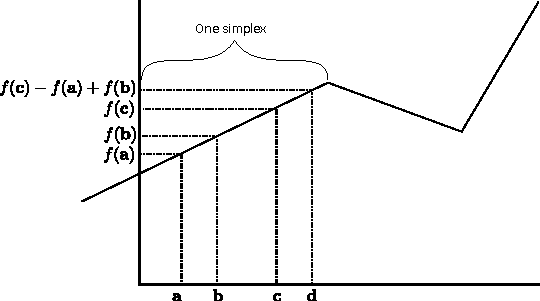
\includegraphics[width=3in]{figures/piecewise_affine.pdf}
  \caption{A real function $f$ that is piecewise affine.}
\label{FIG:piecewise_affine}
\end{figure}
The function $f$ is not affine, but is instead \textbf{piecewise affine}. We
know from our results that for any elements $\mathbf{a}, \mathbf{b},
\mathbf{c}, \mathbf{d} \in X^m$ that are on the same simplex (a simplex is here
defined as a subset of $X^m$ where $f$ is affine), then we can correctly
predict the value of $f(\mathbf{d})$ from those of $f(\mathbf{a}),
f(\mathbf{b}), f(\mathbf{c})$. Well in $\mathbb{R}^m$ this result is not really
useful, but we can actually show that every Boolean function is piecewise
affine! So theoretically, if we can identify all the simplices, this means that
we should be able to produce a sound extension in any case, for any function
$f$, and for any training set. At this point, only preliminary experiments
have been carried out, and a more thorough investigation deserves to be
addressed.\\

Finally, we will close this discussion by mentioning the elephant in the room
that we have so far ignored: transfer learning. Transfer learning is a current
trend in the machine learning community, whose purpose is to use the knowledge
of a source problem $S$, to apply it to a less known target problem $T$.
Undoubtedly, transferring knowledge is the essence of analogy, and techniques
in transfer learning usually involve statistical tools (see e.g.
\cite{PanYanTKDE10} for a survey). The use of analogical proportions for such
purposes is still entirely to be explored.


\backmatter
\bibliographystyle{alpha} % or named ?
\refstepcounter{chapter}
\bibliography{biblio}

\end{document}
